\documentclass[10pt,notes,compress,aspectratio=169]{beamer}
\usepackage[brazil]{babel}  
\usepackage[utf8]{inputenc}
\usepackage[T1]{fontenc}

\usefonttheme[onlymath]{serif}
\usepackage{beamerthemesplit}
\usetheme{Antibes}

\beamersetuncovermixins{\opaqueness<1->{25}}{\opaqueness<2->{15}}
\setbeamertemplate{itemize items}[triangle]
\setbeamertemplate{enumerate item}{\insertenumlabel)}
\setbeamertemplate{enumerate subitem}{\insertenumlabel-\insertsubenumlabel)}
\setbeamertemplate{caption}[numbered]
\setbeamertemplate{mini frames}{}
\setbeamertemplate{navigation symbols}{}
\setbeamerfont{block title}{size=\scriptsize}
\setbeamerfont{frametitle}{size=\small}
\beamertemplatenavigationsymbolsempty

%%%%%%%%%%%%%%%%%%%%%
% defining frametitle
\setbeamertemplate{frametitle}{%
    \nointerlineskip%
    \begin{beamercolorbox}[wd=\paperwidth,ht=2.5ex,dp=1.0ex]{frametitle}
        \hspace*{2.5ex}\insertframetitle%
    \end{beamercolorbox}%
}
%%%%%%%%%%%%%%%%%%%%%
\usepackage{color}
\definecolor{BlueGreen}{cmyk}{0.8,0,0.5,0.3}
\newcommand{\hrefcolor}[2]{\textcolor{BlueGreen}{\href{#1}{#2}}}

% Rotating Objects and Captions
\usepackage{hvfloat}

\usepackage{natbib}
\usepackage[brazilian]{cleveref}
\crefname{lstlisting}{lista}{listas}
\Crefname{lstlisting}{Lista}{Listas}

% equation stuff
\usepackage{nicefrac}
\usepackage{cancel}

% multi-do
\usepackage{multido}

% write algorithm
\usepackage{algorithm}
\usepackage{algpseudocode}

% table diagonal box
\usepackage{diagbox}
\usepackage{makecell}

% tables
\usepackage{booktabs}

% BEGIN - listings - code in LaTeX
\usepackage{listings}
\renewcommand\lstlistingname{Lista}
\lstset{
  language=octave,
  breaklines=true,
  postbreak=\mbox{$\hookrightarrow$\space},
  basicstyle=\linespread{1}\small\ttfamily,
  %numbers=left,
  numbers=none,
  %frame=lines,
  xleftmargin=0.5cm,
  frame=none,
  framexleftmargin=0.5em,
  framexrightmargin=0.5em,
  %backgroundcolor=\color{light-gray},
  showstringspaces=false,
  upquote=true,
  commentstyle=\color{gray},
  %morecomment=[f][\color{gray}][28]{\#},
  morecomment=[l]{\#\#},
  literate=%
           {á}{{\'a}}1
           {í}{{\'i}}1
           {é}{{\'e}}1
           {ú}{{\'u}}1
           {ó}{{\'o}}1
           {à}{{\`a}}1
           {ã}{{\~a}}1
           {õ}{{\~o}}1
           {â}{{\^a}}1
           {ê}{{\^e}}1
           {ô}{{\^o}}1
           {ç}{{\c{c}}}1
           {Á}{{\'A}}1
           {Í}{{\'I}}1
           {É}{{\'E}}1
           {Ú}{{\'U}}1
           {Ó}{{\'O}}1
           {À}{{\`A}}1
           {Ã}{{\~A}}1
           {Õ}{{\~O}}1
           {Â}{{\^A}}1
           {Ê}{{\^E}}1
           {Ô}{{\^O}}1
           {Ç}{{\c{C}}}1
}
% END - listings

% arydshln - Draw dash-lines in array/tabular
\usepackage{arydshln}

% adjust general LaTeX material in several way
\usepackage{adjustbox}

%\usepackage{multirow,graphicx,array}
\newcommand*\rot{\rotatebox{90}}

% flexible mechanism for giving coloured panels behind specified columns in a table
\usepackage{colortbl}

\usepackage{multirow}


%\usepackage{amsthm}
%\newtheorem{theorem}{Theorem}
%\newtheorem{corollary}{Corollary}
%\newtheorem{lemma}{Lemma}
\newtheorem{proposition}{Proposition}
\newtheorem{axiom}{Axiom}
%\newtheorem{example}{Example}
%\newtheorem{definition}{Definition}
\newtheorem{remark}{Remark}

\usepackage{etoolbox}
\patchcmd{\theorem}{Theorem}{Teorema}{}{}
\patchcmd{\corollary}{Corollary}{Corolário}{}{}
\patchcmd{\lemma}{Lemma}{Lema}{}{}
\patchcmd{\proposition}{Proposition}{Proposição}{}{}
\patchcmd{\axiom}{Axiom}{Axioma}{}{}
\patchcmd{\example}{Example}{Exemplo}{}{}
\patchcmd{\definition}{Definition}{Definição}{}{}
\patchcmd{\remark}{Remark}{Observação}{}{}

%\patchcmd{\theorem}{Theorem}{Teorema}{}{}
%\patchcmd{\corollary}{Corollary}{Corolário}{}{}
%\patchcmd{\lemma}{Lemma}{Lema}{}{}
%\patchcmd{\proposition}{Proposition}{Proposição}{}{}
%\patchcmd{\axiom}{Axiom}{Axioma}{}{}
%\patchcmd{\example}{Example}{Exemplo}{}{}
%\patchcmd{\definition}{Definition}{Definição}{}{}
%\patchcmd{\remark}{Remark}{Observação}{}{}

\newtheorem{exercise}{Exercício}

\newcommand*{\theorembreak}{\usebeamertemplate{theorem end}\framebreak\usebeamertemplate{theorem begin}}
\newcommand*{\proofbreak}{\hfill ...\usebeamertemplate{proof end}\framebreak\usebeamertemplate{proof begin}{\scriptsize\color{gray}continuação...}\\}
\newcommand*{\examplebreak}{\hfill ...\usebeamertemplate{theorem end}\framebreak\usebeamertemplate{theorem begin}{\scriptsize\color{gray}continuação...}\\}
\newcommand*{\exercisebreak}{\hfill ...\usebeamertemplate{theorem end}\framebreak\usebeamertemplate{theorem begin}{\scriptsize\color{gray}continuação...}\\}
\newcommand*{\lemmabreak}{\hfill ...\usebeamertemplate{theorem end}\framebreak\usebeamertemplate{theorem begin}{\scriptsize\color{gray}continuação...}\\}
\newcommand*{\blockbreak}{\hfill ...\usebeamertemplate{block end}\framebreak\usebeamertemplate{block begin}{\scriptsize\color{gray}continuação...}\\}
\newcommand*{\definitionbreak}{\hfill ...\usebeamertemplate{theorem end}\framebreak\usebeamertemplate{theorem begin}{\scriptsize\color{gray}continuação...}\\}

% math symbols

% symbol for independet
\newcommand\independent{\protect\mathpalette{\protect\independenT}{\perp}}
\def\independenT#1#2{\mathrel{\rlap{$#1#2$}\mkern2mu{#1#2}}}
% Real Numbers
\newcommand\RealNumber{{\rm I\!R}}
% Expected value, Variance and Covariance
\newcommand{\E}{\mathrm{E}}
\newcommand{\Var}{\mathrm{Var}}
\newcommand{\Cov}{\mathrm{Cov}}

%%%%%%%%%%%%%%%%%
% math cancel to (down arrow)
\makeatletter
% #1, #2 offset of label   #6 extra width to clear arrowhead
% #3, #4 vector direction  #7 superscript label style
% #5 vector width          #8 superscript label
\def\cantox@vector#1#2#3#4#5#6#7#8{%
  \dimen@.5\p@
  \setbox\z@\vbox{\boxmaxdepth.5\p@
   \hbox{\kern-1.2\p@\kern#1\dimen@$#7{#8}\m@th$}}%
  \ifx\canto@fil\hidewidth  \wd\z@\z@ \else \kern-#6\unitlength \fi
  \ooalign{%
    \canto@fil$\m@th \CancelColor
    \vcenter{\hbox{\dimen@#6\unitlength \kern\dimen@
      \multiply\dimen@#4\divide\dimen@#3 \vrule\@depth\dimen@\@width\z@
      \vector(#3,-#4){#5}%
    }}_{\raise-#2\dimen@\copy\z@\kern-\scriptspace}$%
    \canto@fil \cr
    \hfil \box\@tempboxa \kern\wd\z@ \hfil \cr}}
\def\bcancelto#1#2{\let\canto@vector\cantox@vector\cancelto{#1}{#2}}
\makeatother
%%%%%%%%%%%%%%%%%


%%%%%%%%%%%%%%%%%
% left-right arrow
\makeatletter
\newcommand\xleftrightarrow[2][]{%
  \ext@arrow 9999{\longleftrightarrowfill@}{#1}{#2}}
\newcommand\longleftrightarrowfill@{%
  \arrowfill@\leftarrow\relbar\rightarrow}
\makeatother
%%%%%%%%%%%%%%%%%


%%%%%%%%%%%%%%%%%
% commands to resume enumeration across frames 
\newcounter{sauvegardeenumi}
\newcommand{\asuivre}{\setcounter{sauvegardeenumi}{\theenumi}}
\newcommand{\suite}{\setcounter{enumi}{\thesauvegardeenumi}}
%%%%%%%%%%%%%%%%%

%%%%%%%%%%%%%%%%% underbrase - font size no change
\newcommand*{\KeepStyleUnderBrace}[1]{%
  \mathop{%
    \mathchoice
    {\underbrace{\displaystyle#1}}%
    {\underbrace{\textstyle#1}}%
    {\underbrace{\scriptstyle#1}}%
    {\underbrace{\scriptscriptstyle#1}}%
  }\limits
}
%%%%%%%%%%%%%%%%%

%%%%%%%%%%%%%%%%% math operators
\DeclareMathOperator*{\argmin}{\arg\!\min}
\DeclareMathOperator*{\argmax}{\arg\!\max}
\DeclareMathOperator{\sign}{sign}
\DeclareMathOperator{\Tr}{Tr}
%%%%%%%%%%%%%%%%%


%%%%%%%%%%%%%%%%%
\newenvironment{inlineitemize}{%
 \let\par\relax%
 \def\item{\usebeamertemplate{itemize item}\hspace{1mm}}
 \leavevmode%
}{}

\newenvironment{inlineenumerate}{%
 \let\par\relax%
 \setcounter{enumi}{1}%
 \def\item{\usebeamertemplate{enumerate  item} \stepcounter{enumi}}%
 \leavevmode%
}{%
 \setcounter{enumi}{0}%
}
%%%%%%%%%%%%%%%%%




\title[Teoria da Informação]{Teoria da Informação}
\author[Prof. Leonardo Araújo]{Prof. Leonardo Araújo}
\date{}


\begin{document}
\frame{\titlepage}

\frame{\centering 
\includegraphics[width=0.4\textwidth]{images/qrcode-ti.pdf} \\ \url{https://sites.google.com/site/leolca/teaching/information-theory}}
\frame{\centering 
\includegraphics[width=0.4\textwidth]{images/qrcode-slides.pdf} \\ \url{https://github.com/leolca/lectures/blob/master/ti/teoria-da-informacao.pdf}}



\frame[allowframebreaks]{\begin{footnotesize}\tableofcontents\end{footnotesize}}

% introdução
\section{Introdução}

\begin{frame}%[allowframebreaks]
  \frametitle{Processamento de Áudio e Vídeo}
 
  \begin{itemize}
  \item Compressão
  \item Com/Sem perdas
  \item mp3, jpeg, mpeg, flac, zip, gif, png, etc
  \item sinais de áudio, fala, imagens e vídeo
  \item qualidade, taxa de compressão, custo
  \end{itemize} 

\end{frame}
\note{
  \begin{itemize}
  \item O conceito de compressão surge naturalmente quando estamos lidando com comunicação.
  \item Compressão de dados é o processo de converter dados provenientes de uma fonte em
  outros dados com menor tamanho.
  \item Armazenamento e transmissão (no fundo, ambos são formas de comunicação). 
    \begin{itemize}
    \item linha telefônica analógica
    \item comunicação digital através desta linha telefônica analógica
    \item link de comunicação de rádio entre a sonda espacial Galileu orbitando Júpiter e a Terra
    \item armazenamento e reprodução de áudio ou vídeo (ou dados) em um CD, DVD ou disco rígido
    \item reprodução celular em que a informação sobre as células é contida no DNA
    \end{itemize}
  \end{itemize}
}
\note{
  Métodos de compressão sem perda (alguns são vistos na disciplina Teoria da Informação)
  possuem como limite a entropia. Reconstrução exata da mensagem produzida pela fonte.
  Remover redundância.

  \vspace{2ex}
  Métodos de compressão com perda utilizam-se do fato de que muita informação pode ser 
  perdida sem ser percebida ou aceita-se uma distorção do sinal em prol de uma maior compressão.
}
\note{
\begin{itemize}
\item Áudio, fala, imagens e vídeo são originalmente sinais analógicos.
\item Conversão em sinais digitais: amostragem, quantização, codificação.
\end{itemize}
}
\note{
A qualidade da compressão pode ser uma medida objetiva ou subjetiva.
Na maioria das vezes, iremos realizar medidas objetivas pois realizar
testes subjetivos é muito dispendioso. Podemos escolher medidas objetivas 
que sejam bem correlacionadas com medidas subjetivas.

O custo de compressão e descompressão podem, em geral, serem diferentes.
Descompressão deve ser privilegiada pois é realizada diversas vezes e geralmente
por terminais com menor poder computacional.
}


\begin{frame}%[allowframebreaks]
  \frametitle{Imagem digital}

  \begin{figure}[h]
  \centering
  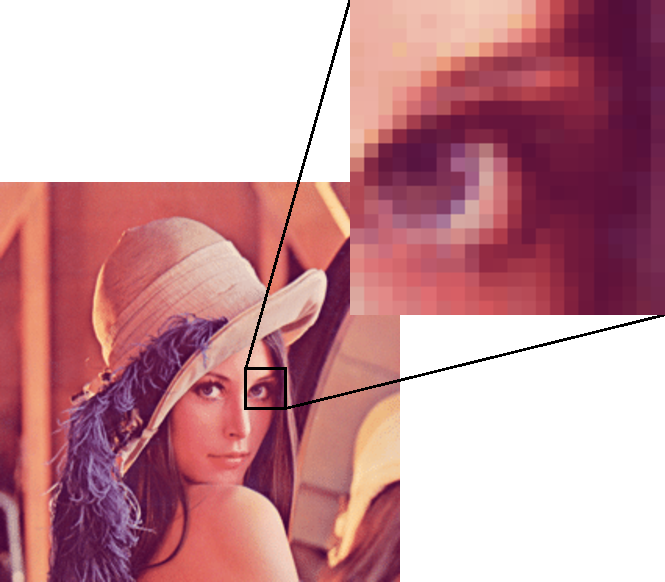
\includegraphics[width=0.5\textwidth]{images/lenaeye.pdf}
  \caption{Lena - detalhe.}\label{fig-lena-detalhe}
  \end{figure}

\end{frame} 

\begin{frame}%[allowframebreaks]
  \frametitle{Espaço necessário para armazenar uma foto}
  \begin{itemize}
  \item câmera 10 Mpixel
  \item 3 bytes por pixel (RGB)
  \item cada foto requer 30 Mbyte
  \item um cartão de memória de 2 Gbytes é capaz de armazenar 66 fotos
  \end{itemize}
\end{frame}

\begin{frame}%[allowframebreaks]
  \frametitle{Espaço necessário para armazenar um vídeo}
  \begin{itemize}
  \item 480 x 720, 30 fps
  \item 345.600 pixels por frame
  \item RGB 3 bytes por pixel
  \item 1.036.800 byte, aprox. 1 Mbyte por frame
  \item 30 frames requerem 31.104.000 bytes, aprox. 31 Mbyte por segundo
  \item um CD de 650 Mbytes é capaz de armazenar apenas 21 segundos de vídeo
  e um DVD de 4.7 GB apenas 155 segundos de vídeo.
  \end{itemize}
\end{frame}


\begin{frame}%[allowframebreaks]
  \frametitle{Dilema de compressão}
  Quando devemos parar a busca por uma \textbf{melhor} compressão?

  \vspace{1cm}
  melhor:
  \begin{itemize}
  \item menor tamanho da representação digital resultante
  \item eficiência computacional (compressão e/ou descompressão)
  \item simplicidade do algoritmo
  \end{itemize}

  \vspace{1cm}
  Qual é o limite de compressão para um determinado dado?

\end{frame} 
\note{
Modificar um algoritmo para melhorar a taxa de compressão em 1\% pode
acarretar um aumento de 10\% no tempo de execução do algoritmo e
ainda mais sobre a complexidade do programa.
}
\note{
Conjecturas\footnote{Uma conjectura é uma proposição que não é provada, mas acredita-se que seja verdadeira e não foi mostrado o contrário.}.
\vspace{2ex}

  \begin{itemize}
  \item Compressão de dados pode ser interpretada como o processo de remover complexidades (redundâncias)
  desnecessárias na informação, e desta forma, maximizando a simplicidade enquanto preserva o máximo
  possível do poder discricionário dos dados.
  \item Todo tipo de computação e racionalização formal pode ser compreendida como compressão
  de informação através do processo de identificar padrões, busca e unificação
  das instâncias destes padrões.
  \end{itemize}

}


\begin{frame}[allowframebreaks]
  \frametitle{Termos}
  \begin{description}
  \item[compressor ou codificador] é o programa que comprime os dados crus na entrada e cria uma saída de dados
  comprimida (com baixa redundância).
  \item[decompressor ou decodificador] converte os dados na direção oposta.
  \item[fluxo] é o dado a ser comprimido, armazenado como um arquivo ou transmitido.
  \item[dado não-codificado, cru, ou original] é o fluxo de dados da entrada.
  \item[dado codificado ou comprimido] é o fluxo de saída.
  \item[método de compressão não-adaptativo] é rígido e não modifica sua operação ou seus parâmetros em resposta
  aos dados em particular que estão sendo comprimidos.
  \item[método adaptativo] analisa os dados crus e modifica sua operação e/ou parâmetros de acordo com os dados em mãos.
  \item[método semi-adaptativo] utiliza 2 passagens aonde, na primeira, realiza a leitura dos dados e
  contabiliza estatísticas dos dados a serem comprimidos; na segunda passagem, realiza de fato a compressão
  utilizados parâmetros determinados na primeira varredura.
  \item[método localmente adaptativo] se adapta às condições locais do fluxo de dados e varia à medida que
  move ao longo dos dados.
  \item[compressão com perdas/sem perdas] : Para atingirem maior compressão, os métodos de compressão com perda
  perdem informação. Os métodos de compressão sem perda não admitem perder informação alguma.
  \item[Compressão em cascata] ocorre quando diferentes métodos de compressão são utilizados um em seguida do outro.
  \item[Compressçao perceptiva] ocorre quando apenas a informação imperceptível pelos nosso sentidos é removida.
  \item[Compressão simétrica] é o caso em que o compressor e descompressor utilizam basicamente o mesmo algoritmo,
  porém em direções opostas.
  \item[Complacente] é o codificador/decodificador que gera/lê de forma correta um fluxo de dados (Qualquer pessoa
  é livre para implementar seu próprio algoritmo).
  \item[Universal] é o método de compressão de dados que não depende da estatística dos dados.
  \item[Razão de Compresão] $=$ tamanho do dado de saída / tamanho do dado de entrada.
  \item[Fator de Compressão] $=$ tamanho do dado de entrada / tamanho do dado de saída $=$ (razão de compressão)$^{-1}$.
  \item[Ganho de Compressão] $= 100 \log_e $ (tamanho de referência / tamanho comprimido), aonde o tamanho de referência é o tamanho dos dados de entrada ou o tamanho do dado de saída comprimido por algum algoritmo padrão.
  \item[Erro médio quadrático (MSE) e relação sinal ruído de sinal (PSNR)] são utilizados para medir a distorção causada por uma compressão com perdas.
  \end{description}
\end{frame} 


\begin{frame}%[allowframebreaks]
  \frametitle{Termos}
  \begin{figure}[h]
  \centering
  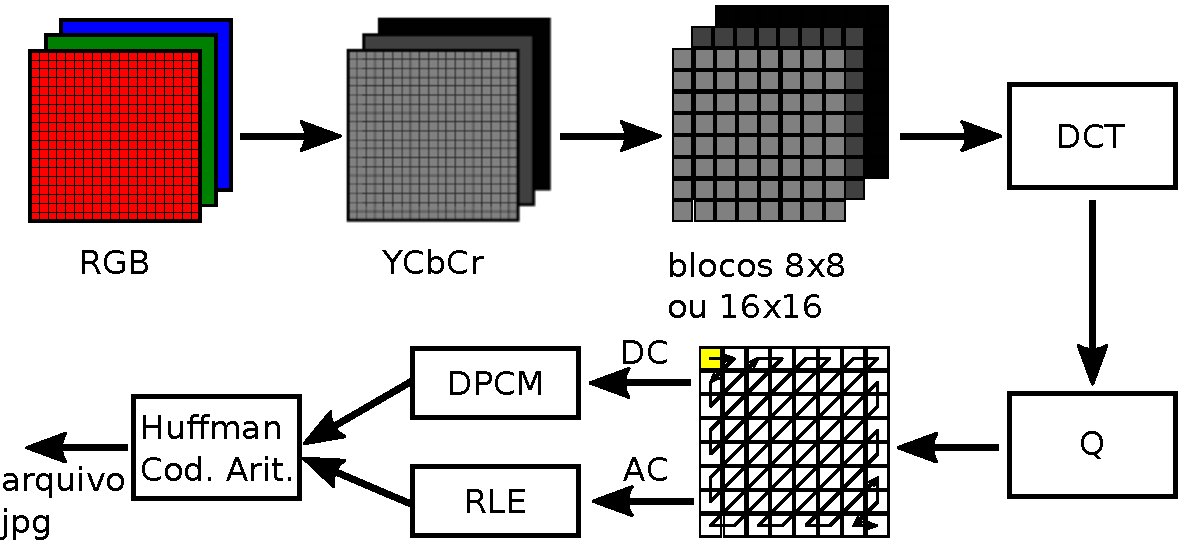
\includegraphics[width=0.8\textwidth]{images/jpegstd.pdf}
  \caption{Esquema de compressão JPEG.}\label{fig-jpegstd}
  \end{figure}
\end{frame} 

\begin{frame}%[allowframebreaks]
  \frametitle{Slides- introdução ao GNU Octave}
  \centering
  
\includegraphics[width=0.4\textwidth]{images/qrcode-octave-intro.pdf}

  \url{https://drive.google.com/open?id=1ew5fl9v_OIybsy3KdEgIvohLTcuwuru_}
\end{frame} 

\begin{frame}%[allowframebreaks]
  \frametitle{Notebook - introdução}
  \centering
  
\includegraphics[width=0.4\textwidth]{images/qrcode-jupyter-intro.pdf}

  \url{https://nbviewer.jupyter.org/github/leolca/notebooks/blob/master/aev/introducao.ipynb}
\end{frame} 

\begin{frame}%[allowframebreaks]
  \frametitle{Notebook - imagem colorida}
  \centering
  
\includegraphics[width=0.4\textwidth]{images/qrcode-jupyter-im-color.pdf}

  \url{https://nbviewer.jupyter.org/github/leolca/notebooks/blob/master/aev/introdocao_imagem_colorida.ipynb}
\end{frame} 



\subsection{Informação}
\begin{frame}%[allowframebreaks]
  \frametitle{Informação}
  O conceito de informação é amplo, sendo difícil ser contemplado em sua plenitude por qualquer definição.

  \vspace{2ex}
  \citet{shannon1948} propôs a definição de \textit{entropia} que possui
  muitas propriedades em comum o senso comum do que deve ser informação.

  \vspace{2ex}
  A informação fornecida por uma mensagem corresponde com o quão improvável é esta mensagem.

\end{frame}
\note{
O que é previsível fornece pouca ou nenhuma informação.

Quanto mais incerto, mais informação há.
}

\begin{frame}%[allowframebreaks]
  \frametitle{Informação}
  \citet{hartley1928} propõem uma medida de informação para uma variável aleatória $X$:
  \begin{equation}
    I(X) = \log_b L ,
  \end{equation}
  onde $L$ é o número de possíveis valores que $X$ pode assumir.
  Se $b=2$, a informação será medida em `bits' (nome sugerido por J.W. Tukey).
\end{frame}
\note{
  A definição de Hartley é condizente com as seguintes intuições sobre informação: 
  \begin{itemize}
  \item Dois cartões de memória devem possuir o dobro da capacidade de um cartão para
  armazenamento de informação.
  \item Dois canais de comunicação idênticos devem possuir o dobro da capacidade 
  de transmitir informação que um único canal.
  \item Um dispositivo com duas posições estáveis, como um relé ou um flip-flop,
  armazena um bit de informação. $N$ dispositivos deste tipo podem armazenar $N$ bits
  de informação, já que o número total de estados é $2^N$ e $\log_2 2^N = N$.
  \end{itemize}

  Entretanto, isto é válido apenas quando as mensagens/eventos são equiprováveis. 
  No caso extremo, note que se o cartão de memória armazena apenas zeros, ele não
  é capaz de armazenar informação alguma.
}

\begin{frame}%[allowframebreaks]
  \frametitle{Entropia}
  Suponha que existam eventos $E_k$ com probabilidade de ocorrência $p_k$. 

  \begin{itemize}
  \item Shannon: informação associada ao evento $E_k$ é dada por $I(E_k) = \log (1/p_k)$.
        \begin{itemize}
        \item Se $p_k=1$ $\rightarrow$ não há surpresa na ocorrência do evento $E_k$.
        \item Se $p_k=0$ $\rightarrow$ surpresa infinita, afinal o evento $E_k$ é impossível.
        \item $I(E_k) = - \log p(E_k)$ é a auto-informação do evento ou mensagem $E_k$.
        \end{itemize}
  \item \textbf{Sempre} utilizaremos a base $2$ para o cálculo do logaritmo, desta forma
  $\log \equiv \log_2$, a menos que seja especificado o contrário.
  \item $\ln$ é o logaritmo na base natural $e$.
  \end{itemize}
\end{frame}

\begin{frame}%[allowframebreaks]
  \frametitle{Entropia}
  \begin{itemize}
  \item Notação: $p(x) = P_X(X=x)$, a probabilidade do evento $\{X=x\}$, da v.a. $X$ assumir o valor $x$.
  \item Valor esperado da v.a. $X$: $E[X] = EX = \sum_x x p(x)$.
  \item Dada uma função $g: \mathcal{X} \rightarrow \mathbb{R}$, o valor esperado da
  v.a. $g(X)$ é $E g(X) = \sum_x g(x) p(x)$.
  \item Considere $g(x) = \log(1/p(x))$. Então $g(x)$ é a imprevisão (surpresa) de encontrar o evento $X=x$.
        Tomando o valor esperado de $g$ teremos
        \begin{equation}
        \sum_x p(x) \log \frac{1}{p(x)} ,
        \end{equation}
        ou seja, a esperança da surpresa, ou o valor esperado da imprevisão na variável aleatória $X$.
        Esta é a definição de entropia.
  \end{itemize}
\end{frame}


% entropia
\section{Entropia}
\subsection{Definição de entropia}
\begin{frame}%[allowframebreaks]
  \frametitle{Entropia}
  \begin{definition}[Entropia]\label{def-entropia}
  Dada uma variável aleatória $X$ sob um alfabeto de tamanho finito $\mathcal{X}$, a \textbf{entropia}
  da variável aleatória é dada por
  \begin{eqnarray}
  H(X) &\triangleq& E_p \log \frac{1}{p(X)} = E \log \frac{1}{p(X)} \\
        &=& \sum_{x \in \mathcal{X}} p(x) \log \frac{1}{p(x)} = - \sum_x p(x) \log p(x)
  \end{eqnarray}
  \end{definition}
  A unidade de entropia é `bits', já que utilizamos o logaritmo na base $2$ (unidade `nats' se 
  utilizar a base $e$).
\end{frame}
\note{  
  \begin{itemize}
  \item Entropia mede a grau de incerteza associado a uma distribuição.
  \item Entropia mede a desordem ou o espalhamento de uma distribuição.
  \item Entropia mede a `escolha' que a fonte tem na escolha de símbolos de acordo com uma densidade 
        (maior entropia implica em mais escolha).
  \item Vamos utilizar a seguinte convenção: $0 \log 0 = 0$.
  \end{itemize}
}

\begin{frame}%[allowframebreaks]
  \frametitle{Entropia}
  Se uma v.a. $X \sim p(x)$, então o valor esperado de uma função desta v.a., $g(X)$, é dada por
  \begin{equation}
  E[g(X)] = \sum_{x \in \mathcal{X}} p(x) g(x) .
  \end{equation}

  A entropia de $X$ pode ser interpretada como o valor esperado da v.a. $\log \frac{1}{p(X)}$,
  onde $X$ é descrita pela função massa de probabilidade $p(x)$.
  \begin{equation}
  H(X) = E \left[ \log \frac{1}{p(X)} \right] .
  \end{equation}
\end{frame}
\note{
  \begin{itemize}
  \item Entropia é uma medida da real `incerteza' média, o que é uma medida sobre toda a distribuição.
  \item Entropia mede o grau de incerteza médio ou esperado do resultado de uma distribuição de probabilidade.
  \item É uma medida de desordem ou espalhamento. Distribuições com alta entropia devem ser planas, mais
  uniformes, enquanto distribuições com baixa entropia devem possuir poucas modas (unimodal, bimodal).
  \end{itemize}
}
\note{
  \begin{figure}[h!]
  \centering
  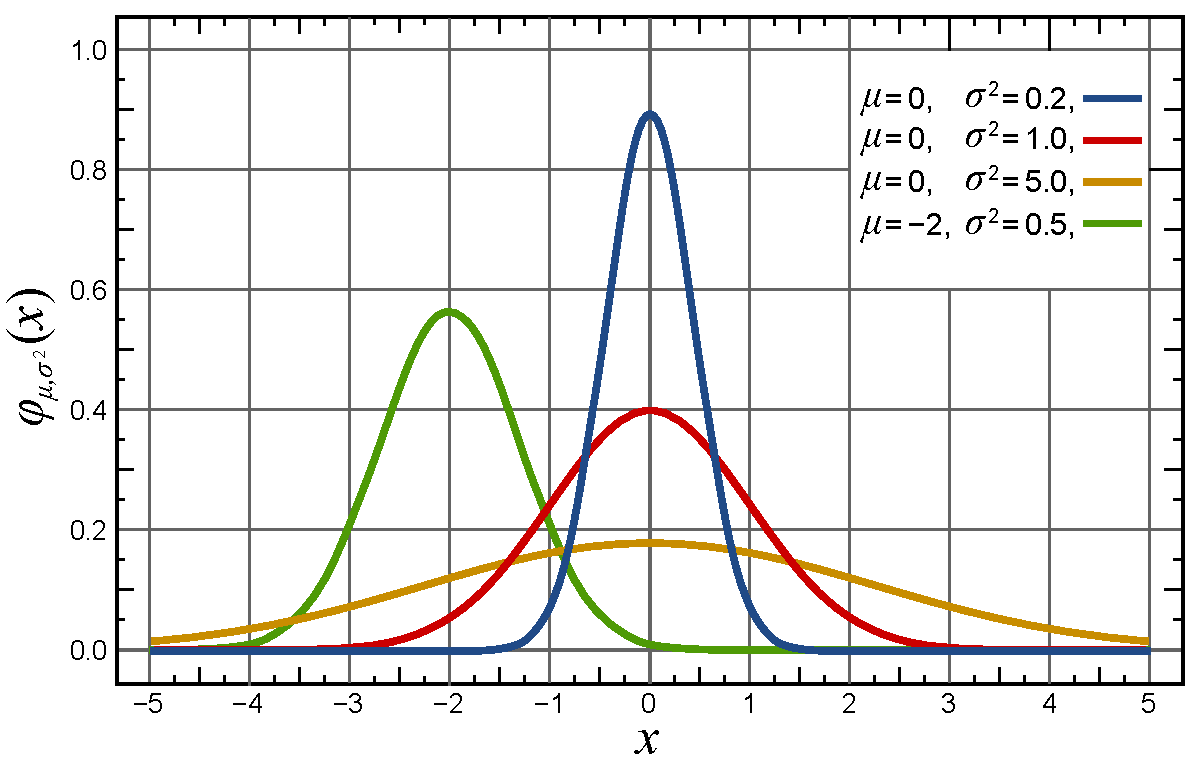
\includegraphics[width=0.4\textwidth]{images/normal_distribution.pdf}
  %\caption{.}
  \label{fig:normal_distribution}
  \end{figure}

  \begin{itemize}
  \item mais concentrado: menor entropia
  \item mais espalhado: maior entropia
  \item os valores em $x$ não importam, 
  apenas os valores das probabilidades associadas $p(x)$ importam no cálculo da entropia
  \end{itemize}
}

\begin{frame}[allowframebreaks]
  \frametitle{Escolha, Incerteza e Entropia}
  Suponha um conjunto de eventos cujas probabilidades de ocorrências sejam dadas
  por $p_1, p_2, \ldots, p_n$. É possível encontrar uma medida de quanta `escolha' 
  está envolvida na seleção de um evento ou quão incertos estamos da saída?

  Para tal medida $H(p_1, p_2, \ldots, p_n)$, é razoável requerermos as seguintes propriedades:
  \begin{enumerate}
  \item $H$ deve ser contínuo em $p_i$;
  \item Se todos os $p_i$ são iguais, $p_i=\frac{1}{n}$, então $H$ deve ser uma função
  monotonicamente crescente de $n$ (quando temos eventos equiprováveis, teremos mais incerteza
  quão maior for o número de eventos possíveis);
  \item Se for possível quebrar uma escolha em uma sequência de escolhas sucessivas,
  a medida $H$ original deve ser a soma ponderada dos valores individuais das medidas
  $H_i$ após a quebra.
  
     \begin{figure}[h!]
     \centering
     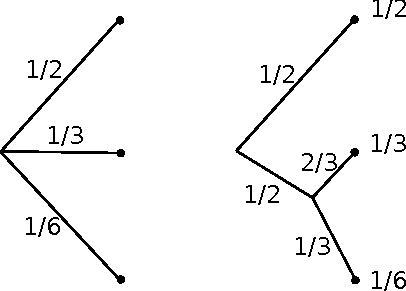
\includegraphics[width=0.3\textwidth]{images/entr-quebra.pdf}
     %\caption{Df.}
     \label{fig:entr-quebra}
     \end{figure}

  \begin{equation}
  H(\frac{1}{2},\frac{1}{3},\frac{1}{6}) = H(\frac{1}{2},\frac{1}{2}) + \frac{1}{2} H(\frac{2}{3},\frac{1}{3})
  \end{equation}
  \end{enumerate}

  A única função $H$ que satisfaz às suposições acima é da forma \cite{shannon1948}: 
  \begin{equation}\label{eq-K-entropia}
  H = - K \sum_{i=1}^{k} p(i) \log p(i) \textmd{ ,}
  \end{equation} 
  onde $K$ é uma constante positiva. 
\end{frame}




\subsection{Demonstração da equação da entropia}
\begin{frame}[allowframebreaks]
  \frametitle{Demonstração da \Cref{eq-K-entropia}}

  Nesta secção iremos apresentar a demonstração de $H=-\sum p_i \log p_i$ 
  (conforme Apêndice 2 de \citet{shannon1948}).

  Vamos definir
  \begin{equation}
  A(n) = H\left( \frac{1}{n}, \frac{1}{n}, \ldots, \frac{1}{n} \right) .
  \end{equation}

  Desejamos que uma escolha dentre $s^m$ opções igualmente prováveis possa ser decomposta como uma sequência de $m$ escolhas
  que se subdividem em $s$ possibilidades igualmente prováveis.

  \begin{figure}[h!]
  \centering
  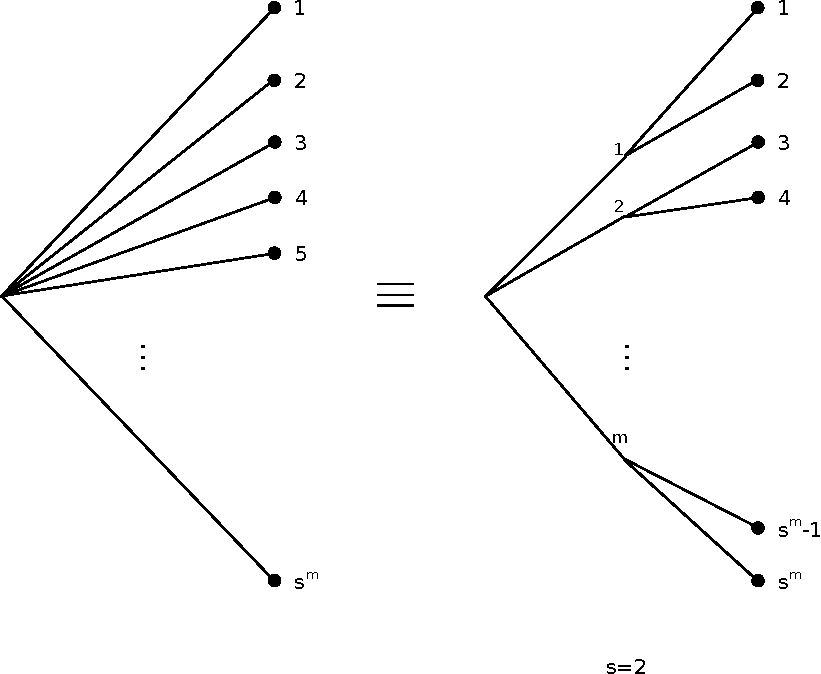
\includegraphics[width=0.5\textwidth]{images/choices.pdf}
  \caption{Exemplo de equivalência para $s=2$.}
  \label{fig:choiceseqv}
  \end{figure}

  Teremos então que
  \begin{equation}
  A(s^m) = m A(s) .
  \end{equation}
  Da mesma forma, para $t$ e $n$, teremos $A(t^n) = n A(t)$.
  Podemos tomar $n$ arbitrariamente grande e encontrar $m$ que satisfaça
  \begin{equation}
  s^m \leq t^n \leq s^{(m+1)} .
  \end{equation}
  Tomando o logaritmo\footnote{Logaritmo é uma função monótona crescente.} da expressão acima e dividindo 
  por $n \log s$ todos os termos\footnote{$n \log s$ é positivo para $n \geq 0$ e $s \geq 1$.}, teremos
  \begin{equation}
  \frac{m}{n} \leq \frac{\log t}{\log s} \leq \frac{m}{n} + \frac{1}{n} ,
  \end{equation}
  o que é equivalente a 
  \begin{equation}
  \left\vert \frac{m}{n} - \frac{\log t}{\log s} \right\vert < \epsilon ,
  \end{equation}
  onde $\epsilon$ é arbitrariamente pequeno, já que $n$ é arbitrariamente grande.

  Usando agora a propriedade desejada de monotonicidade de $A(n)$, teremos
  \begin{alignat}{3}
  A(s^m) &\leq A(t^n) &\leq A(s^{(m+1)}) \nonumber \\
  mA(s) &\leq nA(t) &\leq (m+1)A(s)
  \end{alignat}

  Dividindo a expressão acima por $nA(s)$, teremos
  \begin{equation}
  \frac{m}{n} \leq \frac{A(t)}{A(s)} \leq \frac{m}{n} + \frac{1}{n} ,
  \end{equation}
  ou, de forma equivalente,
  \begin{equation}
  \left\vert \frac{m}{n} - \frac{A(t)}{A(s)} \right\vert < \epsilon ,
  \end{equation}
  e assim, como as duas frações ($\nicefrac{\log t}{\log s}$ e $\nicefrac{A(t)}{A(s)}$) estão $\epsilon$ próximas
  de $\nicefrac{m}{n}$, podemos concluir que
  \begin{equation}
  \left\vert \frac{A(t)}{A(s)} - \frac{\log t}{\log s} \right\vert < 2\epsilon .
  \end{equation}
  Como $\epsilon$ é arbitrariamente pequeno, no limite teremos
  \begin{eqnarray}
  \frac{A(t)}{A(s)} &=& \frac{\log t}{\log s} \nonumber \\
  A(t) &=& \frac{A(s)}{\log s} \log t = K \log t ,
  \end{eqnarray}
  onde $K$ deve ser positivo, de forma que $A(n)$ seja monótona crescente.

  Suponha uma escolha com $n$ possibilidades em que as probabilidades são comensuráveis,
  $p_i = \nicefrac{n_i}{\sum n_i}$, onde $n_i$ são inteiros. De forma equivalente,
  uma escolha entre $\sum n_i$ opções pode ser expressa como uma escolha dentre $n$ opções
  com probabilidades $p_1, \ldots, p_n$, e para uma $i$-ésima dada escolha, realizar uma
  nova escolha dentre $n_i$ opções igualmente prováveis. Teremos então:
  \begin{eqnarray}
  \overbrace{ K \log \left( \sum n_i \right) }^{A\left( \sum n_i \right)} &=& H(p_1, \ldots, p_n) + \overbrace{ K \log n_i }^{A(n_i)} \nonumber \\
  K \underbrace{\left( \sum p_i \right)}_{=1} \log \left( \sum n_i \right) &=& H(p_1, \ldots, p_n) + K \underbrace{\left( \sum p_i \right)}_{=1} \log n_i .
  \end{eqnarray}  
  E assim,
  \begin{eqnarray}
  H(p_1, \ldots, p_n) &=& K\left[ \left( \sum p_i \right) \log \left( \sum n_i \right) - \left( \sum p_i \right) \log n_i \right] \nonumber \\
        &=& -K \sum p_i \log \frac{n_i}{\sum n_i} = -K \sum p_i \log p_i . \qed
  \end{eqnarray} 
\end{frame}



\subsection{Entropia - Fonte Binária}
\begin{frame}%[allowframebreaks]
  \frametitle{Entropia Binária}
  \begin{itemize}
  \item Alfabeto binário $X \in \{0,1\}$, ou $\mathcal{X} = \{0,1\}$.
  \item $p(X=1)=p=1-p(X=0)$.
  \item $H(X) = -p \log p - (1-p) \log (1-p) = H(p)$.
  \item entropia como função de $p$

  \begin{figure}[h!]
  \centering
  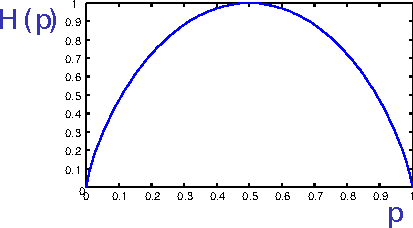
\includegraphics[width=0.5\textwidth]{images/graph_Hp.pdf}
  %\caption{.}
  \label{fig:graph_Hp}
  \end{figure}
  \end{itemize}
\end{frame}
\note{
  \begin{itemize}
  \item maior incerteza ($H=1$) quando $p=0.5$ e menor incerteza ($H=0$) quando $p=0$ ou $p=1$.
  \item note que a entropia $H(p)$ é concava em $p$.
  \end{itemize}
}


\begin{frame}%[allowframebreaks]
  \frametitle{Entropia - GNU Octave}
  \lstinputlisting[firstline=30,lastline=41,label=lst-entropy-fnc]{/home/leoca/ee/research/clscripts/entropy.m}

  \href{https://raw.githubusercontent.com/leolca/clscripts/master/entropy.m}{[download do código]}
\end{frame}

\begin{frame}%[allowframebreaks]
  \frametitle{Entropia - GNU Octave - demo}
  \lstinputlisting[firstline=43,lastline=51,label=lst-entropy-fnc]{/home/leoca/ee/research/clscripts/entropy.m}
\end{frame}

\subsection{Entropia Conjunta}
\begin{frame}%[allowframebreaks]
  \frametitle{Entropia Conjunta}
  Duas variáveis aleatórias $X$ e $Y$ possuem \textbf{entropia conjunta}
  \begin{equation}
  H(X,Y) = - \sum_{x \in \mathcal{X}} \sum_{y \in \mathcal{Y}} p(x,y) \log p(x,y) = E \log \frac{1}{p(X,Y)} .
  \end{equation}

  Generalizando para vetores $X_{1:N} = (X_1, X_2, \ldots, X_N)$
  \begin{eqnarray}
  H(X_{1:N}) &=& H(X_1, X_2, \ldots, X_N) \nonumber \\
       &=& \sum_{x_1, x_2, \ldots , x_N} p(x_1, \ldots, x_N) \log \frac{1}{p(x_1, \ldots, x_N)} \nonumber \\
       &=& E \log \frac{1}{p(X_1, \ldots, X_N)}
  \end{eqnarray}
\end{frame}



\subsection{Entropia Condicional}
\begin{frame}[allowframebreaks]
  \frametitle{Entropia Condicional}
  Dadas duas v.a. $X$ e $Y$ relacionadas por $p(x,y)$, conhecer o evento $X=x$ pode alterar a entropia de $Y$.

  \begin{itemize}
  \item Entropia condicionada a um evento $H(Y|X=x)$
     \begin{eqnarray}
     H(Y|X=x) &=& E \log \frac{1}{p(Y|X=x)} \nonumber \\
              &=& - \sum_{y \in \mathcal{Y}} p(y|x) \log p(y|x)
     \end{eqnarray}

  \item $H(Y|X=x)$ é uma função de $X$. Podemos então tomar seu valor esperado $E[H(Y|X=x)]$
  e obter a entropia condicional $H(Y|X)$.

  \item Realizando a média sobre todos os $x$, obteremos a entropia condicional $H(Y|X)$.
     \begin{eqnarray}
     H(Y|X) &=& \sum_x p(x) H(Y|X=x) \nonumber \\
        &=& - \sum_x p(x) \sum_y p(y|x) \log p(y|x) \nonumber \\
        &=& - \sum_{x,y} p(x,y) \log p(y|x) \nonumber \\
        &=& E \log \frac{1}{p(Y|X)}
     \end{eqnarray}
  \end{itemize}
\end{frame}


\subsection{Regra da Cadeia}
\begin{frame}%[allowframebreaks]
  \frametitle{Regra da Cadeia}
  \begin{theorem}[Regra da Cadeia para a Entropia]
  \begin{equation}
  H(X,Y) = H(X) + H(Y|X) = H(Y) + H(X|Y)
  \end{equation}
  \end{theorem} 
  
  \begin{proof}
  \begin{equation}
  - \log p(x,y) = - \log p(x) - \log p(y|x)
  \end{equation}
  tomando o valor esperado de ambos os lados, obtemos o resultado desejado.
  \end{proof}

  \begin{corollary}
  Se $X \independent Y$ então $H(X,Y) = H(X) + H(Y)$.
  \end{corollary}
\end{frame}


\begin{frame}%[allowframebreaks]
  \frametitle{Regra da Cadeia}
  \begin{proof}[regra da cadeia]
  \begin{eqnarray}
  H(X,Y) &=& - \sum_{x \in \mathcal{X}} \sum_{y \in \mathcal{Y}} p(x,y) \log p(x,y) = - \sum_{x \in \mathcal{X}} \sum_{y \in \mathcal{Y}} p(x,y)  \log p(y|x) p(x) \nonumber \\
        &=& - \sum_{x \in \mathcal{X}} \sum_{y \in \mathcal{Y}} p(x,y)  \log p(y|x) - \sum_{x \in \mathcal{X}} \sum_{y \in \mathcal{Y}} p(x,y)  \log p(x) \nonumber \\
        &=& H(Y|X) - \sum_{x \in \mathcal{X}} \log p(x) \sum_{y \in \mathcal{Y}} p(x,y) \nonumber \\
        &=& H(Y|X) - \sum_{x \in \mathcal{X}} \log p(x) (p(x)) \nonumber \\
        &=& H(Y|X) + H(X)
  \end{eqnarray}
  \end{proof}
\end{frame}
\note{
Exemplo Canal de Comunicação
\vspace{3ex}

   Suponha um canal de comunicação com entrada $X$ e saída $Y$.

   $H(X|Y)$ pode ser visto como a incerteza sobre $X$ (a mensagem enviada) quando 
   $Y$ (a mensagem recebida) for conhecido.

   Sem nenhuma observação no processo de comunicação através deste canal, o
   receptor não sabe nada sobre $X$ nem $Y$, assim a incerteza inicial é $H(X,Y)$.
   Quando o receptor recebe a mensagem $Y$, ele ganha uma quantidade de informação $H(Y)$.
   Assim a informação que falta sobre $X$ mesmo conhecendo $Y$ é dada por
   $H(X|Y) = H(X,Y) - H(Y)$. Esta pode ser tido como uma medida do erro na comunicação.
   A quantidade de informação que o receptor de fato ganha é $I(X;Y) = H(X) - H(X,Y)$.

}

\begin{frame}[allowframebreaks]
  \frametitle{Regra da Cadeia Generalizada}
  \begin{theorem}[Regra da Cadeia para a Entropia]
  \begin{equation}
  H(X_1, X_2, \ldots, X_N) = \sum_{i=1}^N H(X_i | X_1, X_2, \ldots, X_{i-1}) 
  \end{equation}
  \end{theorem}

  \begin{eqnarray}
  H(X_1, X_2, \ldots, X_N) &=& H(X_1) + H(X_2 | X_1) + \\
        && H(X_3 | X_1, X_2) + H(X_4 | X_1, X_2, X_3) + \cdots \nonumber
  \end{eqnarray}
  
  \framebreak
  \begin{proof}
  Utilizando a regra da cadeia da probabilidade condicional, teremos
  \begin{equation}
  p(x_1, x_2, \ldots, x_N) = \prod_{i=1}^N p(x_i | x_1, \ldots , x_{i-1}) ,
  \end{equation}
  então
  \begin{equation}
  - \log p(x_1, x_2, \ldots, x_N) = - \sum_{i=1}^N \log p(x_i | x_1, x_2, \ldots , x_{i-1}) 
  \end{equation}
  tomando o valor esperado de ambos os lados, obtemos o resultado desejado.
  \end{proof}
\end{frame}



\subsection{Propriedades da Entropia}
\begin{frame}%[allowframebreaks]
  \frametitle{Propriedades da Entropia}
  \begin{enumerate}
    \item $H$ é uma função estritamente côncava de $X$, i.e., para $0 \leq \lambda \leq 1$
      e variáveis aleatórias $X$ e $Y$
      \begin{equation}
        H(\lambda X + (1 - \lambda) Y) \geq \lambda H(X) + (1 - \lambda) H(Y)
      \end{equation}
      com igualdade sse (se e somente se) $\lambda = 0$ ou $\lambda = 1$ ou $X=Y$.
    \item $H(X) \geq 0$ com igualdade sse $p(X)$ for não nulo apenas em um ponto $x_0 \in \mathcal{X}$.
    \item $H(X) \leq \log \vert \mathcal{X} \vert$ com igualdade sse $p(X)$ for uniforme ($p \sim \frac{1}{n}$).
    \item $H(X)$ é uma função apenas das probabilidades $p(x_i)$, independente da ordem ou rótulo.
    \item $H_b(X) = (\log_b a) H_a(X)$.
  \end{enumerate}
\end{frame}


\subsection{Continuidade da Entropia}
\begin{frame}[allowframebreaks]
  \frametitle{Continuidade da Entropia}

  Todas as medidas de informação de Shannon são funções contínuas das distribuições
  conjuntas das variáveis aleatórias envolvidas.

  \begin{definition}[distância das variações]
  Seja $p$ e $q$ duas distribuições probabilísticas em um alfabeto comum $\mathcal{X}$.
  A distância das variações entre $p$ e $q$ é definida por
  \begin{equation}
  V(p,q) = \sum_{x \in \mathcal{X}} \vert p(x) - q(x) \vert .
  \end{equation}
  \end{definition} 

  Dado um alfabeto finito fixo $\mathcal{X}$, considere $\mathcal{P}_\mathcal{X}$ o
  conjunto de todas as distribuições em $\mathcal{X}$. A entropia para uma dada distribuição
  $p$ sobre o alfabeto $\mathcal{X}$ é definida por
  \begin{equation}
  H(p) = - \sum_{x \in S_p} p(x) \log p(x) ,
  \end{equation}
  onde $S_p$ denota o suporte de $p$, ou seja, $S_p \subset \mathcal{X}$.
  
  Para que $H(p)$ seja contínuo com respeito à convergência em distância das variações,
  em uma determinada distribuição $p \in \mathcal{P}_\mathcal{X}$, devemos ter que,
  para qualquer $\epsilon > 0$, existe $\delta > 0$ tal que
  \begin{equation}
  \vert H(p) - H(q) \vert < \epsilon ,
  \end{equation}
  para todo $q \in \mathcal{P}_\mathcal{X}$ satisfazendo 
  \begin{equation}
  V(p,q) < \delta ,
  \end{equation}
  ou, de forma equivalente, 
  \begin{equation}
  \lim_{p' \rightarrow p} H(p') = H\left( \lim_{p' \rightarrow p} p' \right) = H(p) ,
  \end{equation}
  onde a convergência $p' \rightarrow p$ é em distância das variações.

  Como $a \log a \rightarrow 0$ quando $a \rightarrow 0$, definimos uma função 
  $l:[0,\infty) \rightarrow \mathbb{R}$ da forma
  \begin{equation}
  l(a) = \begin{cases} 
        a\log a & \quad \text{se } a > 0 , \\
        0       & \quad \text{se } a = 0 ,
        \end{cases}
  \end{equation}
  ou seja, $l(a)$ é uma extensão contínua de $a \log a$.
  Podemos reescrever a entropia da seguinte forma
  \begin{equation}
  H(p) = - \sum_{x \in \mathcal{X}} l(p(x)) ,
  \end{equation}
  onde o somatório é tomado em todo $x \in \mathcal{X}$ ao invés de $S_p$.
  Definindo uma função $l_x: \mathcal{P}_\mathcal{X} \rightarrow \mathbb{R}$, para
  todo $x \in \mathcal{X}$, da forma 
  \begin{equation}
  l_x(p) = l(p(x)) ,
  \end{equation}
  teremos
  \begin{equation}
  H(p) = - \sum_{x \in \mathcal{X}} l_x(p) . \label{eqHsumXl}
  \end{equation}
  Evidentemente $l_x(p)$ é contínua em $p$ (com relação à convergência em 
  distância das variações). Como o somatório na Equação \ref{eqHsumXl} possui
  apenas um número finito de termos, podemos concluir que $H(p)$ é uma função
  contínua de $p$.
\end{frame}


\subsection{Limite Superior da Entropia}
\begin{frame}%[allowframebreaks]
  \frametitle{Limite superior para o Log} 
  \begin{figure}[h!]
  \centering
  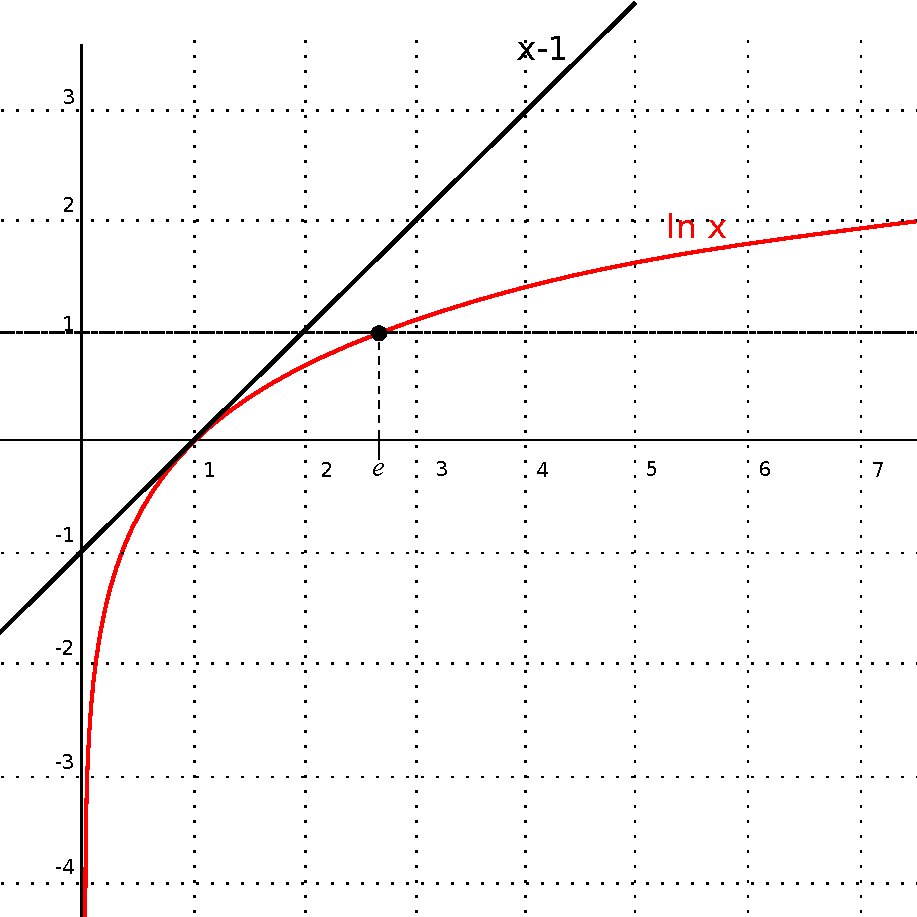
\includegraphics[width=0.4\textwidth]{images/lnx-x-1.pdf}
  %\caption{.}
  \label{fig:lnx-x-1}
  \end{figure}
  \begin{equation}
  \ln x \leq x-1
  \end{equation}
\end{frame}
\note{
$\ln x \leq x-1$, para $x \geq 1$

\begin{itemize}
\item Sabemos que para $x=1$ é verdadeiro, $0 = \ln 1 \leq 1 - 1 =0$.
\item Vamos demonstrar que $\ln x \leq x-1$, para $x \geq 1$ por contradição.
\end{itemize}
Suponha que existe $b > 1$ tal que $\ln x > x - 1$, para $x=b$.
Vamos definir $f(x) = \ln x - x + 1$, logo $f(1) = 0$ (conforme visto acima)
e $f(b) > 0$ (por hipótese).
Pelo teorema do valor médio $\exists c$, $1 < c < b$, tal que
\begin{equation}
f'(c) = \frac{f(b) - f(1)}{b - 1} = \frac{\overbrace{f(b)}^{>0}}{\underbrace{b-1}_{>0}} > 0 .
\end{equation}
Mas, $f'(x) = 1/x -1$, e assim $f'(x) < 0$ para $x>1$. Logo há uma contradição
e nossa hipótese é falsa. Teremos assim $\ln x \leq x-1$, para $x \geq 1$.

Para $x \in (0,1)$, basta seguir os mesmos passos, escolhendo um ponto 
$x=b$, tal que $0 < b < 1$. Vamos encontrar um ponto $c$ tal que $0 < b < c < 1$. 
E usar o teorema do valor médio para mostrar uma contradição na hipótese.  
}


\begin{frame}[allowframebreaks]
  \frametitle{Valor Máximo da Entropia (discreta)}
  \begin{theorem}[Limite Superior da Entropia]
  Seja $X \in \{x_1, x_2, \ldots, x_n\}$. Então $H(X) \leq \log n$, sendo a igualdade
  alcançada se e somente se $p(X=x_i) = \frac{1}{n}$ para todo $i$. 
  \end{theorem}
  \framebreak
  \begin{proof}
  Vamos mostrar que $H(X) - \log n  \leq 0$.
    \begin{eqnarray}
    H(X) - \log n &=& - \sum_x p(x) \log p(x)  - \log n \overbrace{\sum_x p(x)}^{=1} \nonumber \\
        &=& - \sum_x p(x) \log p(x) - \sum_x p(x) \log n \nonumber \\
        &=& - \sum_x p(x) \log p(x) n = \log_2 e \sum_x p(x) \ln \frac{1}{p(x) n} \nonumber \\
        &\leq& \log_2 e \sum_x p(x) \left[ \frac{1}{p(x) n} -1 \right] \nonumber
    \end{eqnarray}

   \proofbreak
    \begin{eqnarray}
    H(X) - \log n &\leq& \ldots \nonumber \\
        &=& \log_2 e \left[ \underbrace{\sum_x \frac{1}{n}}_{\sum_{x \in \mathcal{X}} \frac{1}{n} = n \frac{1}{n} = 1} - \underbrace{\sum_x p(x)}_{=1} \right] = 0
    \end{eqnarray} 
  \end{proof} 
\end{frame}


\begin{frame}%[allowframebreaks]
  \frametitle{Valor Máximo da Entropia}
  Na demonstração acima utilizamos $\ln z \leq z - 1$. A igualdade $\ln z = z-1$ se dará
  no ponto estacionário $z=1$, isto é, quando $\frac{1}{p(x) n} = 1$, ou seja,
  quando $p(x) = 1/n$, teremos assim uma distribuição uniforme.

  \vspace{1cm}
  Se tivermos $p_i = 1/n$, então
  \begin{equation}
  - \sum_i p_i \log p_i = - \sum_i \frac{1}{n} \log \frac{1}{n} = - \log \frac{1}{n} = \log n .
  \end{equation}
  Podemos mostrar (através da concavidade da entropia) que este é o único conjunto de valores com esta propriedade.

  \begin{itemize}
  \item Entropia aumenta quando a distribuição se torna mais uniforme.
  \end{itemize}
\end{frame}

\begin{frame}[allowframebreaks]
  \frametitle{Valor Máximo da Entropia}
  Outra demonstração...

  \begin{proof}
    Considere $X \in \mathcal{X} = \{x_1, x_2, \ldots, x_n\}$ com probabilidades
    $p=\{p_1, p_2, \ldots, p_n\}$, respectivamente. A entropia de $X$ é dada por
    \begin{eqnarray}\label{eq-dem-entr-max2}
    H(X) &=& - \sum_{i=1}^n p_i \log p_i \nonumber \\
        &=& - \sum_{i=1}^{n-1} p_i \log p_i - p_n \log p_n \nonumber \\
        &=& - \left( \frac{1}{\ln 2} \right) \left[ \sum_{i=1}^{n-1} p_i \ln p_i + p_n \ln p_n \right] .
    \end{eqnarray}
    \proofbreak

    Da mesma forma, podemos expressa $p_n$ da seguinte maneira
    \begin{equation}\label{eq-pn-n-1}
    p_n = 1 - \sum_{i=1}^{n-1} p_i .
    \end{equation}
    Utilizando \ref{eq-pn-n-1} em \ref{eq-dem-entr-max2}, podemos expressar
    a entropia $H(X)$ como uma função de $n-1$ probabilidades $p_i$. O máximo
    será dado quando a seguinte condição ocorrer
    \begin{equation}\label{eq:condmaxent}
    \frac{\partial H(X)}{ \partial p_k } = 0 \textmd{ \ for \ } k = 1, \ldots, n-1 \textmd{ .}
    \end{equation}

    \proofbreak
    Teremos então
    \begin{eqnarray}\label{ea:dHeqz}
        0 = \frac{\partial H(X)}{ \partial p_k } &=&  - \left( \frac{1}{\ln 2} \right) \frac{\partial}{ \partial p_k } \left[ \sum_{i=1}^{n-1} p_i \ln p_i  + p_n \ln p_n \right] \nonumber \\
        &=& - \left( \frac{1}{\ln 2} \right) \left[ \ln p_k + 1 + (\ln p_n + 1) \frac{\partial p_n}{ \partial p_k }  \right] \nonumber \\
        &=& - \left( \frac{1}{\ln 2} \right) \left[ \ln p_k + 1 - (\ln p_n + 1) \right] ,
    \end{eqnarray}
    onde utilizamos a Equação \ref{eq-pn-n-1}, que nos fornece $\partial p_n / \partial p_k = -1$.

    \proofbreak
    A Equação \ref{ea:dHeqz} mostra que devemos encontrar $\ln p_k = \ln p_n$ para cada $k=1,\ldots,n-1$.
    Todas as $n-1$ equações serão satisfeitas quando todas as probabilidades $p_k$ forem iguais a $1/n$.

    \proofbreak
    Devemos agora calcular a derivada segunda para mostrar que o extremo que achamos é de fato um máximo.
    \begin{eqnarray}\label{ea:d2Heqz}
        \frac{\partial^2 H(X)}{ \partial p_k^2 } &=& - \left( \frac{1}{\ln 2} \right) \frac{\partial}{ \partial p_k } \left[ \ln p_k - \ln p_n \right] \nonumber \\
           &=& - \left( \frac{1}{\ln 2} \right) \left[ \frac{1}{p_k} + \frac{1}{p_n} \right] \leq 0 \textmd{ ,}
    \end{eqnarray}
    já que as probabilidades são valores positivos. Escolhendo então $p_k = 1/n$, teremos a entropia máxima.

  \end{proof}
\end{frame}



\subsection{Subdividindo em partes}
\begin{frame}[allowframebreaks]
  \frametitle{Subdividindo a entropia em partes}
  A entropia deve permanecer inalterada, mesmo quando subdividimos as escolhas em partes.
 
  \begin{example}[Exemplo simples]
  Suponha uma v.a. $X$ com alfabeto $\mathcal{X} = \{x_1, x_2, x_3, x_4 \}$
  e distribuição $q = (q_1. q_2, q_3, q_4)$.

  A entropia associada a esta variável aleatória é dada por
  \begin{eqnarray}
  H(X) &=& H(q_1, q_2, q_3, q_4) \nonumber \\
        &=& - \sum_{i=1}^{4} q_i \log q_i \nonumber \\
        &=& - q_1 \log q_1 - q_2 \log q_2 - q_3 \log q_3  - q_4 \log q_4 .
  \end{eqnarray}

  \examplebreak

  Se dividirmos a escolha na determinação de $X$ em duas escolhas sucessivas,
  conforme ilustrado na figura abaixo, poderemos então escrever
  \begin{equation}
  H(q_1, q_2, q_3, q_4) = H(p_1, p_2) + p_1 H(p_{1,1}, p_{1,2}) + p_2 H(p_{2,1},p_{2,2}) .
  \end{equation}

        \begin{figure}[h!]
        \centering
        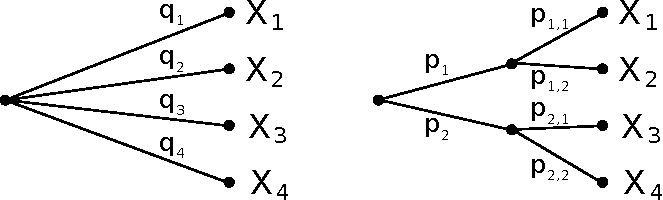
\includegraphics[width=0.5\textwidth]{images/choices4.pdf}
        \label{fig:choices4}
        \end{figure}

  \examplebreak
  \vspace{-2ex}
  \begin{eqnarray}
  H(X)  &=& - q_1 \log q_1 - q_2 \log q_2 - q_3 \log q_3  - q_4 \log q_4 \nonumber \\
        &=& - p_1 p_{1,1} \log p_1 p_{1,1} - p_1 p_{1,2} \log p_1 p_{1,2} - p_2 p_{2,1} \log p_2 p_{2,1} - p_2 p_{2,2} \log p_2 p_{2,2} \nonumber \\
        &=& - p_1 p_{1,1} \log p_1 - p_1 p_{1,1} \log p_{1,1} - p_1 p_{1,2} \log p_1 - p_1 p_{1,2} \log p_{1,2} ... \nonumber \\
        && - p_2 p_{2,1} \log p_2 - p_2 p_{2,1} \log p_{2,1} - p_2 p_{2,2} \log p_2  - p_2 p_{2,2} \log p_{2,2} \nonumber \\
        &=& - p_1 \log p_1 \left( p_{1,1} + p_{1,2} \right) - p_2 \log p_2 \left( p_{2,1} + p_{2,2} \right) ... \nonumber \\
        && + p_1 \left( - p_{1,1} \log p_{1,1} - p_{1,2} \log p_{1,2} \right) ... \nonumber \\
        && + p_2 \left( - p_{2,1} \log p_{2,1} - p_{2,2} \log p_{2,2} \right)  \nonumber \\
        &=& H(p_1, p_2) + p_1 H(p_{1,1}, p_{1,2}) + p_2 H(p_{2,1}, p_{2,2}) 
  \end{eqnarray} 
  \end{example}

  \framebreak

        \begin{figure}[h!]
        \centering
        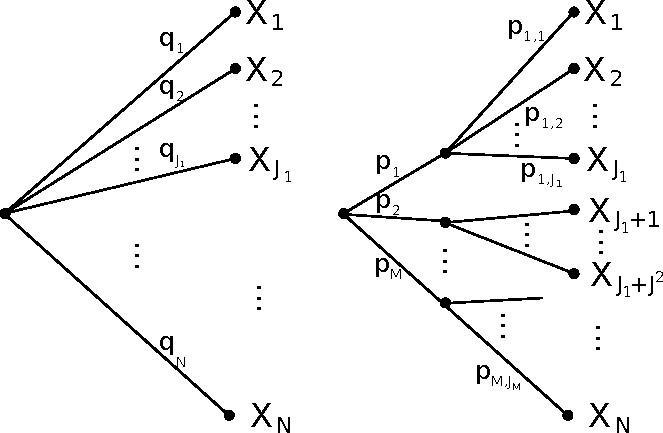
\includegraphics[width=0.5\textwidth]{images/choicesM.pdf}
        \label{fig:choicesM}
        \end{figure} 

  De forma geral, como $q_n = p_m p_{m,j}$, teremos
  \begin{eqnarray}
  H(X) &=& - \sum_{n=1}^N q_n \log q_n = - \sum_{m=1}^M \sum_{j=1}^{J_m} p_m p_{m,j} \log p_m p_{m,j} \nonumber \\
        &=& - \sum_{m=1}^M \sum_{j=1}^{J_m} \left( p_m p_{m,j} \log p_m + p_m p_{m,j} \log p_{m,j} \right) \nonumber \\
        &=& - \sum_{m=1}^M \sum_{j=1}^{J_m} p_m p_{m,j} \log p_m - \sum_{m=1}^M \sum_{j=1}^{J_m} p_m p_{m,j} \log p_{m,j} \nonumber \\
        &=& - \sum_{m=1}^M p_m \log p_m \left( \sum_{j=1}^{J_m} p_{m,j} \right) - \sum_{m=1}^M p_m \sum_{j=1}^{J_m} p_{m,j} \log p_{m,j} \nonumber \\
        &=& H(p_1, \ldots, p_M) + \sum_{m=1}^M p_m H(p_{m,1}, \ldots, p_{m,J_m}) .
  \end{eqnarray}
  
\end{frame}

\subsection{Embaralhar}
\begin{frame}%[allowframebreaks]
  \frametitle{Embaralhar}
  \begin{itemize}
  \item Suponha que $X$ seja uma v.a. indicando as posições de cartas (i.e. $X=x$ representa
  um conjunto de posições, uma determinada configuração).
  \item Seja $T$ uma operação de embaralhamento independente, i.e. $T \independent X$.
  \item Então $H(TX) \geq H(X)$.
  \begin{eqnarray}
  H(TX) &\geq& H(TX|T) \nonumber \\
        && \parbox[c]{0.7\linewidth}{\small onde utilizamos que condicionar não pode aumentar a entropia, como veremos adiante} \nonumber \\
        &=& H(T^{-1}TX|T) \nonumber \\
        && \parbox[c]{0.7\linewidth}{\small como $T$ é conhecido, aplicá-lo novamente ou seu inverso não altera a entropia} \nonumber \\
        &=& H(X|T) = H(X) \\
        && \parbox[c]{0.7\linewidth}{\small onde utilizamos que $T \independent X$} \nonumber
  \end{eqnarray}

%  \begin{equation}
%  H(TX) \geq H(TX|T) = H(T^{-1}TX|T) = H(X|T) = H(X)
%  \end{equation}
%  (onde utilizamos que condicionar não pode aumentar a entropia, como veremos adiante).
  \end{itemize}
\end{frame} 

\begin{frame}%[allowframebreaks]
  \frametitle{Permutação}
  O que ocorre se permutarmos as probabilidades?
  
  Seja $p=(p_1, p_2, \ldots, p_n)$, uma distribuição discreta de probabilidade e
  $\sigma = (\sigma_1, \sigma_2, \ldots, \sigma_n)$ uma permutação de $1, 2, \ldots, n$.
  
  Considere $p_\sigma = (p_{\sigma_1}, p_{\sigma_2}, \ldots, p_{\sigma_n} )$ uma permutação
  da distribuição $p$.

  Quem será maior? $H(p)$ ou $H(p_\sigma)$?

  %\pause
  \begin{equation}
  H(p) = - \sum_i p_i \log p_i = - \sum_j p_{\sigma_j} \log p_{\sigma_j} = H(p_\sigma)  .
  \end{equation}
\end{frame}

\subsection{Sumário}
\begin{frame}%[allowframebreaks]
  \frametitle{Sumário}
  Definição de Entropia
  \begin{equation}
  H(X) = - \sum_x p(x) \log p(x)
  \end{equation}

  Entropia Conjunta
  \begin{equation}
  H(X,Y) = - \sum_{x,y} p(x,y) \log p(x,y)
  \end{equation}

  Entropia Condicional
  \begin{equation}
  H(Y|X) = - \sum_{x,y} p(x,y) \log p(y|x)
  \end{equation}

  Regra da Cadeia
  \begin{equation}
  H(X,Y) = H(X) + H(Y|X) = H(Y) + H(X|Y)
  \end{equation}

  Limites da Entropia
  \begin{equation}
  0 \leq H(X) \leq \log n , \textmd{onde } n \textmd{ é o tamanho do alfabeto de } X.
  \end{equation}

\end{frame}


\subsection{Entropia do Jogo de Adivinhação}

\begin{frame}%[allowframebreaks]
  \frametitle{Entropia do Jogo de Adivinhação}
  Qual é a melhor estratégia para adivinhar o valor de uma variável aleatória
  com perguntas sim/não do tipo ``$X\in S$?'', para algum conjunto $S \subseteq D_X$
  (domínio da v.a. $X$).

  \begin{exampleblock}{Exemplo}
    Seja $X \in D_X = \{x_1, x_2, x_3, x_4, x_5\}$ com probabilidades
        \begin{tabular}{ c | c c c c c}
          $x$    & $x_1$ & $x_2$ & $x_3$ & $x_4$ & $x_5$ \\ \hline
          $p(x)$ & 0.3   & 0.2   & 0.2   & 0.15  & 0.15 \\
        \end{tabular}

    Considere a seguinte estratégia: 
    \begin{inlineenumerate}
        \item $X = x_5$? 
        \item $X = x_4$?
        \item $X = x_3$?
        \item $X = x_2$?
        \item $X = x_1$?
    \end{inlineenumerate}

    Desta forma faremos 5 perguntas 30\% das vezes, 4 perguntas 20\% das vezes, etc.

    O número médio de perguntas é:
    $(0.3, 0.2, 0.2, 0.15, 0.15) \cdot (5,4,3,2,1)^\intercal = 3.35$.

    Se invertermos a ordem das perguntas teremos:
    $(0.3, 0.2, 0.2, 0.15, 0.15) \cdot (1,2,3,4,5)^\intercal = 2.65$.

    Existe uma estratégia melhor?
  \end{exampleblock}
\end{frame}

\begin{frame}%[allowframebreaks]
  \frametitle{Entropia do Jogo de Adivinhação}

  Considere a estratégia ilustrada abaixo.
  \begin{figure}[h!]
  \centering
  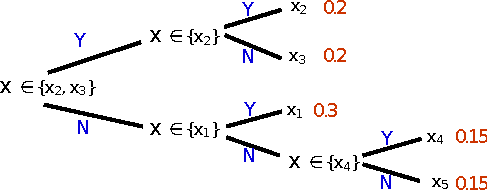
\includegraphics[width=0.75\textwidth]{images/ex-jogo-ad.pdf}
  %\caption{.}
  \label{fig:ex-jogo-ad}
  \end{figure} 

  O número médio de perguntas será:
  $2(0.2 + 0.2 + 0.3) + 3 (0.15 + 0.15) = 2.3$

  Note que $H(X) = 2.271$.

  O número médio de perguntas é sempre $\geq H(X)$.
\end{frame}

\begin{frame}%[allowframebreaks]
  \frametitle{Entropia do Jogo de Adivinhação}
  Vamos analisar a melhor e a pior estratégias, vistas anteriormente,
  com relação à forma como elas dividem a distribuição.

  \begin{itemize}
  \item pior estratégia: $X = x_5$?
 
  Divide a distribuição em dois grupos ($X=x_5$ e $X \neq x_5$), com probabilidades
  $p(X=x_5) = 0.15$, $p(X\neq x_5)=0.85$, e a entropia será $H(0.15 , 0.85) = 0.6098$.

  \item melhor estratégia: $X\in\{x_2,x_3\}$?
  
  $p(X\in\{x_2,x_3\})=0.4$, $p(X\notin\{x_2,x_3\})=0.6$, $H(0.4, 0.6)=0.971$.

  \item De forma geral, é melhor realizar primeiro perguntas que, analisadas como
  variáveis aleatórias, possuem maior entropia (algoritmo guloso).

  \item Note a relação com $H(Y|X) + H(X) = H(X,Y)$. Se fizermos uma pergunta com
  $H(X)$ grande, a entropia residual $H(Y|X)$ fica menor.
  \end{itemize}
\end{frame}
\note{
  Veremos adiante que o algoritmo guloso não é ótimo (entropia mínima).
}




\subsection{Informação Mútua}
\begin{frame}%[allowframebreaks]
  \frametitle{Intuição sobre Informação Mútua}
  \begin{itemize}
  \item Dadas duas variáveis aleatórias $X$ e $Y$, quanta informação uma possui sobre a outra?
  \item Conhecendo $X$, quanto sabemos sobre $Y$? Conhecendo $Y$, quanto sabemos sobre $X$?
  \item Se as v.a.s são independentes, $X \independent Y$, então conhecer $X$ não nos diz nada sobre
  $Y$ e vice-versa.
  \item Como temos uma medida de informação em uma fonte aleatória, $H(X)$, podemos quantificar
  quanta informação variáveis aleatórias possuem uma sobre as outras. Isto é chamado de 
  \underline{informação mútua}.
  \end{itemize}
\end{frame}

\begin{frame}%[allowframebreaks]
  \frametitle{Informação Mútua de Evento}
  Dado o evento $\{X=x, Y=y\}$, podemos nos perguntar sobre qual é a informação fornecida
  pelo evento $x$ dado o fato de que o evento $y$ ocorreu. Isto pode ser quantificado da seguinte forma:
  \begin{equation}
  I(x;y) = \log \frac{p(x|y)}{p(x)} = \underbrace{\log \frac{1}{p(x)}}_{A} - \underbrace{\log \frac{1}{p(x|y)}}_{B}
  \end{equation}
  
  \begin{itemize}
  \item Primeiro termo $A$: surpresa de que $x$ ocorreu.
  \item Segundo termo $B$: surpresa de que $x$ ocorreu dado que $y$ ocorreu.
  \item Diferença: diferença entre as duas surpresas, quanto mudou na surpresa de quando
  não sabíamos $y$ para quando passamos a saber $y$.
  \end{itemize}

  Note que $p(x|x)=1$, então $I(x;x) = \log 1/p(x) - \log 1 = \log 1/p(x) = I(x)$, então
  $I(x)$ pode ser visto como uma forma de `auto-informação'.
\end{frame}

\begin{frame}%[allowframebreaks]
  \frametitle{Informação Mútua}
  Informação Mútua é a quantidade média de informação que uma variável aleatória 
  $X$ possui sobre outra v.a. $Y$ e vice-versa.

  \begin{definition}[Informação Mútua]\label{def-inf-mut}
    \begin{eqnarray}
    I(X;Y) &=& E_{p(x,y)} \log \frac{p(x|y)}{p(x)} = E_{p(x,y)} \log \frac{p(x|y)p(y)}{p(x)p(y)} \nonumber \\
        &=& E_{p(x,y)} \log \frac{p(x,y)}{p(x)p(y)} = \sum_{x,y} p(x,y) \log \frac{p(x,y)}{p(x)p(y)}
    \end{eqnarray}
  \end{definition}
\end{frame}

\begin{frame}%[allowframebreaks]
  \frametitle{Informação Mútua e Entropia}
  \begin{proposition}
    \begin{equation}
        I(X;Y) = H(X) - H(X|Y)
    \end{equation}
  \end{proposition}
  \begin{proof}
    \vspace{-0.3cm}
    \begin{eqnarray} 
        I(X;Y)  &=& E \log \frac{p(x|y)}{p(x)} \nonumber \\
                &=& E \log \frac{1}{p(x)} - E \log \frac{1}{p(x|y)} \nonumber \\
                &=& H(X) - H(X|Y)
    \end{eqnarray}
  \end{proof}

  \begin{itemize}
  \item Por simetria, temos que $I(X;Y) = H(Y) - H(Y|X)$.
  \item Como $H(X) \geq 0$ e $H(X|Y) \geq 0$, teremos $I(X;Y) \leq \min (H(X),H(Y))$.
  \end{itemize}
\end{frame}

\begin{frame}%[allowframebreaks]
  \frametitle{Informação Mútua e Entropia}
  \begin{itemize}
  \item Regra da Cadeia da Entropia: $H(X,Y) = H(X) + H(Y|X)$.
  \item Informação Mútua: $I(X;Y) = H(X) - H(X|Y)$.
  \item Teremos então: 
        \begin{equation}
        I(X;Y) = H(X) + H(Y) - H(X,Y)
        \end{equation}
  \end{itemize}

   No próximo slide representamos estas grandezas através de um diagrama.
   As áreas utilizadas não representam conjuntos no sentido comum, mas
   representam `grau de informação' e as intersecções correspondem a
   sobreposição de informação. Isto é, a interseção consiste em informação
   fornecida por $X$ e $Y$.
\end{frame}

\begin{frame}%[allowframebreaks]
  \frametitle{Informação Mútua e Entropia - Diagrama}

  \begin{figure}[h!]
  \centering
  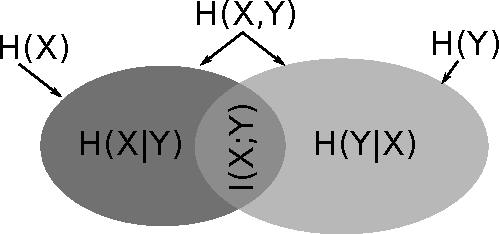
\includegraphics[width=0.75\textwidth]{images/info-set.pdf}
  %\caption{.}
  \label{fig:info-set}
  \end{figure}

\end{frame}

\subsection{Divergência de Kullbach-Leibler}
\begin{frame}%[allowframebreaks]
  \frametitle{Divergência de Kullbach-Leibler}
  A divergência de Kullbach-Leibler é uma relação fundamental entre duas 
  distribuições probabilísticas sobre um mesmo alfabeto, $p=(p_1, \ldots, p_n)$
  e $q=(q_1, \ldots , q_n)$. Esta divergência possui relação importante com a
  entropia e a informação mútua. 

  \vspace{1cm}
  Como podemos medir a `distância' entre duas distribuições $p$ e $q$ de forma útil?
  Poderíamos utilizar $D(p,q) = \sum_{i=1}^n (p_i - q_i)^2$, mas gostaríamos de ter
  uma medida de `distância de informação', isto é, uma distância que nos dê o custo
  incorrido pelo erro de considerar que uma distribuição é $q$ sendo que na realidade
  ela é $p$. Veremos que isto está ligado à insuficiência na compressão. 
  A Divergência de Kullbach-Leibler, definida a seguir, satisfaz estas ideias.
\end{frame}

\begin{frame}[allowframebreaks]
  \frametitle{Distância}
  \begin{definition}[distância]
  Seja $S$ um conjunto. Uma função $d: S \times S \rightarrow \mathbb{R}$ é chamada \textbf{distância} em $S$
  se, para todo $x,y \in S$, tivermos:
  \begin{itemize}
  \item $d(x,y) \geq 0$ (não-negatividade)
  \item $d(x,y) = d(y,x)$ (simetria)
  \item $d(x,x) = 0$ (reflexividade)
  \end{itemize}
  \end{definition}

  \framebreak
  \begin{definition}[métrica]
  Seja $S$ um conjunto. Uma função $d: S \times S \rightarrow \mathbb{R}$ é chamada \textbf{métrica} em $S$
  se, para todo $x,y \in S$, tivermos:
  \begin{itemize}
  \item $d(x,y) \geq 0$ (não-negatividade)
  \item $d(x,y) = 0$ se e somente se $x=y$ (identidade dos indiscerníveis)
  \item $d(x,y) = d(y,x)$ (simetria)
  \item $d(x,y) + d(y,z) \geq d(x,z)$ (desigualdade triangular)
  \end{itemize}
  \end{definition}
\end{frame}
\note{
Teremos uma semi-métrica se substituirmos a identidade dos indiscerníveis pela reflexividade.
}

\begin{frame}%[allowframebreaks]
  \frametitle{Diferentes formas de medir `distância' entre distribuições}

  \begin{description}
  \item[divergência de Kullback-Leibler:] $D_\mathrm{KL}(p \parallel q) = \sum p(x)\ln\left( \frac{p(x)}{q(x)}\right) $;
  \item[distância de Hellinger:] $H^2(p,\, q) = 2 \sum \Big( \sqrt{p(x)} - \sqrt{q(x)}\, \Big)^2 $;
  \item[divergência de Jeffreys:] $D_J(p \parallel q) = \sum (p(x) - q(x))\big( \ln p(x) - \ln q(x) \big) $;
  \item[divergência $\alpha$ de Chernoff:] $D^{(\alpha)}(p \parallel q) = \frac{4}{1-\alpha^2}\bigg(1 - \sum p(x)^\frac{1-\alpha}{2} q(x)^\frac{1+\alpha}{2}  \bigg) $;
  \item[divergência exponencial:] $D_e(p \parallel q) = \sum p(x)\big( \ln p(x) - \ln q(x) \big)^2$;
  \item[divergência de Kagan:] $D_{\chi^2}(p \parallel q) = \frac12 \sum \frac{(p(x) - q(x))^2}{p(x)}$;
  \item[divergência K:] $D_{\mathrm{K}}(p \parallel q) = \sum (p(x) - q(x)) \log(p(x)/q(x))$;
  \item[divergência de Jensen-Shannon:] $D_{\mathrm{JS}}(p \parallel q) = \tfrac{1}{2} D_{\mathrm{KL}} \left (p \parallel m \right ) + \tfrac{1}{2} D_{\mathrm{KL}}\left (q \parallel m \right )\, \!$, onde $m = \tfrac{1}{2}(p+q)$.
  \end{description}
\end{frame}

\begin{frame}%[allowframebreaks]
  \frametitle{Divergência de Kullbach-Leibler (Entropia relativa)}
  Sejam dadas duas distribuições, $p(x)$ e $q(x)$ sobre o mesmo alfabeto,
  $p(x) = P_p (X=x)$ e $q(x) = P_q (X=x)$, a divergência de KL é definida por

  \begin{definition}[Divergência de Kullbach-Leibler (entropia relativa)]
  \begin{equation}
  D(p||q) \triangleq \sum_x p(x) \log \frac{p(x)}{q(x)}
  \end{equation}
  \end{definition}
  Esta divergência pode ser vista como o valor esperado do logaritmo da razão das possibilidades, 
  ponderado por $p$, ou seja, $E_p \log p/q$, ou ainda, o valor esperado da diferença dos 
  logaritmos, $D(p||q) = E_p \left( \log p(x) - \log q(x) \right)$. Fornece a ideia do custo adicional
  (em bits) em se considerar uma distribuição $q$ quando a real distribuição subjacente é $p$.

  Note que a divergência de KL, em geral, não é simétrica, ou seja,
  $D(p||q) \neq D(q||p)$.

\end{frame}
\note{
  Utilizando argumentos de limite e continuidade, mostra-se que $0 \log 0 = 0$
  e $p \log (p/0) = \infty$. Fazendo estas suposições, teremos
  $D(p||q) \leq \infty$.

  A divergência de KL é uma função dos valores de probabilidade e não dos
  valores que a variável aleatória assume (assim como a entropia e a informação mútua).

  \vspace{3em}

A razão de chances ou razão de possibilidades (em inglês: \textit{odds ratio})
é definida como a razão entre a chance de um evento ocorrer em um grupo e a chance de ocorrer em outro grupo.
}
\note{
(Wikipedia)
In statistics, the odds ratio (usually abbreviated "OR") is one of three main ways 
to quantify how strongly the presence or absence of property A is associated with 
the presence or absence of property B in a given population. If each individual in 
a population either does or does not have a property "A", (e.g. "high blood pressure"), 
and also either does or does not have a property "B" (e.g. "moderate alcohol consumption") 
where both properties are appropriately defined, then a ratio can be formed which 
quantitatively describes the association between the presence/absence of "A" 
(high blood pressure) and the presence/absence of "B" (moderate alcohol consumption) 
for individuals in the population. 
}
\note{
This ratio is the odds ratio (OR) and can be computed 
following these steps:
\begin{enumerate}
\item For a given individual that has "B" compute the odds that the same individual has "A"
\item For a given individual that does not have "B" compute the odds that the same individual has "A"
\item Divide the odds from step 1 by the odds from step 2 to obtain the odds ratio (OR).
The term "individual" in this usage does not have to refer to a human being, as 
a statistical population can measure any set of entities, whether living or inanimate.
\end{enumerate}
\url{http://en.wikipedia.org/wiki/Odds_ratio}
}

\begin{frame}%[allowframebreaks]
  \frametitle{Exemplo}
  Seja $\mathcal{X} = \{1,0\}$ e considere duas distribuições $p$ e $q$ em $\mathcal{X}$.
  Seja $p(0)=1-r$, $p(1)=r$, e seja $q(0)=1-s$ e $q(1)=s$. Então
  \begin{equation}
  D(p||q) = (1-r) \log \frac{1-r}{1-s} + r \log \frac{r}{s}
  \end{equation}
  e
  \begin{equation}
  D(q||p) = (1-s) \log \frac{1-s}{1-r} + s \log \frac{s}{r} .
  \end{equation}
  Se $r=s$, então $D(p||q)=D(q||p)=0$. Se $r=\frac{1}{2}$ e $s=\frac{1}{4}$, 
  \begin{equation}
  D(p||q) = \frac{1}{2} \log \frac{1/2}{3/4} + \frac{1}{2} \log \frac{1/2}{1/4} = 1 - \frac{1}{2} \log 3 = 0.2075 \text{bits.}
  \end{equation}
  \begin{equation}
  D(q||p) = \frac{3}{4} \log \frac{3/4}{1/2} + \frac{1}{4} \log \frac{1/4}{1/2} = \frac{3}{4} \log 3 - 1 = 0.1887 \text{bits.}
  \end{equation}

   Note que, em geral, $D(p||q) \neq D(q||p)$.
\end{frame}

\begin{frame}%[allowframebreaks]
  \frametitle{Generalização da divergência de KL}
  A divergência de KL pode ser generalizada para vetores de variáveis aleatórias.

  Seja $p(x_1, \ldots, x_N)$ e $q(x_1, \ldots, x_N)$ duas distribuições sobre o vetor
  $(x_1, x_2, \ldots , x_N)$. A divergência de KL entre $p$ e $q$ é definida por
  \begin{equation}
  D(p||q) = \sum_{x_1, \ldots, x_N} p(x_1, \ldots, x_N) \log \frac{p(x_1, \ldots, x_N)}{q(x_1, \ldots, x_N)}
  \end{equation}
\end{frame}

\begin{frame}[allowframebreaks]
  \frametitle{Divergência de KL e Informação Mútua}
  Seja $\mu_1(x,y) = p(x,y)$ (distribuição conjunta) e $\mu_2(x,y)=p(x)p(y)$ (produto das marginais) 
  com $p(x)=\sum_y p(x,y)$ e $p(y)=\sum_x p(x,y)$, então
  \begin{eqnarray}
  D(\mu_1 || \mu_2) &=& \sum_{x,y} \mu_1(x,y) \log \frac{\mu_1(x,y)}{\mu_2(x,y)} \nonumber \\
                &=& \sum_{x,y} p(x,y) \log \frac{p(x,y)}{p(x)p(y)} = I(X;Y) .
  \end{eqnarray}
  A informação mútua é a distância entre a distribuição conjunta em $X$ e $Y$ e o produto
  das distribuições marginais em $X$ e $Y$.

  Se as v.a.s são independentes, teremos $p(x,y)=p(x)p(y)$ e por conseguinte a divergência será nula,
  a informação mútua entre $X$ e $Y$ será zero.

  A informação mútua é o erro em se assumir independência entre as v.a.s.

  \framebreak
  O produto das distribuições marginais $p(x)p(y)$, onde $p(x)=\sum_y p(x,y)$ e $p(y)=\sum_x p(x,y)$,
  é uma projeção da distribuição conjunta $p(x,y)$ sobre o conjunto das distribuições independentes.
  I.e.,
  \begin{equation}
  p(x)p(y) = \argmin_{p'(x,y) \backslash p'(x,y)=p'(x)p'(y)} D(p(x,y)||p'(x,y)) 
  \end{equation}
\end{frame}


\begin{frame}[allowframebreaks]
  \frametitle{Minimizar a Divergência de KL equivale a maximizar o logaritmo da verossimilhança}
  Suponha que tenhamos uma v.a. $\mathbf{X}=(X_1,\ldots,X_N)$ com uma distribuição subjacente $p$
  que depende de um parâmetro $\theta$ (modelo hipotético). Queremos definir um estimador 
  $\hat{\theta} = T(X_1, \ldots, X_N)$ para este parâmetro $\theta$, dadas as observações $x_1, \ldots, x_N$.
  Um bom estimador para o parâmetro desconhecido $\theta$ é aquela que maximiza a verossimilhança $L(\theta)$ 
  do parâmetro, dada a observação dos dados,
  \begin{equation}
  L(\theta) = \Pr(X_1=x_1, \ldots, X_N=x_N) = p(x_1|\theta) \ldots p(x_N|\theta) = \prod_{n=1}^{N} p(x_n|\theta) .
  \end{equation}
  Como a função logaritmo é monotônica crescente, maximizar $L(\theta)$ é equivalente a maximiza $l(\theta) = \log L(\theta)$,
  \begin{equation} 
  \ell(\theta) = \sum_{n=1}^{N} \log p(x_n|\theta) .
  \end{equation}

  A estimativa de máxima verossimilhança (MLE, \textit{maximum likelihood estimator}) de $\theta$ é dada por
  \begin{equation}
  \hat\theta_\mathrm{mle} = \argmax_{\theta\in\Theta} \ell(\theta\,;\,x_1,\ldots,x_N) .
  \end{equation}

  \framebreak

  Chamaremos de $\hat{p}$ a distribuição empírica. Seja $x_1, \ldots, x_N \in \mathcal{X}$, $N$ observações
  i.i.d. de uma variável aleatória $X$. A distribuição empírica será dada por
  \begin{equation}
  \hat{p}(x) = \frac{1}{N} \sum_{n=1}^{N} \delta(x - x_n) ,
  \end{equation}
  onde $\delta$ é a função de Dirac.

  \vspace{3em}
  Seja $p_\theta$ uma distribuição em $\mathcal{X}$ parametrizada por $\theta$. 
  Maximizar a verossimilhança de $p_\theta(x)$ é equivalente a minimizar a divergência de KL 
  $D_\mathrm{KL}(\hat{p} \parallel p_\theta)$.

  \framebreak

  \begin{eqnarray}
  D_\mathrm{KL}(\hat{p} \parallel p_\theta) &=& \sum_{x \in \mathcal{X}} \hat{p}(x) \log \frac{\hat{p}(x)}{p_\theta(x)} \nonumber \\
        &=& -H(\hat{p}) - \sum_{x \in \mathcal{X}} \hat{p}(x) \log p_\theta(x)  \nonumber \\
        &=& -H(\hat{p}) - \frac{1}{N} \sum_{x \in \mathcal{X}} \sum_{n=1}^{N} \delta(x - x_n) \log p_\theta(x) \nonumber \\
        &=& -H(\hat{p}) - \frac{1}{N} \sum_{n=1}^{N} \log p_\theta(x_n) .
  \end{eqnarray}
  O segundo termo é o oposto do logaritmo da verossimilhança de $p_\theta(x)$.
  
  \framebreak

  A estimativa máxima verossimilhança de $\theta$ a partir das $N$ observações é dada por
  \begin{eqnarray}
  \hat{\theta}_n &=& \argmax_{\theta \in \Theta} \prod_{n=1}^{N} p_\theta(x_n) \nonumber \\
	    &=& \argmax_{\theta \in \Theta} \sum_{n=1}^{N} \log p_\theta(x_n) \nonumber \\
        &=& \argmin_{\theta \in \Theta} \frac{1}{N} \sum_{n=1}^{N} - \log p_\theta(x_n) .
  \end{eqnarray}
   Desta forma, podemos constatar que a distribuição que minimiza a divergência de KL para a distribuição empírica é
   aquela que maximiza a verossimilhança (ou logaritmo desta).
  
%  Pela lei forte dos grandes números, $\frac{1}{N} \sum_{i=1}^{N} \log p_\theta(x_n) \xrightarrow{q.c.} \E[ \log p_\theta(X) ]$.

\end{frame}
% https://www.cs.ubc.ca/~murphyk/Teaching/CS340-Fall06/reading/infoTheory.pdf
% https://www.di.ens.fr/~fbach/courses/fall2013/lecture5.pdf
% http://nowak.ece.wisc.edu/SLT09/lecture13.pdf


\subsection{Informação Mútua Condicional}
\begin{frame}%[allowframebreaks]
  \frametitle{Informação Mútua Condicionada a um evento}
  A informação pode se alterar se for condicionada a um evento de uma terceira variável
  aleatória $\{Z=z\}$, e isto é denotado por $I(X;Y|Z=z)$, onde $X,Y,Z$ são variáveis
  aleatórias.

  Dada a distribuição $p(x,y,z)$, a informação mútua condicionada ao evento específico
  $\{Z=z\}$ é dada por
  \begin{equation}
  I(X;Y|Z=z) = \sum_{x,y} p(x,y|z) \log \frac{p(x,y|z)}{p(x|z)p(y|z)} .
  \end{equation}

  Obs. Fazemos as seguintes alterações sobre a informação mútua padrão: 
  $p(x,y)\rightarrow p(x,y|z)$, $p(x)\rightarrow p(x|z)$ e $p(y) \rightarrow p(y|z)$.
\end{frame}

\begin{frame}%[allowframebreaks]
  \frametitle{Informação Mútua Condicional}
   A informação entre duas variáveis aleatórias pode mudar na média se for condicionada 
   a uma terceira variável aleatória. Será denotada por $I(X;Y|Z)$.
   \begin{definition}[Informação Mútua Condicional]
   \vspace{-0.3cm}
   \begin{eqnarray}
     I(X;Y|Z) &\triangleq& \sum_z p(z) I(X;Y|Z=z) \nonumber \\
                &=& \sum_z p(z) E_{p(x,y|z)} \log \frac{p(x,y|Z=z)}{p(x|Z=z) p(y|Z=z)} \nonumber \\
                &=& \sum_{x,y,z} p(x,y,z) \log \frac{p(x,y|z)}{p(x|z)p(y|z)} \nonumber \\
                &=& E \left[ \log \frac{1}{p(x|z)} - \log \frac{1}{p(x|y,z)} \right] \nonumber \\
                &=& H(X|Z) - H(X|Y,Z)
   \end{eqnarray}
   \end{definition}
\end{frame}
\note{
\begin{equation}
 I(X;Y) = H(X) - H(X|Y)
\end{equation}

\begin{equation}
 I(X;Y|Z) = H(X|Z) - H(X|Y,Z)
\end{equation}
}



\subsection{Propriedades da Informação Mútua}
\begin{frame}%[allowframebreaks]
  \frametitle{Regra da Cadeia para Informação Mútua}
   \begin{proposition} \vspace{-0.2cm}
   \begin{equation}
   I(X_1,X_2,\ldots,X_N;Y) = \sum_i I(X_i;Y|X_1,X_2,\ldots,X_{i-1})
   \end{equation}
   \end{proposition}
   
   Exemplo: $I(X_1,X_2;Y) = I(X_1;Y) + I(X_2;Y|X_1)$
   \begin{proof} \vspace{-0.6cm}
   \begin{eqnarray}
        I(X_1,\ldots,X_N;Y) &=& H(X_1,\ldots,X_N) - H(X_1,\ldots,X_N|Y) \nonumber \\
                &=& \sum_{i=1}^N H(X_i|X_1,\ldots,X_{i-1}) - \sum_{i=1}^N H(X_i|X_1,\ldots,X_{i-1},Y) \nonumber \\
                &=& \sum_{i=1}^N I(X_i;Y|X_1,\ldots,X_{i-1}) 
   \end{eqnarray}
   \end{proof}
\end{frame}

\begin{frame}%[allowframebreaks]
  \frametitle{Entropia Relativa Condicional - divergência de KL}
  \begin{definition}
  Para pmf conjuntas $p(x,y)$ e $q(x,y)$, a entropia relativa condicional é definida como
  \begin{eqnarray}
        D(p(y|x) || q(y|x)) &\triangleq& \sum_x p(x) \sum_y p(y|x) \log \frac{p(y|x)}{q(y|x)} \nonumber \\
                &=& \sum_{x,y} p(x,y) \log \frac{p(y|x)}{q(y|x)} \nonumber \\
                &=& \E_{p(x,y)} \log \frac{p(Y|X)}{q(Y|X)} ,
  \end{eqnarray}
  é o valor esperado das entropias relativas entre as pmfs condicionais $p(y|x)$ e $q(y|x)$, 
  tomando o valor esperado sobre a distribuição de massa $p(x)$.
  \end{definition} 
\end{frame}


\begin{frame}%[allowframebreaks]
  \frametitle{Regra da Cadeia para divergência de KL}
  \begin{proposition}
  \begin{equation}
  D(p(x,y)||q(x,y)) = D(p(x)||q(x)) + D(p(y|x)||q(y|x))
  \end{equation}
  \end{proposition}

  \begin{proof}
  \begin{eqnarray}
  D(p(x,y)||q(x,y)) &=& \sum_{x,y} p(x,y) \log \frac{p(x,y)}{q(x,y)} = \sum_{x,y} p(x,y) \log \frac{ p(y|x)p(x) }{ q(y|x)q(x) } \nonumber \\
        &=& \sum_{x,y} p(x,y) \log \frac{ p(y|x) }{ q(y|x) } + \sum_{x,y} p(x,y) \log \frac{ p(x) }{ q(x) } 
  \end{eqnarray}
  \end{proof}
\end{frame}



\subsection{Desigualdade de Jensen}
\begin{frame}%[allowframebreaks]
  \frametitle{Funções Convexas}
   \begin{definition}
   Dizemos que $f$ é convexa em $(a,b)$ se para todo $x_1,x_2 \in (a,b)$, $0 \leq \lambda \leq 1$,
   \begin{equation}
   f(\lambda x_1 + (1 - \lambda)x_2) \leq \lambda f(x_1) + (1-\lambda) f(x_2)
   \end{equation}
   \end{definition}
   Exemplos:  
    \begin{inlineenumerate}
        \item $f(x)=x^2$
        \item $f(x)=e^x$
        \item $x \log x$, $x \geq 0$.
    \end{inlineenumerate}
  \begin{figure}[h!]
  \centering
  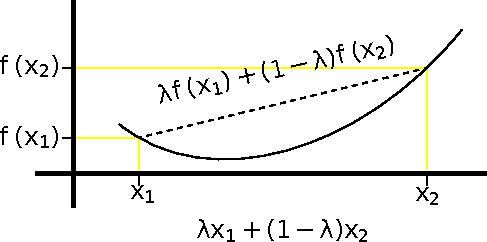
\includegraphics[width=0.5\textwidth]{images/funcao-convexa.pdf}
  %\caption{.}
  \label{fig:funcao-convexa}
  \end{figure}
  \begin{itemize}
  \item $f$ é estritamente convexa se a igualdade for verdadeira 
  apenas para $\lambda = 0$ ou $\lambda = 1$.
  \end{itemize}
\end{frame}

\begin{frame}[allowframebreaks]
  \frametitle{Derivada Segunda e Convexidade}
  \begin{theorem}[derivada segunda e convexidade]
  Se uma função $f$ possui derivada segunda não-negativa (positiva) em um intervalo,
  a função é convexa (estritamente convexa) no intervalo.
  \end{theorem}

  \begin{proof}
  A expansão de Taylor de uma função $f$ em torno do ponto $x_0$ é dada por
  \begin{equation}
  f(x) = f(x_0) + f'(x_0) (x-x_0) + \frac{f''(x^\ast)}{2} (x-x_0)^2
  \end{equation}
  onde $x^\ast \in (x_0,x)$. Por hipótese, $f''(x^\ast) \geq 0$, e desta forma,
  o último termo é não-negativo.

  \proofbreak

  Seja $x_0 = \lambda x_1 + (1-\lambda) x_2$. Analisando em $x=x_1$, teremos
  \begin{eqnarray}
    f(x_1) &\geq& f(x_0) + f'(x_0) (x_1 - \lambda x_1 - (1-\lambda)x_2) \nonumber \\
        &=& f(x_0) + f'(x_0) ((1-\lambda)(x_1-x_2)) \label{eq-274}
  \end{eqnarray}
  Da mesma forma, em $x=x_2$, teremos
  \begin{eqnarray}
    f(x_2) &\geq& f(x_0) + f'(x_0) (x_2 - \lambda x_1 - (1-\lambda)x_2) \nonumber \\
        &=& f(x_0) + f'(x_0) (\lambda(x_2-x_1)) \label{eq-275}
  \end{eqnarray}

  \proofbreak

  Somando $\lambda$ \ref{eq-274} com $(1-\lambda)$ \ref{eq-275}, teremos
  \begin{eqnarray}
  \lambda f(x_1) + (1-\lambda) f(x_2) &\geq& \lambda f(x_0) + \lambda f'(x_0) ((1-\lambda)(x_1-x_2)) + \nonumber \\
                        && (1-\lambda) f(x_0) + (1-\lambda) f'(x_0) (\lambda(x_2-x_1)) \nonumber \\
        &\geq& f(x_0) = f(\lambda x_1 + (1-\lambda) x_2)
  \end{eqnarray}

  \end{proof} 
\end{frame}

\begin{frame}%[allowframebreaks]
  \frametitle{Desigualdade de Jensen}
  \begin{theorem}[Jensen]
  Seja $f$ uma função convexa e $X$ uma variável aleatória, então
  \begin{equation}
    E f(X) = \sum_x p(x) f(x) \geq f(E X) = f \left( \sum_x x p(x) \right)
  \end{equation}
  \end{theorem}

  Se $f$ é estritamente convexa, então $\{E f(X) = f(E(X))\} \Rightarrow \{X = EX\}$,
  o que significa que $X$ é uma v.a. constante.
\end{frame}

\begin{frame}[allowframebreaks]
  \frametitle{Desigualdade de Jensen - demonstração}
  \begin{itemize}
   \item Para uma distribuição de massa com apenas dois pontos.
   \begin{equation}
    E[f(X)] = p_1 f(x_1) + p_2 f(x_2) \geq f(p_1 x_1 + p_2 x_2) = f(EX)
   \end{equation} 
   já que $f$ é convexa e $p_1+p_2=1$.
   \item Para uma distribuição com mais de dois ponto, iremos fazer uma demonstração 
   por indução.
  \end{itemize}

  \begin{proof}
  Suponha que o teorema seja verdadeiro para uma distribuição com $k-1$ pontos de massa.
  Para uma distribuição com $k$ pontos de massa podemos escrever cada 
  $p_i' = p_i / (1-p_k)$ para $i=1,2,\ldots,k-1$. 
  \proofbreak
  Desta forma, teremos
  \begin{eqnarray}
   E[f(X)] &=& \sum_{i=1}^k p_i f(x_i) \nonumber \\
        &=& \sum_{i=1}^{k-1} (1-p_k)p_i' f(x_i) + p_k f(x_k) \nonumber \\
        &=& (1-p_k) \sum_{i=1}^{k-1} p_i' f(x_i) + p_k f(x_k) \nonumber 
   \end{eqnarray}

   \proofbreak

   Poderemos utilizar a hipótese de indução, já que
   \begin{equation}
   \sum_{i=1}^{k-1} p_i' = \sum_{i=1}^{k-1} \frac{p_i}{1-p_k} = \frac{1-p_k}{1-p_k} = 1 .
   \end{equation}
   Então
   \begin{eqnarray}
   E[f(X)] &=& \ldots \nonumber \\
        &\geq& (1-p_k) f\left( \sum_{i=1}^{k-1} p_i' x_i \right) + p_k f(x_k) \nonumber
   \end{eqnarray}
  
   \proofbreak

   Pela definição de convexidade, teremos
   \begin{eqnarray}
   E[f(X)] &=& \ldots \nonumber \\
        &\geq& f \left( (1-p_k) \sum_{i=1}^{k-1} p_i' x_i + p_k x_k \right) \nonumber \\ 
        &=& f\left( \sum_{i=1}^{k} p_i x_i \right)
   \end{eqnarray}

   Desta forma, sendo o teorema válido para uma distribuição de massa com $k-1$ pontos,
   também será verdadeiro para uma distribuição de massa com $k$ pontos.
   Como mostramos que para $k=2$ é verdadeiro, logo o teorema é verdadeiro para qualquer $k$.
  \end{proof}
\end{frame}

\begin{frame}%[allowframebreaks]
  \frametitle{Desigualdade de Jensen - demonstração gráfica}

  \vspace{-0.2cm}
  \begin{figure}[h!]
  \centering
  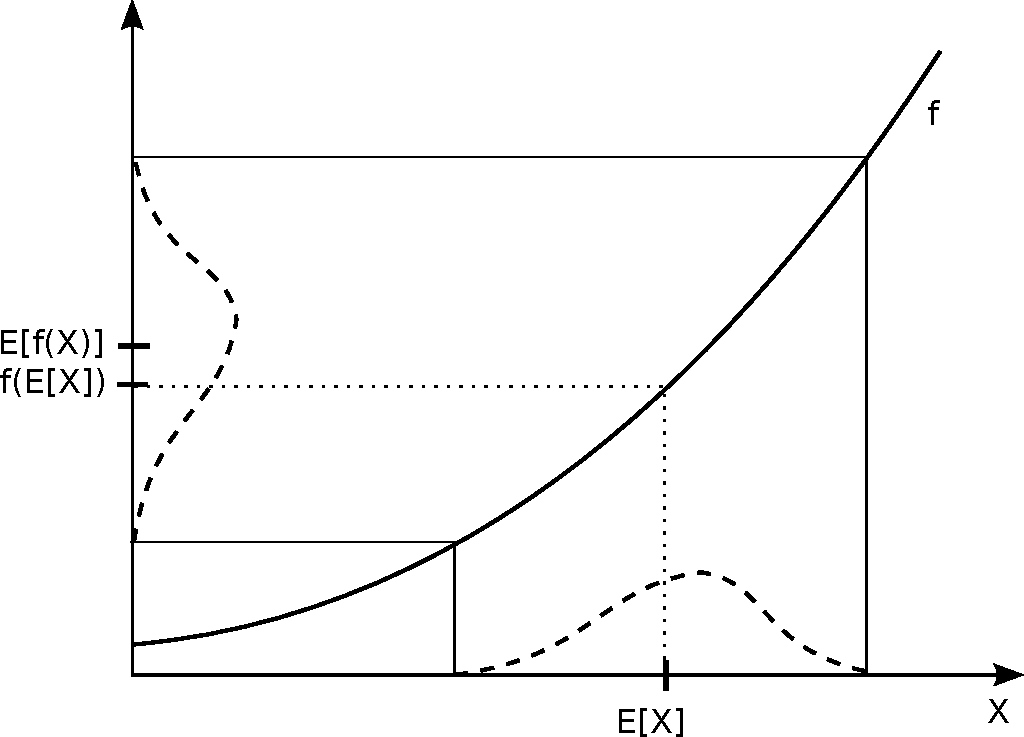
\includegraphics[width=0.5\textwidth]{images/jensen.pdf}
  %\caption{.}
  \label{fig:jensen}
  \end{figure} 

  \vspace{-0.2cm}
  O mapeamento feito pela função convexa $f$ aumenta gradativamente o estiramento
  da distribuição mapeada por $f$ com o aumento dos valores de $X$.
  Desta forma, o valor esperado da distribuição mapeada por $f$ tende a possuir
  um valor maior que o mapeamento por $f$ do valor esperado da distribuição.
\end{frame}


\subsection{Não-Negatividade}
\begin{frame}%[allowframebreaks]
  \frametitle{A divergência de KL é não-negativa}
  \begin{lemma} 
  \begin{equation}
  D(p||q) \geq 0 \text{ com igualdade se e somente se } p(x) = q(x) \forall x.
  \end{equation}
  \end{lemma}
\end{frame}

\begin{frame}%[allowframebreaks]
  \frametitle{A divergência de KL é não-negativa} 
  \begin{proof}
  Mostre que $-D(p||q) \leq 0$. Seja $S_p=\{x: p(x) > 0\} = \sup (p)$, então
  \begin{eqnarray}
  -D(p||q) &=& -\sum_x p(x) \log \frac{p(x)}{q(x)} = -\sum_{x \in S_p} p(x) \log \frac{p(x)}{q(x)} %\nonumber \\
        = \sum_{x \in S_p} p(x) \log \frac{q(x)}{p(x)} = E \log \frac{q(X)}{p(X)} \nonumber \\
        && {\small \text{utilizando a desigualdade de Jensen}} \nonumber \\
        &\leq& \log \left( E \frac{q(X)}{p(X)} \right) = \log \left( \sum_{x \in S_p} p(x) \frac{q(x)}{p(x)} \right) \nonumber \\
        &=& \log \left( \sum_{x \in S_p} q(x) \right) \leq \log \left( \sum_x  q(x) \right) = \log 1 = 0
  \end{eqnarray}
  \end{proof}
\end{frame}

\begin{frame}%[allowframebreaks]
  \frametitle{A divergência de KL é não-negativa}
  \begin{itemize}
  \item Note que $\log x$ é estritamente côncavo.
  \item Então, a igualdade $\sum_{x \in S_p} p(x) \frac{q(x)}{p(x)} = \log \left( \sum_{x \in S_p} p(x) \frac{q(x)}{p(x)} \right)$ significa $Z=E Z$ com $Z = q(X)/p(X)$, então $Z$ é uma variável aleatória constante.
  \item A única constante válida, com $p$ e $q$ sendo distribuições de probabilidade é
  $Z=1$ ou $p(x)=q(x)$.
  \item Então, se $p(x)=q(x)$ teremos $D(p||q)=0$ e vice-versa.
  \end{itemize}
\end{frame}

\begin{frame}%[allowframebreaks]
  \frametitle{A informação mútua é não-negativa}
  \begin{proposition}
  \begin{equation} 
  I(X;Y) \geq 0 \text{ e } I(X;Y) = 0 \Leftrightarrow X \independent Y.
  \end{equation}
  \end{proposition}

  \begin{proof}
  \begin{equation}
  I(X;Y) = D(p(x,y)||p(x)p(y)) \geq 0
  \end{equation}
  \end{proof}
  teremos igualdade se $p(x,y)=p(x)p(y)$, o que é também condição para independência.
\end{frame}

\begin{frame}%[allowframebreaks]
  \frametitle{Informação Mútua}
  \begin{itemize}
  \item $I(X;Y)$ mede o `grau de dependência' entre $X$ e $Y$.
  \item Temos $0 \leq I(X;Y) \leq \min (H(X),H(Y))$.
  \item $I(X;Y) = H(X) - H(X|Y) = H(Y) - H(Y|X)$.
  \item Se $X \independent Y$, então $I(X;Y)=0$, já que em tal caso $H(X|Y)=H(X)$
  e $H(Y|X)=H(Y)$.
  \item Se $X=Y$, então $I(X;Y) = H(X) = H(Y)$ já que em tal caso $H(Y|X)=H(X|Y)=0$.
  \end{itemize}
\end{frame}


\subsection{Limite Superior para a Entropia}
\begin{frame}[allowframebreaks]
  \frametitle{Limite Superior para a Entropia}
  \begin{theorem}
  $H(X) \leq \log \vert \mathcal{X} \vert$, onde $\vert \mathcal{X} \vert$ denota
  o número de elementos da extensão de $X$ (a cardinalidade do domínio), com igualdade
  se e somente se $X$ possuir distribuição uniforme.
  \end{theorem}

  \framebreak

  \begin{proof}
  Seja $u(x) = \frac{1}{\vert \mathcal{X} \vert}$ a função probabilidade de massa uniforme
  em $\mathcal{X}$, e seja $p(x)$ a função probabilidade de massa para $X$. Então
  \begin{eqnarray}
  D(p||u) &=& \sum_{x \in \mathcal{X}} p(x) \log \frac{p(x)}{u(x)} \nonumber \\
        &=& \sum_{x \in \mathcal{X}} p(x) \log p(x) + \sum_{x \in \mathcal{X}} p(x) \log \frac{1}{u(x)} \nonumber \\
        &=& -H(X) + \log \vert \mathcal{X} \vert \sum_{x \in \mathcal{X}} p(x) \nonumber \\
        &=& \log \vert \mathcal{X} \vert - H(X)
  \end{eqnarray}
  \proofbreak
  Como a entropia relativa é não negativa, $D(p||u) \geq 0$, teremos
  \begin{equation}
  D(p||u) = \log \vert \mathcal{X} \vert - H(X) \geq 0
  \end{equation}
  e assim
  \begin{equation}
  H(X) \leq \log \vert \mathcal{X} \vert
  \end{equation}
  \end{proof}
\end{frame}


\subsection{Condicionar Reduz Entropia}
\begin{frame}%[allowframebreaks]
  \frametitle{Condicionar Reduz Entropia}
  Comparando $H(X)$ com $H(X|Y)$, conhecendo $Y$, na média, pode nos dizer algo sobre $X$
  reduzindo a entropia.
  \begin{proposition}
  \begin{equation}
  H(X|Y) \leq H(X) \text{ e } H(X|Y) = H(X) \text{ se e somente se } X \independent Y.
  \end{equation}
  \end{proposition}

  \begin{proof}
  \begin{equation}
  0 \leq I(X;Y) = H(X) - H(X|Y)
  \end{equation}
  \end{proof}

  Poderíamos ter $H(X|Y=y) > H(X)$, mas, na média, $\sum_y p(y) H(X|Y=y) \leq H(X)$.
\end{frame}


\begin{frame}%[allowframebreaks]
  \frametitle{Limite da Entropia para um Conjunto de V.A.}
  A entropia de um conjunto de variáveis aleatórias é maior quando as
  variáveis aleatórias são independentes, há menor redundância entre elas.
  \begin{proposition}\label{prop-lim-ent-conj-va}
  \begin{equation}\label{eq-lim-ent-conj-va}
  H(X_1, X_2, \ldots, X_N) \leq \sum_{i=1}^N H(X_i)
  \end{equation}
  \end{proposition}

  \begin{proof}
  \begin{equation}
  H(X_1, \ldots, X_N) = \sum_{i=1}^N H(X_i | X_1, \ldots, X_{i-1}) \leq \sum_{i=1}^N H(X_i)
  \end{equation}
  \end{proof}

\end{frame}
\note{
 \begin{equation}
 \sum_{i=1}^N H(X_i | X_{\neg i}) = \sum_{i=1}^N H(X_i | X_1, \ldots, X_{i-1}, X_{i+1}, \ldots, X_N) \leq H(X_1, \ldots, X_N)
 \end{equation}
}

\begin{frame}%[allowframebreaks]
  \frametitle{Limites da Independência na Entropia}
  A proposição \ref{prop-lim-ent-conj-va} para duas variáveis é da forma
  \begin{equation}
  H(X_1,X_2) \leq H(X_1) + H(X_2)
  \end{equation}
  Note que a igualdade na Equação \ref{eq-lim-ent-conj-va} é alcançada quando
  todas as variáveis são mutuamente independentes, isto é, quando $X_i \independent X_j \forall i,j$.
\end{frame}


\begin{frame}%[allowframebreaks]
  \frametitle{Condicionamento e Informação Mútua}
  \begin{itemize}
  \item Se $X \independent Y|Z$ então $I(X;Y|Z)=0$. Por exemplo, $X \independent Y|Z$ quando
  $X \rightarrow Z \rightarrow Y$.
  \item Alternativamente, se $Z=Y$, então $I(X;Y|Z)=0$.
  \item Podemos ter $I(X;Y) > I(X;Y|Z)$.
  \item Por outro lado, se $Z=X+Y$ e $X \independent Y$, então $I(X;Y)=0$ mas 
  $I(X;Y|Z)>0$.
  \item Não existe uma relação genérica entre informação mútua e informação mútua condicional.
  \end{itemize}
\end{frame}

\begin{frame}%[allowframebreaks]
  \frametitle{Relações de H}

  \begin{equation}
  H(X) = E I(X) = - \sum_x p(x) \log p(x)
  \end{equation}

  \begin{equation}
  H(X,Y) = - \sum_{x,y} p(x,y) \log p(x,y)
  \end{equation}

  \begin{equation}
  H(Y|X) = - \sum_{x,y} p(x,y) \log p(y|x)
  \end{equation}

  \begin{equation}
  H(X,Y) = H(X) + H(Y|X) = H(Y) + H(X|Y)
  \end{equation}

  \begin{equation}
  I(X;Y) = H(X) - H(X|Y) = H(Y) - H(Y|X)
  \end{equation}

  \begin{equation}
  0 \leq H(X) \leq \log n, \text{ onde } n \text{ é o tamanho do alfabeto de } X.
  \end{equation}
\end{frame}

\begin{frame}%[allowframebreaks]
  \frametitle{Entropia, Informação Mútua, 3 V.A. em um diagrama de Venn}
  \begin{figure}[h!]
  \centering
  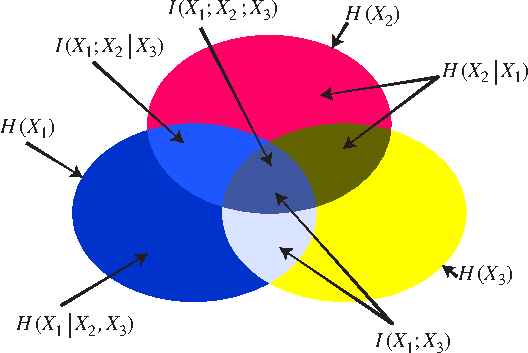
\includegraphics[width=0.7\textwidth]{images/3va-venn.pdf}
  %\caption{.}
  \label{fig:3va-venn}
  \end{figure}
\end{frame}
\note{
\begin{itemize}
 \item $I(X_1;X_2) = I(X_1;X_2|X_3) + I(X_1;X_2;X_3)$.
 \item $I(X_1;X_2) \gtreqqless I(X_1;X_2|X_3)$, mas isto nunca será negativo. 
 \item Então, $I(X_1;X_2;X_3) = I(X_1;X_2) - I(X_1;X_2|X_3)$ pode ser negativo.
 \item $I(X_1;X_2;X_3) = I(X_1;X_2) - I(X_1;X_2|X_3) = I(X_2;X_3) - I(X_2;X_2|X_1) = I(X_3;X_1) - I(X_3;X_1|X_2)$
 \item $I(X_1;X_2;X_3) = H(X_1) + H(X_2) + H(X_3) - H(X_1;X_2) - H(X_2;X_3) - H(X_3;X_1) + H(X_1,X_2,X_3)$
\end{itemize}
}


\begin{frame}[allowframebreaks]
  \frametitle{Revisão}
  \begin{itemize}
  \item divergência de KL: $D(p||q) = \sum_x p(x) \log \frac{p(x)}{q(x)}$
  \item informação mútua: $I(X;Y) = \sum_{x,y} p(x,y) \log \frac{p(x,y)}{p(x)p(y)} = D(p(x,y)||p(x)p(y))$ 
  \item informação mútua condicional: $I(X;Y|Z) = \sum_{x,y,z} p(x,y,z) \log \frac{p(x,y|z)}{p(x|z) p(y|z)} = H(X|Z) - H(X|Y,Z)$
  \item regra da cadeia da informação mútua: $I(X_1,X_2,\ldots,X_N;Y)=\sum_i I(X_i;Y|X_1,X_2,\ldots,X_{i-1})$
  \item entropia relativa condicional: $D(p(y|x)||q(y|x)) \triangleq \sum_{x,y} p(x,y) \log \frac{p(y|x)}{q(y|x)}$
  \item regra da cadeia da divergência de KL: $D(p(x,y)||q(x,y)) = D(p(x)||q(x)) + D(p(y|x)||q(y|x))$
  \item Jensen: $f$ convexa $\Rightarrow$ $E f(X) = \sum_x p(x) f(x) \geq f(E X) = f \left( \sum_x p x(x) \right)$
  \item não negatividade da divergência de KL: $D(p||q) \geq 0$, $D(p||q)=0 \Leftrightarrow p=q$.
  \item não negatividade da informação mútua: $I(X;Y)\geq 0$, $I(X;Y)=0 \Leftrightarrow X \independent Y$.
  \item condicionar reduz a entropia: $H(X) \geq H(X|Y)$, $H(X) = H(X|Y) \Leftrightarrow X \independent Y$.
  \item limite da independência em H: $H(X_1,\ldots,X_N) \leq \sum_{i} H(X_i)$, com igualdade sse todos $X_i$ forem independentes
  \end{itemize}
\end{frame}



\subsection{Medida de Informação}
\begin{frame}%[allowframebreaks]
  \frametitle{Medida de Informação}
  Veremos as correspondências entre a medida de informação de Shannon (e suas manipulações)
  com a teoria de conjuntos. A utilização dos diagramas de informação podem ser utilizadas para 
  simplificar várias demonstrações em teoria da informação.
\end{frame}

\begin{frame}%[allowframebreaks]
  \frametitle{Medida de Informação}
  \begin{itemize}
  \item Temos um conjunto de variáveis aleatórias: $X_1, X_2, \ldots, X_n$.
  \item Para cada variável aleatória associamos um conjunto $\tilde{X}_1, \tilde{X}_2, \ldots, \tilde{X}_n$.
  \end{itemize}

  \begin{definition}[campo (field)]
  Um campo $\mathcal{F}_n$ gerado pelos conjuntos $\tilde{X}_1, \tilde{X}_2, \ldots, \tilde{X}_n$ é
  a coleção de conjuntos que podem ser obtidos através de qualquer sequência de operações
  usuais de conjuntos (união, interseção, complemento, e diferença) sobre os conjuntos 
  $\tilde{X}_1, \tilde{X}_2, \ldots, \tilde{X}_n$.
  \end{definition}

  \begin{definition}[átomo]
  Os átomos de $\mathcal{F}_n$ são os conjuntos da forma $\cap_{i=1}^n Y_i$, onde 
  $Y_i$ é $\tilde{X}_i$ ou $\tilde{X}_i^c$, o complemento de $\tilde{X}_i$.
  \end{definition}
\end{frame}

\begin{frame}%[allowframebreaks]
  \frametitle{Átomos}
  \begin{exampleblock}{átomos - $n=2$}
  Para $n=2$, teremos os conjuntos $\tilde{X}_1, \tilde{X}_2$ e seus complementos,
  respectivamente, $\tilde{X}_1^c, \tilde{X}_2^c$. Existirão $4$ átomos:

  \begin{minipage}[t]{0.35\linewidth}
  \begin{enumerate}
  \item $\tilde{X}_1 \cap \tilde{X}_2$,
  \item $\tilde{X}_1 \cap \tilde{X}_2^c$,
  \item $\tilde{X}_1^c \cap \tilde{X}_2$, e
  \item $\tilde{X}_1^c \cap \tilde{X}_2^c$
  \end{enumerate}
  \end{minipage} \hfill 
  \begin{minipage}[t]{0.55\linewidth}
    \begin{figure}[!ht]
    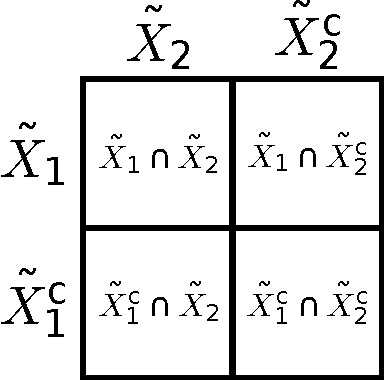
\includegraphics[width=0.5\linewidth]{images/atoms-n2.pdf}
    \end{figure}
  \end{minipage}

  \end{exampleblock}
\end{frame}

\begin{frame}%[allowframebreaks]
  \frametitle{Átomos}
  \begin{exampleblock}{átomos - $n=3$}
  Para $n=3$, teremos os conjuntos $\tilde{X}_1, \tilde{X}_2, \tilde{X}_3$ e seus complementos,  
  respectivamente, $\tilde{X}_1^c, \tilde{X}_2^c, \tilde{X}_3^c$. Existirão $8$ átomos:

  \begin{minipage}[t]{0.35\linewidth}
  \begin{enumerate}
  \item $\tilde{X}_1 \cap \tilde{X}_2 \cap \tilde{X}_3$,
  \item $\tilde{X}_1 \cap \tilde{X}_2 \cap \tilde{X}_3^c$,
  \item $\tilde{X}_1 \cap \tilde{X}_2^c \cap \tilde{X}_3$,
  \item $\tilde{X}_1 \cap \tilde{X}_2^c \cap \tilde{X}_3^c$,
  \item $\tilde{X}_1^c \cap \tilde{X}_2 \cap \tilde{X}_3$, 
  \item $\tilde{X}_1^c \cap \tilde{X}_2 \cap \tilde{X}_3^c$,
  \item $\tilde{X}_1^c \cap \tilde{X}_2^c \cap \tilde{X}_3$, e 
  \item $\tilde{X}_1^c \cap \tilde{X}_2^c \cap \tilde{X}_3^c$
  \end{enumerate}
  \end{minipage} \hfill
  \begin{minipage}[t]{0.6\linewidth}
    \begin{figure}[!ht]
    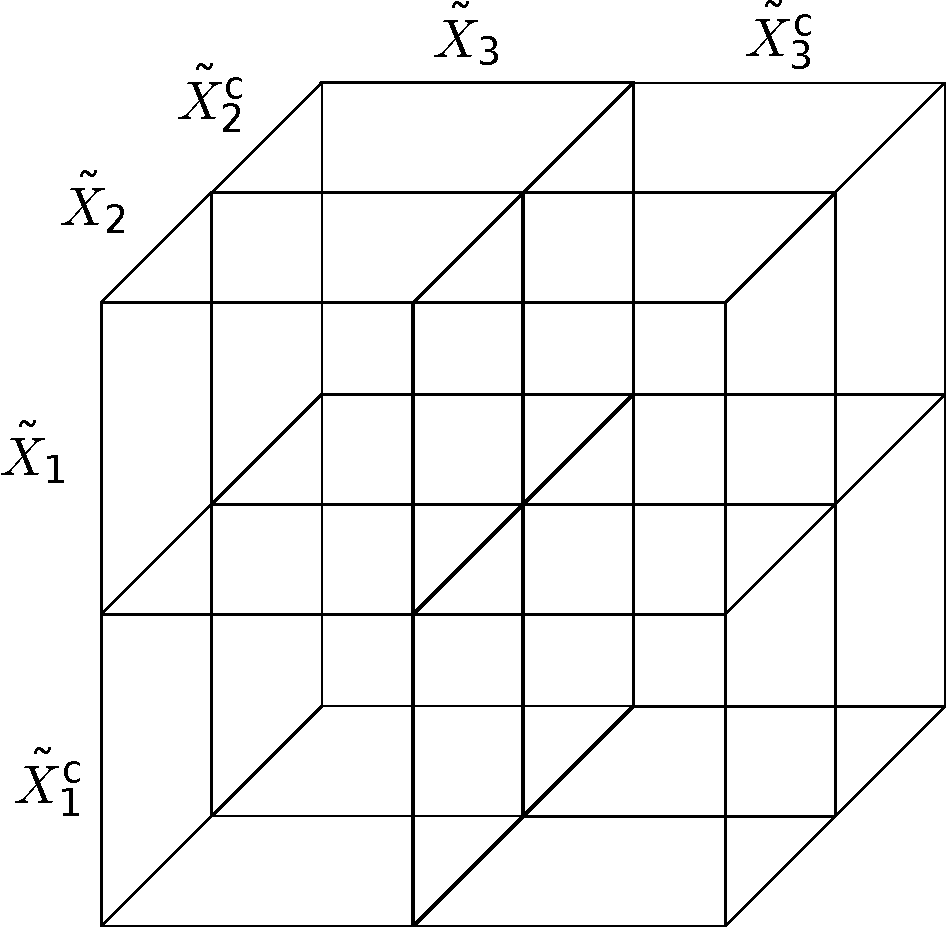
\includegraphics[width=0.6\linewidth]{images/atoms-n3.pdf}
    \end{figure}
  \end{minipage}

  \end{exampleblock}
\end{frame}

\begin{frame}%[allowframebreaks]
  \frametitle{Campo e Átomos}
  \begin{itemize}
  \item existem $2^n$ átomos;
  \item existem $2^{2^n}$ conjuntos no campo $\mathcal{F}_n$;
  \item todos os átomos em $\mathcal{F}_n$ são disjuntos;
  \item todo conjunto em $\mathcal{F}_n$ pode ser expresso de forma única como uma união de um subconjunto dos átomos em $\mathcal{F}_n$.
  \end{itemize}
\end{frame}

\begin{frame}%[allowframebreaks]
  \frametitle{Medida com sinal}
  Em análise matemática, uma medida em um conjunto $S$ é uma forma sistemática de atribuir
  números a todo subconjunto de $S$, sendo intuitivamente interpretada como o seu tamanho.

  Medida com sinal é uma generalização do conceito de medida permitindo que esta assuma valores
  negativos.

  \begin{definition}[medida com sinal]
  Uma função real $\mu$ definida em $\mathcal{F}_n$ é chamada medida com sinal se
  for aditiva no conjunto, i.e., para $A$ e $B$ disjuntos em $\mathcal{F}_n$,
  \begin{equation}
  \mu(A \cup B) = \mu(A) + \mu(B) .
  \end{equation} 
  \end{definition}  
  Para uma medida com sinal $\mu$ teremos $\mu(\emptyset)=0$, já que
  $\mu(A) = \mu(A \cup \emptyset) = \mu(A) + \mu(\emptyset)$.
\end{frame}

\begin{frame}%[allowframebreaks]
  \frametitle{Medida com sinal}
  Uma medida com sinal $\mu$ em $\mathcal{F}_n$ é completamente especificada
  por seus valores nos átomos de $\mathcal{F}_n$. Os valores de $\mu$ em outros
  conjuntos de $\mathcal{F}_n$ podem ser obtidos pela aditividade de conjuntos, 
  já que qualquer $\tilde{X} \in \mathcal{F}_n$ pode ser representado como
  $\tilde{X} = \cup_{i=1} Y_i$, onde $Y_i$ são átomos escolhidos apropriadamente.
\end{frame}


\begin{frame}%[allowframebreaks]
  \frametitle{Medida com sinal}
  \begin{exampleblock}{$n=2$}
  Uma medida com sinal $\mu$ em $\mathcal{F}_2$ é completamente especificada pelos
  valores 
  $\mu( \tilde{X}_1 \cap \tilde{X}_2 )$,
  $\mu( \tilde{X}_1 \cap \tilde{X}_2^c )$,
  $\mu( \tilde{X}_1^c \cap \tilde{X}_2 )$, e
  $\mu( \tilde{X}_1^c \cap \tilde{X}_2^c )$.

  O valor de $\mu$ em $\tilde{X}_1$ pode ser obtido da seguinte forma
  \begin{eqnarray}
  \mu( \tilde{X}_1 ) &=& \mu( (\tilde{X}_1 \cap \tilde{X}_2) \cup ( \tilde{X}_1 \cap \tilde{X}_2^c) ) \nonumber \\
		&=& \mu( \tilde{X}_1 \cap \tilde{X}_2 ) + \mu( \tilde{X}_1 \cap \tilde{X}_2^c ) .
  \end{eqnarray}

  O valor de $\mu$ em $\tilde{X}_1 \setminus \tilde{X}_2$ é dado por
  \begin{equation}
  \mu( \tilde{X}_1 \setminus \tilde{X}_2 ) = \mu( \tilde{X}_1 \cap \tilde{X}_2^c ) .
  \end{equation}

  O valor de $\mu$ em $\tilde{X}_1 \cup \tilde{X}_2$ pode ser obtido através de
  \begin{eqnarray}
  \mu( \tilde{X}_1 \cup \tilde{X}_2 ) &=& \mu( (\tilde{X}_1 \cap \tilde{X}_2) \cup (\tilde{X}_1 \cap \tilde{X}_2^c) \cup (\tilde{X}_1^c \cap \tilde{X}_2) ) \nonumber \\
	&=& \mu( \tilde{X}_1 \cap \tilde{X}_2 ) + \mu( \tilde{X}_1 \cap \tilde{X}_2^c ) + \mu(\tilde{X}_1^c \cap \tilde{X}_2) 
  \end{eqnarray}

  \end{exampleblock}
\end{frame}


\begin{frame}[allowframebreaks]
  \frametitle{Correspondência com a informação de Shannon}
  Os conjuntos $\tilde{X}_1$ e $\tilde{X}_2$ estão associados às variáveis
  aleatória $X_1$ e $X_2$. O campo $\mathcal{F}_2$ é gerado por $\tilde{X}_1$ e $\tilde{X}_2$,
  através dos átomos 
  $(\tilde{X}_1 \cap \tilde{X}_2)$,
  $(\tilde{X}_1 \cap \tilde{X}_2^c)$,
  $(\tilde{X}_1^c \cap \tilde{X}_2)$, e
  $(\tilde{X}_1^c \cap \tilde{X}_2^c)$.
  O diagrama de informação é apresentado na Figura \ref{fig:setX1X2}.

  \begin{figure}[h!]
  \centering
  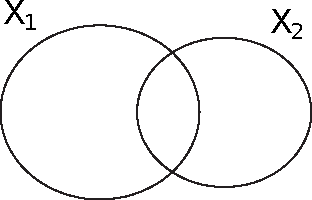
\includegraphics[width=0.4\textwidth]{images/setX1X2.pdf}
  \caption{Diagrama de informação para $X_1$ e $X_2$.}
  \label{fig:setX1X2}
  \end{figure}
 
  O conjunto universo será considerada como sendo $\Omega = \tilde{X}_1 \cup \tilde{X}_2$.
  Desta forma, o átomo $\tilde{X}_1^c \cap \tilde{X}_2^c$ se degenera ao conjunto vazio,
  \begin{equation}
  \tilde{X}_1^c \cap \tilde{X}_2^c = (\tilde{X}_1 \cup \tilde{X}_2)^c = \Omega^c = \emptyset .
  \end{equation}

  Para as v.a.s $X_1$ e $X_2$, as medidas de informação de Shannon são 
  \begin{equation}
  H(X_1), H(X_2), H(X_1|X_2), H(X_2|X_1), H(X_1,X_2), I(X_1;X_2) .
  \end{equation}

  Utilizando a notação $A \cap B^c \equiv A \setminus B$, definimos uma medida com sinal $\mu^\ast$
  \begin{eqnarray}
  \mu^\ast(\tilde{X}_1 \setminus \tilde{X}_2) &=& H(X_1|X_2) ,\\
  \mu^\ast(\tilde{X}_2 \setminus \tilde{X}_1) &=& H(X_2|X_1) ,\\
  \mu^\ast(\tilde{X}_1 \cap \tilde{X}_2) &=& I(X_1;X_2) .
  \end{eqnarray}
  Estes são os valores de $\mu^\ast$ nos átomos não vazios de $\mathcal{F}_2$.
  Os valores de $\mu^\ast$ nos demais conjuntos de $\mathcal{F}_2$ podem ser obtidos por
  adição de conjuntos. Em particular, temos as relações
  \begin{eqnarray}
  \mu^\ast(\tilde{X}_1 \cup \tilde{X}_2) &=& H(X_1, X_2) , \label{eqX1X2HX1X2} \\
  \mu^\ast(\tilde{X}_1) &=& H(X_1) , \label{eqmuX1HX1}\\
  \mu^\ast(\tilde{X}_2) &=& H(X_2) .
  \end{eqnarray}

  Por exemplo, a Equação \ref{eqX1X2HX1X2} pode ser verificada
  \begin{eqnarray}
  \mu^\ast(\tilde{X}_1 \cup \tilde{X}_2) &=& \mu^\ast( (\tilde{X}_1 \setminus \tilde{X}_2) \cup (\tilde{X}_2 \setminus \tilde{X}_1) \cup (\tilde{X}_1 \cap \tilde{X}_2) ) \nonumber \\
	&=& \mu^\ast( \tilde{X}_1 \setminus \tilde{X}_2 ) + \mu^\ast( \tilde{X}_2 \setminus \tilde{X}_1 ) + \mu^\ast( \tilde{X}_1 \cap \tilde{X}_2 ) \nonumber \\
	&=& H(X_1|X_2) + H(X_2|X_1) + I(X_1;X_2) \nonumber \\
	&=& H(X_1, X_2) .
  \end{eqnarray}

  A Equação \ref{eqmuX1HX1} também pode ser facilmente verificada
  \begin{eqnarray}
  \mu^\ast(\tilde{X}_1) &=& \mu^\ast( (\tilde{X}_1 \cap \tilde{X}_2) \cup (\tilde{X}_1 \cap \tilde{X}_2^c) ) \nonumber \\
	&=& \mu^\ast(\tilde{X}_1 \cap \tilde{X}_2) + \mu^\ast(\tilde{X}_1 \cap \tilde{X}_2^c) \nonumber \\
	&=& I(X_1;X_2) + H(X_1|X_2) = H(X_1) .
  \end{eqnarray}

  É possível então verificar a seguinte correspondência com as medidas de informação de Shannon
  \begin{eqnarray}
  H / I &\leftrightarrow& \mu^\ast \\
  , &\leftrightarrow& \cup \\
  ; &\leftrightarrow& \cap \\
  | &\leftrightarrow& \setminus 
  \end{eqnarray}

  \begin{itemize}
  \item obs.: com a notação de medida, não existe distinção entre $H$ e $I$, podemos escrever
	$H(X;Y) = I(X;Y)$, utilizando a notação do ponto-e-vírgula.
  \end{itemize}
\end{frame}



\subsection{Desigualdade da soma de logaritmos}
\begin{frame}%[allowframebreaks]
  \frametitle{Desigualdade da soma de logaritmos}
  \begin{theorem}[desigualdade da soma de logaritmos]
  Dados $(a_1, \ldots, a_n)$ e $(b_1,\ldots,b_n)$, com $a_i \geq 0$ e $b_i \geq 0$, temos
        \begin{equation}
         \sum_{i=1}^n a_i \log \frac{a_i}{b_i} \geq \left( \sum_{i=1}^n a_i \right) \log \frac{\sum_{i=1}^n a_i}{\sum_{i=1}^n b_i}
        \end{equation}
  e teremos igualdade sse $a_i/b_i = c = \text{const.}$.
  \end{theorem}

  \begin{itemize}
  \item Relembrando: $0 \log 0 = 0$, $a \log a/0 = \infty$ para $a>0$, e $0 \log 0/0 =0$.
  \item A desigualdade da soma de logaritmos é utilizada para demonstrar algumas propriedades importantes.
  \end{itemize}
\end{frame}

\begin{frame}%[allowframebreaks]
  \frametitle{Desigualdade da soma de logaritmos}

  Considere $f(t) = t \log t = t (\ln t) (\log e)$, que é estritamente convexa, pois
  $f''(t) = 1/t \log e >0$, $\forall t > 0$.
  
  \begin{figure}[h!]
  \centering
  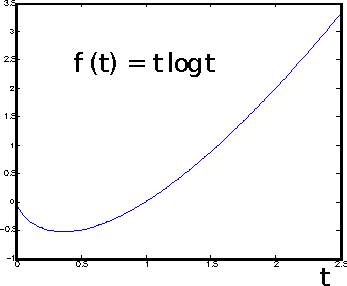
\includegraphics[width=0.4\textwidth]{images/tlogt.pdf}
  %\caption{.}
  \label{fig:tlogt}
  \end{figure}
\end{frame}

\begin{frame}[allowframebreaks]
  \frametitle{Desigualdade da soma de logaritmos}
  \begin{proof}
        \begin{itemize}
        \item Dada $f$ convexa, a desigualdade de Jensen diz que
          \begin{equation}
          \sum_i \alpha_i f(t_i) \geq f \left( \sum_i \alpha_i t_i \right) \text{ com } \alpha_i \geq 0 \text{ e } \sum_i \alpha_i = 1
          \end{equation}

        \item $f(x) = x \log x$ é estritamente convexa para $x>0$, já que 
                $f''(x)=\frac{1}{x} \log e > 0$ para $x>0$.

        \end{itemize}
        \proofbreak
        \begin{itemize}
        \item Vamos fazer $\alpha_i = \nicefrac{b_i}{\sum_{j=1}^n b_j}$ e $t_i = \nicefrac{a_i}{b_i}$, então teremos
        \begin{eqnarray}
        \sum_i \alpha_i f(t_i) &\geq& f \left( \sum_i \alpha_i t_i \right) \nonumber \\
        \sum_i \left( \frac{b_i}{\sum_j b_j} f \left( \frac{a_i}{b_i} \right) \right) &\geq&
                f \left( \sum_i \frac{b_i}{\sum_j b_j} \frac{a_i}{b_i} \right) \nonumber
        \end{eqnarray}
        \end{itemize}

   \proofbreak
   \vspace{-2ex}
   \begin{eqnarray}
        \sum_i \left( \frac{b_i}{\sum_j b_j} f \left( \frac{a_i}{b_i} \right) \right) &\geq&
                f \left( \sum_i \frac{b_i}{\sum_j b_j} \frac{a_i}{b_i} \right) \nonumber \\
        \frac{1}{\sum_j b_j} \sum_i \left( b_i \frac{a_i}{b_i} \log \frac{a_i}{b_i} \right) &\geq&
                \left( \sum_i \frac{a_i}{\sum_j b_j} \right) \log \sum_i \frac{a_i}{\sum_j b_j} \nonumber \\
        \sum_i a_i \log \frac{a_i}{b_i} &\geq& \left( \sum_i a_i \right) \log \sum_i \frac{a_i}{\sum_j b_j} \nonumber \\
        \sum_i a_i \log \frac{a_i}{b_i} &\geq& \sum_i a_i \log \frac{\sum_i a_i}{\sum_j b_j}
   \end{eqnarray}

  \end{proof}
\end{frame}


\subsection{Divergência é não negativa}
\begin{frame}%[allowframebreaks]
  \frametitle{Divergência é não negativa}
  A desigualdade da soma de logaritmos pode ser utilizada para mostrar que $D(p||q) \geq 0$.
  \begin{proof}
        \begin{eqnarray}
        D(p||q) &=& \sum_x p(x) \log \frac{p(x)}{q(x)} \nonumber \\
                &\geq& \left( \sum_x p(x) \right) \log \frac{\sum_x p(x)}{\sum_x q(x)} \nonumber \\
                &=& 1 \log \frac{1}{1} = 0
        \end{eqnarray}
  \end{proof}
\end{frame}

\subsection{Entropia Relativa é Convexa no Par}
\begin{frame}[allowframebreaks]
  \frametitle{A Entropia Relativa é Convexa no Par}
  \begin{theorem}
  Seja $(p_1, q_1)$ e $(p_2, q_2)$ dois pares de função massa probabilidade, então
    \begin{equation}
        D(\lambda p_1 + (1 - \lambda) p_2 || \lambda q_1 + (1- \lambda)q_2) \leq \lambda D(p_1 || q_1) + (1- \lambda) D(p_2 || q_2) ,
    \end{equation}
    para todo $0 \leq \lambda \leq 1$.
  \end{theorem}

  \framebreak

  \begin{proof}
  Pela definição da divergência de KL, temos
    \begin{multline}
    D(\lambda p_1 + (1 - \lambda) p_2 || \lambda q_1 + (1- \lambda)q_2) = \\
        \sum_x (\lambda p_1(x) + (1 - \lambda) p_2(x) ) \log \frac{\lambda p_1(x) + (1 - \lambda) p_2(x)}{\lambda q_1(x) + (1 - \lambda) q_2(x)}
    \end{multline}
    cada termo do somatório é da forma
    \begin{equation}
        ( \lambda p_1(x) + (1 - \lambda) p_2(x) ) \log \frac{\lambda p_1(x) + (1 - \lambda) p_2(x)}{\lambda q_1(x) + (1 - \lambda) q_2(x)} = \left( \sum_i a_i \right) \log \frac{\sum_i a_i}{\sum_i b_i}
    \end{equation}

  \proofbreak

  Utilizando a desigualdade da soma dos logaritmos 
  \begin{eqnarray}
  \left( \sum_i a_i \right) \log \frac{\sum_i a_i}{\sum_i b_i} &\leq&
        \sum_i a_i \log \frac{a_i}{b_i} \nonumber \\
        &=& a_1 \log \frac{a_1}{b_1} + a_2 \log \frac{a_2}{b_2} \nonumber \\
        &=& \lambda p_1(x) \log \frac{\lambda p_1(x)}{\lambda q_1(x)} + (1 - \lambda) p_2(x) \log \frac{(1 - \lambda) p_2(x)}{(1-\lambda) q_2(x)} \nonumber \\
        &=& \lambda D(p_1 || q_1) + (1 - \lambda) D(p_2 || q_2)
  \end{eqnarray}
  \end{proof}
\end{frame}
\note{
        \begin{itemize}
        \item Note que podemos fazer $q_1 = q_2$ e desta forma obteremos convexidade apenas em $p$.
        \item Este é o fundamento para o procedimento de minimização alternada, que
        é um caso especial do algoritmo de EM (maximização da esperança), 
        para o cálculo da função de taxa de distorção,
        e para o cálculo da função geral de capacidade de canal.
        \end{itemize}
}

\subsection{Concavidade da Entropia}
\begin{frame}[allowframebreaks]
  \frametitle{A Entropia é Concava}
  \begin{theorem}
  $H(p)$ é uma função concava de $p$.
  \end{theorem}

  \framebreak
  \begin{proof}
  \vspace{-4ex}
  \begin{eqnarray}
    H(p) &=& - \sum_i p_i \log p_i = - \sum_i p_i \log p_i  + \log \vert \mathcal{X} \vert - \log \vert \mathcal{X} \vert \nonumber \\
        &=& \log \vert \mathcal{X} \vert - \sum_i p_i \log p_i - \log \vert \mathcal{X} \vert \underbrace{\sum_i p_i}_{=1} \nonumber \\
        &=& \log \vert \mathcal{X} \vert - \sum_i \left( p_i \log p_i + p_i \log \vert \mathcal{X} \vert \right) \nonumber \\
        &=& \log \vert \mathcal{X} \vert - \sum_i p_i \left( \log p_i -  \log \nicefrac{1}{\vert \mathcal{X} \vert } \right) \nonumber \\
        &=& \underbrace{\log \vert \mathcal{X} \vert}_{\text{constante}} - \underbrace{D(p||u)}_{\text{convexo}}
  \end{eqnarray}
  onde $u$ é a distribuição uniforme.
  \end{proof}
\end{frame}
\note{
Podemos ver a entropia como a similaridade com a distribuição uniforme.
Quanto maior a entropia, mais próximo estaremos da distribuição uniforme.
}

\begin{frame}[allowframebreaks]
  \frametitle{Consequências para a Informação Mútua}
  Seja $(X,Y) \sim p(x,y) = p(x)p(y|x)$, a informação mútua $I(X;Y)$ é uma função côncava
  de $p(x)$ para $p(y|x)$ fixo e uma função convexa de $p(y|x)$ para $p(x)$ fixo.

  \framebreak
  \begin{proof}
    \begin{itemize} \item $I(X;Y)$ é uma função côncava de $p(x)$ para $p(y|x)$ fixo \end{itemize}
    \vspace{-2ex}
    \begin{eqnarray}
    I(X;Y) &=& D(p(x,y)||p(x)p(y)) \text{ (definição) } \nonumber \\
        &=& \sum_{x,y} p(x,y) \log \frac{p(x,y)}{p(x)p(y)} \text{ (definição) } \nonumber \\
        &=& \sum_{x,y} p(x)p(y|x) \log \frac{ p(x)p(y|x) }{p(x) \sum_x p(x) p(y|x)}
    \end{eqnarray}
    Se $p(y|x)$ é constante, então a informação mútua é função de $p(x)$
    \vspace{-1ex}
    \begin{equation}
    I_{p(x)} (X;Y) = \sum_{x,y} p(x) p(y|x) \log \frac{p(x) p(y|x)}{p(x) \sum_x p(x) p(y|x)}
    \end{equation}  

    \proofbreak
    
    \begin{equation}
    I_{p(x)} (X;Y) = \sum_{x,y} p(x) p(y|x) \log \frac{p(x) p(y|x)}{p(x) \sum_x p(x) p(y|x)}
    \end{equation}

    Utilizando a propriedade da convexidade da divergência de Kullback-Leibler
    \begin{equation}\label{eq-Imixpx}
    I_{\lambda p_1(x) + (1-\lambda)p_2(x)} (X;Y) \geq \lambda I_{p_1(x)} (X;Y) + (1-\lambda) I_{p_2(x)} (X;Y)
    \end{equation}
    então a informação mútua é uma função concava de $p(x)$ para $p(y|x)$ fixo.


    \proofbreak

    \begin{itemize} \item $I(X;Y)$ é uma função convexa de $p(y|x)$ para $p(x)$ fixo \end{itemize}
    Aplicamos a mesma ideia, porém agora consideraremos $p(x)$ fixo.
    \begin{equation}
    I_{p(y|x)} (X;Y) = \sum_{x,y} p(x) p(y|x) \log \frac{p(x) p(y|x)}{p(x) \sum_x p(x) p(y|x)}
    \end{equation}

    Utilizando a propriedade da convexidade da divergência de Kullback-Leibler
    \begin{equation}\label{eq-Imixpxy}
    I_{\lambda p_1(y|x) + (1-\lambda)p_2(y|x)} (X;Y) \leq \lambda I_{p_1(y|x)} (X;Y) + (1-\lambda) I_{p_2(y|x)} (X;Y)
    \end{equation}

  \end{proof}
\end{frame}
\note{
Estes resultados serão importantes para a capacidade de canal e vários outras
otimizações envolvendo informação mútua e distribuições.
}

\begin{frame}[allowframebreaks]
  \frametitle{Informação Mútua, Comunicação e Convexidade}

  Envio de informação por um canal ruidoso.
  \begin{figure}[h!]
  \centering
  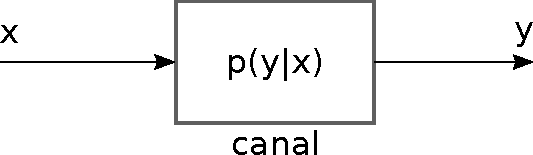
\includegraphics[width=0.5\textwidth]{images/canal_pyx.pdf}
  %\caption{.}
  \label{fig:3va-venn}
  \end{figure}

  \begin{itemize}
        \item Canal: processo ruidoso, para cada $x$ temos uma distribuição sobre os possíveis $y$ recebidos
        \item A taxa de informação transmitida de $X$ para $Y$, por utilização do canal,
        em unidades de bits, é $I(X;Y)$.
  \end{itemize}
\end{frame}
\note{
  \begin{itemize}
        \item Embaralhando $p(x)$ não pode diminuir (pode aumentar ou não alterar) 
        a transmissão de informação para um canal fixo, com relação à original mistura de taxas
        (ver Equação \ref{eq-Imixpx}).
        \item Embaralhando $p(y|x)$ para um canal ruidoso e uma fonte fixa, podemos apenas
        não aumentar (pode reduzir ou manter constante) a taxa de transmissão, em relação
        à original mistura de taxas (ver Equação \ref{eq-Imixpxy}).
  \end{itemize}
}



\section{Processamento de Dados}
\subsection{Desigualdade do Processamento de Dados}

\begin{frame}%[allowframebreaks]
  \frametitle{Desigualdade do Processamento de Dados}
  Dada uma fonte de informação, é possível utilizar alguma forma de processamento de dados
  de forma a obter mais informação sobre esta fonte?

  \begin{figure}[h!]
  \centering
  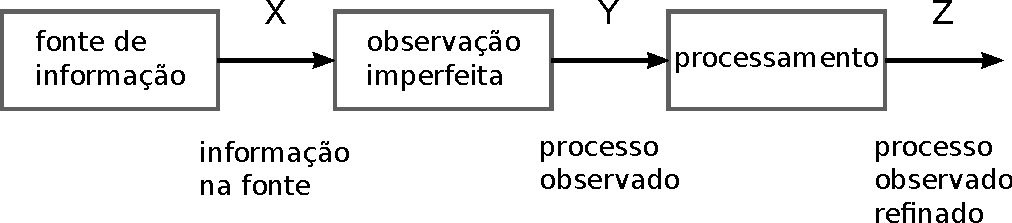
\includegraphics[width=0.8\textwidth]{images/proc-data.pdf}
  %\caption{.}
  \label{fig:proc-data}
  \end{figure} 
\end{frame}

\begin{frame}%[allowframebreaks]
  \frametitle{Desigualdade do Processamento de Dados}
  \begin{itemize}
  \item Imagens com ISO elevado são ruidosas, mas são a única forma de obtermos uma foto
        em baixa luminosidade com pequena abertura (ampla profundidade de campo).
  \item O objetivo da remoção de ruído é recuperar a imagem original.
  \end{itemize}

  \begin{figure}[h!]
  \centering
  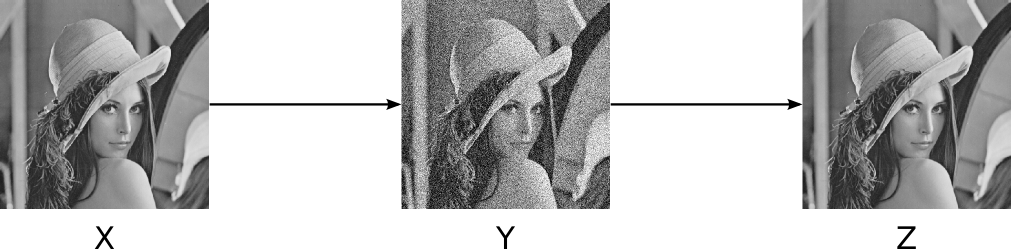
\includegraphics[width=0.8\textwidth]{images/lena-denoising.png}
  %\caption{.}
  \label{fig:lena-denoising}
  \end{figure}

  \begin{itemize}
  \item É possível obter mais informação sobre uma fonte através de processamento adicional?
  \pause
  Infelizmente não.
  \end{itemize}
\end{frame}
\note{
Profundidade de campo descreve até que ponto objetos que estão mais ou menos perto do plano de foco aparentam estar nítidos. 

Regra geral, quanto menor for a abertura do diafragma/íris (maior o valor f/x), para uma mesma distância do objecto fotografado, maior será a distância do plano de foco a que os objetos podem estar enquanto permanecem nítidos.
}

\subsection{Cadeia de Markov}
\begin{frame}[allowframebreaks]
  \frametitle{Cadeia de Markov}
  \begin{definition}[Cadeia de Markov]
  As variáveis aleatórias $X$, $Y$ e $Z$ formam uma cadeia de Markov nesta ordem
  (denotado $X \rightarrow Y \rightarrow Z$) se a distribuição condicional de $Z$
  depende apenas de $Y$ e é condicionalmente independente de $X$. Especificamente,
  $X$, $Y$ e $Z$ formam uma cadeia de Markov $X \rightarrow Y \rightarrow Z$ se
  a função massa de probabilidade conjunta pode ser escrita como
  \begin{equation}
  p(x,y,z) = p(x) p(y|x) p(z|y)
  \end{equation}
  \end{definition}

  \begin{itemize}
  \item $X \rightarrow Y \rightarrow Z$ sse $X$ e $Z$ são condicionalmente independentes
  dado $Y$ ($X \independent Z | Y$). Isto é,
  \begin{equation}
  p(x,z|y) = \frac{p(x,y,z)}{p(y)} = \frac{p(x)p(y|x)p(z|y)}{p(y)} = p(x|y) p(z|y) \ \ \forall x,y,z
  \end{equation}
  \end{itemize}

  \framebreak

  \begin{itemize}
  \item $X \rightarrow Y \rightarrow Z$ implica em $Z \rightarrow Y \rightarrow X$
  \end{itemize}
  \begin{proof}
  \begin{eqnarray}
        p(x,y,z) &=& p(x)p(y|x)p(z|y) = p(x,y)p(z|y) \nonumber \\
                &=& \frac{p(x,y)p(z|y)p(y)}{p(y)} = p(x|y) p(y,z) \nonumber \\
                &=& p(x|y) p(y|z) p(z)
  \end{eqnarray}
  \end{proof}

  \begin{figure}[h!]
  \centering
  
\includegraphics[width=0.8\textwidth]{images/chainxyz.pdf}
  %\caption{.}
  \label{fig:chain}
  \end{figure}

  \begin{itemize}
  \item Se $Z=f(Y)$, então $X \rightarrow Y \rightarrow Z$ (i.e., $X$, $Y$ e $Z$ formam
        uma cadeia de Markov). $f(\cdot)$ pode ser aleatória ou determinística. 
        $X$ é irrelevante para determinar $Z$ quando $Y$ é dado.
  \end{itemize}
\end{frame}

\begin{frame}[allowframebreaks]
  \frametitle{Desigualdade do Processamento de Dados}
  \begin{theorem}[Desigualdade do Processamento de Dados]
   Se $X \rightarrow Y \rightarrow Z$ então
  \begin{equation}
        I(X;Y) \geq I(X;Z)
  \end{equation}
  \end{theorem}
  \begin{itemize}
  \item Na cadeia de Markov, as setas correspondem ao processamento e as variáveis aleatórias 
        correspondem aos dados.
  \item O processamento pode ser aleatório ou determinístico.
  \item A desigualdade de processamento de dados diz que ao efetuar mais processamento dos dados,
        só é possível perder informação sobre a fonte original, quando medida pela informação mútua.
  \end{itemize}

  \framebreak

  \begin{proof}
  Utilizando a regra da cadeia da informação mútua, teremos
  \begin{eqnarray}
  I(X;Y,Z) &=& I(X;Z) + I(X;Y|Z) \nonumber \\
        &=& I(X;Y) + I(X;Z|Y)
  \end{eqnarray}
  Como $X \independent Z |Y$ ($X$ e $Z$ são condicionalmente independentes, dado $Y$), temos
  que $I(X;Z|Y)=0$. Como $I(X;Y|Z) \geq 0$, teremos
  \begin{equation}
  I(X;Z) + \underbrace{I(X; Y|Z)}_{\geq 0} = I(X;Y) + \bcancelto{0}{I(X;Z|Y)}
  \end{equation}
  Então
  \begin{equation}
  I(X;Z) \leq I(X;Y)
  \end{equation}
  \end{proof}

  \begin{itemize}
  \item Teremos igualdade sse $I(X;Y|Z)=0$ (i.e. $X \rightarrow Z \rightarrow Y$).
  \item De forma similar, podemos mostrar que $I(Y;Z) \geq I(X;Z)$.
  \end{itemize}

  \begin{corollary}
   Se $Z=g(Y)$, então $I(X;Y) \geq I(X;g(Y))$.

  Demonstração: $X \rightarrow Y \rightarrow g(Y)$ forma uma cadeia de Markov.
  \end{corollary}

  \begin{corollary}
  Se $X \rightarrow Y \rightarrow Z$ então $I(X;Y|Z) \leq I(X;Y)$.

  \begin{equation}
  \underbrace{I(X;Z)}_{\geq 0} + I(X; Y|Z) = I(X;Y) + \bcancelto{0}{I(X;Z|Y)}
  \end{equation}
  então
  \begin{equation}
  I(X; Y|Z) \leq I(X;Y)
  \end{equation}
  \end{corollary}

  \begin{itemize}
  \item Processamento pode apenas perder informação sobre $X$.
        Quando $X$ é a fonte e $Y$ o receptor, nenhum processamento irá aumentar a informação sobre $X$.
  \item Considere o reconhecimento de padrões: $X$ é um objeto, $Y$ é uma lista de características
        e $f(Y)$ é processamento subsequente. Então, qualquer processamento subsequente poderá apenas
        reduzir a informação sobre o objeto.
  \item Como funciona então as técnicas de remoção de ruído em imagens ou áudio?
        \begin{itemize}
        \item  As técnicas supõem o conhecimento de algumas informações sobre a imagem original, ou seja,
          utilizam conhecimento \textit{a priori} para processar a imagem. 
        \end{itemize}
  \end{itemize}
  
  \begin{corollary}
  Se $X \rightarrow Y \rightarrow Z$, então $I(X; Y|Z) \leq I(X;Y)$. I.e.,
  $I(X; Y|Z) = H(X|Z) - H(X|Y,Z) \leq H(X) - H(X|Y)$.
  \end{corollary}
  
\end{frame}




\subsection{Estatística Suficiente}
\begin{frame}[allowframebreaks]
  \frametitle{Estatística T}

  \begin{example}
  Seja $X_1, X_2, \ldots, X_N$, $X_i \in \{0,1\}$ uma sequência i.i.d. de arremessos de moeda,
  $p(X=1)=\theta = 1 - P(X=0)$.

  Faça $T(X_1,\ldots,X_N) = \sum_{i=1}^{^N} X_i$, contagem do número de \textit{caras}.

  Dizemos que $T$ é uma \textbf{estatística} da amostra.
  \end{example}
  
  \begin{itemize}
  \item De forma geral, uma estatística é uma função de uma coleção de variáveis aleatórias
        (e.g., uma média empírica, uma variância empírica, ou um máximo empírico, etc)
  \item Uma estatística é por sua vez uma v.a.
  \item Uma boa estatística possui informação útil sobre as amostras, enquanto uma 
        estatística ruim não (por exemplo $T(X_1, \ldots, X_N)=X_1)$.
  \item As estatísticas costumam ser chamadas de `características' no contexto de reconhecimento
        de padrões e aprendizado de máquina.
  \end{itemize}
\end{frame}

\begin{frame}[allowframebreaks]
  \frametitle{Ensaio de Bernoulli}
  \begin{itemize}
  \item Considere a estatística de contagem citada anteriormente. 
  \item Uma vez que sabemos a estatística, a probabilidade de uma sequência pode ser expressa
        sem fazer referência à $\theta$ (parâmetro que caracteriza a distribuição).
        \begin{multline}
        p(x_1,\ldots,x_N|T(x_1,\ldots,x_N),\theta) = p(x_1,\ldots,x_N|T(x_1,\ldots,x_N)) \\
        = \begin{cases} 
                \frac{1}{{N \choose k}} &  \sum_i x_i = k \\
                0       & \text{caso contrário}
        \end{cases}
        \end{multline}
  \item Em outras palavras: $X_{1:N} \independent \theta | T(X_{1:N})$.
  \item Isto implica na cadeia de Markov: $\theta \rightarrow T(X_{1:N}) \rightarrow X_{1:N}$
  \item Por outro lado, sabemos que $T(X_{1:N})$ é uma função de $X_{1:N}$.
  \item Desta forma, também temos a seguinte cadeia de Markov: $\theta \rightarrow X_{1:N} \rightarrow T(X_{1:N})$
  \end{itemize}
\end{frame}

\begin{frame}[allowframebreaks]
  \frametitle{Desigualdade de Processamento de Dados e Estatística}
  \begin{itemize}
  \item cadeia de Markov (A): $\theta \rightarrow T(X_{1:N}) \rightarrow X_{1:N}$.
  \item pela desigualdade de processamento de dados em (A) teremos: $I(\theta;T(X_{1:N})) \geq I(\theta;X_{1:N})$.
  \item cadeia de Markov (B): $\theta \rightarrow X_{1:N} \rightarrow T(X_{1:N})$.
  \item pela desigualdade de processamento de dados em (B) teremos: $I(\theta;X_{1:N}) \geq I(\theta;T(X_{1:N}))$.
  \item então, (A) e (B) $\Rightarrow$ $I(\theta;X_{1:N}) = I(\theta;T(X_{1:N}))$, e nenhuma 
        informação é perdida sobre $\theta$ indo de $X_{1:N}$ para $T(X_{1:N})$.
  \end{itemize}
  
  \begin{definition}[Estatística Suficiente]
  Uma função $T(\cdot)$ é dita ser uma estatística suficiente em relação à família
  $\{f_{\theta} (x)\}$ se $X$ é independente de $\theta$ dado $T(X)$ para qualquer
  distribuição em $\theta$ (i.e. $\theta \rightarrow T(X) \rightarrow X$ forma uma
  cadeia de Markov). Então 
  \begin{equation}
  I(\theta ; X) = I(\theta ; T(X)) \ \forall \theta
  \end{equation}
  Uma estatística suficiente preserva a informação mútua e reciprocamente
  \begin{equation}
  X \independent \theta | T(X)
  \end{equation}
  \end{definition}
  \begin{itemize}
  \item i.e., uma cadeira de Markov (A) é condição suficiente para suficiência de uma estatística.
  \item uma estatística suficiente é utilizada para estimar os parâmetros a partir dos dados:
  no limite em que temos infinitos dados, teremos uma estimativa exata (consistência assintótica).
  \end{itemize}
\end{frame}


\begin{frame}[allowframebreaks]
  \frametitle{Estatística Suficiente}
  \begin{example}
  Seja $X_1, \ldots, X_N$, $X_i \in \{0,1\}$, uma sequência i.i.d. de lances de uma moeda 
  com parâmetro $\theta = Pr(X_i=1)$. Dado $N$, o número de 1's é uma estatística suficiente
  para $\theta$.
  \begin{equation}
  T(X_1, \ldots, X_N) = \sum_{i=1}^{N} X_i
  \end{equation}
  Dado $T$, todas as sequências com o mesmo número de 1's são igualmente prováveis e independentes
  do parâmetro $\theta$.

  \examplebreak

  Existem ${N \choose k}$ sequências de comprimento $N$ com $k$ 1's e são todas equiprováveis.
  $Pr(X_{1:N} = x_{1:N}) = \theta^k (1-\theta)^{N-k}$. Então
  \begin{equation}
  Pr\{(X_1,\ldots,X_N)=(x_1,\ldots,x_N) | \sum_{i=1}^N X_i = k\} = 
        \begin{cases} 
                \frac{1}{{N \choose k}} &  \text{ se } \sum_i x_i = k \\
                0       & \text{caso contrário}
        \end{cases}
  \end{equation}
  Temos então que $\theta \rightarrow \sum X_i \rightarrow (X_1,\ldots,X_N)$ forma uma cadeia de Markov
  e $T$ é uma estatística suficiente para $\theta$ (dado $\sum X_i$, a sequência $(X_1,\ldots,X_N)$ é
  estatisticamente independente de $\theta$).
  \end{example}
\end{frame}


\begin{frame}[allowframebreaks]
  \frametitle{Teorema da Fatoração de Fisher-Neyman}
  \begin{theorem}[Teorema da Fatoração de Fisher-Neyman]
  Se a função densidade de probabilidade é $f_\theta (x)$, então $T$ é suficiente para $\theta$
  se e somente se podemos encontrar funções não-negativas $g$ e $h$ tais que
  \begin{equation}
  f_\theta (x) = h(x) g_\theta (T(x)) ,
  \end{equation}
  i.e., a densidade $f$ pode ser fatorada em um produto tal que um fator $h$ não depende de $\theta$
  e o outro fator, que depende de $\theta$, dependerá de $x$ apenas por meios de $T(X)$.
  \end{theorem}
\end{frame}

\begin{frame}[allowframebreaks]
  \frametitle{Estatística Suficiente}
        \begin{theorem}[Estatística Suficiente]
        $T(\cdot)$ é suficiente para $\theta$ sse a probabilidade $p(x_{1:N}|\theta)$
        pode ser escrita como o produto
        \begin{equation}
        p(x_{1:N}|\theta) = g(T,\Theta)h(x_{1:N})
        \end{equation}
        \end{theorem}

        \begin{eqnarray}
        p(x_{1:N}|\theta) &=& g(T,\Theta)h(x_{1:N}) \nonumber \\
                        &=& g(T,\Theta)h(x_{1:N}, T(x_{1:N}))
        \end{eqnarray}

        \framebreak

        \begin{definition}[Independencia Condicional]
        Dadas três variáveis aleatórias $A,B,C$, temos que $A\independent B \vert C$ sse
        existem funções $g$ e $h$ tais que $p(a,b,c)$ possa ser reescrita na forma
                \begin{equation}
                p(a,b,c) = g(a,c) h(b,c)
                \end{equation}
        \end{definition}
\end{frame}

\begin{frame}[allowframebreaks]
  \frametitle{Estatística Suficiente}
  \begin{example}
        Se $X$ possui distribuição normal com média $\theta$ e variância $1$
        \begin{equation}
        f_\theta (x) = \frac{1}{\sqrt{2\pi}} e^{-(x-\theta)^2/2} = N(\theta,1)
        \end{equation}
        e $X_1,\ldots,X_n$ são tiradas de forma independente de acordo com esta distribuição.
        Uma estatística suficiente para $\theta$ é a média amostral
        \begin{equation}
        \overline{X_n} = \frac{1}{n} \sum_{i=1}^{n} X_i
        \end{equation}

        \examplebreak
	\vspace{-6ex}
        \begin{eqnarray}
        f_\theta (x_1,\ldots,x_n) &=& \left( \frac{1}{\sqrt{2\pi}} \right)^n e^{-\frac{1}{2} \sum_{i=1}^n (x_i - \theta)^2} \nonumber \\
                &=& \left( \frac{1}{\sqrt{2\pi}} \right)^n e^{-\frac{1}{2} \sum_{i=1}^n x_i^2} e^{\sum_{i=1}^n (x_i \theta - \theta^2/2)} \nonumber \\
                &=& \left( \frac{1}{\sqrt{2\pi}} \right)^n e^{-\frac{1}{2} \sum_{i=1}^n x_i^2} e^{\theta n \left( \frac{1}{n} \sum_{i=1}^n x_i - \frac{\theta}{2} \right)} \nonumber \\
                &=& \underbrace{ \left( \frac{1}{\sqrt{2\pi}} \right)^n e^{-\frac{1}{2} \sum_{i=1}^n x_i^2} }_{h(x_1,\ldots,x_n)} \underbrace{ e^{\theta n \left( T(X_{1:n}) - \frac{\theta}{2} \right)} }_{g_\theta (T(x_{1:n}))}
        \end{eqnarray}
        Então, pelo teorema de Fisher-Neyman, podemos concluir que a média amostral é uma estatística
        suficiente para $\theta$ quando $X$ possui distribuição normal.
  \end{example}
\end{frame}

\begin{frame}[allowframebreaks]
  \frametitle{Tipo da Amostra}
  \begin{example}
  Seja $X_1, \ldots, X_N \equiv X_{1:N}$ uma amostra de comprimento $N$ de uma variável aleatória
  discreta D-ária. Então $x_i \in \mathcal{X}$, o tamanho do alfabeto é $D=\vert \mathcal{X} \vert$,
  e $\mathcal{X} = \{a_1, \ldots , a_D\}$.

  Define-se uma estatística: o histograma empírico da amostra.
        \begin{equation}
        P_{x_{1:N}} \triangleq \left( \frac{N(a_1|x_{1:N})}{N} , \frac{N(a_2|x_{1:N})}{N} , \ldots , \frac{N(a_D|x_{1:N})}{N}  \right) ,
        \end{equation}
  onde $N(a_i|x_{1:N})$ é a contagem do número de ocorrências do símbolo $a_i$ na amostra $x_{1:N}$.
  O histograma é uma estatística, já que é uma função da amostra. É uma estatística suficiente?

  \examplebreak
  Para o caso em que $D=2$, temos o teste de Bernoulli visto anteriormente. Para $D$ qualquer, temos
        \begin{eqnarray}
        p(x_{1:N}|P_{x_{1:N}},\theta) &=& 
                \begin{cases}
                \frac{1}{{N \choose {N_1, N_2, \ldots, N_D}}} & \text{ se } \forall i , N_i = N P_{x_{1:N}}(a_i) \\
                0       & \text{ caso contrário,}
                \end{cases} \nonumber \\
                &=& p(x_{1:N} \vert P_{x_{1:N}})
        \end{eqnarray}
        onde temos o coeficiente multinomial 
        ${n \choose {k_1, k_2, \ldots, k_m}} = \frac{n!}{k_1! k_2! \ldots k_m!}$. 
        Podemos observar que $p(x_{1:N}|P_{x_{1:N}},\theta) = p(x_{1:N}|P_{x_{1:N}})$, ou seja, 
        é independente de $\theta$.

  Então $X_{1:N} \independent \theta \vert P_{x_{1:N}}$, então $P_{x_{1:N}}$ é uma estatística suficiente.
  \end{example}
\end{frame}
\note{
        Teorema Multinomial
        \begin{equation}
        (x_1 + x_2 + \ldots + x_m)^n = \sum_{k_1 + k_2 + \ldots + k_m = n} {n \choose {k_1, k_2, \ldots, k_m}} \prod_{1 \leq t \leq m} x_t^{k_t}
        \end{equation}
}

\begin{frame}[allowframebreaks]
  \frametitle{Caso Binário - Suficiência do Tipo}
  \begin{example}
        \begin{itemize}
                \item $X_i \in \{0,1\}$, $T(x_{1:N}) = $ número de $1$s em $x_{1:N}$.
                \item A probabilidade conjunta:
                \begin{equation}
                p(x_{1:N},T(x_{1:N}),\theta) = \prod_{a \in \mathcal{X}} p(a)^{N(a|x_{1:N})} = p(0)^{ N(0|x_{1:N})} p(1)^{N(1|x_{1:N})}
                \end{equation}
                \item Evento $\{x_{1:N},T(x_{1:n})=k\}$ quando $k$ é o verdadeiro número de $1$s em $x_{1:N}$ 
                e é o mesmo que o evento $\{x_{1:n}\}$. Quando $k$ não é o número de $1$s, temos probabilidade 
                zero (impossível).
        \end{itemize}
        \examplebreak
        \begin{itemize}
                \item Marginal $p(\theta, T(x_{1:N})=k)$:
                \begin{eqnarray}
                p(\theta, T(x_{1:N})=k) &=& \sum_{x_{1:N}} p(x_{1:N}, T(x_{1:N})=k, \theta) \nonumber \\
                        &=& \sum_{x_{1:N} : T(x_{1:N})=k} p(x_{1:N}, T(x_{1:N})=k, \theta) \nonumber \\
                        &=& {N \choose k} p(0)^{N-k} p(1)^k
                \end{eqnarray}
        \end{itemize}
        \examplebreak
        \begin{itemize}
                \item A probabilidade conjunta
                        \begin{equation}
                        p(x_{1:N},T(x_{1:N}),\theta) = p(0)^{ N(0|x_{1:N})} p(1)^{N(1|x_{1:N})}
                        \end{equation}
                \item A marginal
                        \begin{equation}
                        p(\theta, T(x_{1:N})=k) = {N \choose k} p(0)^{N-k} p(1)^k
                        \end{equation}
                \item Então
                        \begin{equation}
                        p(x_{1:N} \vert T, \Theta) = \frac{p(x_{1:N},T,\Theta)}{p(T,\Theta)} = 
                                \begin{cases}
                                \frac{1}{{N \choose k}} & \text{ se } \sum_i x_i = k \\
                                0       & \text{caso contrário}
                                \end{cases}
                        \end{equation}
        \end{itemize}
  \end{example}
\end{frame}

\begin{frame}[allowframebreaks]
  \frametitle{Estatística Mínima Suficiente}
        \begin{definition}
        Uma estatística $T(X)$ é uma estatística mínima suficiente em relação a $\{p_\theta(x)\}$
        se ela for uma função de todas as demais estatísticas suficientes $U$.
        \end{definition}
        \begin{itemize}
        \item Sabemos pela definição de $T$ mínima e qualquer outra estatística suficiente $U$ que
                $\theta \rightarrow X_{1:N} \rightarrow U(X_{1:N}) \rightarrow T(X_{1:N})$
        \item Interpretando com relação à desigualdade do processamento de dados, temos
                \begin{equation}
                \theta \rightarrow T(X) \rightarrow U(X) \rightarrow X
                \end{equation}
        \item A estatística mínima suficiente $T$ fornece qualquer outra estatística $U$ 
                independente do parâmetro $\theta$.
        \item O fato de que é uma estatística significa que
                $p(X|T,U,\theta) = p(X|T,U) = p(X|T)$, o que significa que $T$ é,
                para todos propósitos, uma substituto estatístico mínimo para $\theta$
                no cálculo da probabilidade.
        \end{itemize}   
\end{frame}


\begin{frame}[allowframebreaks]
  \frametitle{Estatística Suficiente}
  \begin{example}[Entropia Condicional Nula]
  Mostre que se $H(Y|X)=0$, então $Y$ é uma função de $X$, i.e., para todo $x$ com $p(x)>0$,
  existe apenas um possível valor de $y$ com $p(x,y)>0$.

  \textit{solução}

  Assuma que existe $x$, digamos $x_0$, e dois valores diferentes de $y$, digamos $y_1$ e $y_2$,
  tal que $p(x_0,y_1) > 0$ e $p(x_0,y_2)>0$. Então a marginal é $p(x_0) \geq p(x_0,y_1) + p(x_0,y_2) > 0$.
  Temos também
  \begin{equation}
  p(y_1|x_0) = \frac{p(x_0,y_1)}{p(x_0)} \text{ e } p(y_2|x_0) = \frac{p(x_0,y_2)}{p(x_0)}
  \end{equation}
  então ambos $p(y_1|x_0)$ e $p(y_2|x_0)$ não são iguais a $0$ (zero) ou $1$ (um).
%
  \examplebreak
  \vspace{-0.7cm}
  \begin{eqnarray}
  H(Y|X) &=& E[H(Y|X)] \nonumber \\
        &=& - \sum_x p(x) H(Y|X=x) \nonumber \\
        &=& - \sum_x p(x) \sum_y p(y|x) \log p(y|x) \nonumber \\
        &\geq& - p(x_0) \sum_y p(y|x_0) \log p(y|x_0) \nonumber \\
        &\geq& - \underbrace{p(x_0)}_{>0} [ \underbrace{p(y_1|x_0)}_{>0} \underbrace{\log p(y_1|x_0)}_{<0} + \underbrace{p(y_2|x_0)}_{>0} \underbrace{\log p(y_2|x_0)}_{<0} ] \nonumber \\
        &>& 0
  \end{eqnarray}

  \examplebreak

  Então, a entropia condicional $H(Y|X)$ é nula se e somente se $Y$ for uma função de $X$.
  Se $Y$ for uma função de $X$, teremos $p(y_1|x_0) = 0 \text{ ou } 1$, ou seja, a probabilidade
  $p(y_i|x_0)$ será igual a $1$ apenas para um $y_i$ e zero para os demais.

  \end{example}
\end{frame}





\section{Erro nas Comunicações}

\begin{frame}[allowframebreaks]
  \frametitle{Erro nas Comunicações}

  \begin{figure}[h!]
  \centering
  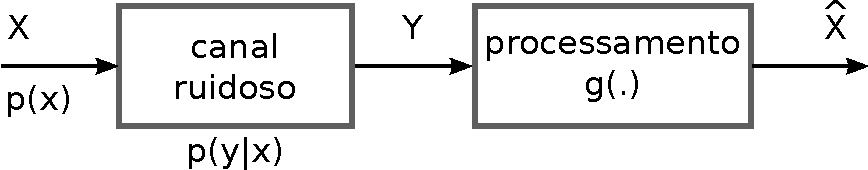
\includegraphics[width=0.7\textwidth]{images/canal-ruidoso.pdf}
  %\caption{.}
  \label{fig:canal-ruidoso}
  \end{figure}

  \begin{itemize}
        \item $\hat{X}$ é uma estimativa de $X$.
        \item a estimativa é errada quando $X \neq \hat{X}$
        \item probabilidade de erro: $P_e \triangleq p(X \neq \hat{X})$
        \item podemos relacionar a entropia condicional $H(X|Y)$ com a probabilidade de erro $P_e$?
        \item sabemos (exercício anterior) que a entropia condicional $H(X|Y)$ é nula se e somente
        se $X$ for uma função de $Y$
        \item esperamos ser capazes de estimar $X$ com baixa probabilidade de erro apenas quando
        a entropia condicional $H(X|Y)$ for pequena
  \end{itemize}
\end{frame}

\subsection{Desigualdade de Fano}

\begin{frame}%[allowframebreaks]
  \frametitle{Desigualdade de Fano}
  \begin{theorem}[Desigualdade de Fano]
  Para qualquer estimador $\hat{X}$ tal que $X \rightarrow Y \rightarrow \hat{X}$, com
  $P_e = Pr(X \neq \hat{X})$, temos
  \begin{equation}
        H(P_e) + P_e \log \left( \vert \mathcal{X} \vert - 1 \right) \geq H(X|\hat{X}) \geq H(X|Y)
  \end{equation}
  Esta desigualdade pode ser simplificada (menos rígida) na forma
  \begin{equation}
  P_e \geq \frac{H(X|Y) - 1}{\log \left( \vert \mathcal{X} \vert - 1 \right)}
  \label{eq:desfanorelax}
  \end{equation}
  onde utilizamos $H(P_e) \leq 1$.
  \end{theorem}
  Note que $P_e = 0 \Rightarrow H(X|Y)=0$ pois $H(P_e)=0$ e $H(X|Y) \geq 0$.
\end{frame}
\note{
Esta desigualdade será utilizada para provar o reverso no teorema de codificação
de Shannon, i.e., que qualquer código com probabilidade de erro $\rightarrow 0$,
à medida que o comprimento do bloco cresce, devemos ter uma taxa $R < C$
(a capacidade do canal, a ser definida).

Para o caso de um alfabeto binário ($\vert \mathcal{X} \vert = 2$),
a desigualdade de Fano na forma da Equação \ref{eq:desfanorelax}
não poderá ser aplicada. Devemos então utilizar a forma mais relaxada:
  \begin{equation}
  P_e \geq \frac{H(X|Y) - 1}{\log \left( \vert \mathcal{X} \vert - 1 \right)} 
        > \frac{H(X|Y) - 1}{\log \vert \mathcal{X} \vert }
  \end{equation}

}

\begin{frame}[allowframebreaks]
  \frametitle{Desigualdade de Fano}
  \begin{proof}
        Definir uma função de erro:
        \begin{equation}
        E = \begin{cases} 1 &, \text{ se } \hat{X} \neq X \text{(erro)} \\
                0       &, \text{ se } \hat{X} = X \text{(sem erro)} 
        \end{cases}
        \end{equation}

        \proofbreak

        Utilizando a regra da cadeia temos:
        \vspace{-0.3cm}
        \begin{eqnarray}
        H(E,X|\hat{X}) &=& H(X|\hat{X}) + \underbrace{H(E|X,\hat{X})}_{=0} \nonumber \\
                        &\text{ou}& \nonumber \\
                        &=& \underbrace{H(E|\hat{X})}_{\leq H(E) = H(P_e)} + \underbrace{H(X|E,\hat{X})}_{\leq P_e \log (\vert \mathcal{X} \vert - 1)}
        \end{eqnarray}
        \vspace{-0.3cm}
        \begin{itemize}
        \item O erro é uma função determinística de $X$ e $\hat{X}$, então, sabendo $X$ e $\hat{X}$,
                determinamos $E$. Desta forma: $H(E|X,\hat{X})=0$.
        \item Condicionar só pode reduzir a entropia: $H(E|\hat{X}) \leq H(E) = H(P_e)$.
        \item Veremos abaixo que $H(X|E,\hat{X}) \leq P_e \log (\vert \mathcal{X} \vert - 1)$.
        \end{itemize}

        \proofbreak

        \vspace{-0.3cm}
        \begin{eqnarray}
        H(X|\hat{X},E) &=& p(E=0) \underbrace{H(X|\hat{X},E=0)}_{=0} + p(E=1)H(X|\hat{X},E=1) \nonumber \\
                        &=& (1-P_e) 0 + P_e H(X|\hat{X},E=1) \leq P_e \log (\vert \mathcal{X} \vert - 1) \nonumber
        \end{eqnarray}
        \begin{itemize}
        \item Se não há erro e conhecemos $\hat{X}$, então determinamos $X$. Não existe entropia 
                residual em $X$ quando é dado $\hat{X}$ e $E=0$. Logo $H(X|\hat{X},E=0)=0$.
        \item Se conhecemos $\hat{X}$ e existe um erro ($E=1$), então sabemos que
                $X$ é diferente de $\hat{X}$, logo isto nos deixa com $(\vert \mathcal{X} \vert - 1)$
                alternativas.
        \end{itemize}

        \proofbreak

        Temos então
        \begin{eqnarray}\label{eq-hhpelog}
        H(X|\hat{X}) &=& H(E|\hat{X}) + H(X|E,\hat{X}) \nonumber \\
                &\leq& H(P_e) + P_e \log (\vert \mathcal{X} \vert - 1)
        \end{eqnarray}

        Como $X \rightarrow Y \rightarrow \hat{X}$ é uma cadeia de Markov, podemos utilizar a
        desigualdade de processamento de dados.
        \begin{eqnarray}\label{hxxhxy}
        I(X;Y) &\geq& I(X;\hat{X}) \nonumber \\
        H(X) - H(X|Y) &\geq& H(X) - H(X|\hat{X}) \nonumber \\
        H(X|\hat{X}) &\geq& H(X|Y)
        \end{eqnarray}

        \proofbreak

        Então, utilizando as Equações \ref{eq-hhpelog} e \ref{hxxhxy}, obtemos
        \begin{equation}
        H(P_e) + P_e \log (\vert \mathcal{X} \vert - 1) \geq H(X|\hat{X}) \geq H(X|Y)
        \end{equation}
        
  \end{proof}
\end{frame}

\begin{frame}%[allowframebreaks]
  \frametitle{Desigualdade de Fano - Sumário}
  Considere a seguinte situação: enviamos $X$ através de um canal ruidoso,
  recebemos $Y$ e realizamos algum pós-processamento.
  \begin{figure}[h!]
  \centering
  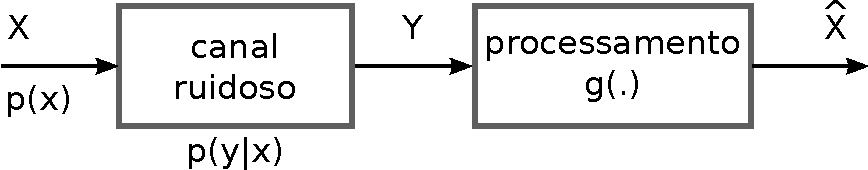
\includegraphics[width=0.8\textwidth]{images/canal-ruidoso.pdf}
  %\caption{.}
  \label{fig:canal-ruidoso}
  \end{figure}
  $\hat{X}$ é uma estimativa de $X$.
  \begin{itemize}
  \item Erro: $X\neq\hat{X}$; com probabilidade $P_e \triangleq p(X\neq \hat{X})$.
  \item Intuitivamente, a entropia condicional deveria nos dizer algo sobre a probabilidade de erro. 
        Na verdade temos o seguinte:
  \end{itemize}

  \begin{theorem}[Desigualdade de Fano]
  \begin{equation}
  H(P_e) + P_e \log (\vert \mathcal{X} \vert -1 ) \geq H(X|\hat{X}) \geq H(X|Y)
  \end{equation}
  \end{theorem}
\end{frame}

\begin{frame}[allowframebreaks]
  \frametitle{Desigualdade de Fano}

  \begin{example}
  Considere uma v.a. discreta $X \in \mathcal{X} = \{1, 2, \ldots, 5\}$ com 
  função massa de probabilidade $p(x) = (0.35, 0.35, 0.1, 0.1, 0.1)$. 
  Seja $Y \in \mathcal{Y} = \{1,2\}$, de forma que, se $x \leq 2$ teremos $y=x$
  com probabilidade $6/7$ e, se $x > 2$, teremos $y=1$ ou $2$ com igual probabilidade.
  A melhor estratégia é utilizar o estimador $\hat{x} = y$. Calcule a probabilidade de erro
  e o limite dado pela desigualdade de Fano.

  \examplebreak

  \textbf{solução}\\
  A distribuição condicional $p(y|x)$ é apresentada na tabela abaixo:
  \begin{center}
  \begin{tabular}{c|cc}
  \diagbox{X}{Y} & 1 & 2 \\
  \hline
  1 & $6/7$  & $1/7$ \\
  2 & $1/7$  & $6/7$ \\
  3 & $1/2$  & $1/2$ \\
  4 & $1/2$  & $1/2$ \\
  5 & $1/2$  & $1/2$
  \end{tabular}
  \end{center}

  \examplebreak

  A efetiva probabilidade de erro é dada por
  \begin{eqnarray}
  P_e &=& 1 - P_a  \ \text{(prob. de acerto)} \nonumber \\
      &=& 1 - \sum_{i=1}^{5} P(x_i = y_i) \nonumber \\
      &=& 1 - \left(  p(y = 1 | x = 1) p(x = 1) + p(y = 2 | x = 2) p(x = 2) + 0 + 0 + 0 \right) \nonumber \\
      &=& 1 - \left( \frac{6}{7} 0.35 + \frac{6}{7} 0.35 \right) = 0.4 = \frac{2}{5}
  \end{eqnarray} 

  \examplebreak

  A desigualdade de Fano fornece um limite inferior pra a probabilidade de erro (predição incorreta do valor de $X$ baseado 
  em $Y$). Este limite inferior é determinado pela incerteza remanescente $H(X|Y)$ sobre $X$ quando $Y$ é conhecido.

  Pelo teorema da desigualdade de Fano temos que
  \begin{equation}
  P_e \geq \frac{H(X|Y) - 1}{\log \left( \vert \mathcal{X} \vert - 1 \right)}
  \end{equation}

  \examplebreak

  Precisaremos calcular 
  \begin{eqnarray}
  H(X|Y) &=& - \sum_{x,y} p(x,y) \log p(x|y) \nonumber \\
         &=& - \sum_{x,y} p(y|x) p(x) \log p(x|y)
  \end{eqnarray}
  onde $p(y|x)$ e $p(x)$ são dados do problema e ainda será necessário calcular $p(x|y)$ para encontrar $H(X|Y)$.

  \examplebreak

  \begin{eqnarray}
  P(X|Y=1) &=& \frac{P(X,Y=1)}{P(Y=1)} = \frac{P(Y=1|X)P(X)}{P(Y=1)} \nonumber \\
        &=& \frac{(\frac{6}{7}, \frac{1}{7}, \frac{1}{2}, \frac{1}{2}, \frac{1}{2}) \cdot (0.35, 0.35, 0.1, 0.1, 0.1) }{ \sum \left( (\frac{6}{7}, \frac{1}{7}, \frac{1}{2}, \frac{1}{2}, \frac{1}{2}) \cdot (0.35, 0.35, 0.1, 0.1, 0.1)  \right)  } \nonumber \\
        &=& \frac{(0.3, 0.05, 0.05, 0.05, 0.05)}{1/2} \nonumber \\
        &=& (0.6, 0.1, 0.1, 0.1, 0.1)
  \end{eqnarray}
  
  \examplebreak

  \begin{eqnarray}
  P(X|Y=2) &=& \frac{(\frac{1}{7}, \frac{6}{7}, \frac{1}{2}, \frac{1}{2}, \frac{1}{2}) \cdot (0.35, 0.35, 0.1, 0.1, 0.1) }{ \sum \left( (\frac{1}{7}, \frac{6}{7}, \frac{1}{2}, \frac{1}{2}, \frac{1}{2}) \cdot (0.35, 0.35, 0.1, 0.1, 0.1)  \right)  } \nonumber \\
        &=& (0.1, 0.6, 0.1, 0.1, 0.1)
  \end{eqnarray}

  \examplebreak 
  
  Desta forma teremos
  \begin{eqnarray}
  H(X|Y) &=& H(X|Y=1) P(Y=1) + H(X|Y=2) P(Y=2) \nonumber \\
        &=& - \frac{1}{2} \left( 0.6 \log 0.6 + 4 \times 0.1 \log 0.1 \right) - \frac{1}{2} \left( 4 \times 0.1 \log 0.1 + 0.6 \log 0.6 \right) \nonumber \\
        &=& 1.771 \text{ bits. }
  \end{eqnarray}

  Utilizando a desigualdade de Fano
  \begin{eqnarray}
  P_e &\geq& \frac{H(X|Y) - 1}{\log \left( \vert \mathcal{X} \vert -1 \right)} = \frac{1.771 - 1}{ \log (5-1)} = 0.3855
  \end{eqnarray}

  \end{example}
\end{frame}

\begin{frame}[allowframebreaks]
  \frametitle{Desigualdade de Fano}
  \begin{lemma}
  Se $X$ e $X'$ são i.i.d. com entropia $H(X)$,
        \begin{equation}
        Pr(X = X') \geq 2^{-H(X)}
        \end{equation}
  com igualdade se e somente se $X$ possuir distribuição uniforme.
  \end{lemma}

  \begin{eqnarray}
  Pr(X = X') &=& Pr(X=x_1|X'=x_1)Pr(X'=x_1) + \ldots + \nonumber \\ && Pr(X=x_n|X'=x_n)Pr(X'=x_n) \nonumber \\
        &=& Pr(X=x_1)Pr(X'=x_1) + \ldots + \nonumber \\ && Pr(X=x_n)Pr(X'=x_n) \nonumber \\
        &=& p^2(x_1) + \ldots + p^2(x_n) = \sum_x p^2(x)
  \end{eqnarray}

  \framebreak

  \begin{proof}
  Suponha que $X \sim p(x)$. Pela desigualdade de Jensen temos
        \begin{equation}
        2^{E[\log p(X)]} \leq E[2^{\log p(X)}]
        \end{equation}
  pois $2^x$ é convexa.
  Logo,
        \begin{eqnarray}
        2^{-H(X)} &=& 2^{\sum_x p(x) \log p(x)} = 2^{E[\log p(X)]} \nonumber \\
                &\leq& E[2^{\log p(X)}] \nonumber \\
                &=& \sum_x p(x) 2^{\log p(x)} = \sum_x p(x)p(x) \nonumber \\
                &=& \sum_x p^2(x) = Pr(X = X')
        \end{eqnarray}
  \end{proof}

  \framebreak
  
  Note que, para maximizar a probabilidade $Pr(X = X')$, devemos minimizar a entropia.
  No limite, quando $H(X)=0$, teremos $Pr(X = X') \geq 1$, logo será igual a $1$ e assim $X = X'$ sem dúvida.
\end{frame}

\begin{frame}[allowframebreaks]
  \frametitle{Desigualdade de Fano}
  \begin{corollary}
  Seja $X, X'$ independentes com $X \sim p(x)$ e $X' \sim q(x)$, $x,x' \in \mathcal{X}$, então
  \begin{eqnarray}
  Pr(X=X') \geq 2^{-H(p) - D(p||q)} \nonumber \\
  Pr(X=X') \geq 2^{-H(q) - D(q||p)}
  \end{eqnarray} 
  ou seja
  \begin{equation}
  Pr(X=X') \geq \max \left( 2^{-H(p) - D(p||q)} , 2^{-H(q)-D(q||p)} \right)
  \end{equation}
  \end{corollary}

  \framebreak

  \begin{proof}
        \begin{eqnarray}
        2^{-H(p) - D(p||q)} &=& 2^{\sum_x p(x) \log p(x) + \sum_x p(x) \log \frac{q(x)}{p(x)}} \nonumber \\
                &=& 2^{\sum_x p(x) \log q(x)} \nonumber \\
                &=& 2^{E_p[\log q(X)]} \nonumber \\
                &\leq& \sum_x p(x) 2^{\log q(x)}  \text{ (Jensen)} \nonumber \\
                &=& \sum_x p(x) q(x) \nonumber \\
                &=& Pr(X=X')
        \end{eqnarray}
  \end{proof}
\end{frame}


% propriedade da equipartição assintótica / conjunto típico
\section{Propriedade da Equipartição Assintótica}

\begin{frame}%[allowframebreaks]
  \frametitle{Propriedade da Equipartição Assintótica}
  \begin{itemize}
  \item Vamos considerar blocos de realizações de uma variável aleatória 
        (i.e., vetores aleatórios de comprimento $n$). $n = \text{tamanho do bloco}$.
  \item Sejam $X_1, X_2, \ldots, X_n$ v.a.s i.i.d. com distribuição $p$ (dizemos
        $X_i \sim p(x)$).
  \item Existem $K$ símbolos possíveis (alfabeto ou espaço-estado de tamanho $K$), então
        $X_i \in \{a_1, a_2, \ldots, a_K\}$.
  \item Consideram $n$ variáveis aleatórias $(X_1, X_2, \ldots, X_n)$, existem $K^n$ possíveis
        realizações.
  \end{itemize}
\end{frame}


\begin{frame}%[allowframebreaks]
  \frametitle{Propriedade da Equipartição Assintótica}
  Suponha que desejamos codificar as $K^n$ possíveis realizações com uma sequência de
  dígitos binários de comprimento $m$. Então, existem $2^m$ palavras de código (\textit{codewords}).
  
  \begin{figure}[h!]
  \centering
  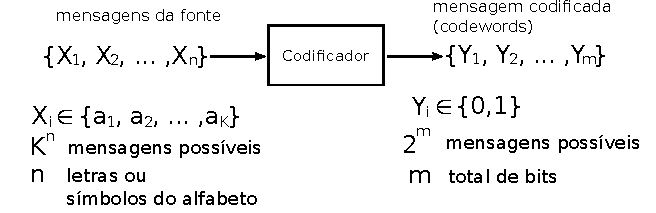
\includegraphics[width=0.7\textwidth]{images/blockcoding.pdf}
  %\caption{.}
  \label{fig:blockcoding}
  \end{figure}
 
  \begin{itemize}
  \item Para que seja possível termos uma palavra de código para cada mensagem possível,
  devemos satisfazer a seguinte condição:
        \begin{equation}
        2^m \geq K^n
        \end{equation}
        ou seja
        \begin{equation}
        m \geq (\log K) n
        \end{equation}
  \end{itemize}
\end{frame}


\begin{frame}%[allowframebreaks]
  \frametitle{Propriedade da Equipartição Assintótica}
  \begin{itemize}
  \item Quantos bits por letra da fonte utilizamos?
        \begin{equation}
        \text{taxa} = \frac{m}{n} \geq \log K \text{ bits por letra da fonte}
        \end{equation}
        Exemplo: 26 letras, precisaremos de $\lceil \log K \rceil = 5 \text{bits}$.
  \item Podemos utilizar menos bits por símbolo emitido pela fonte (na média) e ainda sim
        não ter erro? Sim.
  \item Algumas mensagens da fonte poderiam não ter a elas um código associado.

  \begin{figure}[h!]
  \centering
  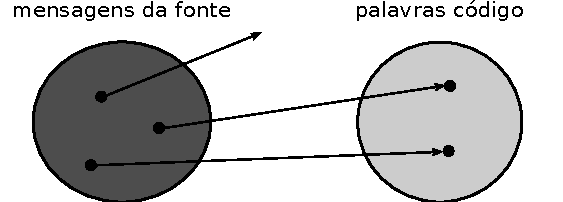
\includegraphics[width=0.5\textwidth]{images/cword-map.pdf}
  %\caption{.}
  \label{fig:cword-map}
  \end{figure}

  \end{itemize}
\end{frame}


\begin{frame}%[allowframebreaks]
  \frametitle{Propriedade da Equipartição Assintótica}
  \begin{itemize}
  \item Ao invés de descartar algumas mensagens, podemos associar a elas palavras longas
        e às outras palavras associamos palavras curtas.

  \begin{figure}[h!]
  \centering   
  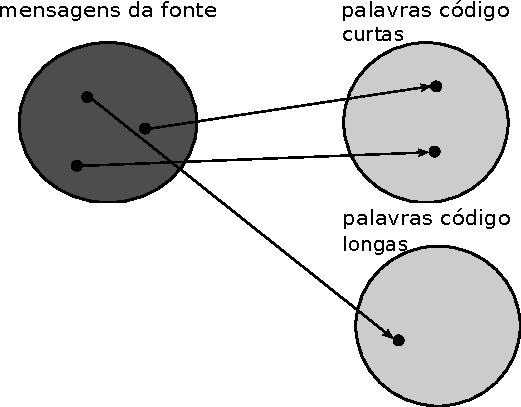
\includegraphics[width=0.35\textwidth]{images/cword-map2.pdf}
  %\caption{.}
  \label{fig:cword-map}
  \end{figure}

  \item Em qualquer um dos casos, quando $n$ é grande suficiente, podemos fazer com que a
        probabilidade, de se obter uma dessas mensagens da fonte que gerariam erro 
        (ou que teriam palavras longas associadas), muito pequena.

  \end{itemize}
\end{frame}


\begin{frame}%[allowframebreaks]
  \frametitle{Probabilidade de Palavras da Fonte}
  \begin{itemize}
  \item A probabilidade de palavras da fonte i.i.d. pode ser expressa por
        \begin{equation}
        p(X_1 = x_1, X_2 = x_2, \ldots, X_n = x_n) = \prod_{i=1}^{n} p(X_i = x_i)
        \end{equation}
  \item A informação (Shannon/Hartley) sobre um evento é dada por $-\log p(x) = I(x)$, então
        \begin{eqnarray}
        I(x_1,x_2,\ldots,x_n) &=& - \log p(x_1, x_2, \ldots, x_n) = - \log \prod_{i=1}^n p(x_i) \nonumber \\
                        &=& \sum_{i=1}^n - \log p(x_i) = \sum_{i=1}^n I(x_i)
        \end{eqnarray}
  \item Eventos independentes são aditivos em relação a esta função de informação.
  \item Note que: $E I(X) = H(X)$.
  \item A lei fraca dos grandes números diz que $\frac{1}{n} S_n \xrightarrow{p} \mu$, onde $S_n$ é a soma
        de v.a.s i.i.d. com média $\mu = E X_i$.
  \item $I(X_i)$ também é uma v.a. com média $H(X)$.
  \end{itemize}
\end{frame}
\note{
\textbf{Lei dos Grandes Números}

Se um evento de probabilidade $p$ é observado repetidamente em ocasiões independentes, 
a proporção da frequência observada deste evento em relação ao total número de repetições 
converge em direção a $p$ à medida que o número de repetições se torna arbitrariamente grande.

\vspace{1cm}

Sejam $X_1, X_2, \ldots, X_n$ v.a.s i.i.d. com $\E X_i = \mu$ e $\Var X_i = \sigma^2 < \infty$, para $i=1,\ldots,n$.
Seja a média definida por $\overline{X_n} = \frac{1}{n} \sum_{i=1}^{n} X_i$, então, para $\varepsilon > 0$,
a \textbf{Lei Fraca dos Grandes Números} diz que $\overline{X_n}$ converge em probabilidade para $\mu$, ou seja,
\begin{equation}
\lim_{n \rightarrow \infty} P \left( \vert \overline{X_n} - \mu \vert < \varepsilon  \right) = 1 .
\end{equation}
}

\begin{frame}%[allowframebreaks]
  \frametitle{Lei fraca dos grandes números e Entropia}
  \begin{itemize}
  \item Combinando o que vimos anteriormente, obtemos
        \begin{equation}
        \frac{1}{n} \sum_{i=1}^n I(X_i) \xrightarrow[n \rightarrow \infty]{p} H(X)
        \end{equation}
  \item Se $n$ fica grande suficiente, obteremos
        \begin{eqnarray}
        \frac{1}{n} \sum_{i=1}^n I(x_i) &\approx& H(X) \text{ onde } \forall i, x_i \sim p(x) \nonumber \\
        - \frac{1}{n} \sum_{i=1}^n \log p(x_i) &\approx& H(X) \nonumber \\
        - \log \prod_{i=1}^n p(x_i) &\approx& n H(X) \nonumber \\
        - \log p(x_1,x_2,\ldots,x_n) &\approx& n H(X) \nonumber \\
        p(x_1,x_2,\ldots,x_n) &\approx& 2^{-nH(X)}
        \end{eqnarray}
  \end{itemize}
\end{frame}

\begin{frame}%[allowframebreaks]
  \frametitle{Propriedade da Equipartição Assintótica}
        Quando $n$ é grande suficiente, teremos
        \begin{equation}
        p(x_1,x_2,\ldots,x_n) \approx 2^{-nH(X)}
        \end{equation}
        
        \begin{itemize}
        \item Esta probabilidade não depende da sequência em si. Depende apenas do comprimento $n$
        e da entropia da v.a.
        \item Quando $n$ fica grande, podemos dizer que todas as sequências terão a mesma probabilidade: $2^{-nH}$.
        \item Estas sequências que possuem esta probabilidade (praticamente todas as sequências) são
        chamadas de sequências \textbf{típicas}, e são representadas pela conjunto $A$.
        \end{itemize}
\end{frame}

\begin{frame}%[allowframebreaks]
  \frametitle{Quase todos eventos são quase equiprováveis}
  \begin{itemize}
  \item Se $X_1,X_2,\ldots,X_n$ são i.i.d. e $X_i \sim p(x)$ para todo $i$, e se $n$ é grande suficiente, 
        então qualquer amostra $x_1,x_2,\ldots,x_n$ terá 
        probabilidade da amostra essencialmente independente da amostra, i.e.,
        \begin{equation}
        p(x_1,\ldots,x_n) \approx 2^{-nH(X)}
        \end{equation}
        onde $H(X)$ é a entropia de $p(x)$.
  \item Então, podem existir no máximo $2^{nH}$ amostras, e pode ser que $2^{nH} \ll K^n$.
  \item Estas amostras que ocorrem são chamadas de típicas, e são representadas por $A_\epsilon^{(n)}$.
  \item Uma grande porção de $\mathcal{X}^n$ não irá ocorrer, i.e., pode acontecer que 
        $2^{nH} \ll \vert \mathcal{X}^n \vert = K^n$.
  \end{itemize}
\end{frame}

\begin{frame}%[allowframebreaks]
  \frametitle{Conjunto Típico}
  \begin{itemize}
  \item Seja $A_\epsilon^{(n)}$ o conjunto das sequências típicas (i.e., aquelas com probabilidade $2^{-nH}$).
  \item Se ``todos'' eventos possuem a mesma probabilidade $p$, então existem $1/p$ deles.
  \item O número de sequências típicas é
        \begin{equation}
        \vert A_\epsilon^{(n)} \vert \approx 2^{nH(X)}.
        \end{equation}
  \item Desta forma, para representar (ou codificar) as sequencias típicas, precisaremos de
        $nH(X)$ bits. Teremos então
        \begin{equation}
        m = nH(X)
        \end{equation}
        no modelo do codificador. Então a taxa será $H(X)$.
  \end{itemize}

\end{frame}


\begin{frame}%[allowframebreaks]
  \frametitle{Codificando apenas o Conjunto Típico}
  \begin{itemize}
  \item Tomando $m=nH$, teremos que o número médio de bits por letra do alfabeto da fonte será dado por
        \begin{equation}
        \frac{m}{n} = H         \text{  que pode ser } \leq \log K
        \end{equation}
  \item Interpretações para a Entropia na codificação de fonte:
        \begin{enumerate}
        \item A probabilidade de uma sequência típica é $2^{-nH(X)}$.
        \item O número de sequências típicas é $2^{nH(X)}$.
        \item O número de bits por símbolo da fonte é $H(X)$, quando codificamos apenas o conjunto típico.
        \end{enumerate}
  \end{itemize}
\end{frame}


\begin{frame}%[allowframebreaks]
  \frametitle{Bernoulli}
  Considere o experimento de Bernoulli com $X_1,\ldots,X_n$ i.i.d. e probabilidade
  $p(X_i=1)=p=1-p(X_i=0)$. A probabilidade de uma dada sequência será dada por
  \begin{equation}
  p(x_1,x_2,\ldots,x_n) = \prod_{i=1}^n p^{x_i} (1-p)^{1-x_i} = p^{\sum_i x_i} (1-p)^{n - \sum_i x_i}
  \end{equation}

  \begin{itemize}
  \item Existem $2^n$ sequencias possíveis.
  \item Todas elas possuem a mesma probabilidade? Não. Considere $p=0.1$, $(1-p)=0.9$.
        A sequência de apenas zeros é a sequência de mais provável.
  %\item Qual é a sequência mais provável? Quando $p=0.1$, será a sequência com apenas zeros.
  \end{itemize}
\end{frame}
\note{
  Todas as sequências que possuem `alguma' probabilidade, terão a mesma probabilidade?
  Depende do que queremos dizer com `alguma'. Para valores pequenos de $n$, não, mas à medida
  que $n$ cresce, algo acontece e a resposta `sim' começa a ser a mais apropriada. 
}

\begin{frame}%[allowframebreaks]
  \frametitle{Propriedade de Equipartição Assintótica}
  \begin{itemize}
  \item É possível prever a probabilidade de que uma determinada sequências terá uma probabilidade particular?
        \begin{equation}
        \Pr(p(X_1,X_2,\ldots,X_n)=\alpha) = ?
        \end{equation}
  \item Note que $p(X_1,X_2,\ldots,X_n)$ é uma variável aleatória. É uma probabilidade que é uma função
        do conjunto de variáveis aleatórias.
  \item Teremos
        \begin{equation}
        \Pr(p(X_1,X_2,\ldots,X_n) \approx 2^{-nH} ) \approx 1
        \end{equation}
        quando $n$ é grande suficiente.
  \item Quase todos os eventos (que ocorrem com alguma probabilidade) são todos equiprováveis.
  \end{itemize}
\end{frame}

\begin{frame}%[allowframebreaks]
  \frametitle{Ensaio de Bernoulli}
  \begin{example}
  Seja $S_n \sim \text{Binomial}(n,p)$ com $S_n = X_1 + X_2 + \ldots + X_n$, $X_i \sim \text{Bernoulli}(p)$.
  Teremos então $ES_n = np$ e $\text{var}(S)=npq$, onde $q=1-p$, e
        \begin{equation}
        p(S_n = k) = {n \choose k} p^k q^{n-k}
        \end{equation}
  Analisando a expressão para $2^{-nH}$, temos
        \begin{eqnarray}
        2^{-nH(p)} &=& 2^{-n(-p \log p - (1-p)\log(1-p))} \nonumber \\
                &=& 2^{\log p^{np} + \log(1-p)^{n(1-p)}} \nonumber \\
                &=& p^{np}q^{nq}
        \end{eqnarray}
  $H=H(p)$ é a entropia binária com probabilidade $p$.
  $np$ é o número esperado de $1$s e $nq$ é o número esperado de $0$s.
  \end{example}
\end{frame}
\note{
        \begin{itemize}
        \item Todas as sequências que ocorrem são aquelas cujo número de $1$s e $0$s são
                aproximadamente iguais aos seus valores esperados.
        \item Nenhum outra sequência possui probabilidade significativa.
        \item A sequência $X_1, X_2, \ldots, X_n$ foi assumida como sendo i.i.d., entretanto
                podemos estender para cadeias de Markov e processos aleatórios estacionários ergódicos.
        \end{itemize}
}
\note{
O cálculo computacional do coeficiente binomial pode apresentar perda de precisão numérica, por envolver
fatoriais e frações de números muito grandes. Exemplo de execussão no GNU-Octave para calcular ${100 \choose 20}$:
\begin{semiverbatim}
>> nchoosek(100,20)

warning: nchoosek: possible loss of precision

warning: called from
\end{semiverbatim}
Uma possível solução é utilizar o pacote simbólico para efetuar os cálculos. 
Podemos verificar que realmente ocorreu erro de precisão numérica ao realizar o cálculo computacional.
\begin{semiverbatim}
>> double(nchoosek(sym(100),sym(20))) - nchoosek(100,20)

ans = -65536
\end{semiverbatim}
}
\note{
Outra alternativa é realizar uma aproximação para calcular ${N \choose k}$.

Iremos utilizar a aproximação de Stirling para a função fatorial:
\begin{equation}
\ln n! =  n \ln n - n + \mathcal{O}(\ln n) 
\end{equation}
%\begin{equation}
%\ln x! \simeq x \ln x - x + \frac{1}{2} \ln 2 \pi x .
%\end{equation}
Utilizando esta aproximação em $\ln {N \choose k}$, teremos
\begin{eqnarray}
\ln {N \choose k} &\equiv& \ln \frac{N!}{(N-k)!k!} = \ln N! - \ln (N-k)! - \ln k! \nonumber \\
        &\simeq& N \ln N - N - (N-k) \ln (N-k) + (N-k) - k \ln k + k \nonumber \\
        &=& \underbrace{(N-k)\ln N - (N-k)\ln N}_{=0} + N \ln N - N - (N-k) \ln (N-k) + (N-k) - k \ln k + k \nonumber \\
        &=& (N-k)\ln \frac{N}{N-k} + k \ln \frac{N}{k}  \nonumber \\
        &=& N \left( -\frac{N-k}{N} \ln \frac{N-k}{k} - \frac{k}{N} \ln \frac{k}{N} \right) = N H_e\left(\frac{k}{N}\right) .
%\frac{N \ln N - N + \frac{1}{2} \ln 2\pi N}{ \left( (N-k) \ln (N-k) - (N-k) + \frac{1}{2} \ln 2\pi (N - k) \right) \left( k \ln k - k + \frac{1}{2} \ln 2\pi k \right) }
\end{eqnarray}
}
\note{
Concluímos então que
\begin{equation}
\ln {N \choose k} \simeq N H_e\left(\frac{k}{N}\right)
\end{equation}
e, como os temos em ambos os lados envolvem logaritmos, podemos realizar a mudança de base em ambos os lados
(basta multiplicar por $\ln 2$),
\begin{equation}
\log {N \choose k} \simeq N H \left(\frac{k}{N}\right) ,
\end{equation}
onde agora utilizamos a entropia binária em bits. Assim, teremos
\begin{equation}
{N \choose k} \simeq 2^{N H \left(\frac{k}{N}\right)} .
\end{equation}

}


\begin{frame}%[allowframebreaks]
  \frametitle{Propriedade da Equipartição Assintótica}
  \begin{theorem}[Propriedade da Equipartição Assintótica]\label{thm-prop-eqp-ass}
        Se $X_1, X_2, \ldots, X_n$ são i.i.d. e $X_i \sim p(x)$ para todo $i$, então
        \begin{equation}\label{eq-pX1X2Xn-H}
        -\frac{1}{n} \log p(X_1, X_2, \ldots, X_n) \xrightarrow{p} H(X)
        \end{equation}
  \end{theorem}

  \begin{proof}
  \vspace{-2ex}
  \begin{eqnarray}
  -\frac{1}{n} \log p(X_1, X_2, \ldots, X_n) &=& - \frac{1}{n} \log \prod_{i=1}^n p(X_i) \nonumber \\
                &=& - \frac{1}{n} \sum_i \log p(X_i) \xrightarrow{p} E \log p(X) \nonumber \\
                && \text{\scriptsize onde utilizamos a lei fraca dos números grandes} \nonumber \\
                &=& H(X)
  \end{eqnarray}
  \end{proof}
\end{frame}


\begin{frame}%[allowframebreaks]
  \frametitle{Conjunto Típico}
  \begin{definition}[Conjunto Típico]
  Um conjunto típico $A_\epsilon^{(n)}$ em relação a $p(x)$ é o conjunto de sequências 
  $(x_1,x_2,\ldots,x_n) \in \mathcal{X}^n$ com propriedade
        \begin{equation}
        2^{-n(H(X)+\epsilon)} \leq p(x_1, x_2, \ldots, x_n) \leq 2^{-n(H(X)-\epsilon)}
        \end{equation}
  De forma equivalente, podemos escrever
        \begin{equation}
        A_\epsilon^{(n)} = \left\{ (x_1, x_2, \ldots, x_n) : \vert - \frac{1}{n} \log p(x_1, \ldots, x_n) - H \vert < \epsilon \right\}
        \end{equation}
  \end{definition}

  O conjunto típico é formado pelas sequências com $\log$ da probabilidade dentro
  de seguinte extensão 
  \begin{figure}[h!]
  \centering
  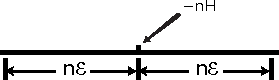
\includegraphics[width=0.35\textwidth]{images/range-ts.pdf}
  %\caption{.}
  \label{fig:range-ts}
  \end{figure}
\end{frame}


\begin{frame}%[allowframebreaks]
  \frametitle{Conjunto Típico}
  \begin{itemize}
  \item O tamanho do conjunto típico de sequências produzidas pela fonte é tipicamente
        muito menor que o tamanho do conjunto de todas as sequências produzidas pela fonte.
  \item Uma sequencia típica não precisa ter probabilidade próxima daquela que é a sequência mais provável.
  \item Geralmente a sequência mais provável não está no conjunto típico.
  \end{itemize}
\end{frame}



\subsection{Propriedades do Conjunto Típico}
\begin{frame}%[allowframebreaks]
  \frametitle{Propriedades do Conjunto Típico}
  \begin{theorem}[Propriedades do Conjunto Típico $A_\epsilon^{(n)}$]
  \begin{enumerate}
  \item Se $(x_1, x_2, \ldots, x_n) \in A_\epsilon^{(n)}$, então
        \begin{equation}
        H(X) - \epsilon \leq - \frac{1}{n} \log p(x_1, x_2, \ldots, x_n) \leq H(X) + \epsilon
        \end{equation}
  \item $p(A_\epsilon^{(n)}) = p\left( \left\{ x: x \in A_\epsilon^{(n)} \right\} \right) > 1 - \epsilon$ para $n$ grande suficiente, para todo $\epsilon > 0$.
  \item Limite superior: $\vert A_\epsilon^{(n)} \vert \leq 2^{n(H(X)+\epsilon)}$, onde $\vert A_\epsilon^{(n)} \vert$ é o número de elementos no conjunto $A_\epsilon^{(n)}$.
  \item Limite inferior: $\vert A_\epsilon^{(n)} \vert \geq (1-\epsilon) 2^{n(H(X) - \epsilon)}$ para $n$ grande suficiente.
  \end{enumerate}
  \end{theorem}

  \begin{itemize}
  \item O conjunto típico possui, essencialmente, probabilidade $1$ (algo típico irá tipicamente ocorrer).
  \item Todos os itens neste conjunto terão a mesma probabilidade $\approx 2^{-nH}$.
  \end{itemize}
\end{frame}

\begin{frame}%[allowframebreaks]
  \frametitle{Exemplo $K=\vert \{0,1\} \vert$: Conjunto Típico}
  \begin{itemize}
  \item Suponha o Ensaio de Bernoulli com distribuição uniforme, $K=2$, 
        $\mathcal{X} = \{0,1\}$, $p=0.5$, entropia $H=1$ e
        $\vert A_\epsilon^{(n)} \vert = 2^{nH} = 2^n = K^n$, 
        então todas as sequências ocorreram com igual probabilidade.
  \item Considere agora uma distribuição não-uniforme, $p=0.1$ e $q=1-p=0.9$, a entropia será
        $H\approx 0.469$. Considere $n=100$, então 
        $K^{100} = 2^{100} = 10^{\log_{10} 2^{100}} \approx 10^{100 \times 0.30103} \approx 10^{30}$,
        a capacidade representacional das sequencias da fonte. 
        Mas $\vert A_\epsilon^{(n)} \vert = 2^{nH} = 10^{nH \times \log_{10} 2} \approx 10^{14} \ll 10^{30} \approx K^{100}$. 
        O número de sequências típicas é muito menor que o número de possíveis sequências.
  \item Ineficiência: capacidade representacional é muito maior do que as coisas que ocorrem.
        O alfabeto da fonte é pobre para realizar compressão.
  \item Assuma $\epsilon$ muito pequeno, então onde foi parar a massa das $\approx 10^{30} - 10^{14}$ 
        sequencias? (veremos adiante)
  \end{itemize}
\end{frame}


\begin{frame}%[allowframebreaks]
  \frametitle{Conjunto Típicos são Típicos}
  \begin{itemize}
  \item Pela definição
        \begin{equation}
        p(A_\epsilon^{(n)}) > 1 - \epsilon \text{ para qualquer } \epsilon > 0
        \end{equation}
  \item Então $A_\epsilon^{(n)}$ possui praticamente toda probabilidade, e cada elemento
        em $A_\epsilon^{(n)}$ possui a mesma probabilidade, então
        \begin{equation}
        p(x) \approx 2^{-nH} \forall x \in A_\epsilon^{(n)}
        \end{equation}
  \item Exemplo: Ensaio de Bernoulli $X_i \sim \text{Bernoulli}(p)$ com 
        $p(X_i = 1) = p = 1 - p(X_i = 0)$ e $p>0.5$.
  \item Probabilidade de $n$ $1$s sucessivos é $p^n$ e esta é a sequência mais provável.
  \item Probabilidade de uma sequência típica é $2^{-nH}$.
  \item Para $n=100$, $p-0.9 = 1 - q$, a sequência mais provável possui probabilidade
        $p^n \approx 2.66 \times 10^{-5}$, mas uma sequencia típica possui probabilidade
        $2^{-nH} \approx 7.62 \times 10^{-15}$.
  \end{itemize}
\end{frame}

\begin{frame}%[allowframebreaks]
  \frametitle{Exemplo $K=\vert \{0,1\} \vert$: Conjunto Típico}
  \begin{itemize}
  \item Suponha o Ensaio de Bernoulli com distribuição uniforme, $K=2$, 
        $\mathcal{X} = \{0,1\}$, $p=0.5$, entropia $H=1$ e
        $\vert A_\epsilon^{(n)} \vert = 2^{nH} = 2^n = K^n$, 
        então todas as sequências ocorreram com igual probabilidade.
  \item Considere agora uma distribuição não-uniforme, $p=0.1$ e $q=1-p=0.9$, a entropia será
        $H\approx 0.469$. Considere $n=100$, então 
        $K^{100} = 2^{100} = 10^{\log_{10} 2^{100}} \approx 10^{100 \times 0.30103} \approx 10^{30}$,
        a capacidade representacional das sequencias da fonte. 
        Mas $\vert A_\epsilon^{(n)} \vert = 2^{nH} = 10^{nH \times \log_{10} 2} \approx 10^{14} \ll 10^{30} \approx K^{100}$. 
        O número de sequências típicas é muito menor que o número de possíveis sequências.
  \item Ineficiência: capacidade representacional é muito maior do que as coisas que ocorrem.
        O alfabeto da fonte é pobre para realizar compressão.
  \item Assuma $\epsilon$ muito pequeno, então onde foi parar a massa das $\approx 10^{30} - 10^{14}$ 
        sequencias? (veremos adiante)
  \end{itemize}
\end{frame}

\begin{frame}%[allowframebreaks]
  \frametitle{Conjunto Típicos são Típicos}
  \begin{itemize}
  \item Pela definição
        \begin{equation}
        p(A_\epsilon^{(n)}) > 1 - \epsilon \text{ para qualquer } \epsilon > 0
        \end{equation}
  \item Então $A_\epsilon^{(n)}$ possui praticamente toda probabilidade, e cada elemento
        em $A_\epsilon^{(n)}$ possui a mesma probabilidade, então
        \begin{equation}
        p(x) \approx 2^{-nH} \forall x \in A_\epsilon^{(n)}
        \end{equation}
  \item Exemplo: Ensaio de Bernoulli $X_i \sim \text{Bernoulli}(p)$ com 
        $p(X_i = 1) = p = 1 - p(X_i = 0)$ e $p>0.5$.
  \item Probabilidade de $n$ $1$s sucessivos é $p^n$ e esta é a sequência mais provável.
  \item Probabilidade de uma sequência típica é $2^{-nH}$.
  \item Para $n=100$, $p-0.9 = 1 - q$, a sequência mais provável possui probabilidade
        $p^n \approx 2.66 \times 10^{-5}$, mas uma sequencia típica possui probabilidade
        $2^{-nH} \approx 7.62 \times 10^{-15}$.
  \end{itemize}
\end{frame}

\begin{frame}%[allowframebreaks]
  \frametitle{Sequencias Não-Típicas não são típicas}
  \begin{itemize}
  \item $p^n \gg 2^{-nH}$: a sequência mais provável é muito mais provável do que uma 
        sequencia típica.
  \item O que ocorre com a probabilidade da sequencia mais provável, na média (por símbolo),
        quando $n$ cresce
        \begin{equation}
        - \frac{1}{n} \log p^n = - \log p = \log 1/p \xrightarrow[n \rightarrow \infty] p H ?
        \end{equation} 
  \item O conjunto típico possui, essencialmente, toda a probabilidade $p(A_\epsilon^{(n)}) > 1 - \epsilon $.
  \item A sequencia mais provável está no conjunto típico? 
        Não, já que a probabilidade da sequencia mais provável não é $2^{-nH}$.
  \item $n=100$, $p=0.9=1-q$. Considere uma sequência com noventa $1$s e dez $0$s.
        A probabilidade é $p^{90}(1-p)^{10} \approx 7.62 \times 10^{-15} \approx 2^{-nH}$.
  \item Esta sequencia muito improvável é típica.
  \end{itemize}
\end{frame}

\begin{frame}%[allowframebreaks]
  \frametitle{Probabilidade Média de Sequencias}
  \begin{itemize}
  \item Pela PEA (Propriedade da Equipartição Assintótica), temos que se 
        $(x_1, \ldots, x_n)$ é típico (i.e., $(x_1, \ldots, x_n) \in A_\epsilon^{(n)}$, 
        para qualquer $\epsilon > 0$), então
        \begin{equation}
        - \frac{1}{n} \log p(x_1, \ldots, x_n) \xrightarrow[n \rightarrow \infty]{p} H 
        \end{equation}
  \item Para as sequencias mais prováveis, quando $n$ é grande suficiente, teremos (para $p>0.5$)
        \begin{equation}
        - \frac{1}{n} \log p^n = - \log p = \log 1/p \xrightarrow[n \rightarrow \infty]{p} - \log p
        \end{equation}
  \item A probabilidade média da sequencia mais provável é bem diferente da sequencia típica.
  \end{itemize}
\end{frame}

\begin{frame}%[allowframebreaks]
  \frametitle{Sequencias Típicas}
  \begin{itemize}
  \item o conjunto típico possui essencialmente toda da probabilidade.
  \item Como pode uma sequencia com a maior probabilidade não ser típica,
        mas uma sequência com probabilidade muito menor ser típica?
  \item Existe um número exponencialmente crescente de sequencias típicas, cada uma
        com probabilidade menor do que a sequencia de maior probabilidade.
  \item A probabilidade individual de cada sequencia vai a zero quando $n$ cresce.
  \item O tamanho do conjunto típico cresce rapidamente, quando $n \rightarrow \infty$,
        de forma que a probabilidade de $A_\epsilon^{(n)}$ vai a $1$.
  \item O tamanho do conjunto das sequencias muito prováveis cresce lentamente, de forma
        que a probabilidade do conjunto vai a zero quando $n \rightarrow \infty$. 
  \end{itemize}
\end{frame}

\begin{frame}[allowframebreaks]
  \frametitle{Sequencias Típicas} 
  A probabilidade de uma sequência $x_{1:n}$, onde $x_i \in \mathcal{X} = \{a_1, \ldots, a_K\}$, é dada por
  \begin{equation}
  P(x_{1:n}) = P(x_1) P(x_2) \ldots P(x_n) \approx p_1^{p_1 n} p_2^{p_2 n} \ldots p_K^{p_K n} ,
  \end{equation}
  onde consideramos que, em uma sequência muito longa, esperamos observar $p_1 n$ ocorrências do símbolo $a_1$,
  $p_2 n$ ocorrências do símbolo $a_2$, etc.

  A informação associada a esta sequência típica é
  \begin{eqnarray}
  \log \frac{1}{P(x_{1:n})} &\approx& \sum_{i=1}^K \log p_i^{-p_i n} \\
                &=& n \sum_{i=1}^K p_i \log \frac{1}{p_i} = n H(X).
  \end{eqnarray}
  Uma sequência típica terá probabilidade próxima de $2^{-n H(X)}$.

  \framebreak
  \begin{figure}[h!]
  \centering
  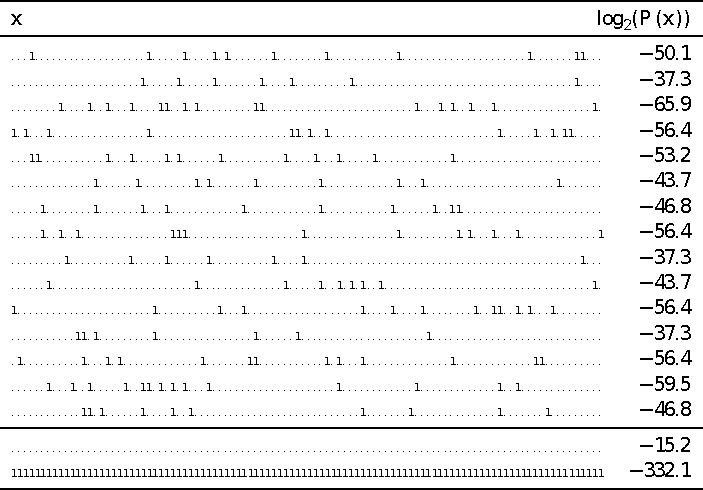
\includegraphics[width=0.5\textwidth]{images/seq100mackay.pdf}
  \caption{Sequências regadas por um ensaio de Bernoulli com $n=100$ e $P(X=1) = p = 0.1$. 
        As 15 sequências superiores representam amostras típicas. As duas últimas sequências
        representam a sequência mais provável e a menos provável \cite{mackay2003}.}
  \label{fig:seq100mackay}
  \end{figure}

  \framebreak
  \begin{figure}[h!]
  \centering
  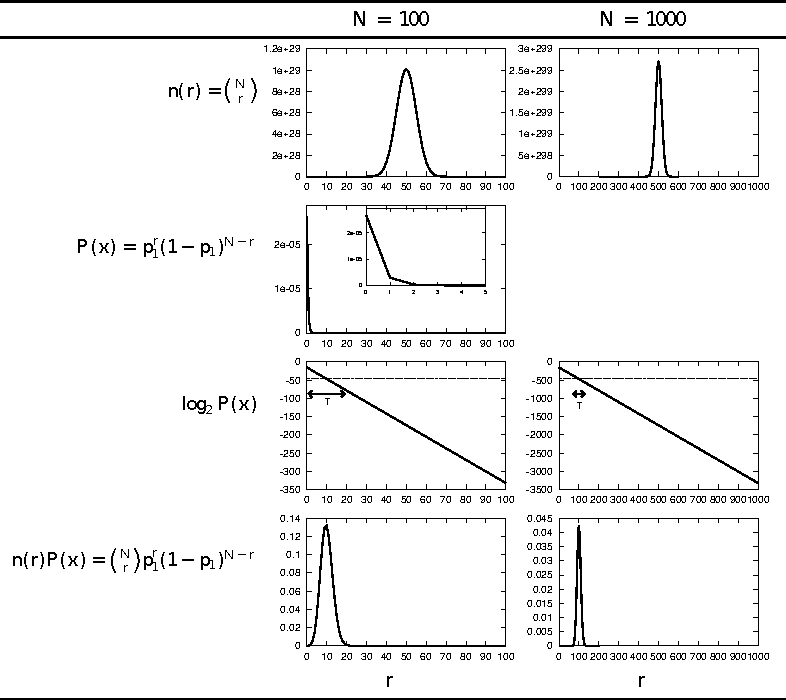
\includegraphics[width=0.5\textwidth]{images/seq100mackay2.pdf}
  \caption{Para $p=0.1$, $n=100$ e $n=1000$ os gráficos ilustram $n(r)$, o número de strings contendo
        $r$ 1s; a probabilidade $P(x_{1:n})$ para uma string contendo $r$ 1s; a mesma probabilidade
        em escala logarítmica; e a probabilidade total $n(r) P(x_{1:n})$ de todas as strings contendo $r$ 1s \cite{mackay2003}.}
  \label{fig:seq100mackay2}
  \end{figure}


  \framebreak
  \begin{figure}[h!]
  \centering
  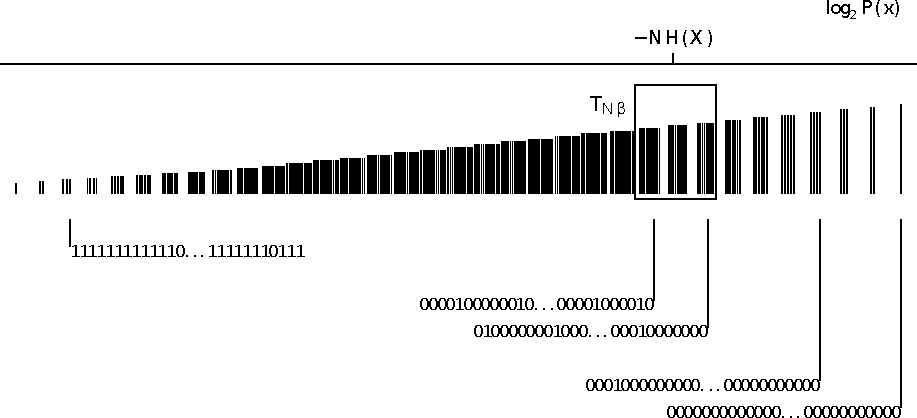
\includegraphics[width=0.5\textwidth]{images/seq100mackay3.pdf}
  \caption{Diagrama esquemático ilustrando todas as sequencias no conjunto $\mathcal{X}^n$ ordenadas pela probabilidade \cite{mackay2003}.}
  \label{fig:seq100mackay3}
  \end{figure}


  O termo \textbf{equipartição} é utilizado para descrever a ideia de que os membros do conjunto típico
  possuem aproximadamente a mesma probabilidade.

  
\end{frame}


\subsection{Exercícios}
\begin{frame}[allowframebreaks]
  \frametitle{Exercício 1}

  \begin{exercise}[Desigualdade de Markov e Desigualdade de Chebyshev]
  \begin{enumerate}[a)]
  \item \emph{(Desigualdade de Markov)} Para qualquer v.a. não negativa $X$ e qualquer $\delta > 0$, mostre que
	\begin{equation}
	\Pr \left( X \geq \delta \right) \leq \frac{\E X}{\delta} .
	\end{equation} 
 	Mostre uma v.a. para a qual teremos igualdade na equação acima.
  \end{enumerate}

  \exercisebreak

  \textbf{solução}: 
  Se $X$ possui distribuição $f(x)$, então
  \begin{eqnarray}
  \E X &=& \int_0^\infty x f(x) \mathrm{d}x = \int_0^\delta x f(x) \mathrm{d}x + \int_\delta^\infty x f(x) \mathrm{d}x \nonumber \\
	&\geq& \int_\delta^\infty x f(x) \mathrm{d}x \nonumber \\
	&\geq& \int_\delta^\infty \delta f(x) \mathrm{d}x \nonumber \\
	&=& \delta \Pr \left( X \geq \delta \right) .
  \end{eqnarray}

  \exercisebreak
  Podemos assim concluir que
  \begin{equation}
  \Pr \left( X \geq \delta \right) \leq \frac{\E X}{\delta} .
  \end{equation}


  \exercisebreak
  \begin{enumerate}[b)]
  \item \emph{(Desigualdade de Chebyshev)} 
	Seja $Y$ uma v.a. com média $\mu$ e variância $\sigma^2$. Façamos $X = (Y - \mu)^2$.
	Mostre que para qualquer $\varepsilon > 0$, 
	\begin{equation}
	\Pr \left( \vert Y - \mu \vert > \varepsilon \right) \leq \frac{\sigma^2}{\varepsilon^2} .
	\end{equation}
  \end{enumerate}

  \exercisebreak

  \textbf{solução}:

  Utilizando a desigualdade de Markov com $X = (Y - \mu)^2$ e $\delta = \varepsilon^2$, temos
  \begin{equation}
  \Pr \left( (Y-\mu)^2 \geq \varepsilon^2 \right) \leq \frac{\E (Y-\mu)^2}{\varepsilon^2} = \frac{\sigma^2}{\varepsilon^2}
  \end{equation}
  Vamos utilizar também que $\Pr \left( (Y-\mu)^2 > \varepsilon^2 \right) \leq \Pr \left( (Y-\mu)^2 \geq \varepsilon^2 \right)$
  e $\Pr \left( (Y-\mu)^2 > \varepsilon^2 \right) = \Pr \left( \vert Y - \mu \vert > \varepsilon \right)$. Assim teremos
  \begin{equation}
  \Pr \left( \vert Y - \mu \vert > \varepsilon \right) \leq \frac{\sigma^2}{\varepsilon^2} ,
  \end{equation}
  como queríamos demonstrar.

  \exercisebreak
  \begin{enumerate}[c)]
  \item \emph{(Lei fraca dos grandes números)}
  Seja $Z_1, Z_2, \ldots, Z_n$ uma sequência de v.a. i.i.d. com média $\mu$ e variância $\sigma^2$.
  Seja $\overline{Z_n} = \frac{1}{n} \sum_{i=1}^{n} Z_i$, a média amostral. Mostre que
  \begin{equation}
  \Pr \left( \vert \overline{Z_n} - \mu \vert > \varepsilon \right) \leq \frac{\sigma^2}{n \varepsilon^2} .
  \end{equation}
  Então teremos $\Pr \left( \vert \overline{Z_n} - \mu \vert > \varepsilon \right) \rightarrow 0$ quando 
  $n \rightarrow \infty$, sendo esta a lei fraca dos grandes números.
  \end{enumerate}

  \exercisebreak

  \textbf{solução}:

  Vamos utilizar a desigualdade de Chebyshev com $Y = \overline{Z_n}$, observado que 
  $\E \overline{Z_n} = \mu$ e $\Var (\overline{Z_n}) = \frac{\sigma^2}{n}$
  (i.e. $\overline{Z_n}$ é a soma de $n$ v.a. i.i.d. $\frac{Z_i}{n}$, cada uma com 
  variância $\frac{\sigma^2}{n^2}$). Teremos assim
  \begin{equation}
  \Pr \left( \vert \overline{Z_n} - \mu \vert > \varepsilon  \right) \leq \frac{\sigma^2}{n \varepsilon^2} .
  \end{equation}

  A desigualdade de Chebyshev é utilizada para provar a propriedade da equipartição assintótica (ver teorema \ref{thm-prop-eqp-ass}).
  \end{exercise}
% ver pg 82 Mackay
\end{frame}


\begin{frame}[allowframebreaks]
  \frametitle{Exercício 7}
  \begin{exercise}[PEA e codificação de fonte]
  Uma fonte discreta sem memória emite uma sequência binária de dígitos independentes com 
  probabilidade $p(1)=0.005$ e $p(0) = 0.995$. Os dígitos são tomados em grupo de 100 e 
  uma palavra binária é fornecida para cada sequência de 100 dígitos contendo três ou menos uns.

  \exercisebreak
  \begin{enumerate}[a)]
  \item Assumindo que todas as palavras código possuem a mesmo comprimento, encontre o comprimento mínimo
	necessário para fornecer código para todas as sequências com três ou menos uns (1s).
  \end{enumerate}

  \textbf{solução}
 
  O número de sequências binárias de 100 bits com três ou menos uns é dado por
  \begin{equation}
  {100 \choose 0} + {100 \choose 1} + {100 \choose 2} + {100 \choose 3} = 1 + 100 + 4950 + 161700 = 166751
  \end{equation}
  \exercisebreak
  Considerando que os códigos terão todos o mesmo comprimento, que deverá ser 
  $\lceil \log 166751 \rceil = 18$. Note que $H(0.005) = 0.0454$, logo para uma sequência de 100 símbolos
  teremos $4.5$ bits de entropia, que é bem menor do que os 18 bits encontrados.


  \exercisebreak
  \begin{enumerate}[b)]
  \item Calcule a probabilidade de observar uma sequência da fonte para a qual nenhum código foi atribuído.
  \end{enumerate}
  \textbf{solução}
  
  Devemos considerar aqui as sequências com mais de 3 uns. A probabilidade observarmos uma sequência para a
  qual não existe código associado é igual a um menos a probabilidade de observármos uma sequência para a 
  qual existe código associado, ou seja,
  \begin{equation}
  1 - \sum_{i=0}^{3} {100 \choose i} (0.005)^i (0.995)^{100-i} = 1 - 0.60577 - 0.30441 - 0.01243 = 0.00167.
  \end{equation}


  \exercisebreak
  \begin{enumerate}[c)]
  \item Use a desigualdade de Chebyshev para limitar a probabilidade de observamos um sequencia da fonte
	para a qual nenhum código foi associado. Compare este limite com o valor calculado no item anterior.
  \end{enumerate}
  \textbf{solução}

  Para a v.a. $S_n$ que representa a soma das v.a. i.i.d. $X_1, \ldots, X_n$, a desigualdade de Chebyschev
  afirma que 
  \begin{equation}
  \Pr \left( \vert S_n - n\mu  \vert \geq \epsilon \right) \leq \frac{n \sigma^2}{\epsilon^2} ,
  \end{equation} 
  onde $\mu$ e $\sigma^2$ representam a média e variância de $X_i$ (logo, $n\mu$ e $n\sigma^2$ são
  a média e variância de $S_n$). 
  \exercisebreak
  No problema em questão temos $n=100$, $\mu=0.005$ e $\sigma^2 = (0.005)(0.995)$.
  Note que $S_{100} \geq 4$ se e somente se $\vert S_{100} - 100(0.005) \vert \geq 3.5$. Devemos então
  escolher $\epsilon = 3.5$. Então
  \begin{equation}
  \Pr \left( S_{100} \geq 4 \right)  \leq  \frac{100 (0.005) (0.995)}{(3.5)^2} \approx 0.04061 .
  \end{equation} 

  O limite encontrado é maior do que a real probabilidade $0.00167$.
 
  \end{exercise}
\end{frame}



\begin{frame}[allowframebreaks]
  \frametitle{Exercício 8}
  \begin{exercise}[Comportamento limite do produto]
  Seja a v.a.
  \begin{equation}
  X = \begin{cases} 1 , \quad \text{com probabilidade } \frac{1}{2} \\
		2, \quad \text{com probabilidade } \frac{1}{4} \\
		3, \quad \text{com probabilidade } \frac{1}{4} 
	 \end{cases} .
  \end{equation}
  Sejam $X_1, X_2, \ldots$ com a mesma distribuição. Encontre o comportamento limite do produto
  \begin{equation}
  P_n = (X_1 X_2 \ldots X_n)^{\frac{1}{n}} .
  \end{equation}

  \exercisebreak  

  \textbf{solução}
  
  Tirando o logaritmo de $P_n$ teremos
  \begin{equation}
  \log P_n = \frac{1}{n} \sum_{i=1}^{n} \log X_i \rightarrow \E \log X  
  \end{equation}
  com probabilidade 1, pela lei forte dos grandes números. Então $P_n \rightarrow 2^{\E \log X}$
  com probabilidade 1. $\E \log X = \frac{1}{2} \log 1 + \frac{1}{4} \log 2 + \frac{1}{4} \log 3 = \frac{1}{4} \log 6$.
  Logo, $P_n \rightarrow 2^{\frac{1}{4} \log 6} = 1.565$.


  \end{exercise}
\end{frame}



\begin{frame}[allowframebreaks]
  \frametitle{Exercício 9}
  \begin{exercise}[Prop. da Eq. Ass.]
  Seja $X_1, X_2, \ldots$ v.a. independentes identicamente distribuídas com distribuição $p(x)$, $x \in \{1,2,\ldots,m\}$.
  Então $p(x_1, x_2, \ldots, x_n) = \prod_{i=1}^{n} p(x_i)$. Sabemos que 
  $-\frac{1}{n} \log p(X_1, X_2, \ldots, X_n) \rightarrow H(X)$ em probabilidade.
  Seja $q(x_1, x_2, \ldots, x_n) = \prod_{i=1}^n q(x_i)$, onde $q$ é outra função massa de probabilidade em $\{1,2,\ldots,m\}$.

  \exercisebreak
  \begin{enumerate}[a)]
  \item Avalie $\lim - \frac{1}{n} \log q(X_1, X_2, \ldots, X_n)$, onde $X_1, X_2, \ldots$ são i.i.d. $\sim p(x)$.
  \end{enumerate}

  \textbf{solução}

  Como $X_1,X_2,\ldots,X_n$ são i.i.d., então também serão $q(X_1), q(X_2), \ldots, q(X_n)$. Poderemos
  assim aplicar a lei forte dos grandes números

  \exercisebreak
  \begin{eqnarray}
  \lim - \frac{1}{n} \log q(X_1, X_2, \ldots, X_n) &=& \lim - \frac{1}{n} \sum \log q(X_i) \nonumber \\
		&=& - \E \log q(X) \nonumber \\
		&=& - \sum p(x) \log q(x) \nonumber \\
		&=& \sum p(x) \log \frac{p(x)}{q(x)} - \sum p(x) \log p(x) \nonumber \\
		&=& D(p \mid\mid q) + H(p).
  \end{eqnarray}

  \exercisebreak
  \begin{enumerate}[b)]
  \item Agora avalia o limite da razão do logarítmo da verossimilhança 
	$\frac{1}{n} \log \frac{q(X_1, \ldots, X_n)}{p(X_1, \ldots, X_n)}$ quando
	$X_1,X_2,\ldots$ são i.i.d. $\sim p(x)$. Então a chance de favorecer $q$ é exponencialmente
	pequena quando $p$ é verdadeiro.
  \end{enumerate}

  \exercisebreak
  \textbf{solução}

  Utilizando novamente a lei forte dos grandes números, teremos
  \begin{eqnarray}
  \lim - \frac{1}{n} \log \frac{q(X_1, X_2, \ldots, X_n)}{p(X_1, X_2, \ldots, X_n)} &=& \lim - \frac{1}{n} \sum \log \frac{q(X_i)}{p(X_i)} \nonumber \\
	&=& - \E \left( \log \frac{q(X)}{p(X)} \right) = - \sum p(x) \log \frac{q(X)}{p(X)} \nonumber \\
	&=& \sum p(x) \log \frac{p(X)}{q(X)} \nonumber \\
	&=& D(p \mid \mid q)
  \end{eqnarray}

  \end{exercise}
\end{frame}


\begin{frame}[allowframebreaks]
  \frametitle{Exercício 11}
  \begin{exercise}[Prova do Teorema]
  Seja $X_1, X_2, \ldots, X_n$ i.i.d. $\sim p(x)$. Seja $B_{\delta}^{(n)} \subset \mathcal{X}^n$ tal que
  $\Pr \left( B_{\delta}^{(n)}  \right) > 1 - \delta$. Fixe $\epsilon < \frac{1}{2}$.

  \begin{enumerate}[a)]
  \item Dados dois subconjuntos $A$ e $B$, tais que, $\Pr(A) > 1 - \epsilon_1$ e $\Pr (B) > 1 - \epsilon_2$,
	mostre que $\Pr(A \cap B) > 1 - \epsilon_1 - \epsilon_2$. Então $\Pr \left( A_{\epsilon}^{(n)} \cap B_{\delta}^{(n)}  \right) \geq 1 - \epsilon - \delta$.
  \end{enumerate}

  \exercisebreak
  \textbf{solução}

  Seja $A^{c}$ o complemento de $A$. Então
  \begin{equation}
  \Pr \left( A^{c} \cup B^{c} \right) \leq P(A^c) + P(B^c) .
  \end{equation}
  Como $\Pr(A) \geq 1 - \epsilon_1$, $\Pr(A^c) \leq \epsilon_1$. De forma similiar, $\Pr(B^c) \leq \epsilon_2$. 
  Então
  \begin{eqnarray}
  \Pr (A \cap B) &=& 1 - \Pr (A^c \cup B^c) \nonumber \\
	&\geq& 1 - \Pr(A^c) - \Pr(B^c) \nonumber \\
	&\geq& 1 - \epsilon_1 - \epsilon_2 .
  \end{eqnarray}

  \exercisebreak
  \begin{enumerate}[b)]
  \item Justifique os passos.
  \end{enumerate}
 
  \textbf{solução}
  \vspace{-0.5cm}
  \begin{eqnarray}
  1 - \epsilon - \delta &\leq& \Pr \left( A_{\epsilon}^{(n)} \cap B_{\delta}^{(n)} \right) \nonumber \\
		&& \text{\scriptsize utilizando o item anterior do exercício} \nonumber \nonumber \\
		&=& \sum_{A_{\epsilon}^{(n)} \cap B_{\delta}^{(n)}} p(x^n) \nonumber \\
		&& \text{\scriptsize definição de prob. de um conj.} \nonumber  \\
		&\leq& \sum_{A_{\epsilon}^{(n)} \cap B_{\delta}^{(n)}} 2^{-n(H-\epsilon)} \\
		&& \text{\scriptsize limite da prob. dos elementos no conj. típico} \nonumber
  \end{eqnarray}
  
  \exercisebreak

  \begin{eqnarray}
  1 - \epsilon - \delta &\leq& \sum_{A_{\epsilon}^{(n)} \cap B_{\delta}^{(n)}} 2^{-n(H-\epsilon)} \nonumber \\
		&=& \vert A_{\epsilon}^{(n)} \cap B_{\delta}^{(n)}  \vert 2^{-n(H-\epsilon)} \nonumber \\
		&\leq& \vert B_{\delta}^{(n)}  \vert 2^{-n(H-\epsilon)} \nonumber \\
		&& \text{\scriptsize pois } { \small  \left( A_{\epsilon}^{(n)} \cap B_{\delta}^{(n)} \right) \subseteq B_{\delta}^{(n)}} .
  \end{eqnarray}


  \end{exercise}
\end{frame}


\begin{frame}[allowframebreaks]
  \frametitle{Exercício 3 - \textit{Piece of Cake}}
  \begin{exercise}[Piece of Cake]
  Um bolo é partido em dois, conforme as proporções abaixo. 
  \begin{equation}
  P = \begin{cases} \left( \frac{2}{3}, \frac{1}{3} \right), \quad \text{com prob.} \frac{3}{4} , \\
	\left( \frac{2}{5}, \frac{3}{5} \right), \quad \text{com prob.} \frac{1}{4} .
	\end{cases}
  \end{equation}
  A maior metade é escolhida e a menor descartada. A metade é subsequentemente redividida seguindo as
  mesmas regras. Exemplo: o primeiro corte pode resultar em uma fatia de tamanho $\frac{3}{5}$,
  um novo corte poderia resultar em um pedaço de tamanho $\left(\frac{3}{5}\right) \left(\frac{2}{3}\right)$,
  e assim por diante, 

  Qual é o tamanho, até a primeira ordem do expoente, do pedaço de bolo remanescente após $n$ cortes sucessivos?


  \exercisebreak
  \textbf{solução}
  Vamos chamar de $C_i$ a fração do pedaço de bolo decorrente do $i$-ésimo corte, e chamaremos 
  de $T_n$ a fração remanescente do bolo após $n$ cortes. Teremos então $T_n = C_1 C_2 \ldots C_n = \prod_{i=1}^{n} C_i$.

  Temos que
  \vspace{-2em}
  \begin{eqnarray}
  \lim \frac{1}{n} \log T_n &=& \lim \frac{1}{n} \sum_{i=1}^{n} \log C_i \nonumber \\
	&& \parbox{15em}{\small{pela lei forte dos grandes números e como $C_i$ são i.i.d. teremos}} \nonumber \\
	&=& \E \left[ \log C_1 \right] \nonumber \\
	&=& \frac{3}{4} \log \frac{2}{3} + \frac{1}{4} \log \frac{3}{5} = -0.62296.
  \end{eqnarray}

  Teremos então $ T_n \rightarrow 2^{n \E \left[ \log C_1 \right]} $.

  \end{exercise}
\end{frame}


\begin{frame}[allowframebreaks]
  \frametitle{Exercício 10 - \textit{Random box size}}
  \begin{exercise}[Tamanho da caixa aleatória]
  Uma caixa retangular aleatória $n$ dimensional com lados $X_1, \ldots, X_n$ é construída.
  O volume desta caixa é $V_n = \prod_{i=1}^{n} X_i$. O comprimento de aresta de um cubo 
  $n$ dimensional com mesmo volume que a caixa aleatória é dado por $l = V_n^{1/n}$.
  Seja $X_1, X_2, \ldots$ v.a. i.i.d. com distribuição uniforme em $[0,1]$.
  Encontre o limite $\lim_{n \rightarrow \infty} V_n^{1/n}$ e compare com $\left( \E V_n \right)^{1/n}$.
  Veremos que o valor esperado do comprimento da aresta não captura a idéia do volume da caixa.
  A média geométrica, ao invés da média aritmética, caracteriza o comportamento de produtos.

  \exercisebreak
  \textbf{solução} O volume da caixa $V_n = \prod_{i=1}^{n} X_i$ é uma v.a., já que $X_i$ são v.a.
  $\sim \mathit{u}(0,1)$. $V_n$ tende a $0$ quando $n \rightarrow \infty$.

  Utilizando a lei forte dos grandes números e o fato de $X_i$ serem i.i.d., temos
  \begin{eqnarray}
  \ln V_n^{1/n} &=& \frac{1}{n} \ln V_n \nonumber \\
	&=& \frac{1}{n} \sum \ln X_i \rightarrow \E \left[ \ln (X) \right]
  \end{eqnarray}
  \vspace{-1em}
  Temos ainda que
  \begin{equation}
  \E \left[ \ln (X) \right] = \int_0^1 \ln x \mathrm{d}x = \left. \left(x \ln x - x \right)\right|_{p=0}^{p=1} =  -1 .
  \end{equation}

  \exercisebreak
  \begin{eqnarray}
  \lim_{n \rightarrow \infty} V_n^{1/n} &=& \lim_{n \rightarrow \infty} e^{\frac{1}{n} \ln V_n} \nonumber \\
	&& \parbox{15em}{\small{como $e^x$ é uma função contínua}} \nonumber \\
	&=& e^{\lim_{n \rightarrow \infty} \frac{1}{n} \ln V_n} = e^{-1} < \frac{1}{2} .
  \end{eqnarray}
  $\frac{1}{2}$ é a média aritmética da v.a. e $\frac{1}{e}$ é a média geométrica.
  O volume esperado da caixa é $\E(V_n) = \prod_{i=1}^{n} \E X_i = \left(\frac{1}{2}\right)^n$.

  \end{exercise}
\end{frame}


\begin{frame}[allowframebreaks]
  \frametitle{Exercício 13 - Cálculo do conjunto típico}
  \begin{exercise}[Cálculo do conjunto típico]
  Considere uma sequência i.i.d. de v.a. binárias $X_1, \ldots, X_n$ com distribuição $\text{Bern}(p)$
  onde $p=0.6$, ou seja, $\Pr(X_i = 1) = 0.6$ (logo, $\Pr(X_i = 0) = 0.4$).

  \begin{enumerate}[a)]
  \item Calcule $H(X)$
  \end{enumerate}
  \textbf{solução}
  \begin{equation}
  H(X) = H(p) = -0.6 \log 0.6 -0.4 \log 0.4 = 0.97095 \text{bits}.
  \end{equation}

  \exercisebreak
  \begin{enumerate}[a)]
  \setcounter{enumi}{1}
  \item Considere $n=25$ e $\epsilon=0.1$. Quais sequências pertencem ao conjunto típico $A_{\epsilon}^{(n)}$?
  Qual é a probabilidade do conjunto típico? Quantos elementos pertencem ao conjunto típico?
  \end{enumerate}
  \textbf{solução}
  Pela definição, o conjunto típico é o conjunto das sequências em que $-\frac{1}{n} \log p(x^n)$ está
  no intervalo $(H(X)-\epsilon,H(X)+\epsilon)$, isto é, $(0.87095,1.07095)$. A probabilidade de uma sequência
  depende do seu histograma empírico, neste caso, do número de ocorrências de 1 e 0, sendo dada por
  \begin{equation}
  p(x^n) = p^k (1-p)^{n-k}, 
  \end{equation}
  onde $k$ é o número de ocorrências de 1. Vamos resolver computacionalmente:
  \exercisebreak
  \begin{semiverbatim}
  >> p=0.6;

  >> H=-p*log2(p)-(1-p)*log2(1-p);

  >> eps=0.1; n=25;

  >> for k=0:n, 

	pn=p\^{ }k*(1-p)\^{ }(n-k); 
	lpn=-(1/n)*log2(pn); 

	if lpn>H-eps \&\& lpn<H+eps, disp(k); endif; 

     endfor;

   11
   12
   13
   14
   15
   16
   17
   18
   19
  \end{semiverbatim}
  \exercisebreak
  Agora que determinamos quais sequências pertencem ao conjunto típico, podemos calcular a probabilidade deste conjunto.
  \begin{equation}
  \Pr(A_{\epsilon}^{(n)}) = \sum_{k=11}^{19} {n \choose k} p^k (1-p)^{n-k} .
  \end{equation}
  \exercisebreak
  Iremos novamente resolver computacionalmente.
  \begin{semiverbatim}
  >> PA=0; 

  >> for k=0:n, 
 
	pn=p\^{}k*(1-p)\^{}(n-k); lpn=-(1/n)*log2(pn); 

	if lpn>H-eps \&\& lpn<H+eps, 

		PA+=nchoosek(n,k)*pn; 

	endif; 

     endfor; 
  >> PA =  0.93625
  \end{semiverbatim}
  Note que o valor de $\Pr(A_{\epsilon}^{(n)})$ encontrado é maior do que $1-\epsilon$, ou seja,
  $n$ dado é grande suficiente para garantir que $\Pr(A_{\epsilon}^{(n)}) > 1-\epsilon$.
  \exercisebreak
  O número de sequências no conjunto típico, ou seja, o tamanho do conjunto é dado por
  \begin{equation}
  \vert A_{\epsilon}^{(n)} \vert = \sum_{k=11}^{19} {n \choose k} 
  \end{equation}
  \begin{semiverbatim}
  >> TA=0; 

  for k=0:n, 

     pn=p\^{}k*(1-p)\^{}(n-k); lpn=-(1/n)*log2(pn); 

     if lpn>H-eps \&\& lpn<H+eps, TA+=nchoosek(n,k); endif; 

  endfor; TA

  TA =  26366510
  \end{semiverbatim}
  \exercisebreak
  Podemos ainda calcular os limites do tamanho deste conjunto:
  \begin{equation}
  (1-\epsilon)2^{n(H(X)-\epsilon)} \leq \vert A_{\epsilon}^{(n)} \vert \leq 2^{n(H(X)+\epsilon)} .
  \end{equation}
  \begin{semiverbatim}  
  >> ll=(1-eps)*2\^{}(n*(H-eps))

  ll =  3226999.15174967

  >> LL=2\^{}(n*(H+eps))

  LL =  114737747.617766

  >> TA > ll \&\& TA < LL

  ans =  1
  \end{semiverbatim}


  \end{exercise}
\end{frame}

% método de tipos
\section{Método de Tipos}

\begin{frame}[allowframebreaks]
  \frametitle{Método de Tipo}
  \begin{itemize}
  \item Uma refinamento da abordagem das sequências típicas.
  \item Dado $X_1,X_2,\ldots,X_n$ i.i.d. $\sim p(x)$, iremos particionar as $D^n$ sequências em classes de acordo com
	a sua distribuição empírica (histograma), i.e., tipo da sequência. Obs: $\vert \mathcal{X} \vert = D$.
  \item Uma classe de tipo é uma classe (ou conjunto) de sequências de comprimento $n$ que possuem o mesmo histograma empírico.
  \item O número de tipos cresce sub-exponencialmente com $n$.
  \item Sequências do mesmo tipo são equiprováveis.
  \item O número de sequencias de uma certa classe de tipo cresce exponencialmente.
  \item A intersecção entre eventos de erro e eventos de classe de tipo permite encontrar bons limites para o erro.
  \item Iremos obter o teorema de Shannon (e a proposição inversa) de maneira formal mas intuitiva.
  \end{itemize}
\end{frame}


\subsection{Tipo}
\begin{frame}[allowframebreaks]
  \frametitle{Definição de Tipo}
  \begin{itemize}
  \item Seja $X_1, X_2, \ldots, X_n \equiv X_{1:n}$ uma amostra de comprimento $n$ de uma variável aleatória discreta $D$-ária.
	Então $x_i \in \mathcal{X}$ e o tamanho do alfabeto é $D=\vert \mathcal{X} \vert$, e $\mathcal{X}=\{a_1, a_2, \ldots, a_D\}$.
  \item Definimos a seguinte estatística, o histograma empírico da amostras.
	\begin{equation}
	P_{x_{1:n}} \triangleq \left( \frac{n(a_1|x_{1:n})}{n}, \frac{n(a_2|x_{1:n})}{n}, \ldots, \frac{n(a_D|x_{1:n})}{n} \right)
	\end{equation}
	onde $n(a_i|x_{1:n})$ representa o número de ocorrências do símbolo $a_i$ na amostra $x_{1:n}$.
  \item $P_{x_{1:n}}$ é uma função massa probabilidade.
  \item $P_{x_{1:n}}$ é o histograma, ou tipo, da amostra.
  \item $P_{x_{1:n}}(a) = \frac{n(a|x_{1:n})}{n}$ para $a \in \mathcal{X}$.
  \end{itemize}
\end{frame}


\subsection{Conjunto de Tipos}
\begin{frame}[allowframebreaks]
  \frametitle{Conjunto de Tipos}
  \begin{itemize}
  \item Vamos definir $\mathcal{P}_n$ como o conjunto de todas possíveis tipos com denominador $n$.
  \item $\mathcal{P}_n \equiv \mathcal{P}_n(\mathcal{X}) \equiv \mathcal{P}_n(\vert \mathcal{X} \vert)$ é o conjunto de
	tipos que podem ocorrer em sequências de comprimento $n$ utilizando símbolos do alfabeto $\mathcal{X}$.
  \item Exemplo. $\mathcal{X} = \{0,1\}$, então
	\begin{equation}
	\mathcal{P}_n (\mathcal{X}) = \left\{ \left( \frac{0}{n}, \frac{n}{n} \right), \left( \frac{1}{n} , \frac{n-1}{n} \right), \ldots, \left( \frac{n}{n}, \frac{0}{n} \right)\right\}
	\end{equation}
	Neste caso existe no total $n+1$ tipos (histogramas).
  \item Observação: note que $\mathcal{P}_n$ é um conjunto de listas ordenadas. Usualmente utilizamos $\{ \cdot \}$ para designar
	conjuntos e $(\cdot)$ para designar listas ordenadas.
  \end{itemize}
\end{frame}


\subsection{Conjunto de Tipos}
\begin{frame}[allowframebreaks]
  \frametitle{Classe de Tipo}
  \begin{itemize}
  \item Para um dado tipo $P \in \mathcal{P}_n$, o conjunto de sequências de comprimento $n$ do tipo $P$
	constitui o que chamamos de classe de tipo de $P$.
  \item Será designado por $T(P)$.
	\begin{equation}
	T(P) \triangleq \{ x_{1:n} \in \mathcal{X}^n : P_{x_{1:n}} = P \}
	\end{equation}
	que é o conjunto de todas as sequências de comprimento $n$ com um determinado tipo (histograma) $P$.
  \end{itemize}
\end{frame}


\subsection{Sumário}
\begin{frame}[allowframebreaks]
  \frametitle{Sumário}
  Dada uma sequencia de comprimento $n$, temos:
  \begin{enumerate}
  \item o tipo (ou histograma da amostra $x_{1:n}$
        \begin{equation}
        P_{x_{1:n}} \triangleq \left( \frac{n(a_1|x_{1:n})}{n}, \frac{n(a_2|x_{1:n})}{n}, \ldots, \frac{n(a_D|x_{1:n})}{n} \right)
        \end{equation}
  \item o conjunto de todos os tipo (ou histogramas) $\mathcal{P}_n$
  \item um tipo em particular $P \in \mathcal{P}_n$
  \item classe de tipo: dado um tipo $P$, o conjunto de todas sequencias deste tipo
        \begin{equation}
        T(P) \triangleq \{ x_{1:n} \in \mathcal{X}^n : P_{x_{1:n}} = P \}
        \end{equation}
  \end{enumerate}
\end{frame}



\subsection{Exemplo}
\begin{frame}[allowframebreaks]
  \frametitle{Exemplo}
  \begin{itemize}
  \item Seja $\mathcal{X} = \{1,2,3\}$ e $x_{1:5} = [1,1,3,2,1]$.
  \item Então
	\begin{equation}
	P_{x_{1:5}} = \left( \frac{3}{5}, \frac{1}{5}, \frac{1}{5} \right)
	\end{equation}
  \item $T(P_{x_{1:5}})$ é o conjunto de sequencias de comprimento 5 que possua três 1s, um 2, e um 3, i.e.,
	\begin{equation}
	T(P_{x_{1:5}}) = \{ [1,1,1,2,3], [1,1,1,3,2], \ldots , [3,2,1,1,1] \}
	\end{equation}
  \item Quantos tipos existem? Qual é o valor de $\vert \mathcal{P}_n \vert$? Neste exemplo, $\vert \mathcal{P}_n \vert = 21$.
  \item De forma geral, temos
	\begin{equation}
	\label{eq:number-of-types}
	\vert \mathcal{P}_n \vert = {n + \vert \mathcal{X} \vert - 1 \choose \vert \mathcal{X} \vert - 1}
        \end{equation}
  \end{itemize}
\end{frame}

\subsection{Divisão do Conjunto de Sequências}
\begin{frame}[allowframebreaks]
  \frametitle{Divisão do Conjunto de Sequências em Classes de Tipo}
  \begin{itemize}
  \item $\mathcal{X}^n$ é o conjunto de todas as sequências de comprimento $n$.
  \item particionamento de $\mathcal{X}^n$.
  \item $T(P_i) \cap T(P_j) = \emptyset$, $\forall i,j \in \{1, \ldots, \vert \mathcal{P}_n \vert\}$ e $i \neq j$.
  \item $\mathcal{P}_n = \{ P_1, P_2, \ldots, P_{\vert \mathcal{P}_n \vert} \}$ é o conjunto de todos os tipos.
  \item $\bigcup_{P \in \mathcal{P}_n} T(P) = \mathcal{X}^n$.
  \end{itemize}

  \begin{figure}[h!]
  \centering
  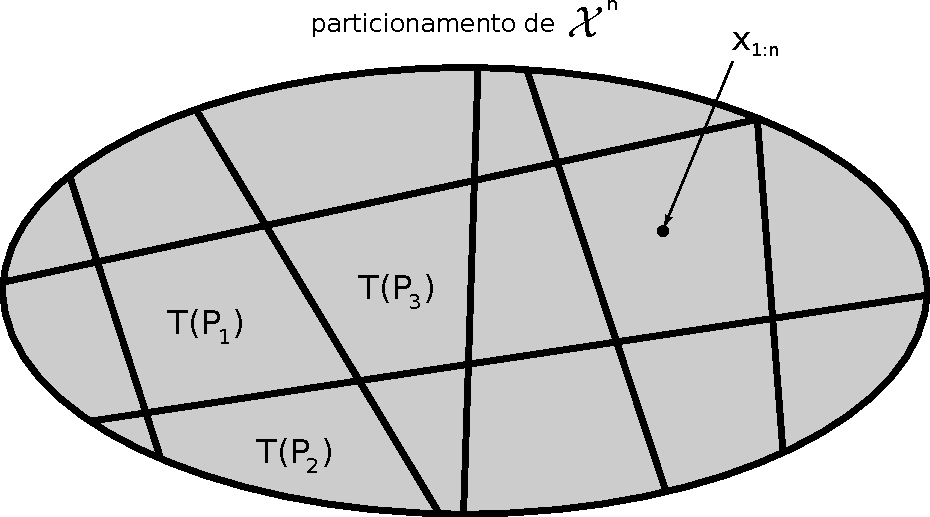
\includegraphics[width=0.8\textwidth]{images/particao-Xn2.pdf}
  %\caption{.}
  \label{fig:particao-Xn}
  \end{figure}
\end{frame}


\subsection{Limite no Número de Tipos}
\begin{frame}[allowframebreaks]
  \frametitle{Limite no Número de Tipos}
  \begin{theorem}[Limite no número de tipos]
  O número de tipos para sequências de comprimento $n$ em um alfabeto $\mathcal{X}$ é limitado por
	\begin{equation}
	\label{eq:number-of-types-bound}
	\vert \mathcal{P}_n \vert \leq (n+1)^{\vert \mathcal{X} \vert} .
	\end{equation}
  \end{theorem}
  \begin{proof}
	\begin{itemize}
	\item Note que o numerador de cada entrada em um tipo pode assumir $(n+1)$ valores distintos (de $0$ a $n$).
	\item Existem $\vert \mathcal{X} \vert$ entradas em um tipo, e portanto a mesma quantidade de numeradores.
	\item Os valores dos numeradores interagem entre si (a soma de todos deve ser igual a $n$), mas podemos
		achar um limite superior desconsiderando esta interação. 
	\item Logo, 
	        \vspace{-2ex}
		\begin{equation}
		\vert \mathcal{P}_n \vert \leq \underbrace{(n+1)\times(n+1)\times\ldots\times(n+1)}_{\vert \mathcal{X} \vert \text{ vezes}} = (n+1)^{\vert \mathcal{X} \vert} .
		\end{equation}
	\end{itemize}
  \end{proof}

  \framebreak
  \begin{itemize}
  \item Importante notar que existe no máximo um número polinomial em $n$ de tipos de sequencias de comprimento $n$.
  \item Além disso, $\exists$ um número exponencial de sequências com comprimento $n$, $\vert \mathcal{X} \vert^n$, e 
	um número (no máximo) polinomial de tipos.
  \item Eventualmente, um dos tipos (um dos blocos na partição) conterá todas as sequências.
  \end{itemize}
\end{frame}
\note{
Note que calcular Equação \ref{eq:number-of-types} é muito mais complicado do que calcular \ref{eq:number-of-types-bound}, e como visto
o limite será suficiente para o que queremos mostrar.
}



\subsection{Probabilidade Depende do Tipo}
\begin{frame}[allowframebreaks]
  \frametitle{Probabilidade Depende do Tipo}
  \begin{theorem}[Probabilidade Depende do Tipo]
	Seja $X_1, X_2, \ldots, X_n$ i.i.d. $\sim Q(x)$, com $Q$ arbitrário, e extensão 
	$Q^n(x_{1:n}) = \prod_i Q(x_i)$, a probabilidade da sequencia depende apenas do tipo, ou seja,
	a probabilidade é `independente' da sequencia, dado o tipo e $Q$, isto é,
	\begin{equation}
	Q^n(x_{1:n}) = 2^{-n[ H(P_{x_{1:n}}) + D(P_{x_{1:n}}||Q) ]}
	\end{equation}
  \end{theorem}
  \begin{itemize}
  \item Probabilidade não depende da sequencia, dado o tipo.
  \item Estatística Suficiente.
  \item Todas as sequencias do mesmo tipo possuem a mesma probabilidade.
  \end{itemize}

  \framebreak
  \begin{proof}
  \vspace{-0.2cm}
  \begin{eqnarray}
  Q^n(x_{1:n}) &=& \prod_{i=1}^{n} Q(x_i) = \prod_{a \in \mathcal{X}} Q(a)^{n(a \mid x_{1:n})} \nonumber \\
	&=& \prod_{a \in \mathcal{X}} Q(a)^{n P_{x_{1:n}}(a) } = \prod_{a \in \mathcal{X}} 2^{ \left\{ n P_{x_{1:n}}(a) \log Q(a) \right\} } \nonumber \\
	&=& \prod_{a \in \mathcal{X}} 2^{ n \left\{  P_{x_{1:n}}(a) \log Q(a) \KeepStyleUnderBrace{ -P_{x_{1:n}}(a) \log P_{x_{1:n}}(a) + P_{x_{1:n}}(a) \log P_{x_{1:n}}(a) }_{=0} \right\} } \nonumber \\
	&=& 2^{n \sum_{a \in \mathcal{X}}  \left( -P_{x_{1:n}}(a) \log \frac{P_{x_{1:n}}(a)}{Q(a)} + P_{x_{1:n}}(a) \log P_{x_{1:n}}(a) \right)  } \nonumber \\
	&=& 2^{-n \left( D(P_{x_{1:n}} \mid \mid Q) + H( P_{x_{1:n}} ) \right) }
  \end{eqnarray}
  \end{proof}

  \framebreak

  \begin{itemize}
  \item (corolário) Se $Q$ é uma distribuição racional (i.e., um tipo possível) e se $x_{1:n} \in T(Q)$, então
	\begin{equation}
	Q^n(x_{1:n}) = 2^{-n H(Q)} .
	\end{equation}
  \item O que ocorre se $Q$ for irracional? Podemos fazer $D(P_{x_{1:n}} \mid \mid Q)$  tão pequeno quando desejável,
	fazendo $n$ grande suficiente.
  \end{itemize}
\end{frame}


\subsection{Tamanho da Classe de Tipo}
\begin{frame}[allowframebreaks]
  \frametitle{Classe de Tipo com maior probabilidade}
  \begin{itemize}
  \item Qual classe de tipo possui maior probabilidade quando a distribuição geradora das sequências é
	$P \in \mathcal{P}_n$?
  \item Considerando a Prop. da Eq. Ass., as sequências típicas são aquelas mais próximas da real distribuição,
	e elas possuem `toda' probabilidade.
  \item Vamos supor então que $T(P)$ possui a maior probabilidade sob a distribuição $P$.
  \end{itemize}

  \begin{lemma}
  Para $P \in \mathcal{P}_n$, teremos que $T(P)$ possui a maior probabilidade. Isto é
	\begin{equation}
	P^n(T(P)) \geq P^n(T(\hat{P})) , \ \forall \hat{P} \in \mathcal{P}_n .
	\end{equation}
  \end{lemma}
  Nota: Sejam $m$ e $n$ inteiros não negativos, então $\frac{m!}{n!} \geq n^{m-n}$. 
	Se $m>n$, então $\frac{m!}{n!} = m(m-1) \ldots (n+1) \geq n^{m-n}$.
	Se $m<n$, então $\frac{m!}{n!} = \frac{1}{n(n-1)\ldots(m+1)} \geq \frac{1}{n^{n-m}}$.
	Se $m=n$, $\frac{m!}{n!} = 1 = n^0$.

  \framebreak

  \begin{proof}
  \vspace{-0.2cm}
  \begin{eqnarray}
  \frac{P^n(T(P))}{P^n(T(\hat{P}))} &=& \frac{\vert T(P) \vert \prod_{a \in \mathcal{X}} P(a)^{nP(a)} }{ \vert T(\hat{P}) \vert \prod_{a \in \mathcal{X}} P(a)^{n\hat{P}(a)}  } \nonumber \\
	&=& \frac{ { n \choose nP(a_1) \ nP(a_2) \ \ldots \ nP(a_D) } \prod_{a \in \mathcal{X}} P(a)^{nP(a)} }{ { n \choose n\hat{P}(a_1) \ n\hat{P}(a_2) \ \ldots \ n\hat{P}(a_D) } \prod_{a \in \mathcal{X}} P(a)^{n\hat{P}(a)}  } \nonumber \\
	&=& \prod_{a \in \mathcal{X}} \frac{ [n\hat{P}(a)]! }{[nP(a)]!} P(a)^{n(P(a)-\hat{P}(a))} \nonumber \\
	&\geq& \prod_{a \in \mathcal{X}} (nP(a))^{n(\hat{P}(a)-P(a))} P(a)^{n(P(a)-\hat{P}(a))} \nonumber \\
	&=& \prod_{a \in \mathcal{X}} n^{n(\hat{P}(a)-P(a))}  
  \end{eqnarray}
  \proofbreak
  \vspace{-2ex}
  \begin{eqnarray}
  \frac{P^n(T(P))}{P^n(T(\hat{P}))} &=& \ldots \nonumber \\
	&\geq& \prod_{a \in \mathcal{X}} n^{n(\hat{P}(a)-P(a))} \nonumber \\
	&=& n^{n\left[ \sum_{a \in \mathcal{X}} \hat{P}(a) - \sum_{a \in \mathcal{X}} P(a) \right]} \nonumber \\
	&=& n^{n(1-1)} = 1
  \end{eqnarray}
  logo, $P^n(T(P)) \geq P^n(T(\hat{P}))$.
  \end{proof}
\end{frame}



\begin{frame}[allowframebreaks]
  \frametitle{Tamanho da Classe de Tipo}
  Podemos expressar o tamanho de uma classe de tipo utilizando os coeficientes multinomiais,
  i.e., o número de maneiras de escolher símbolos distintos do alfabeto para cada elemento
  da sequencia $x_{1:n}$. 

  Para $P \in \mathcal{P}_n$, temos
  \begin{equation}
  \vert T(P) \vert = { n \choose nP(a_1) \ nP(a_2) \ \ldots \ nP(a_n) }
  \end{equation}

  Entretanto, isto é difícil calcular. Queremos encontrar limites que sejam mais facilmente manipulados matematicamente.

  \framebreak

  \begin{theorem}[Limites no tamanho da Classe de Tipo]
  Dado um tipo $P \in \mathcal{P}_n$, temos
	\begin{equation}
	\frac{1}{(n+1)^{\vert \mathcal{X} \vert}} 2^{nH(P)} \leq \vert T(P) \vert \leq 2^{nH(P)}
	\end{equation}
  \end{theorem}
 
  \begin{proof}[limite superior]
  \begin{eqnarray}
  1 &\geq& P^{n} (T(P)) = \sum_{x_{1:n} \in T(P)} P^{n} (x_{1:n}) = \sum_{x_{1:n} \in T(P)} 2^{-nH(P)} \nonumber \\
    &=& \vert T(P) \vert 2^{-nH(P)}
  \end{eqnarray}
  \end{proof}

  \framebreak

  \begin{proof}[limite inferior]
  \begin{eqnarray}
  1 &=& \sum_{Q \in \mathcal{P}_n} P^n (T(Q)) \leq \sum_{Q \in \mathcal{P}_n} \max_{R \in \mathcal{P}_n} P^n (T(R)) \nonumber \\
	 && \text{fazendo } P = \argmax_{R \in \mathcal{P}_n} P^n (T(R)) \text{ teremos } \nonumber \\
	&=& \sum_{Q \in \mathcal{P}_n} P^n (T(P)) \leq (n+1)^{\vert \mathcal{X} \vert} P^n (T(P)) \nonumber \\
	&=& (n+1)^{\vert \mathcal{X} \vert} \sum_{x_{1:n} \in T(P)} P^n (x_{1:n}) \nonumber \\
	&=& (n+1)^{\vert \mathcal{X} \vert} \sum_{x_{1:n} \in T(P)} 2^{-nH(P)} 
  \end{eqnarray} 
  \proofbreak
  \begin{eqnarray}
  1 &=& \ldots \nonumber \\
	&\leq& (n+1)^{\vert \mathcal{X} \vert} \sum_{x_{1:n} \in T(P)} 2^{-nH(P)} \nonumber \\
	&=& (n+1)^{\vert \mathcal{X} \vert} \vert T(P) \vert 2^{-nH(P)}
  \end{eqnarray}
 
  fornecendo assim o resultado
  \begin{equation}
  \vert T(P) \vert \geq \frac{1}{(n+1)^{\vert \mathcal{X} \vert}} 2^{nH(P)}
  \end{equation}
  \end{proof}

\end{frame}

\subsection{Exemplo Binário}
\begin{frame}[allowframebreaks]
  \frametitle{Limites Combinatórios}
  \begin{itemize}
  \item Para o caso binário, $\mathcal{X} = \{0,1\}$, temos os seguintes limites
	\begin{equation}
	\frac{1}{(n+1)^2} 2^{nH(\frac{k}{n})} \leq {n \choose k} \leq 2^{nH(\frac{k}{n})}
	\end{equation}
  \item O limite inferior pode ser ainda mais restrito neste caso 
	\begin{equation}
        \frac{1}{(n+1)} 2^{nH(\frac{k}{n})} \leq {n \choose k} \leq 2^{nH(\frac{k}{n})}
        \end{equation}
  \end{itemize}
\end{frame}

\subsection{Probabilidade da classe de tipo}
\begin{frame}[allowframebreaks]
  \frametitle{Probabilidade da classe de tipo}
   \begin{theorem}
   Para qualquer $P \in \mathcal{P}_n$ e qualquer distribuição $Q$, a probabilidade da classe de tipo
   $T(P)$ sob $Q^n$ é tal que $Q^n(T(P)) \circeq 2^{-n D(P \mid \mid Q)}$. Especificamente, temos os limites
   \begin{equation}
   \frac{1}{(n+1)^{\vert \mathcal{X} \vert}} 2^{-n D(P \mid \mid Q)} \leq Q^n(T(P)) \leq 2^{-nD(P \mid \mid Q)}
   \end{equation}
   \end{theorem}
   obs.: qualquer tipo menos próximo do tipo mais próximo de $Q$ irá ter probabilidade exponencialmente decrescente com $n$, 
   decrescendo mais rapidamente que o tipo mais provável.
   \framebreak
   \begin{proof}
   \begin{eqnarray}
   Q^n(T(P)) &=& \sum_{x_{1:n} \in T(P)} Q^n(x_{1:n}) = \sum_{x_{1:n} \in T(P)} 2^{-n (D(P \mid \mid Q) + H(P))} \nonumber \\
	&=& \vert T(P) \vert 2^{-n (D(P \mid \mid Q) + H(P))}
   \end{eqnarray}
   para completar a demonstração, devemos utilizar 
        \begin{equation}
        \frac{1}{(n+1)^{\vert \mathcal{X} \vert}} 2^{nH(P)} \leq \vert T(P) \vert \leq 2^{nH(P)}
        \end{equation}
   \end{proof}

   \framebreak

   \begin{itemize}
   \item Quais tipos terão maior probabilidade?
   \item Claramente aqueles mais próximos da real distribuição.
   \item A propriedade $Q^n(T(P)) \circeq 2^{-n D(P \mid \mid Q)}$ diz que aqueles
	mais distantes terão probabilidade exponencialmente menor do que os demais, quando $n \rightarrow \infty$.
   \end{itemize}

\end{frame}


\subsection{Sumário}
\begin{frame}[allowframebreaks]
  \frametitle{Sumário}
   \begin{itemize}
   \item Número de tipos de sequências com comprimento $n$
	\begin{equation}
	\vert \mathcal{P}_n \vert \leq (n+1)^{\vert \mathcal{X} \vert}
	\end{equation}
   \item A probabilidade da sequência ($p(x_{1:n})$) depende apenas do tipo 
	\begin{equation}
	Q^n(x_{1:n}) = 2^{-n [H(P_{x_{1:n}}) + D(P_{x_{1:n}} \mid \mid Q)]}
	\end{equation}
   \item Tamanho da Classe de Tipo
	\begin{equation}
	\vert T(P) \vert \circeq 2^{nH(P)}
        \end{equation}
   \item Probabilidade da classe de tipo
	\begin{equation}
	Q^n(T(P)) \circeq 2^{-nD(P \mid\mid Q)}
	\end{equation}
   \end{itemize}
\end{frame}



\subsection{Conjunto Típico}
\begin{frame}[allowframebreaks]
  \frametitle{Conjunto Típico}
  \begin{itemize}
  \item Os tipos $P$ mais próximos da real distribuição $Q$ terão maior probabilidade.
  \item Aqueles mais distantes de $Q$ terão probabilidade exponencialmente menor do que os demais.
  \end{itemize}

   \begin{definition}[conjunto típico de sequências]
   Seja $X_1, X_2, \ldots, X_n$ i.i.d. $\forall i$, $X_i \sim Q(x)$. Então o conjunto típico é definido como
        \begin{equation}
        T^{\epsilon}_{Q} = \{ x_{1:n} : D(P_{x_{1:n}} \mid \mid Q) \leq \epsilon \}
        \end{equation}
   \end{definition}

   \framebreak

  \begin{theorem}[probabilidade do conjunto típico]
  Sejam $X_1, X_2, \ldots, X_n$ i.i.d. $\forall i$, $X_i \sim Q(x)$. A probabilidade do complemento
  do conjunto típico $\overline{T}^{\epsilon}_Q$ é dada por
	\begin{equation}
	Q(\overline{T}^{\epsilon}_Q) = Q( \{ x_{1:n} : D(P_{x_{1:n}} \mid\mid Q) > \epsilon  \} ) \leq 2^{-n (\epsilon - \vert \mathcal{X} \vert \frac{\log (n+1)}{n})}
	\end{equation}
  desta forma
	\begin{equation}
	D(P_{x_{1:n}} \mid\mid Q) \xrightarrow{p} 0 \text{ quando } n \rightarrow \infty
	\end{equation}
  (converge em probabilidade para zero quando $n$ é grande suficiente)
  \end{theorem}
  \begin{itemize}
  \item Os tipos que divergem (KL) mais do que $\epsilon$ da distribuição subjacente $Q$ terão probabilidade decrescente. 
  \item Para $n$ grande, o conjunto típico acaba sendo a única coisa que ocorre com uma probabilidade não evanescente.
  \end{itemize} 

  \framebreak

  \begin{proof}
  \begin{eqnarray}
  1 - Q^{n}(T^{\epsilon}_Q) &=& Q(\overline{T}^{\epsilon}_Q) = \sum_{P \in \mathcal{P}_n : D(P \mid\mid Q) > \epsilon} Q^n (T(P)) \nonumber \\
	&\leq& \sum_{P \in \mathcal{P}_n : D(P \mid\mid Q) > \epsilon} 2^{-n D(P\mid\mid Q)} \nonumber \\
	&\leq& \sum_{P \in \mathcal{P}_n : D(P \mid\mid Q) > \epsilon} 2^{-n \epsilon} \nonumber \\
	&\leq& (n+1)^{\vert \mathcal{X}  \vert} 2^{-n \epsilon} = 2^{-n \left( \epsilon - \vert \mathcal{X} \vert \frac{\log (n+1)}{n}  \right)}
  \end{eqnarray}
  então a probabilidade vai para zero quando $n \rightarrow \infty$, e desta forma a probabilidade do conjunto típico vai para $1$ quando $n \rightarrow \infty$.
  \end{proof}

  \framebreak

  \begin{itemize}
  \item Com qual frequência um evento atípico ocorre?
  \item Como $p(\overline{T}^{\epsilon}_Q) \leq 2^{-n \left( \epsilon - \vert \mathcal{X} \vert \frac{\log (n+1)}{n}  \right)}$, uma 
	sequencia em $n$ exponencial decrescente. Esta será, desta forma, somável.
	\begin{equation}
	\infty > \sum_{n=1}^{\infty} p(D(P_{x_{1:n}} \mid\mid Q) > \epsilon) = E_Q \left[ \sum_{n=1}^{\infty} \mathbf{1}_{\{ D(P_{X_{1:n}} \mid\mid Q) > \epsilon \}}  \right]
	\end{equation}
  \item O número esperado de vezes que o evento $D(P_{X_{1:n}} \mid\mid Q) > \epsilon$ ocorre é finito, dentro de um conjunto infinito de possíveis ocorrências.
  \end{itemize}
\end{frame}




\subsection{Codificação Universal de Fonte}
\begin{frame}[allowframebreaks]
  \frametitle{Codificação Universal de Fonte}
  \begin{itemize}
  \item Dizemos que uma codificação de fonte é universal quando ela não depende de $p(x)$.
  \item Codificação não universal: Se conhecemos $p(x)$, podemos propor um código para comprimir a fonte caracterizada por $p(x)$.
	Exemplo: Código de Huffman.
  \item É possível criar um código universal (não dependente de $p(x)$) que atinja o limite da entropia? taxa $R > H(Q)$ (em bits por símbolo)
  \item O que ocorre se $R < H(Q)$?
  \item Ideia similar àquela do conjunto típico $A_{\epsilon}^{(n)}$. Vamos codificar apenas aquilo que de fato ocorre.
	Precisaremos de no máximo $\vert A_{\epsilon}^{(n)} \vert$ palavras que podem ser indexadas com $nH$ bits.
  \item Vamos formalizar o teorema de Shannon utilizando o método de tipo.
  \end{itemize}

  \framebreak

  \begin{itemize}
  \item Existem no máximo $2^{nH(P)}$ sequências do tipo $P$. Podermos utilizar $nH(P)$ bits para representar tais sequencias.
  \item Se $R > H(P)$, podemos utilizar $nR$ bits para representar estas sequências.
  \item Quando $n$ cresce, apenas os tipos $P$ `próximos' de $Q$ irão ocorrer.
  \item Existe um número exponencial (em $n$) de sequências e um número polinomial (em $n$) de tipos.
  \item Eventualmente, um tipo terá `toda' a probabilidade.
  \end{itemize}

  \framebreak
 
  \begin{figure}[h!]
  \centering
  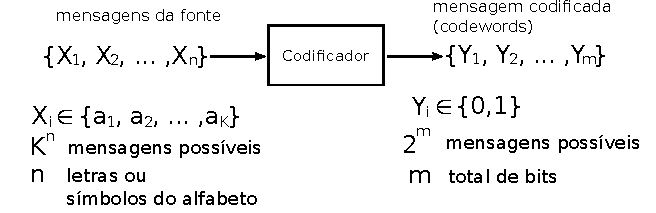
\includegraphics[width=0.9\textwidth]{images/blockcoding.pdf}
  %\caption{.}
  \label{fig:blockcoding-types}
  \end{figure}

\end{frame}


\begin{frame}[allowframebreaks]
  \frametitle{Códigos $(M,n)$}
  \begin{itemize}
  \item código de blocos com taxa fixa $R$
  \item Existem $M$ palavras. $M$ é o número de possíveis mensagens.
  \item $n$ símbolos são codificados conjuntamente a cada instante.
  \item O codificador faz o mapeamento de \textit{strings} de tamanho $n$ produzidas pela fonte em \textit{strings} de $m$ bits.
    \begin{figure}[h!]
    \centering
    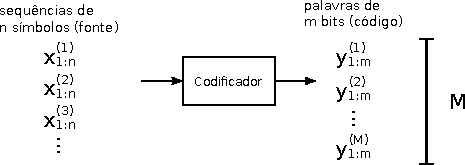
\includegraphics[width=0.9\textwidth]{images/Mncodes2.pdf}
    %\caption{.}
    \label{fig:Mncodes}
    \end{figure}
  \item A taxa $R$ depende de $M$ e $n$.
	\begin{equation}
	R = \frac{\log M}{n} = \frac{\log (\text{n. de palavras}) }{\text{n. de símbols}}
	\end{equation}
  \end{itemize}

  \framebreak

  \begin{definition}[código de bloco com taxa fixa $R$]
  Seja $X_1, X_2, \ldots, X_n \sim Q$, i.i.d. mas $Q$ desconhecido. A função do codificador
  e decodificador são definidas a seguir:
	\begin{equation}
	\text{codificador: } f_n : \mathcal{X}^n \rightarrow \{1,2,\ldots,2^{nR}\}
	\end{equation}
	\begin{equation}
        \text{decodificador: } \phi_n : \{1,2,\ldots,2^{nR}\} \rightarrow \mathcal{X}^n
	\end{equation}
  e a probabilidade de erro
	\begin{equation}
	P_e^{(n)} = Q^n (\{ x_{1:n} : \phi (f_n (x_{1:n})) \neq x_{1:n} \})
        \end{equation}	
  \end{definition}

  \framebreak

  \begin{definition}[código de bloco universal de taxa $R$]
  Um código de bloco de taxa $R$ para um fonte é dito universal se a função $f_n$ e $\phi_n$
  não depender da distribuição $Q$ e se 
	\begin{equation}
	P_e^{(n)} \rightarrow 0 \text{ quando } n \rightarrow \infty \text{ sempre que } H(Q) < R
        \end{equation}
  \end{definition}
  \begin{itemize} 
  \item Se $R > H(Q)$, então existe uma sequência (em $n$) de códigos com erro evanescente.
  \item Por outro lado, se $R < H(Q)$ a probabilidade de erro vai pra 1.
  \end{itemize}
\end{frame}


\subsection{Teorema da Codificação de Shannon}

\begin{frame}[allowframebreaks]
  \frametitle{Simplex Probabilístico}

  \begin{definition}[Simplex Probabilístico]
  O Simplex Probabilístico em $\RealNumber^m$ é o conjunto de pontos
  $x_{1:m} = (x_1, x_2, \ldots, x_m) \in \RealNumber^m$ tal que $x_i \geq 0$, $\sum_{i=1}^{m} x_i = 1$.
  \end{definition}
  \framebreak 
  \begin{example}[$m=2$]
  O Simplex probabilístico será o conjunto de pontos
  \begin{equation}
  \{ (x_1, x_2)  :  x_1 \geq 0 , x_2 \geq 0 , x_1 + x_2 = 1 \}
  \end{equation}
    \begin{figure}[h!]
    \centering
    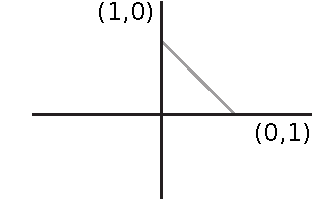
\includegraphics[width=0.4\textwidth]{images/prob-simplex-2.pdf}
    %\caption{.}
    \label{fig:prob-simplex-2}
    \end{figure}

  \end{example}
  \framebreak
  \begin{example}[$m=3$]
  O Simplex probabilístico será o conjunto de pontos
  \begin{equation}
  \{ (x_1, x_2, x_3)  :  x_1 \geq 0 , x_2 \geq 0 , x_3 \geq 0 , x_1 + x_2 + x_3 = 1 \}
  \end{equation}

    \begin{figure}[h!]
    \centering
    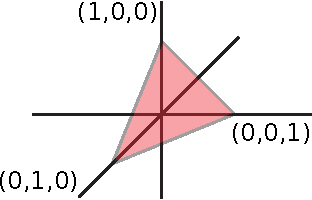
\includegraphics[width=0.4\textwidth]{images/prob-simplex-3.pdf}
    %\caption{.}
    \label{fig:prob-simplex-3}
    \end{figure}

  \end{example}

  \framebreak
  Os tipos em para $\vert \mathcal{X} \vert = m$ podem ser representados em um Simplex Probabilístico em $\RealNumber^m$.
  \begin{example}[$\vert \mathcal{X} \vert = 3$]
    \begin{figure}[h!]
    \centering
    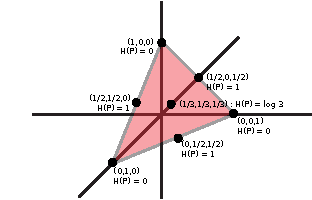
\includegraphics[width=0.5\textwidth]{images/prob-simplex-types3.pdf}
    %\caption{.}
    \label{fig:prob-simplex-3}
    \end{figure}
  \end{example}

\end{frame}


\begin{frame}[allowframebreaks]
  \frametitle{Teorema da Codificação de Shannon}
  \begin{theorem}[Teorema da Codificação de Shannon]
  $\exists$ uma sequencia $(2^{nR},n)$ de códigos universais tais que $P_e^{(n)} \rightarrow 0$ para toda
  distribuição $Q$ tal que $H(Q) < R$.
  \end{theorem}

  \framebreak 

  \begin{proof}
  \begin{itemize}
  \item Fixe $R > H(Q)$.
  \item Defina uma taxa para $n$ que é fixada a um fator polinomial.
	\begin{equation}
	R_n \triangleq R - \vert \mathcal{X} \vert \frac{\log (n+1)}{n} < R
	\end{equation}
  \item Defina um conjunto de sequências que possuem entropia de tipo menor do que esta taxa.
	\begin{eqnarray}
	A_n &\triangleq& \{ x_{1:n} \in \mathcal{X}^n : H(P_{x_{1:n}}) \leq R_n \} \nonumber \\
		&=& \left\{  \bigcup_{P \in \mathcal{P}_n} T(P) : H(P) \leq R_n \right\}
	\end{eqnarray}
  \end{itemize}
 
  \proofbreak

  \begin{itemize}
  \item Temos então
  \begin{eqnarray}
	\vert A_n \vert &=& \sum_{P \in \mathcal{P}_n : H(P) \leq R_n} \vert T(P) \vert \leq \sum_{P \in \mathcal{P}_n : H(P) \leq R_n} 2^{nH(P)} \nonumber \\
			&\leq& \sum_{P \in \mathcal{P}_n : H(P) \leq R_n} 2^{nR_n} \leq (n+1)^{\vert \mathcal{X} \vert} 2^{nR_n} \nonumber \\
			&=& 2^{n \left( R_n + \vert \mathcal{X} \vert \frac{\log (n+1)}{n} \right)} = 2^{nR} .
  \end{eqnarray}
  \item Como $\vert A_n \vert \leq 2^{nR}$, podemos indexar $A_n$ com $nR$ bits.
  \end{itemize}  

  \proofbreak

  O codificador será dada por
  \begin{equation}
  f_n (x_{1:n}) = \begin{cases} 
		\text{índice de } x_{1:n} \text{ em } A_n ,	\quad \text{ se } x_{1:n} \in A_n \\
		0					,	\quad \text{ caso contrário }.
		\end{cases}
  \end{equation}

  \begin{itemize}
  \item O codificador associará um índice a $x_{1:n}$ se $H(P_{x_{1:n}}) \leq  R_n$ (ou seja, $x_{1:n} \in A_n$); 
  e não associará valor se $H(P_{x_{1:n}}) >  R_n$ (ou seja, $x_{1:n} \notin A_n$).
  \item Note que $f_n(\cdot)$ não depende da distribuição da fonte, apenas do ordenamento e de $\RealNumber^m$.
  \item Um erro ocorrerá se $x_{1:n} \notin A_n$.
  \end{itemize}
  
  \proofbreak
  Os tipos podem ser representados por pontos em um Simplex Probabilístico.
    \begin{figure}[h!]
    \centering
    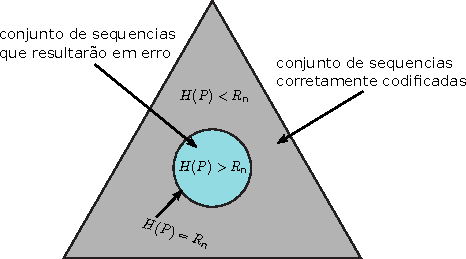
\includegraphics[width=0.5\textwidth]{images/type-simplex.pdf}
    %\caption{.}
    \label{fig:type-simplex}
    \end{figure}

  \proofbreak

  Um erro ocorre quando a sequência não está em $A_n$. Desta forma,
  \begin{eqnarray}
  P_e^{(n)} &=& 1 - Q^n(A_n) = \sum_{P: H(P) > R_n} Q^n (T(P)) \nonumber \\
	&\leq& \sum_{P: H(P) > R_n} \max_{P: H(P) > R_n} Q^n (T(P)) \nonumber \\
	&\leq& (n+1)^{\vert \mathcal{X} \vert} \max_{P: H(P) > R_n} Q^n (T(P)) \nonumber \\
	&\leq& (n+1)^{\vert \mathcal{X} \vert} \max_{P: H(P) > R_n} 2^{-n  D(P \mid\mid Q)} \nonumber \\
	&=& (n+1)^{\vert \mathcal{X} \vert} 2^{-n [\min_{P: H(P) > R_n} D(P \mid\mid Q)]}
  \end{eqnarray}
  %onde utilizamos que $Q^n(T(P)) \leq 2^{-n D(P\mid \mid Q)}$.


  \proofbreak

  \begin{itemize}
  \item Temos que $R_n$ forma uma sequência crescente com $n$, tal que $R_n < R$ para todo $n$.
  \item Por hipótese, $H(Q) < R$.
  \item Eventualmente, para algum $n_0$, teremos que $\forall n > n_0$, $R_n > H(Q)$.
  \item Na equação anterior, escolhemos $P: H(P) > R_n$.

    \begin{figure}[h!]
    \centering
    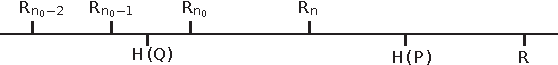
\includegraphics[width=0.9\textwidth]{images/Rn-seq.pdf}
    %\caption{.}
    \label{fig:Rn-seq}
    \end{figure}

  \item Teremos então: $H(P) > R_n > H(Q)$, o que implica em $P \neq Q$.
  \item Desta forma, teremos $D(P \mid\mid Q) > 0$ para $P$ escolhido.
  \end{itemize}


  \proofbreak

  \begin{itemize}
  \item Teremos assim
	\begin{equation}
	P_e^{(n)} \leq \underbrace{(n+1)^{\vert \mathcal{X} \vert}}_{\text{polinomial em } n} \underbrace{ 2^{-n [\min_{P: H(P) > R_n} D(P \mid\mid Q)]} }_{\text{exp. decrescente qnd } n \rightarrow \infty}
	\end{equation}
  \item Logo, $P_e^{(n)} \rightarrow 0$ quando $n \rightarrow \infty$.
  \end{itemize}


  \end{proof}

  \begin{itemize}
  \item Por outro lado, se $R < H(Q)$ teremos $P_e^{(n)} \rightarrow 1$.
  \item Entropia é o limite de compressão.
  \end{itemize}

\end{frame}



% processos estocásticos
\section{Processos Estocásticos}

\begin{frame}[allowframebreaks]
  \frametitle{Processo Estocástico}
  \begin{itemize}
  \item Falamos de variáveis aleatórias i.i.d. $X_1,X_2, \ldots$. Neste contexto, cada uma delas possui a mesma entropia associada.
  \item O que ocorre quando as v.a.s. não são mais independentes? Como podemos lidar com a entropia do processo, neste caso?
  \end{itemize}

  \begin{definition}[Processo Estocástico Estacionário (sentido-estrito)]
  Uma sequência de v.a.s. $X_1, X_2, \ldots, X_n$ é governada por uma distribuição probabilística é dita
  estacionária em sentido estrito se
	\begin{equation}
	p(X_{1:n} = x_{1:n}) = p(X_{1+l:n+l} = x_{1:n})
	\end{equation}  
  para todo $l$, todo $n$ e todo $x_{1:n} \in \mathcal{X}^n$.
  \end{definition}
\end{frame}

\begin{frame}[allowframebreaks]
  \frametitle{Processo de Markov}

  \begin{definition}[Processo de Markov de primeira ordem]
  Um processo estocástico é um processo de Markov de primeira ordem se
	\begin{equation}
	p(X_{n+1} = x_{n+1} \mid X_{1:n} = x_{1:n}) = p(X_{n+1} = x_{n+1} \mid X_n = x_n)
	\end{equation}
  \end{definition}
  Neste caso, isto significa que $p(x_{1:n}) = p(x_1)p(x_2 \mid x_1) \ldots p(x_n \mid x_{n-1})$.

  Dado o presente, o futuro e o passado são independentes.


  \begin{definition}[Processo de Markov de ordem $m$]
  Um processo estocástico é um processo de Markov de ordem $m$ se
        \begin{eqnarray}
        p(X_{n+1} = x_{n+1} \mid X_{1:n} = x_{1:n}) = \nonumber \\
	p(X_{n+1} = x_{n+1} \mid X_n = x_n, X_{n-1} = x_{n-1}, \ldots , X_{n-m} = x_{n-m})
        \end{eqnarray}
  \end{definition}
  Neste caso, isto significa que $p(x_{1:n}) = p(x_{m+1} \mid x_{m}, x_{m-1}, \ldots, p(x_1)) \ldots p(x_{n-1} \mid x_{n-2}, x_{n-3}, \ldots, x_{n-m-1})  p(x_n \mid x_{n-1}, x_{n-2}, \ldots, x_{n-m})$.

        \begin{figure}[h!]
        \centering
        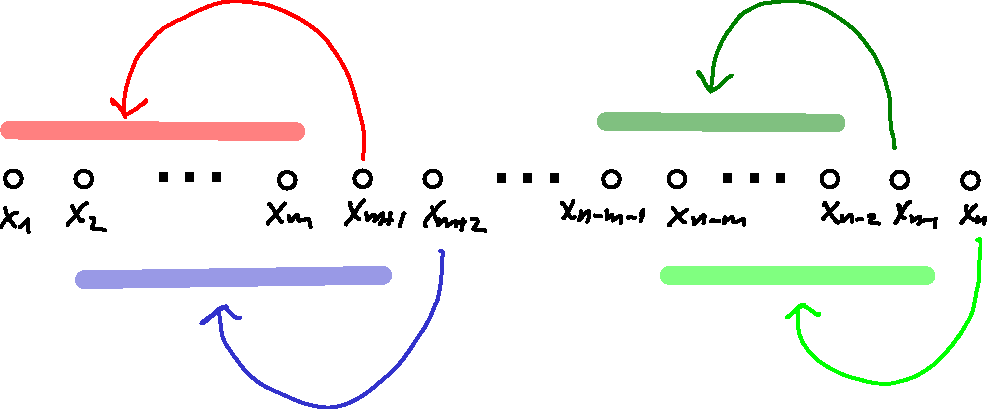
\includegraphics[width=0.8\textwidth]{images/markov-morder.pdf}
        \label{fig:markov-morder}
        \end{figure}

   \framebreak

   \begin{definition}[Homogêneo]
   Uma cadeia de Markov é invariante no tempo (também chamada de homogênea) se $p(x_{n+1} \mid x_n)$ não
   depender do tempo, i.e., se
	\begin{equation}
	p(X_{n+1} = b \mid X_{n} = a) = p(X_2 = b \mid X_1 = a) \quad \forall a,b,n
	\end{equation}   
   \end{definition}
   Neste caso, a cadeia de Markov pode ser descrita por uma matriz de transição fixa $P = [p_{ij}]_{ij}$
   em que $p_{ij} = p(X_{n+1} = j \mid X_{n} = i)$. Podemos representar esta cadeia de Markov como um grafo 
   com setas entre estados cuja probabilidade de transição não é nula.

   \framebreak

   \begin{columns}
   \begin{column}{0.5\textwidth}
	\begin{equation}
	P = \begin{bmatrix}
		0 & p(2 \mid 1) & 0 & p(4 \mid 1) \\
		0 & p(2 \mid 2) & p(3 \mid 2) & 0 \\
		0 & 0 & 0 & p(4 \mid 3) \\
		0 & 0 & 0 & p(4 \mid 4) \\
		\end{bmatrix}
	\end{equation}
   \end{column}
   \begin{column}{0.5\textwidth}
	\begin{figure}[h!]
	\centering
	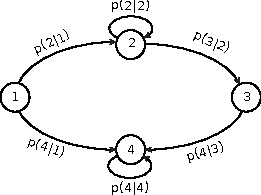
\includegraphics[width=0.6\textwidth]{images/markov-example.pdf}
	\label{fig:markov-example}
	\end{figure}
   \end{column}
   \end{columns}
 
   \begin{itemize}
   \item A probabilidade de um estado no instante $n+1$, dada em função dos possíveis estados no instante $n$ e da probabilidade de transição:
	\begin{equation}
	p(x_{n+1}) = \sum_{x_n} p(x_n) p_{x_n  x_{n+1}}
	\end{equation}
   \item uma cadeia de Markov de primeira ordem é estacionária se $p(x_{n+1}) = p(x_n)$.
   \end{itemize}

   \framebreak

   \begin{definition}[Irredutível]
   Uma cadeia de Markov é irredutível se $p_{ij}(n) > 0$ para todo $i,j$ e para algum $n$ onde
   $p_{ij}(n) = p(X_{n+1} = j \mid X_{n} = i)$.
   \end{definition}
   Ou seja, qualquer estado é acessível de qualquer outro estado (ao menos em algum instante $n$),
   com probabilidade não nula.

   \framebreak

   \begin{definition}[Período]
   Uma cadeia de Markov é periódica se $d(i) > 1$ com
	\begin{equation}
	d(i) = \gcd \{ n : p_{ii}(n) > 0 \}
	\end{equation}
   $d(i)$ é o período do $i$-ésimo estado.
   \end{definition}
   Note que temos o máximo divisor comum do número de épocas para o qual um retorno ao mesmo estado é possível.


   No caso de uma cadeia de Markov homogênea (invariante no tempo), se houver algum $p_{ii} > 0$, 
   o período será $1$ época.

   \framebreak

   \begin{example}
     \begin{columns}
     \begin{column}{0.5\textwidth}
	\begin{equation}
	P = \begin{pmatrix} 1 - \alpha & \alpha \\ \beta & 1 - \beta \end{pmatrix}
	\end{equation}
     \end{column}
     \begin{column}{0.5\textwidth}
        \begin{figure}[h!]
        \centering
        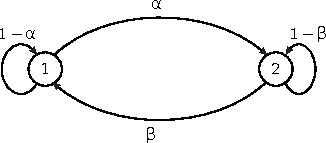
\includegraphics[width=0.6\textwidth]{images/markov-example2.pdf}
        \label{fig:markov-example2}
        \end{figure}
     \end{column}
     \end{columns}

     \begin{itemize}
     \item Se $\mu = [p_1 \ p_2]^T$ é uma distribuição estacionária, então devemos ter $\mu^T P = \mu^T$.
     \item Neste caso, teremos
	\begin{eqnarray}
	\mu^T = \begin{pmatrix} p_1 & p_2 \end{pmatrix} &=& \begin{pmatrix} p_1 & p_2 \end{pmatrix} \begin{pmatrix} 1 - \alpha & \alpha \\ \beta & 1 - \beta \end{pmatrix} \nonumber \\
		&=& \begin{pmatrix} (1-\alpha) p_1 + \beta p_2 & \alpha p_1 + (1-\beta) p_2 \end{pmatrix}
	\end{eqnarray}
     \end{itemize}

	\examplebreak

	Teremos então:
	\begin{equation}
	p_1 = (1-\alpha) p_1 + \beta p_2
	\end{equation}
	logo, $p_1 = \frac{\beta}{\alpha} p_2$
	Sabemos também que devemos ter $p_1 + p_2 = 1$. Por conseguinte, teremos
	\begin{eqnarray}
	p_1 + p_2 &=& 1 \nonumber \\
	\frac{\beta}{\alpha} p_2 + p_2 &=& 1 \nonumber \\
	p_2 &=& \frac{\alpha}{\alpha + \beta}
	\end{eqnarray}

	\examplebreak

	Assim, teremos
	\begin{equation}
	\mu = \begin{pmatrix} \frac{\beta}{\alpha + \beta} \\ \frac{\alpha}{\alpha + \beta} \end{pmatrix}
	\end{equation}
   \end{example}

   \framebreak

   \begin{itemize}
   \item Processo estocástico estacionário: a probabilidade dos estados não muda ao longo do tempo.
   \item Homogêneo: a matriz $P$ de transições não muda ao longo do tempo.
   \item Processo de Markov: futuro e passado são independentes dado o presente (ou então: o passado imediado é suficiente, 
	não sendo relevante o passado distante).
   \item Irredutível: todos estados são acessíveis, eventualmente.
   \item Periódico: máximo divisor comum entre os intervalos em que o retorno a um estado é possível.
   \end{itemize}

\end{frame}


\subsection{Média Cesáro}
\begin{frame}[allowframebreaks]
  \frametitle{Média Cesáro}
  \begin{itemize}
  \item considere a sequência $\{a_n , n \geq 1 \}$
  \item construa a sequência $\{b_n , n \geq 1 \}$, onde $b_n = \frac{1}{n} \sum_{i=1}^n a_i$
  \item $b_n$ é a média Cesáro de $\{a_n\}$
  \end{itemize}

  \begin{lemma}[Média Cesáro]
  Sejam $a_n$ números reais, se $a_n \rightarrow a$ quando $n \rightarrow \infty$ e $b_n = \frac{1}{n} \sum_{i=1}^n a_i$,
  então $b_n \rightarrow a$ quando $n \rightarrow \infty$.
  \end{lemma}  

  \framebreak

  \begin{proof}
  \begin{itemize}
  \item Como $a_n \xrightarrow[ n \rightarrow \infty ]{ } a$, para todo $\epsilon > 0$, existe $N_{\epsilon}$ tal que $\vert a_n - a \vert < \epsilon$
	para todo $n > N_{\epsilon}$.
  \end{itemize}
  \proofbreak
  \begin{itemize}
  \item Para $n > N_{\epsilon}$ teremos
	\begin{eqnarray}
	\vert b_n - a \vert &=& \vert \frac{1}{n} \sum_{i=1}^n a_i - a \vert = \vert \frac{1}{n} \sum_{i=1}^n a_i - \frac{1}{n} \sum_{i=1}^n a \vert \nonumber \\
			&=& \vert \frac{1}{n} \sum_{i=1}^n (a_i - a) \vert  \leq  \frac{1}{n} \sum_{i=1}^n \vert a_i - a \vert \nonumber \\
			&& \text{onde utilizamos a desigualdade triangular} \nonumber \\
			&=& \frac{1}{n} \left( \sum_{i=1}^{N_{\epsilon}} \vert a_i - a \vert + \sum_{i=N_{\epsilon}+1}^n \vert a_i - a \vert \right)
	\end{eqnarray}
  \end{itemize}

  \proofbreak 

	\begin{eqnarray}
        \vert b_n - a \vert &\leq& \frac{1}{n} \left( \sum_{i=1}^{N_{\epsilon}} \vert a_i - a \vert + \sum_{i=N_{\epsilon}+1}^n \vert a_i - a \vert \right) \nonumber \\
		&\leq& \frac{1}{n} \sum_{i=1}^{N_{\epsilon}} \vert a_i - a \vert + \frac{1}{n}  \sum_{i=N_{\epsilon}+1}^n \epsilon \nonumber \\
		&=& \frac{1}{n} \sum_{i=1}^{N_{\epsilon}} \vert a_i - a \vert + \underbrace{\frac{n - N_{\epsilon}}{n}}_{<1} \epsilon 
        \end{eqnarray}

  \proofbreak

        \begin{eqnarray}
	\vert b_n - a \vert &\leq& \frac{1}{n} \sum_{i=1}^{N_{\epsilon}} \vert a_i - a \vert + \underbrace{\frac{n - N_{\epsilon}}{n}}_{<1} \epsilon \nonumber \\
		&<& \underbrace{ \frac{1}{n} \sum_{i=1}^{N_{\epsilon}} \vert a_i - a \vert }_{< \epsilon } + \epsilon < 2\epsilon
	\end{eqnarray}
	onde utilizamos o fato de que podemos tomar $n$ grande suficiente de forma que $\frac{1}{n} \sum_{i=1}^{N_{\epsilon}} \vert a_i - a \vert < \epsilon$,
	pois trata-se de uma soma finita.

	Então $b_n \rightarrow a$ quando $n \rightarrow \infty$.
  \end{proof}

\end{frame}


\subsection{Taxa de Entropia}
\begin{frame}[allowframebreaks]
  \frametitle{Processo Estocástico}
  \begin{itemize}
  \item Processos Estocástico possuem taxas de entropia, que intuitivamente representam o quantidade de 
	informação nova, na média, que é fornecida pelo processo estocástico a cada instante.
  \end{itemize}

  \begin{definition}[Taxa de Entropia de um processo estocástico]
  A taxa de entropia de um processo estocástico $\{ X_i \}_i$ é definida como
	\begin{equation}
	H(\mathcal{X}) \triangleq \lim_{n \rightarrow \infty} \frac{1}{n} H(X_1, X_2, \ldots, X_n)
	\end{equation}
  quando existir.
  \end{definition}
  Note que, quando as v.a.s são i.i.d. teremos % $H(X_1, \ldots, X_n) = H(X_1) + \ldots H(X_n) = n H(X)$ e assim $H(\mathcal{X}) = H(X)$.
  \begin{equation}
	H(\mathcal{X}) = \lim_{n \rightarrow \infty} \frac{1}{n} H(X_{1:n}) = \lim_{n \rightarrow \infty} \frac{1}{n} \sum_{i=1}^n H(X_i) = H(X_1)
  \end{equation}

  A taxa de entropia pode ser vista como a entropia por símbolo para um dado processo estocástico, quando $n$ cresce indefinidamente.

  \framebreak

  \begin{example}
  \begin{itemize}
  \item Se as v.a.s são independentes mas não são identicamente distribuídas, teremos
	\begin{equation}
	\lim_{n \rightarrow \infty} \frac{1}{n} \sum_{i=1}^n H(X_i) = ?
	\end{equation}
	o que pode não existir.
  \end{itemize} 
  \end{example}

 
  \framebreak

  \begin{definition}[Taxa de Inovação da Informação (Definição Alternativa para Taxa de Entropia)]
  Vamos assumir um processo estocástico e definir a taxa da seguinte forma
	\begin{equation}
	H'(\mathcal{X}) \triangleq \lim_{n \rightarrow \infty} H(X_n \mid X_{n-1}, X_{n-2}, \ldots , X_1)
        \end{equation}
  se existir.
  \end{definition}
  Veremos a seguir que $H'(\mathcal{X})$ existe para um processo estocástico estacionário.
 
  \framebreak

  \begin{theorem}
  Para um processo estocástico estacionário, $H(X_n \mid X_{n-1}, X_{n-2}, \ldots , X_1)$ é decrescente com $n$ e possui como limite $H'(\mathcal{X})$.
  \end{theorem}
  \begin{proof}
  \begin{eqnarray}
  H(X_{n+1} \mid X_1, \ldots, X_n) &\leq& H(X_{n+1} \mid X_2, \ldots, X_n) \nonumber \\
		&=& H(X_n | X_1, \ldots, X_{n-1})
  \end{eqnarray}
  Onde utilizamos o fato de que condicionar não aumenta (decresce ou não altera) a entropia; 
  e utilizamos o fato de que o processo estocástico é estacionário.

  Temos então uma sequência decrescente com limite inferior $0$, logo, esta sequência possui um limite: $H'(\mathcal{X})$.
  \end{proof}


  \framebreak

  \begin{theorem}
  Para um processo estocástico estacionários temos
	\begin{eqnarray}
	\lim_{n \rightarrow \infty} H(X_n \mid X_{n-1}, X_{n-2}, \ldots, X_1) \triangleq H'(\mathcal{X}) \nonumber \\
		= H(\mathcal{X}) \triangleq \lim_{n \rightarrow \infty} \frac{1}{n} H(X_1,X_2,\ldots,X_n)
	\end{eqnarray}
  \end{theorem}

  \begin{proof}
	\begin{equation}
	b_n = \frac{H(X_1,X_2,\ldots,X_n)}{n} = \frac{1}{n} \sum_{i=1}^n \underbrace{H(X_i \mid X_{i-1}, \ldots, X_1)}_{=a_i}
	\end{equation}
  como $a_n \rightarrow H'(\mathcal{X})$, teremos $b_n \rightarrow H'(\mathcal{X})$, mas por definição $b_n \rightarrow H(\mathcal{X})$.
  \end{proof}

  \framebreak

  \begin{itemize}
  \item Note que para qualquer processo estacionário ergódico, temos os seguinte:
	\begin{equation}
	-\frac{1}{n} \log p(x_1, \ldots, x_n) \rightarrow H(\mathcal{X})
	\end{equation}
  \item Podemos mostrar algo como a Propriedade da Equipartição Assintótica para processos deste tipo (Capítulo 16.8).
  \end{itemize}
\end{frame}


\begin{frame}[allowframebreaks]
  \frametitle{Taxa de Entropia para Cadeia de Markov}
  A taxa de entropia para um cadeia de Markov de primeira ordem estacionária será dada da seguinte forma
  \begin{eqnarray}
  H(\mathcal{X}) &=& H'(\mathcal{X}) = \lim_{n \rightarrow \infty} H(X_n \mid X_{n-1}, \ldots, X_1) \nonumber \\
	&=& \lim_{n \rightarrow \infty} H(X_n \mid X_{n-1}) \nonumber \\
	&& \text{dado que é Markov de 1a ordem} \nonumber \nonumber \\
	&=& H(X_2 \mid X_1) \quad \text{(estacionário)} \nonumber \\
	&=& - \sum_{x_2, x_1} p(x_2, x_1) \log p(x_2 \mid x_1) = \sum_i \mu_i \left[ - \sum_j p_{ij} \log p_{ij} \right] \nonumber
  \end{eqnarray}
  onde $\mu$ é a distribuição estacionária e $p_{ij}$ a probabilidade de transição de $i$ para $j$.

  \begin{itemize}
  \item Para o exemplo anterior, teremos
	\begin{equation}
	H(\mathcal{X}) = H(X_2 \mid X_1) = \frac{\beta}{\alpha + \beta} H(\alpha) + \frac{\alpha}{\alpha + \beta} H(\beta) .
	\end{equation}
  \end{itemize}
\end{frame}



\subsection{Passeio Aleatório}
\begin{frame}[allowframebreaks]
  \frametitle{Caminhada do Bêbado}
        \begin{figure}[h!]
        \centering
        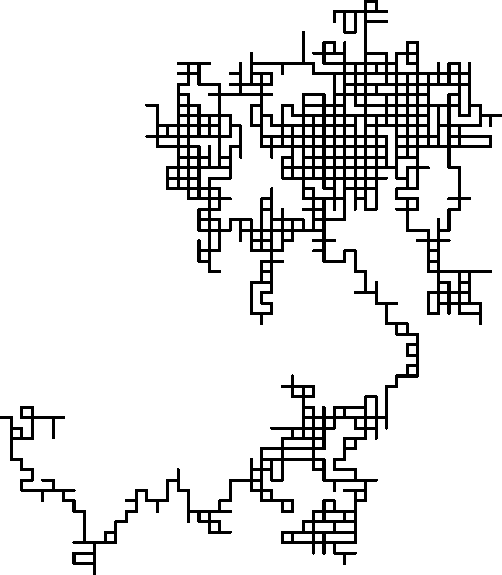
\includegraphics[width=0.25\textwidth]{images/randomwalk.pdf}
        \caption{Passeio aleatório (Wikipedia).}
        \label{fig:random_walk_2d}
        \end{figure}

  Vamos considerar aqui o exemplo do passeio aleatório sobre um grafo com pesos.
  \begin{itemize}
  \item Assuma uma distribuição estacionária irredutível e aperiódica.
  \item Considere o grafo $G=(V,E)$ com $m$ nós rotulados $\{1, 2, \ldots, m\}$ e arestas entre os nós com pesos $w_{ij} \geq 0$ 
	(aresta entre o nó $i$ e o nó $j$). Teremos $w_{ij} = w_{ji}$ e $w_{ij}=0$ se não existe aresta entre os nós $i$ e $j$.

        \begin{figure}[h!]
        \centering
        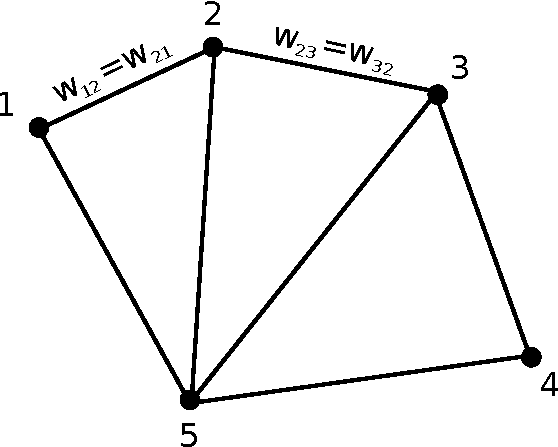
\includegraphics[width=0.3\textwidth]{images/grafo.pdf}
        \label{fig:grafo}
        \end{figure}

  \item O andar do bêbado (\textit{random walk}) $\{ X_n \}$, $X_n \in \{1,2,\ldots,m\}$, é uma sequência de vértices de um grafo.
  \item Dado $X_n = i$, o próximo vértice $j$ será escolhido dentre aqueles nós conectados com $i$ com probabilidade proporcional
	ao peso conectando os vértices $i$ e $j$, i.e., $p_{ij}$ será dado por
	\begin{equation}
	p_{ij} = \frac{w_{ij}}{\sum_j w_{ij}} = \frac{w_{ij}}{w_i}
	\end{equation}
	onde $w_i \triangleq \sum_j w_{ij}$ (peso total das arestas que saem do nó $i$).
  \item A soma de todos os pesos, de todas as arestas será dada por
	\begin{equation}
	w = \sum_{i,j : j > i} w_{ij}
	\end{equation}
  \item Note que $\sum_i w_i = \sum_{i,j} w_{ij} = 2w$.
  \item Vamos supor que a distribuição estacionária é dada por $\mu_i = \frac{w_i}{2w}$, o que poderemos
	checar verificando a equação $\mu^T = \mu^T P$:
	\begin{equation}
	\begin{pmatrix} \mu_1 & \mu_2 & \ldots & \mu_m \end{pmatrix} =  
		\begin{pmatrix} \mu_1 & \mu_2 & \ldots & \mu_m \end{pmatrix}
 		\begin{pmatrix}
		p_{11} & p_{12} & \ldots & p_{1m} \\
		p_{21} & p_{22} & \ldots & p_{2m} \\
		\vdots & \vdots & \ddots & \vdots \\
		p_{m1} & p_{m2} & \ldots & p_{mm}
		\end{pmatrix}
	\end{equation}
	ou seja,
	\begin{equation}
	\forall j, \quad \sum_i \mu_i p_{ij} = \sum_i \frac{w_i}{2w} \frac{w_{ij}}{w_i} = \sum_i \frac{1}{2w} w_{ij} = \frac{w_j}{2w} = \mu_j
	\end{equation}
  \item $\mu_j = \frac{w_j}{2w}$ : esta distribuição estacionária possui uma interessante propriedade de localização:
	ela depende apenas dos pesos locais (conectados ao nó em questão) e do total dos pesos; desta forma, ela não 
	sofrerá alteração se os pesos de uma outra parte do grafo (com arestas não ligadas ao nó $i$) 
	sofrerem alteração sem alterar a soma dos pesos.
  \item Note que a cadeia é aperiódica, já que $w_{ii} = 0$, como evidenciado abaixo
	\begin{eqnarray}
	2w &=& \sum_i w_i = \sum_{i,j} w_{ij} = \sum_{i,j : i=j} w_{i,j} + \sum_{i,j : i>j} w_{i,j} + \sum_{i,j : i<j} w_{i,j}  \nonumber \\
	&=& \sum_{i,j : i=j} w_{i,j} + w + w = \sum_{i,j : i=j} w_{i,j} + 2w
	\end{eqnarray}
 	logo, $\sum_{i,j : i=j} w_{i,j} = 0 \Rightarrow w_{ii} = 0$.
  \item A taxa de entropia para este passeio aleatório será dada por
	\begin{eqnarray}
	H(\mathcal{X}) &=& H(X_2 \mid X_1) = -\sum_i \mu_i \sum_j p_{ij} \log p_{ij} \nonumber \\
		&=& - \sum_i \frac{w_i}{2w} \sum_j \frac{w_{ij}}{w_i} \log \frac{w_{ij}}{w_i} = - \sum_{i,j} \frac{w_{ij}}{2w} \log \frac{w_{ij}}{w_i} \nonumber \\
		&=& - \sum_{i,j} \frac{w_{ij}}{2w} \log \left( \frac{w_{ij}}{w_i} \frac{2w}{2w} \right) \nonumber \\
		&=& - \sum_{i,j} \frac{w_{ij}}{2w} \log \frac{w_{ij}}{2w} - \sum_{i,j} \frac{w_{ij}}{2w} \log \frac{2w}{w_i} \nonumber \\
		&=& H\left( \ldots,\frac{w_{ij}}{2w} , \ldots \right) - H\left( \ldots,\frac{w_{i}}{2w} , \ldots \right) 
	\end{eqnarray}
	onde o primeiro termo representa a incerteza sob todas arestas e o segundo termo representa a incerteza sob todos os nós em condição estacionária
	($w_i/2w=\mu_i$).

	Se todas arestas possuírem o mesmo peso, sendo $E_i$ o número de arestas emanando do nó $i$, e $E$
	o número total de arestas, teremos
	\begin{equation}
	H(\mathcal{X}) = \log (2E) - H \left( \frac{E_1}{2E}, \frac{E_2}{2E}, \ldots, \frac{E_m}{2E} \right) .
	\end{equation}
  \end{itemize}
\end{frame}


\subsection{Cadeia Oculta de Markov}
\begin{frame}[allowframebreaks]
  \frametitle{Modelo de Markov}
        \begin{figure}[h!]
        \centering
        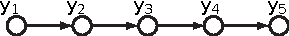
\includegraphics[width=0.4\textwidth]{images/mm.pdf}
        \label{fig:mm}
        \end{figure}
  Para o modelo de Markov de primeira ordem, temos que dois estados são independentes quando um intermediário é dado, por exemplo:
	\begin{equation}
	Y_5 \independent Y_3 \mid Y_4 \text{ ou então } Y_4 \independent Y_1 \mid Y_{2:3} \text{ ou } Y_4 \independent Y_1 \mid Y_2
	\end{equation}
\end{frame}


\begin{frame}[allowframebreaks]
  \frametitle{Cadeia Oculta Markov}
        \begin{figure}[h!]
        \centering
        \includegraphics[width=0.4\textwidth]{images/hmm.pdf}
        \label{fig:hmm}
        \end{figure}
  Na cadeia oculta de Markov, dizemos que um observação é gerada por um estado independente de outras observações ou estados passados.
  Por exemplo:
	\begin{equation}
        X_3 \independent X_1 \mid Y_3
        \end{equation}

  \framebreak

  \begin{itemize}
  \item Seja $Y_1, Y_2, \ldots, Y_n$ uma cadeia de Markov estacionária.
  \item Seja $X_{1:n}$ uma função aleatória desta cadeia de Markov, i.e.,
	\begin{equation}
	X_i = \phi_N (Y_i) = \begin{cases}
				\phi_1 (Y_i) \quad \text{com prob. } p_1(Y_i) \\
				\phi_2 (Y_i) \quad \text{com prob. } p_2(Y_i) \\
				\vdots \\
				\phi_m (Y_i) \quad \text{com prob. } p_m(Y_i) 
				\end{cases}
	\end{equation}
	onde $N \in \{1,2,\ldots,m\}$ é uma variável aleatória.
  \item Note que o processo estocástico $X_1,X_2,\ldots$ não forma uma cadeia de Markov. Sequer a Markovidade de primeira ordem é satisfeita.
	Por exemplo: não podemos falar que $X_4 \independent X_1 \mid X_{2:3}$, 
	mesmo conhecendo $X_{2:3}$, $X_1$ ainda pode ser necessário para determinar $X_4$.
  \item Se $\{Y_i\}_i$ é estacionário, então $\{X_i\}_i$ é um processo estacionário.
  \item A taxa de entropia do processo $\{X_i\}_i$ pode ser calculada
	\begin{equation}
	H(\mathcal{X}) = \lim_{n \rightarrow \infty} H(X_n \mid X_{n-1}, \ldots, X_1) 
	\end{equation}
	mas iremos calcular os limites inferior e superior, o que é mais simples.
  \item Limite superior:
	\begin{eqnarray}
	H(X_n \mid X_{n-1}, \ldots, X_1) &=& H(X_{n+1} \mid X_{n}, \ldots, X_2) \nonumber \\
		&\geq& H(X_{n+1} \mid X_{n}, \ldots, X_2, X_1) \nonumber \\
		&=& H(X_{n+2} \mid X_{n+1}, \ldots, X_2) \nonumber \\
		&\geq& H(X_{n+2} \mid X_{n+1}, \ldots, X_2, X_1) \nonumber \\
		&\geq& \ldots \geq H(\mathcal{X})
	\end{eqnarray}
  \item Limite inferior:
	\begin{eqnarray}
	H(X_n \mid X_{n-1}, \ldots, X_2, Y_1) = H(X_n \mid X_{n-1}, \ldots, X_2, X_1,Y_1) \nonumber \\
		\text{já que } X_n \independent X_1 \mid Y_1 \nonumber \\
		= H(X_n \mid X_{n-1}, \ldots, X_2, X_1,Y_1,Y_0,Y_{-1},\ldots,Y_{-k}) \\
		\text{já que } X_n \independent Y_0 \mid Y_1 \text{ e } X_n \independent Y_{-1} \mid Y_1 \text{ etc...} \nonumber \\
		= H(X_n \mid X_{n-1}, \ldots, X_2, X_1,Y_1,Y_0,Y_{-1},\ldots,Y_{-k},X_0,\ldots,X_{-k}) \nonumber \\
		\text{pelo mesmo motivo} \nonumber \\
		\leq H(X_n \mid X_{n-1}, \ldots, X_2, X_1,X_0,\ldots,X_{-k}) \nonumber \\
		\text{condicionar reduz a entropia} \nonumber \\
		= H(X_{n+k+1} \mid X_{n+k}, \ldots, X_1) \\
		\text{estacionariedade} \nonumber 
	\end{eqnarray}
 	Desta forma temos o limite inferior:
	\begin{equation}
	H(X_n \mid X_{n-1}, \ldots, X_2, Y_1) \leq H(\mathcal{X})
	\end{equation}
  \item Os limites para a taxa de informação em uma HMM são dados 
	\begin{equation}
        H(X_n \mid X_{n-1}, \ldots, X_1, Y_1) \leq H(\mathcal{X}) \leq H(X_n \mid X_{n-1}, \ldots, X_1)
	\end{equation}
  \end{itemize}


  \framebreak

  \begin{theorem}[teorema do confronto (sanduíche)]
  \begin{equation}
  H(X_n \mid X_{n-1}, \ldots , X_1) - H(X_n \mid X_{n-1}, \ldots, X_1, Y_1) \rightarrow 0
  \end{equation}
  \end{theorem}

  \begin{proof}
  \begin{eqnarray}
  H(X_n \mid X_{n-1}, \ldots , X_1) - H(X_n \mid X_{n-1}, \ldots, X_1, Y_1)  \nonumber \\
	= I(X_n ; Y_1 \mid X_{n-1}, \ldots, X_1) \leq H(Y_1)
  \end{eqnarray}
  Temos também que $I(Y_1 ; X_1, \ldots, X_n) \leq H(Y_1)$, para todo $n$.
  \proofbreak
  Utilizando a regra da cadeira da informação mútua ($I(X;Y,Z) = I(X;Z) + I(X;Y|Z)$), e tirando o limite, teremos
  \begin{eqnarray}
  \lim_{n \rightarrow \infty} I(Y_1 ; X_1, \ldots, X_n) =  \lim_{n \rightarrow \infty} \sum_{i=1}^n I(Y_1;X_i \mid X_{1:i-1}) \nonumber \\
	= \sum_{i=1}^\infty I(Y_1;X_i \mid X_{1:i-1}) \leq H(Y_1) < \infty
  \end{eqnarray} 
  Então o resultado da soma infinita é uma constante, isto significa que os termos $\rightarrow 0$ quando $n \rightarrow \infty$.
  Logo, cada um dos termos $I(Y_1;X_i \mid X_{1:i-1}) \rightarrow 0$ quando $n \rightarrow \infty$.
  \end{proof}

  \framebreak

  Ao final, temos que
  \begin{equation}
  \lim_{n \rightarrow \infty} H(X_n \mid X_{n-1}, \ldots, X_1, Y_1) = H(\mathcal{X}) = \lim_{n \rightarrow \infty} H(X_n \mid X_{n-1}, \ldots, X_1)
  \end{equation}
\end{frame}


% códigos
\section{Codificação}

\begin{frame}[allowframebreaks]
  \frametitle{Codificação}
  \begin{itemize}
  \item Codificação sem perdas de informação de fontes regidas por uma determinada distribuição.
  \item Teorema da Codificação de Shannon: é possível codificar utilizando $R > H(X)$ bits por
	símbolo da fonte, se utilizarmos bloco grande suficiente.
  \item Transmissão de blocos não é prática.
  \item Outras alternativas:
	\begin{enumerate}
	\item Códigos de tamanho variável: os símbolos são codificados separadamente utilizando
		palavras de código com comprimento variável. Ex: Codificação Huffman.
	\item Codificação de Fluxo (\textit{stream code}): codificação que opera no fluxo de dados,
		decidindo a palavra código dependendo do símbolo corrente e da história 
		(símbolos passados). Ex: Codificação Aritmética, Codificação Lempel-Ziv
		(sendo este ultimo um codificação universal, pois não requer $p(x)$).
	\end{enumerate}
  \item Queremos uma codificação prática que alcance o limite da entropia.
  \item A codificação pode utilizar a distribuição $p(x)$ dada, ou estimá-la de alguma forma.
  \item Não iremos lidar aqui com o problema de estimar $p(x)$ (problema de estimação de densidade),
	vamos supor que $p(x)$ é conhecido ou sua aproximação $q(x)$ é dada.
  \item Vamos verificar o efeito de utilizar a aproximação $q(x)$ quando a distribuição subjacente é $p(x)$.
  \end{itemize}
\end{frame}

\begin{frame}[allowframebreaks]
  \frametitle{Codificação de Fonte}
  \begin{definition}[Codificação de Fonte]
  Um código $C$ para a v.a. $X$ é um mapeamento de $\mathcal{X}$ em $\mathcal{D}^\ast$, 
  ou seja 
	\begin{equation} 
	C: \mathcal{X} \rightarrow \mathcal{D}^\ast , 
	\end{equation} 
  onde $\mathcal{D}^\ast$ é o conjunto
  de sequências (\textit{strings}) finitas em um alfabeto $D$-ário. $C(x)$ é a palavra código 
  (\textit{codeword}) correspondente ao símbolo $x$, e $l(x)$ é o comprimento desta palavra.
  \end{definition}

  \begin{example}
  Seja $\mathcal{X} = \{\text{azul}, \text{vermelho}\}$. O código pode ser $C(\text{vermelho})=00$ e 
  $C(\text{azul})=11$, o que seria um código binário para $\mathcal{D} = \{0,1\}$.
  Teríamos então $\mathcal{D}^\ast = \{ 00 , 11 \}$. Uma sequência produzida pela fonte da forma
  $(\text{azul},\text{azul},\text{vermelho})$ seria codificada como $(11,11,00)$, ou melhor, $111100$.
  \end{example}

  \framebreak

  \begin{definition}[Comprimento Esperado]
  O comprimento esperado $L(C)$ de um código $C$ para uma v.a. $X$ com distribuição $p(x)$ é dado por
	\begin{equation}
	L(C) = \sum_x p(x) l(x)
	\end{equation}
  \end{definition}

  \framebreak

  \begin{itemize}
  \item De forma geral, $\mathcal{D} = \{0,1, \ldots, D-1\}$, mas usualmente utilizamos $D=2$.
  \end{itemize}
  \begin{example}
     \begin{columns}
     \begin{column}{0.45\textwidth}
	Seja $\mathcal{X} = \{1, 2, 3, 4\}$ e $\mathcal{D} = \{0, 1\}$. Podemos definir 
	o código através da tabela.
     \end{column}
     \begin{column}{0.45\textwidth}
	\begin{tabular}{c|c|c|c}
	x & p(x)  & c(x) & l(x) \\ \hline
	1 & $1/2$ & 0    & 1	\\
	2 & $1/4$ & 10   & 2	\\
	3 & $1/8$ & 110  & 3	\\
	4 & $1/8$ & 111  & 3	\\
	\end{tabular}
     \end{column}
     \end{columns}
    \examplebreak
    \begin{itemize}
    \item Neste caso, teremos $H(X) = 1.75$ e $L(C)=El(X)=1.75$, então este código é muito bom.
    \item A decodificação para este código é fácil.
    \item Qual é a sequência de símbolos que produziu a seguinte sequência 010110111111110100? R: 1,2,3,4,4,3,2,1.
    \item Com pontuação separando os símbolos: 0,10,110,111,111,110,10,0. Dizemos que o código possui pontuação
	automática.
    \end{itemize}
  \end{example}

  \framebreak

  \begin{example}
  Vamos considerar $\mathcal{X} = \{1,2,3\}$ e $\mathcal{D}=\{0,1\}$.
 
  Código:
  \begin{tabular}{cccc}
  x      &  1    &   2   &   3   \\ \hline
  $p(x)$ & $1/3$ & $1/3$ & $1/3$ \\ \hline
  $C(X)$ & $0$   & $10$  & $11$  
  \end{tabular}

  Teremos então $H = 1.58$bits e $El(X)=1.66 > H$ bits.
  \end{example}

  Podemos facilmente decodificar? Por exemplo: $10110010 = 2,3,1,1,2$.


  \framebreak


  \begin{figure}[h!]
  \centering
  \includegraphics[width=0.4\textwidth]{images/International_Morse_Code.pdf}
  \label{fig:International_Morse_Code}
  \end{figure}

  \begin{itemize}
  \item Note que um código pode ser um prefixo de outro.
  \end{itemize}

  \framebreak

  Para $\mathcal{X} = \{1,2,3,4\}$ e $\mathcal{D}=\{0,1\}$ (código binário), considere os seguintes códigos

  \begin{center}
  \begin{tabular}{c|c|c|c|c|c}
  $x$ 		& $p(x)$& $C_I$ & $C_{II}$ & $C_{III}$ & $C_{IV}$ \\ \hline
  1		& 0.5	&  0	&   0	&  0 		&   0	\\ 
  2		& 0.25	&  0	&   1 	& 10		&  01	\\
  3		& 0.125	&  1	&  00	& 110		& 011 	\\
  4		& 0.125	& 10	&  11	& 111 		& 0111 	\\
  $H(X)$	& 1.75	&  -	&  -	&  -		&  -	\\
  $El(X)$ 	&  -	& 1.125	& 1.25	&  1.75		& 1.875
  \end{tabular}
  \end{center} 

  \begin{itemize}
  \item Eficiência do Código = $H(X) / El(X)$.
  \item Geralmente preferimos códigos com comprimento esperado menor.
  \item Note que o código $C_I$ não é unívoco. A sequência $00001$ pode ser decodificada como
	$1,2,1,2,3$ ou $2,1,2,1,3$ ou $1,1,1,1,3$ ...
  \item O valor esperado do comprimento do código não pode ser menor que a entropia sem que o código
	incorra em erro.
  \item Considere $C_{II}$. Qual seria o resultado da decodificação de $0011$? Poderia ser
	$,1,1,2,2$ ou $3,4$ ou $3,2,2$ ou $1,1,4$. Novamente, não é possível decodificar sem
	que a probabilidade de erro seja nula (quando a sequência torna-se mais longa, a probabilidade
	de erro tende a $1$).
  \item O código $C_{III}$ é factível (já que $El \geq H$). O processo de decodificação é simples.
	Por exemplo: $111110100 = 111,110,10,0 = 4,3,2,1$.
  \item Utilizando o código $C_{IV}$ é possível decodificar a sequência $00000000111$? Sim, mas 
	os símbolos não são instantaneamente decodificados, é necessário ver os bits à frente para 
	conseguir decodificar.
  \end{itemize}
 
\end{frame}



\subsection{Tipos de Código}
\begin{frame}[allowframebreaks]
  \frametitle{Tipos de Código}

  \begin{definition}[extensão]
  Um extensão $C^\ast$ de um código $C$ é um mapeamento de uma sequência finita 
  de símbolos em $\mathcal{X}$ em uma sequência finita de símbolos em $\mathcal{D}$ através da
  concatenação dos códigos: 
  	\begin{equation}
	C^\ast (x_1,x_2,\ldots,x_n) = C(x_1) C(x_2) \ldots C(x_n)
	\end{equation}
  \end{definition}
  \begin{example}
  Se $C(x_1)=0$ e $C(x_2)=1$, então $C(x_1,x_2) = 01$.
  \end{example}
  \begin{example}
  Se $C(x_1)=000$ e $C(x_2)=100$, então $C(x_1,x_2,x_2) = 000100100$.
  \end{example}

  \framebreak

  \begin{definition}[não-singular]
  Um código é dito \textbf{não-singular} se todo elemento de $\mathcal{X}$
  é mapeado em sequências (\textit{strings}) diferentes em $\mathcal{D}^\ast$. I.e.,
	\begin{equation}
	x_i \neq x_j \Rightarrow C(x_i) \neq C(x_j)
	\end{equation}
  \end{definition}

  \begin{figure}[h!]
  \centering
  \includegraphics[width=0.5\textwidth]{images/nonsingularmap2.pdf}
  \label{fig:nonsingularmap}
  \end{figure}

  \framebreak

  \begin{definition}[decodificação unívoca]
  Um código $C$ com extensão $C^\ast$ é decodificável univocamente se a sua extensão $C^\ast$ for não-singular.
  \end{definition}
  
  \begin{itemize}
  \item Objetivo: transmitir ou armazenar uma sequência de símbolos na forma de uma sequência de palavras codificadas.
  \item Um código não-singular pode se tornar único se inserirmos pontuação, mas para isto seria necessário incluir
	um novo símbolo no alfabeto $\mathcal{D}$, o que aumentaria a taxa $R$.
  \item É preferível um código com característica de auto-pontuação e que seja instantâneo.
  \end{itemize}

  \framebreak

  Considere o código

  \begin{center}
  \begin{tabular}{ccccc}
  $x$    & 1  & 2  & 3  & 4 \\ \hline
  $C(x)$ & 10 & 00 & 11 & 110
  \end{tabular}
  \end{center}

  \begin{itemize}
  \item Este código é unicamente decodificável.
  \item Ex.: 1100000000 = 3,2,2,2,2.
  \item Ex.: 11000000000 = 4,2,2,2,2.
  \item Note que só sabemos a identidade do primeiro símbolo após ler toda a sequência.
  \end{itemize}

  \framebreak

  \begin{definition}[código de prefixo]
  Um código é chamado \textbf{código de prefixo} ou \textbf{código instantâneo} se nenhum palavra
  é prefixo de qualquer outra palavra.
  \end{definition}

  \begin{itemize}
  \item Quando temos um código de prefixo, sabemos onde está o fim de uma palavra, pois ela não
	é prefixo de nenhuma outra, ou seja, não existe nenhuma outra palavra que comece com a palavra
	encontrada.
  \item Um código de prefixo possui então a propriedade de auto-pontuação.
  \item Código de prefixo $\Rightarrow$ unicamente decodificável. 
	Mas unicamente decodificável $\nRightarrow$ código de prefixo.
  \end{itemize}
 
  \framebreak

  \begin{figure}[h!]
  \centering
  \includegraphics[width=0.75\textwidth]{images/tiposcodigos.pdf}
  \label{fig:tiposcodigos}
  \end{figure}

  \begin{itemize}
  \item Queremos um código com comprimento esperado mínimo possível.
  \item Analisando as classes de códigos, intuitivamente pensamos que é mais provável encontrarmos
	um código com comprimento esperado menor em uma classe maior (ou mais abrangente).
  \item Podemos alcançar um resultado melhor que a entropia se não utilizarmos um código não-singular,
	entretanto, queremos uma codificação sem perda.
  \end{itemize} 
\end{frame}



\subsection{Desigualdade de Kraft}
\begin{frame}[allowframebreaks]
  \frametitle{Desigualdade de Kraft}

  \begin{theorem}[Desigualdade de Kraft]
  Para qualquer código instantâneo (código de prefixo) sobre um alfabeto de tamanho $D$, o comprimento
  das palavras $l_1, l_2, \ldots, l_m$ deve satisfazer 
	\begin{equation}
	\sum_i D^{-l_i} \leq 1 .
	\end{equation}
  Por um outro lado, dado um conjunto de comprimentos de código satisfazendo a desigualdade acima,
  então existe um código de prefixo com estes comprimentos.
  \end{theorem}

  \begin{itemize}
  \item Note que foi dito que existe um código de prefixo com aqueles comprimentos, não significa que todos códigos
	cujos comprimentos satisfazem a desigualdade são códigos de prefixo.
  \item Se existe um código não-instantâneo com comprimentos $l_i$ satisfazendo a desigualdade de Kraft, então
	podemos encontrar um outro código, que terá a propriedade de prefixo, e que possuirá os mesmos comprimentos $l_i$,
	consequentemente não alterando o comprimento esperado.
  \item Logo, será sempre melhor escolher um código de prefixo.
  \end{itemize}

  \framebreak

  \begin{proof}[Desigualdade de Kraft]
  Vamos representar o conjunto de códigos em uma árvore $D$-ária (não necessariamente balanceada).

  \begin{figure}[h!]
  \centering
  \includegraphics[width=0.5\textwidth]{images/Dtree.pdf}
  \label{fig:Dtree}
  \end{figure}
  
  \proofbreak

  \begin{itemize}
  \item As palavras correspondem à folhas na árvore.
  \item O caminho da raiz até a folha determina a palavra código.
  \item A condição de prefixo implica que não existe uma palavra a não ser nas folhas 
	(nenhum descendente de uma palavra código será também uma palavra código).
  \item $l_{\text{max}} = \max_i (l_i)$ é o comprimento da palavra mais longa.
  \item Podemos expandir toda a árvore até o comprimento $l_{\text{max}}$.
  \item Os nós no nível de $l_{\text{max}}$ são:
	\begin{enumerate}
	\item palavras de código;
	\item descendentes de palavras de código; ou
	\item nem um, nem outro.
	\end{enumerate}
  \end{itemize}
  \proofbreak
  \begin{itemize}
  \item Considere uma palavras $i$ no nível $l_i$ da árvore (então esta palavra possui comprimento $l_i$).
  \item Existem então $D^{l_{\text{max}} - l_i}$ descendentes de $i$, na árvore, no nível $l_{\text{max}}$.
  \item Com a condição de prefixo, podemos afirmar que os descendentes de código $i$ no nível $l_i$ são
	disjuntos dos descendentes do código $j$ no nível $l_j$, quando $i \neq j$ (i.e., o conjunto de
	descendentes para diferentes palavras é disjunto).
  \item O número total de nós em um conjunto de todos descendentes é $\leq D^{l_{\text{max}}}$.
  \end{itemize}
  \proofbreak
  \begin{itemize}
  \item Utilizando o que vimos acima, temos que a soma do número de descendentes de todos os códigos é menor ou
	igual ao número de folhas na árvore cheia no nível $l_{\text{max}}$. Podemos então escrever
	\begin{equation}
	\sum_i D^{l_{\text{max}} - l_i} \leq D^{l_{\text{max}}} \quad \Rightarrow \quad \sum_i D^{-l_i} \leq 1
	\end{equation}
  \item Por outro lado, dados os comprimentos $l_1, l_2, \ldots, l_m$, satisfazendo Kraft, iremos mostrar como
	construir um código de prefixo utilizando estes comprimentos.
  \item Considere uma árvore $D$-ária cheia de profundidade $l_{\text{max}}$ e $D^{l_{\text{max}}}$ nós terminais.
  \end{itemize}
  \proofbreak
  \begin{itemize}
  \item Observe que
	\begin{enumerate}
	\item No nível 0 existe uma fração $1$ de descendentes de cada nó neste nível;
	\item No nível 1 existe uma fração $1/D$ de descendentes de cada nó neste nível;
	\item No nível 2 existe uma fração $1/D^2$ de descendentes de cada nó neste nível;
	\item ...
	\end{enumerate}
  \item De forma geral, em cada nível $i \in [0, l_{\text{max}}]$ da árvore, existe uma fração de $D^{-i}$
	nós terminais que são descendentes de uma ramificação de cada um dos $D^i$ nós no nível $i$.
  \end{itemize}
  \proofbreak
  \begin{itemize}
  \item Ordene então os comprimentos $(l_1, l_2, \ldots, l_m)$ de forma ascendente $(s_1, s_2, \ldots, s_m)$, 
	sendo $s_1 \leq s_2 \leq \ldots \leq s_m$. Observe que existem tantos comprimentos quanto existem palavras.
  \item Para o comprimento $s_1$, escolha um nó no nível $s_1$ para indicar o código.
  \item Para garantir a condição de prefixo, o nó escolhido deve se tornar um nó terminal, eliminando assim uma
	fração $D^{-s_1}$ de nós terminais no nível $l_{\text{max}}$.
  \item Em seguida, escolha um dos nós remanescentes no nível $s_2$ (neste momento, existem $(D^{s_1}-1)D^{s_2-s_1}$
	possíveis escolhas), eliminando assim uma fração $D^{-s_2}$ de nós terminais no nível $l_{\text{max}}$.
  \end{itemize}
  \proofbreak
  \begin{itemize}
  \item A fração total de nós eliminados, até o momento, foi de $D^{-s_1} + D^{-s_2}$.
  \item Continuando este processo, iremos eliminar uma fração $\sum_{i=1}^{m} D^{-s_i}$ de nós, e neste processo
	estamos garantindo que estamos criando um código instantâneo (uma palavra de código não pode ser prefixo de outra).
  \item Como por suposição temos $\sum_{i=1}^{m} D^{-s_i} \leq 1$, nunca iremos eliminar mais do que todas as palavras
	de código, então este processo não irá exaurir as palavras de código.
  \item Criamos assim um código de prefixo com os comprimentos desejados, satisfazendo Kraft.
  \end{itemize}

  \end{proof}
\end{frame}


\begin{frame}[allowframebreaks]
  \frametitle{Kraft Infinito}

  \begin{theorem}[Kraft infinito contável]
  Para qualquer conjunto infinito contável de palavras de código que formam um conjunto com prefixo,
  este conjunto satisfaz a desigualdade de Kraft estendida, i.e.
	\begin{equation}
	\sum_{i=1}^{\infty} D^{-l_i} \leq 1
	\end{equation}
  Por outro lado, dados $l_i$s satisfazendo a equação acima, existe um código de prefixo com estes comprimentos.
  \end{theorem}

  \framebreak

  \begin{proof}[Kraft Infinito]
  \begin{itemize}
  \item Assuma que tenhamos um código de prefixo infinito contável e que o alfabeto é $D$-ário $\{0,1,\ldots,D-1\}$.
  \item Considere a $i$-ésima palavra $y_1,y_2,\ldots,y_{l_i}$.
  \item A expansão da $i$-ésima palavra, de comprimento $l_i$, utilizando os dígitos fracionários é da forma
	\begin{equation}
	0.y_1 y_2 y_3 \ldots y_{l_i} = \sum_{j=1}^{l_i} y_j D^{-j}
	\end{equation}
  \end{itemize}
  \proofbreak
  \begin{itemize}
  \item Considere os exemplos com $D=2$ e $\mathcal{D} = \{0,1\}$:
  	\begin{itemize}
	\item $0.1 = 1 \times 2^{-1} = \frac{1}{2}$
 	\item $0.01 = 0 \times 2^{-1} + 1 \times 2^{-2} = \frac{1}{4}$
	\item $0.11 = 1 \times 2^{-1} + 1 \times 2^{-2} = \frac{3}{4}$
	\item $0.001 = 1 \times 2^{-1} + 1 \times 2^{-2} + 1 \times 2^{-3} = \frac{1}{8}$
	\end{itemize}
  \item Vamos associar cada palavra $y_{1:l_i}$ com o intervalo semiaberto na reta real
	$[0.y_1 y_2 \ldots y_{l_i} , 0.y_1 y_2 \ldots y_{l_i} + 1/D^{l_i} )$.
  \end{itemize}
  \proofbreak
  \begin{itemize}
  \item Considere os exemplos com $D=2$ e $\mathcal{D} = \{0,1\}$:
	\begin{itemize}
        \item A palavra $0.y_1 = 0.1 = \frac{1}{2}$ está associada ao intervalo $[\frac{1}{2}, 1)$.
	\item A palavra $0.y_1 y_2 = 0.01 = \frac{1}{4}$ está associada ao intervalo $[\frac{1}{4}, \frac{1}{2})$.
	\item A palavra $0.y_1 y_2 y_3= 0.001 = \frac{1}{8}$ está associada ao intervalo $[\frac{1}{8}, \frac{1}{4})$.
        \end{itemize}
	Considere agora os exemplos seguintes com $D=10$.
	\begin{itemize}
        \item $0.y_1 y_2 y_3 = 0.157$ está associado ao intervalo $[0.157, 0.158)$.
	\item $0.y_1 y_2 y_3 = 0.159$ está associado ao intervalo $[0.159, 0.160)$.
	\end{itemize}
	  \begin{figure}[h!]
	  \centering
	  \includegraphics[width=0.5\textwidth]{images/kraftintervals2.pdf}
	  \label{fig:kraftintervals}
	  \end{figure}
  \end{itemize}
  \proofbreak
  \vspace{-0.2cm}
  \begin{itemize}
  \item O intervalo da palavra $y_1 y_2 \ldots y_{l_i}$ corresponde ao conjunto de todos números que iniciam-se com
	$y_1 y_2 \ldots y_{l_i}$, e desta forma é um subintervalo do intervalo unitário.
  \item Além disso, $y_1 y_2 \ldots y_{l_i}$ não é prefixo para nenhuma outra palavra, desta forma os intervalos
	serão disjuntos.
  \item O tamanho do intervalo associado à palavra $y_1 y_2 \ldots y_{l_i}$ é $D^{-l_i}$.
  \item Como todos intervalos estão dentro do intervalo $[0,1)$ teremos que
	\begin{equation}
	\sum_i D^{-l_i} \leq 1
	\end{equation}
  \vspace{-0.2cm}
  \item A prova da proposição inversa é similar ao caso finito.
  \end{itemize}
  \end{proof}
\end{frame}


\subsection{Código Ótimo}
\begin{frame}[allowframebreaks]
  \frametitle{Em busca de um código ótimo}
  \begin{itemize}
  \item Código de prefixo $\Leftrightarrow$ desigualdade de Kraft.
  \item Precisamos encontrar os comprimentos $l_i$ que satisfazem Kraft para obter um código de prefixo.
  \item Objetivo: encontrar um código de prefixo com o comprimento esperado mínimo.
	\begin{equation}
	L(C) = \sum_{i} p_i l_i
	\end{equation}
  \item Temos então um problema de otimização com restrição:
	encontrar
	\begin{equation}
	\min_{\{l_{1:m}\} \in \mathbb{Z}_{+}^m} \sum_i p_i l_i
	\end{equation}
	sujeito a
	\begin{equation}
	\sum_i D^{-l_i} \leq 1
	\end{equation}
  \item Temos um problema de programação em inteiros que é um problema NP-difícil. Este problema
	não provável de ser solucionado eficientemente (a menos que $P=NP$). 
  \item Vamos relaxar a condição de que $l_i$ precisa ser inteiro e considerar o Lagrangiano
	\begin{equation}
	J = \sum_i p_i l_i + \lambda \left( \sum_i D^{-l_i} - 1 \right)
	\end{equation}
  \item Tomando as derivadas e igualando a zero, teremos:
	\begin{eqnarray}
	\frac{\partial J}{\partial l_i} = p_i - \lambda D^{-l_i} \ln D = 0 \nonumber \\
	\Rightarrow D^{-l_i} = \frac{p_i}{\lambda \ln D}
	\end{eqnarray}
  	\begin{equation}
	\frac{\partial J}{\partial \lambda} = \sum_i D^{-l_i} - 1 = 0 \Rightarrow \lambda = 1 / \ln D
	\end{equation}
	\begin{equation}
	\Rightarrow D^{-l_i} = p_i \quad \text{implicando em} \quad l^\ast_i = -\log_D p_i
        \end{equation}
  \item Isto implica que
	\begin{equation}
	L^\ast = \sum_i p_i l_i^\ast = - \sum_i p_i \log_D p_i = H_D (X) = H(X) / \log D
	\end{equation}
  \item Os comprimentos ótimos para as palavras de um código são, de acordo com a otimização realizada,
	dados pela entropia, assumindo que seja possível utilizar comprimentos fracionários.
  \item Como $l^\ast_i = - \log_D p_i$, isto implica que os ``comprimentos'' ótimos (mesmo que fracionários)
	são iguais à informação do evento. I.e., o menor comprimento para codificação é inerentemente a informação
	sobre este evento (princípio da descrição mínima - Navalha de Occam).
  \item Com a codificação em blocos podemos aproximar do limite ótimo em que os comprimentos dos códigos por símbolos
	são valores fracionários.
  \end{itemize}
\end{frame}
\note{
\textbf{NP-Difícil}

``Um problema H é NP-difícil se e somente se (sse) existe um problema NP-completo L 
que é Turing-redutível em tempo polinomial para H (i.e., L?=?TH). Em outras palavras, 
L pode ser resolvido em tempo polinomial por uma Máquina de Turing não determinística 
com um oráculo para H. Informalmente, podemos pensar em um algoritmo que pode chamar 
tal Máquina de Turing Não-Determinística como uma sub-rotina para resolver H, e resolver L 
em tempo polinomial, se a chamada da sub-rotina leva apenas um passo para computar. 
Problemas NP-difíceis podem ser de qualquer tipo: problemas de decisão, problemas de 
pesquisa ou problemas de otimização.'' (Wikipedia)
}
\note{
``Em problemas de otimização, o método dos multiplicadores de Lagrange permite encontrar 
extremos (máximos e mínimos) de uma função de uma ou mais variáveis suscetíveis a uma ou mais restrições.

Por exemplo, considere o problema de otimização:
\begin{itemize}
\item maximize $f(x,y)$ ou seja, deseja-se encontrar o ponto máximo desta função
\item sujeito a $g(x,y) = c$.
\end{itemize}

    \begin{figure}[h!]
    \centering
    \includegraphics[width=0.4\textwidth]{images/LagrangeMultipliersEx2.pdf}
    \label{fig:LagrangeMultipliersEx}
    \end{figure}
}
\note{
O método consiste em introduzir uma variável nova ($\lambda$ normalmente), 
chamada de multiplicador de Lagrange. A partir disso, estuda-se a função de Lagrange, assim definida:
\begin{equation}
\Lambda(x,y,\lambda) = f(x,y) + \lambda \cdot \Big(g(x,y)-c\Big),
\end{equation}

Nesta função, o termo $\lambda$ pode ser adicionado ou subtraído. Se $f(x,y)$ é um ponto de máximo 
para o problema original, então existe um $\lambda$ tal que $(x,y,\lambda)$ é um ponto estacionário 
para a função lagrangiana, ou seja, existe um ponto para o qual as derivadas parciais de $\Lambda$
são iguais a zero.

No entanto, nem todos os pontos estacionários permitem uma solução para o problema original. 
Portanto, o método dos multiplicadores de Lagrange garante uma condição necessária para a 
otimização em problemas de otimização com restrição.'' (Wikipedia)
}
\note{
\textbf{Navalha de Occam}

``A Navalha de Occam ou Navalha de Ockham é um princípio lógico atribuído ao lógico 
e frade franciscano inglês Guilherme de Ockham (século XIV).

O princípio afirma que a explicação para qualquer fenómeno deve supor apenas as premissas 
estritamente necessárias à sua explicação e eliminar todas as que não causariam qualquer 
diferença aparente nas predições da hipótese ou teoria. O princípio é frequentemente designado 
pela expressão latina \textit{Lex Parsimoniae} (Lei da Parcimónia) enunciada como: 
\textit{``entia non sunt multiplicanda praeter necessitatem''} (as entidades não devem ser 
multiplicadas além da necessidade).

O princípio recomenda assim que se escolha a teoria explicativa que implique o menor número 
de premissas assumidas e o menor número de entidades.
}


\begin{frame}[allowframebreaks]
  \frametitle{Código Ótimo}
  \begin{theorem}
  Entropia é o comprimento esperado mínimo. O comprimento esperado $L$ de qualquer código
  $D$-ário instantâneo (satisfaz Kraft por conseguinte) para uma v.a. $X$ é tal que
	\begin{equation}
	L \geq H_D (X)
	\end{equation}
  com igualdade sse $D^{-l_i} = p_i$.
  \end{theorem}

  \framebreak

  \begin{proof}
  \begin{eqnarray}
  L - H_D (X) &=& \sum_i p_i l_i - \sum_i p_i \log_D 1/p_i \nonumber \\
		&=& - \sum_i p_i \log_D D^{-l_i} + \sum_i p_i \log_D p_i 
  \end{eqnarray}
  \proofbreak
  \begin{eqnarray}
  L - H_D (X) &=& \ldots \nonumber \\
		&=& - \sum_i p_i \log_D D^{-l_i} + \nonumber \\
		&& \underbrace{ \log_D \left( \sum_i D^{-l_i} \right) - \log_D \left( \sum_i D^{-l_i} \right)  }_{=0} + \nonumber \\
		&& \sum_i p_i \log_D p_i 
  \end{eqnarray}

  \proofbreak
  {\scriptsize (interlúdio)}
  \vspace{-0.6cm}
  \begin{eqnarray}
  - \sum_i p_i \log_D D^{-l_i} + \log_D \left( \sum_j D^{-l_j} \right) +  \sum_i p_i \log_D p_i = \nonumber \\
  - \sum_i p_i \log_D D^{-l_i} + \left( \underbrace{ \sum_i p_i }_{=1} \right) \log_D \left( \sum_i D^{-l_i} \right) + \sum_i p_i \log_D p_i = \nonumber \\
  - \sum_i p_i \log_D D^{-l_i} + \sum_i p_i \log_D \left( \sum_j D^{-l_j} \right) + \sum_i p_i \log_D p_i = \ldots
  \end{eqnarray}
  \proofbreak
  \begin{eqnarray}
  \ldots &=&  \sum_i p_i \log_D \frac{p_i \left( \sum_j D^{-l_j} \right)}{D^{-l_i}} \nonumber \\
   	&=&  \sum_i p_i \log_D \frac{p_i}{\frac{D^{-l_i}}{\left( \sum_j D^{-l_j} \right)}} = \sum_i p_i \log_D \frac{p_i}{r_i}
  \end{eqnarray}
  onde definimos 
	\begin{equation}
	r_i = \frac{D^{-l_i}}{\sum_j D^{-l_j}} .
	\end{equation}
  \proofbreak
  Teremos assim
  \vspace{-0.3cm}
  \begin{eqnarray}
  L - H_D (X) &=& \ldots \nonumber \\
		&=& \sum_i p_i \log_D \frac{p_i}{r_i} - \log_D \left( \sum_i D^{-l_i} \right) \nonumber \\
		&=& \underbrace{D(p \mid\mid r)}_{ \geq 0} + \underbrace{\log_D (1/c)}_{ \geq 0} \nonumber \\
		&\geq& 0 \\
		&& \text{ já que } c \leq 1 \text{ pois satisfaz Kraft, } \nonumber \\
		&& \quad \quad \text{ onde } c = \sum_i D^{-l_i}. \nonumber
  \end{eqnarray}
  \end{proof}

  \begin{itemize}
  \item Mostramos que $L \geq H_D (X)$.
  \item A igualdade $L=H$ é alcançada sse $p_i = D^{-l_i}$ para todo $i$ sse $-\log_D p_i$ for um inteiro. Neste caso 
	teremos $c = \sum_i D^{-l_i} = 1$.
  \end{itemize}

  \begin{definition}[$D$-ádico]
  Uma distribuição probabilística é $D$-ádica com relação a $D$ se cada uma das probabilidades é da forma $D^{-n}$
  para algum $n$.
  \end{definition}
  \begin{itemize}
  \item Exemplo: Quando $D=2$, a distribuição $\left[ \frac{1}{2}, \frac{1}{4}, \frac{1}{8}, \frac{1}{8} \right] = [2^{-1}, 2^{-2}, 2^{-3}, 2^{-3}]$ é $2$-ádica.
  \item Teremos $L=H$ quando a distribuição for $D$-ádica.
  \end{itemize}
\end{frame}

\begin{frame}[allowframebreaks]
  \frametitle{Sumário}
  \begin{itemize}
  \item No problema de otimização relaxado, retiramos a restrição de que os comprimentos dos códigos
	precisam ser inteiros, desta forma obtivemos $E l = H$.
  \item Assumindo que Kraft seja satisfeito (existe um código de prefixo com tais comprimentos)
	teremos comprimentos inteiros de forma que $E l \geq H$. 
	\begin{itemize}
	\item Se ainda $l_i = -\log_D p_i$ é
	inteiro, para todo $i$, então teremos a igualdade $E l = H$. 
	\item Se $l_i \neq -\log_D p_i$, mas $l_i$ é inteiro, teremos estritamente $E l > H$.
	\end{itemize}
  \end{itemize}
\end{frame}


\subsection{Códigos de Shannon}
\begin{frame}[allowframebreaks]
  \frametitle{Como construir um código buscando o ótimo}
  \begin{itemize}
  \item Vimos anteriormente que o limite ótimo para o comprimento esperado do código é a entropia. Desta forma
	$L-H$ é uma medida do quão distante estamos deste ponto ótimo.
  \item $L-H = D(p \mid \mid r) + \log_D 1/c$, onde $c = \sum_i D^{-l_i}$ e $r_i = \frac{D^{-l_i}}{\sum_j D^{-l_j}}$.
  \item Para criar o código devemos buscar a distribuição $D$-ádica mais próxima (em termos de divergência de KL)
	da distribuição $p$ e então construir um código seguindo a proposição inversa de Kraft.
  \item De forma geral, a menos que $P=NP$, é difícil encontrar a distribuição $D$-ádica mais próxima (no sentido de KL)
	da distribuição $p$ (problema de programação linear).
  \end{itemize}
\end{frame}


\begin{frame}[allowframebreaks]
  \frametitle{Códigos de Shannon}
  \begin{itemize}
  \item Considerar o comprimento como inteiro mais próximo do valor ótimo: $l_i = \lceil \log_D 1/p_i \rceil$.
  \item Devemos verificar se esta escolha satisfaz Kraft:
	\begin{equation}
	\sum_i D^{-l_i} = \sum_i D ^{- \lceil \log_D 1/p_i \rceil} \leq \sum_i D^{-\log_D 1/p_i} = \sum_i p_i = 1
	\end{equation}
	Kraft é satisfeito, então existe um código de prefixo com estes comprimentos.
  \item Temos então os seguintes limites para os comprimentos:
	\begin{equation}
	\log_D \frac{1}{p_i} \leq l_i \leq \log_D \frac{1}{p_i} + 1
	\end{equation}
  \item Tomando o valor esperando teremos:
	\begin{eqnarray}
	E_p \left[ \log_D \frac{1}{p_i} \right]  & \leq E_p \left[ l_i \right] \leq E_p & \left[ \log_D \frac{1}{p_i} + 1 \right] \nonumber \\
	\sum_i p_i \log_D \frac{1}{p_i} & \leq L \leq & \sum_i p_i \left( \log_D \frac{1}{p_i} + 1 \right) \nonumber \\
	H_D(X) & \leq L \leq & H_D(X) + 1
	\end{eqnarray}
 	Ou seja, no máximo a 1 bit (ou $D$-it, bit se $D=2$) de distância da entropia.
  \item Além disso temos que $H \leq L^\ast \leq L$, onde $L^\ast$ é o comprimento ótimo para códigos de comprimento
	inteiro (obs.: é possível que os comprimentos ótimos inteiros não satisfaçam Kraft). 
  \end{itemize}
  
  \framebreak
  \begin{theorem}
  Sejam $l_1^\ast, l_2^\ast, \ldots, l_m^\ast$ comprimentos inteiros ótimos de códigos para uma fonte $p$ e um
  alfabeto $D$-ário. $L^\ast$ é o comprimento esperado. Então
	\begin{equation}
	H_D(X) \leq L^\ast \leq H_D(X) + 1
	\end{equation}
  \end{theorem}
  \begin{itemize}
  \item O custo adicional de utilizar inteiros (ao invés de valores fracionários) para os comprimentos das palavras
	não é maior do que um bit por símbolo.
  \item Este custo adicional é significativo? (muito ruim?) Depende de $H$.
  \item Definimos então a eficiência de um código:
  \end{itemize}
  
  \begin{definition}[Eficiência de um código]
  A eficiência de um código é definida da seguinte forma
	\begin{equation}
	0 \leq \text{eficiência} \triangleq \frac{H_D(X)}{E l(X)} \leq 1
	\end{equation}
  \end{definition}

  \begin{itemize}
  \item Se $E l(X) = H_D (X) + 1$, então a eficiência $\rightarrow 1$ quando $H(X) \rightarrow \infty$.
  \item Eficiência $\rightarrow 0$ quando $H(X) \rightarrow 0$.
  \item A entropia precisa ser muito grande para que a tenhamos uma boa eficiência.
  \item Para alfabetos pequenos é impossível ter boa eficiência. Por exemplo: $\mathcal{D} = \{0,1\}$, então
	$\max H(X) = 1$, desta forma a melhor eficiência possível é 50\%.
  \end{itemize}
\end{frame}


\begin{frame}[allowframebreaks]
  \frametitle{Melhorando a eficiência}
  \begin{itemize}
  \item O código visto anteriormente é inerentemente desvantajoso, a menos que a distribuição seja $D$-ádica.
  \item Podemos melhorar a eficiência codificando mais de um símbolo por vez (codificação em bloco). Isto
	equivale a aumentar o alfabeto e aumentar a entropia.
  \item Vamos chamar de $L_n$ o comprimento esperado por símbolo de uma sequência de $n$ símbolos $x_{1:n}$.
	\begin{equation}
	L_n = \frac{1}{n} \sum_{x_{1:n} \in \mathcal{X}^n} p(x_{1:n}) l(x_{1:n}) = \frac{1}{n} E l(x_{1:n})
	\end{equation}
  \item Utilizando os comprimentos do código de Shannon, teremos
	\begin{eqnarray}
	\log 1/p_i & \leq l_i \leq & \log 1/p_i + 1 \nonumber \\
	\sum_i p_i \log 1/p_i & \leq \sum_i p_i l_i \leq & \sum_i p_i \left( \log 1/p_i + 1 \right) \nonumber \\
	H(X_1,\ldots,X_n) & \leq E l(X_{1:n}) \leq & H(X_1,\ldots,X_n) + 1
	\end{eqnarray}
  \item Se $X_i$ são i.i.d., então $H(X_1,\ldots,X_n) = nH(X_i)$.
  \item Teremos assim
	\begin{equation}
	H(X) \leq L_n \leq H(X) + \frac{1}{n}
	\end{equation}
  \item Quando $n$ cresce, a penalidade por símbolo imposta ao código de Shannon diminui e 
	conseguiremos assim aproximar-nos do limite da Entropia (por símbolo), embora teremos que
	mais uma vez adotar a estratégia de codificação em blocos.
  \end{itemize}
\end{frame}

\begin{frame}[allowframebreaks]
  \frametitle{Processos Estocásticos}
  \begin{itemize}
  \item Considere um processo estocástico estacionário (ergódico), então
	\begin{eqnarray}
	H(X_1,\ldots,X_n) & \leq E l(X_{1:n}) \leq & H(X_1,\ldots,X_n) + 1 \nonumber \\
	\frac{ H(X_1,\ldots,X_n) }{n} & \leq L_n \leq & \frac{ H(X_1,\ldots,X_n) }{n} + \frac{1}{n}
	\end{eqnarray}
  \item Se o processo é estacionário, então $L_n \rightarrow H(\mathcal{X})$ (taxa de entropia) quando $n \rightarrow \infty$.
  \end{itemize}
  \begin{theorem}
  O comprimento mínimo esperado de código por símbolo satisfaz
	\begin{equation}
	\frac{ H(X_1,\ldots,X_n) }{n} \leq L_n^\ast \leq \frac{ H(X_1,\ldots,X_n) }{n} + \frac{1}{n}
	\end{equation}
  se $X_i$ é estacionário. Então $ L_n^\ast \rightarrow H(\mathcal{X})$.
  \end{theorem}
\end{frame}

\begin{frame}[allowframebreaks]
  \frametitle{Codificando para a distribuição errada.}
  \begin{itemize}
  \item Em geral a distribuição subjacente não é conhecida. Isto implica que existem erros nos cálculos.
  \item O código de Shannon utiliza $l(x) = \lceil \log 1/q(x) \rceil$, mas a real distribuição é
	$p(x) \neq q(x)$. O que implica essa diferença?
  \item Vamos recalcular o valor esperado do comprimento do código, agora utilizando esta informação.
	\begin{eqnarray}
	E l(X) &=& \sum_x p(x) \lceil \log 1/q(x) \rceil \leq \sum_x p(x) \left( \log \frac{1}{q(x)} + 1 \right) \nonumber \\
		&=& \sum_x p(x) \left( \log \frac{p(x)}{q(x)} \frac{1}{p(x)} + 1 \right) \nonumber \\
		&=& \sum_x p(x) \log \frac{p(x)}{q(x)} + \sum_x p(x) \log \frac{1}{p(x)} + 1 \nonumber \\
		&=& D(p \mid \mid q) + H(p) + 1
	\end{eqnarray}
  \item $D(p \mid \mid q)$ é o custo adicional por símbolo causado por utilizar a distribuição errada.
  \end{itemize}
  
  \begin{theorem}
  O comprimento esperado de um código sob a distribuição $p(x)$ com $l(x) = \lceil \log 1/q(x) \rceil$ satisfaz
	\begin{equation}
	H(p) + D(p \mid \mid q) \leq E_p l(X) \leq H(p) + D(p \mid \mid q) + 1
	\end{equation}
  \end{theorem}
  \begin{itemize}
  \item No melhor caso estaremos sofrendo uma penalidade de $D(p \mid \mid q)$.
  \end{itemize}
\end{frame}


\subsection{Kraft revisitado}
\begin{frame}[allowframebreaks]
  \frametitle{Kraft revisitado}
  \begin{itemize}
  \item O objetivo é encontrar um código unívoco (unicamente decodificável) com comprimento esperado de palavra mínimo.
  \item Observando as classes de códigos, podemos imaginar que a classe mais ampla é a mais provável de se encontrar tal código desejado.
  \end{itemize}

  \begin{figure}[h!]
  \centering
  \includegraphics[width=0.5\textwidth]{images/tiposcodigos.pdf}
  \label{fig:tiposcodigosagain}
  \end{figure}

  \begin{itemize}
  \item Kraft é verdadeiro para códigos instantâneos (e vice-versa).
  \item Dentre os códigos unicamente decodificáveis, podemos encontrar um código melhor (menor comprimento esperado)
	do que um código de prefixo? (Já que estamos analisando uma classe maior de código).
  \end{itemize}
 
  \begin{theorem}
  O comprimento de palavras de qualquer código unicamente decodificável (não necessariamente instantâneo)
  deve satisfazer a desigualdade de Kraft $\sum_i D^{-l_i} \leq 1$. Por outro lado, dado um conjunto de comprimentos
  que satisfazem Kraft, é possível construir um código unicamente decodificável.
  \end{theorem}
  \begin{proof}
  A proposição inversa já foi previamente mostrada, uma vez que mostramos como construir um código instantâneo 
  utilizando um conjunto de comprimentos satisfazendo Kraft.
  \end{proof}

  \framebreak
  Antes de provar o teorema vamos mostrar o seguinte Lemma.
  \begin{lemma}
  Seja $\mathcal{X} = \{x_1, x_2, \ldots, x_m \}$, $\vert \mathcal{X} \vert = m$, temos o seguinte

  \begin{eqnarray}
  \left( \sum_{x \in \mathcal{X}} D^{-l(x)} \right)^k &=& \left( \sum_{i=1}^{m} D^{-l(x_i)} \right)^k \nonumber \\
		&=& \left( D^{-l(x_1)} + D^{-l(x_2)} + \ldots + D^{-l(x_m)}  \right)^k \nonumber \\
		&=& \sum_{\substack{ n_1, n_2, \ldots, n_m \geq 0 \\ n_1 + n_2 + \ldots + n_m = k}} 
			\frac{k!}{n_1! n_2! \ldots n_m!} D^{-l(x_1)n_1} \ldots D^{-l(x_m)n_m} \nonumber
  \end{eqnarray}
  \lemmabreak

  Cada termo no somatório acima é devido a uma sequência de comprimento $k$ formada pela combinação dos símbolos
  em $\mathcal{X}$. 

  Podemos interpretar a série como 
  \begin{equation}
  \left( \sum_{x \in \mathcal{X}} D^{-l(x)} \right)^k = \sum_{x_{1:k} \in \mathcal{X}^k} D^{-l(x_1)} D^{-l(x_2)} \ldots D^{-l(x_k)} 
  \end{equation}
  \end{lemma}

  \framebreak
  \begin{proof}
  \begin{itemize}
  \item Dado um código unicamente decodificável (não necessariamente instantâneo) com comprimentos $l(x)$
	e com extensão com comprimentos dados por $l(x_1, \ldots, x_k) = \sum_{i=1}^k l(x_i)$, queremos mostrar
	que $\sum_x D^{-l(x)} \leq 1$.
  \end{itemize}
  \proofbreak
  \begin{itemize}
  \item Vamos definir $S = \sum_{x \in \mathcal{X}} D^{-l(x)}$ e então
  \end{itemize}
  \begin{eqnarray}
	S^k &=& \left( \sum_{x \in \mathcal{X}} D^{-l(x)} \right)^k \nonumber \\
		&=& \sum_{x_{1:k} \in \mathcal{X}^k} D^{-l(x_1)} D^{-l(x_2)} \ldots D^{-l(x_k)} \nonumber \\
			&& \text{(veja lemma)} \nonumber \\
		&=& \sum_{x_{1:k} \in \mathcal{X}^k} D^{- \left( \sum_{i=1}^k l(x_i) \right)} 
  \end{eqnarray}
  \proofbreak
  \vspace{-0.5cm}
  \begin{eqnarray}
        S^k &=& \ldots \\
		&=& \sum_{x_{1:k} \in \mathcal{X}^k} D^{-l(x_{1:k})} \nonumber \\
		&=& \sum_{m=1}^{k l_{\text{max}}} a(m) D^{-m}
  \end{eqnarray}
  onde $l_{\text{max}} = \max_x l(x)$, $a(m)$ é o número de sequências $x_{1:k}$ mapeadas em palavras de comprimento $m$,
  i.e.,
  \begin{equation}
	a(m) = \left\vert \{ x_{1:k} \in \mathcal{X}^k : l(x_{1:k}) = m \} \right\vert
  \end{equation}
  \proofbreak
  Existem $D^m$ palavras de comprimento $m$, e cada uma delas pode ter no máximo uma sequência da fonte associada,
  já que o código é unicamente decodificável. Então $a(m) \leq D^m$, e assim
  \begin{eqnarray}
  \underbrace{S^k}_{\text{exponencial em } k} &=& \sum_{m=1}^{k l_{\text{max}}} a(m) D^{-m} \nonumber \\
		&\leq& \sum_{m=1}^{k l_{\text{max}}} D^m D^{-m} = \underbrace{k l_{\text{max}}}_{\text{polinomial em } k} \quad \forall k
  \end{eqnarray}
  Isto só pode ser verdade para todo $k$ se $S \leq 1$. 
  \proofbreak
  Teremos então
  \begin{equation}
  S = \sum_{x \in \mathcal{X}} D^{-l(x)} \leq 1 .
  \end{equation}
  \end{proof}
  
  Código unicamente decodificável vs Código Instantâneo
  \begin{itemize}
  \item Todo código instantâneo é unicamente decodificável.
  \item Todos códigos unicamente decodificável devem satisfazer Kraft.
  \item Então podemos utilizar os mesmos comprimentos de palavras e construir um código de prefixo.
  \item Conclusão: não faz sentido utilizar a classe mais ampla de código unicamente decodificáveis, 
	é melhor utilizar um código de prefixo, que terá o mesmo comprimento esperado e será
	instantâneo.
  \end{itemize}
\end{frame}

\subsection{Algoritmo de Sardinas-Patterson}
\begin{frame}[allowframebreaks]
  \frametitle{Algoritmo de Sardinas-Patterson}

  O algoritmo de Sardinas-Patterson fornece uma maneira de determinar, em tempo polinomial, 
  se um determinado código é unicamente decodificável ou não (ver exercício 5.27 do livro).


  \vspace{5em}
  Sardinas, August Albert; Patterson, George W. (1953), ``A necessary and sufficient condition
  for the unique decomposition of coded messages'', Convention Record of the I.R.E., 1953
  National Convention, Part 8: Information Theory, pp. 104-108.
\end{frame}


\subsection{Código Ótimo}

\begin{frame}[allowframebreaks]
  \frametitle{Em busca do código ótimo}
  \begin{itemize}
  \item Código de Prefixo $\leftrightarrow$ desigualdade de Kraft.
  \item Precisamos apenas encontrar os comprimentos $l_i$ que satisfazem Kraft e então
	criar um código de prefixo com estes comprimentos.
  \item Objetivo: minimizar o comprimento esperado do código.
	\begin{equation}
	L(C) = \sum_i p_i l_i
	\end{equation}
  \item Problema de otimização com restrição:
	\begin{equation}
	\min_{ \{ l_{1:m} \} \in \mathbb{Z}_{+}^m  } \sum_i p_i l_i \quad \text{sujeito a} \sum_i D^{-l_i} \leq 1 
	\end{equation}
  \item Problema de programação em inteiros que é um problema NP-difícil, provavelmente não será
	solucionado de forma eficiente (a menos que $P=NP$).
  \item Relaxar a condição sobre $l_i$ ser inteiro. Considerar o Lagrangiano e encontrar os comprimentos ótimos.
	\begin{equation}
	l_i^\ast = -\log_D p_i
	\end{equation}
  \item Entropia é o comprimento esperado mínimo: $L \geq H_D (X)$.
  \item $L-H$ é uma medida do quão distante estamos do ótimo.
	\begin{equation}
	L-H = D(p \mid \mid r) + \log_D 1/c , 
	\end{equation}
	onde $c = \sum_i D^{-l_i}$ e $r_i = \frac{D^{-l_i}}{\sum_j D^{-l_j}}$.
  \item Para construir um código, encontramos a distribuição $D$-ádica mais próxima (KL) de $p$ e construímos
	um código seguindo a proposição inversa de Kraft.
  \item Código de Shannon: $l_i = \lceil \log_D 1/p_i \rceil$. Estes comprimentos satisfazem Kraft. Logo existe
	um código de prefixo com estes comprimentos. Teremos $H_D(X) \leq L \leq H_D(X) + 1$.
	Teremos que a eficiência $\rightarrow 1$ quando $H(X) \rightarrow \infty$, mas quando $H(X) \rightarrow 0$
	teremos que a eficiência $\rightarrow 0$. Por exemplo, quando $D=2$ teremos eficiência máxima de 50\%.
	\begin{equation}
	0 \leq \text{eficiência} \triangleq \frac{H_D (X)}{E l(X)} \leq 1
	\end{equation}
  \item Podemos melhorar a eficiência codificado em blocos.
	\begin{equation}
	H(X_1, \ldots, X_n) \leq E l(X_{1:n}) \leq H(X_1, \ldots, X_n) + 1
	\end{equation}
  \item Codificar com a distribuição errada $q$ implica em:
	\begin{equation}
	H(p) + D(p \mid \mid q) \leq E_p l(X) \leq H(p) + D(p \mid\mid q) + 1
	\end{equation}
	onde utilizamos $l(x) = \lceil \log 1/q(x) \rceil$ e a distribuição subjacente é $p$.
  \end{itemize}
\end{frame}


\subsection{Código de Shannon é ótimo?}
\begin{frame}[allowframebreaks]
  \frametitle{Código de Shannon é ótimo?}
  \begin{example}
  \begin{itemize}
  \item Suponha $\mathcal{X} = \{0,1\}$ com $p(X = 0) = 10^{-1000} = 1 - p(X=1)$.
  \item Comprimentos de Shannon serão: 
	\begin{itemize}
	\item $l(0) = \lceil \log_2 10^{-1000} \rceil = 3322$ bits.
	\item $l(1) = \lceil \log_2 (1 - 10^{-1000}) \rceil = 1$ bit.
	\end{itemize}
	Para o símbolo $0$ estamos utilizando 3321 bits a mais do que o necessário.
  \item De forma geral, pode acontecer que $\lceil \log_D p_i \rceil$ é maior do que o necessário.
  \item O código de Shannon não é um código de prefixo com comprimentos inteiros ótimo.
  \end{itemize}
  \end{example}
\end{frame}


\subsection{Código de Guloso}
\begin{frame}[allowframebreaks]
  \frametitle{Código de Huffman}
  \begin{itemize}
  \item \textbf{Procedimento} para encontrar o menor código de prefixo. (Por ser um procedimento
	é difícil analisar matematicamente).
  \item Objetivo: dado $p(x)$, queremos encontrar o menor código de prefixo.
  \end{itemize}
\end{frame}

\begin{frame}[allowframebreaks]
  \frametitle{Método Guloso}
  \begin{itemize}
  \item Abordagem gulosa: começar pelo topo e dividir as palavras potenciais em probabilidades iguais
	(i.e., realizar perguntas com entropia máxima).
	\begin{itemize}
	\item Esta abordagem é similar ao jogo das 20 perguntas. Temos um conjunto de objetos
		$\mathbf{S} = \{1, 2, 3, \ldots, m\}$ que ocorre com frequência proporcional aos
		pesos não negativos $(w_1, w_2, \ldots, w_m)$.
	\item Queremos determinar qual o objeto realizando o menor número de perguntas possível.
	\item Cada pergunta será da forma `$X \in \mathbf{A}$?' onde $\mathbf{A} \subseteq \mathbf{S}$.
	\item Supondo $\mathbf{S} = \{x_1, x_2, x_3, x_4, x_5 \}$.
		\begin{figure}[h!]
		\centering
		\includegraphics[width=0.65\textwidth]{images/synq.pdf}
		\caption{Exemplo \citep{bilmes2013}.}
		\label{fig:synq}
		\end{figure}
	\item Charles Sanders Peirce, 1901
		\begin{quote}
		Thus twenty skillful hypotheses will ascertain what two
		hundred thousand stupid ones might fail to do. The secret
		of the business lies in the caution which breaks a
		hypothesis up into its smallest logical components, and
		only risks one of them at a time.
		\end{quote}
	\end{itemize}
  \item Método Guloso: na próxima etapa fazer aquilo que parece melhor naquele instante. 
  \item Considere a distribuição
	\begin{tabular}{c|c|c|c|c|c|c|c}
		  & a    & b    & c    & d    & e    & f    & g \\ \hline
		p & 0.01 & 0.24 & 0.05 & 0.20 & 0.47 & 0.01 & 0.02
	\end{tabular}
  \item A pergunta que parece melhor é aquela que infere mais sobre a distribuição, reduz a entropia residual sobre $X$,
	será então a pergunta $Y_1$ com maior entropia. Teremos
	\begin{eqnarray}
	H(X|Y_1) &=& H(X,Y_1) - H(Y_1) \\
		 &=& H(X) - H(Y_1)
	\end{eqnarray}
	onde utilizamos o fato de que $Y_1$ é uma função de $X$, e assim $H(X,Y_1) = H(X)$.
  \item Escolhemos a pergunta $Y_1$ com maior informação mútua com $X$.
	\begin{equation}
	I(Y_1 ; X) = H(X) - H(X|Y_1) = H(Y_1)
	\end{equation}
  \item As perguntas são da forma `$X \in \mathbf{A}$?' onde $\mathbf{A} \subseteq \mathbf{S}$.
	Desta forma, escolher uma pergunta do tipo sim-não é o mesmo que escolher o conjunto $\mathbf{A}$.
  \item Considere a seguinte partição $\{a,b,c,d,e,f,g\} = \{a,b,c,d\} \cup \{e,f,g\}$. A pergunta
	`$X \in \{e,f,g\}$?' terá entropia máxima, pois $p(X \in \{a,b,c,d\}) = p(X \in \{e,f,g\}) = 0.5$.
  \item A pergunta corresponde à v.a. $Y_1 = \mathbf{1}_{\{X \in \{e,f,g\}\}}$, então
	$H(Y_1) = 1$, o que seria considerado uma boa pergunta.
  \item A próxima pergunta depende do resultado da pergunta anterior.
  \item Se $Y_1 = 0$ ($\equiv X \in \{a,b,c,d\}$) poderemos fazer a partição $\{a,b,c,d\} = \{a,b\} \cup \{c,d\}$,
	já que $p(\{a,b\}) = p(\{c,d\}) = 1/4$. Ou seja, $p(X \in \{a,b\} \mid X \in \{a,b,c,d\}) = 1/2$ e
	$p(X \in \{c,d\} \mid X \in \{a,b,c,d\}) = 1/2$.
  \item Esta pergunta corresponde à v.a. $Y_2 = \mathbf{1}_{\{X \in \{c,d\}\}}$. Teremos $H(Y_2 \mid Y_1 = 0) = 1$, e assim
	esta seria considerada uma boa pergunta.
  \item Para $Y_1 = 1$ precisaremos particionar $\{e,f,g\}$
	\begin{tabular}{c|c|c|c}
		 & I & II & III \\ \hline
	partição & $(\{e\},\{f,g\})$ & $(\{e,f\},\{g\})$ & $(\{e,g\},\{f\})$ \\ \hline
	prob	 & $(0.47, 0.03)$ & $(0.48, 0.02)$ & $(0.49, 0.01)$ \\ \hline
	$H(Y_2 \mid Y_1 = 1)$ & $0.3274$ & $0.2423$ & $0.1414$
	\end{tabular}
	A partição I é aquela que fornece a pergunta com maior entropia.
  \item Temos
	\begin{eqnarray}
	H(X \mid Y_2, Y_1) &=& H(X,Y_2 \mid Y_1) - H(Y_2 \mid Y_1) \\
			&=& H(X \mid Y_1) - H(Y_2 \mid Y_1) \\
			&=& H(X) - H(Y_2 \mid Y_1) - H(Y_1)
	\end{eqnarray}
  \item Abordagem gulosa: a cada passo escolhemos o que nos parece melhor, as escolhas futuras terão que lidar
	com as possibilidades que restaram devido às escolhas passadas.
  \item partições
	\begin{scriptsize}
	\hspace*{-1cm}
	\begin{tabular}{c|c|c|c}
	conjunto	  & partição & probabilidades & entropia condicional \\ \hline
	$\{a,b,c,d,e,f,g\}$ 	& $\{a,b,c,d\}$ , $\{e,f,g\}$ 	& $(0.5, 0.5)$ 		& $H(Y_1) = 1$ \\ \hline
	$\{a,b,c,d\}$ 		& $\{a,b\}$, $\{c,d\}$		& $(0.25, 0.25)$ 	& $H(Y_2 \mid Y_1 = 0) = 1$ \\ \hline
	$\{e,f,g\}$		& $\{e\}$, $\{f,g\}$ 		& $(0.47, 0.03)$ 	& $H(Y_2 \mid Y_1 = 1) = 0.3274$ \\ \hline
	$\{a,b\}$		& $\{a\}$, $\{b\}$		& $(0.01, 0.24)$	& $H(Y_3 \mid Y_2 = 0, Y_1 = 0) = 0.2423$ \\ \hline
	$\{c,d\}$		& $\{c\}$, $\{d\}$		& $(0.05, 0.20)$	& $H(Y_3 \mid Y_2 = 1, Y_1 = 0) = 0.7219$ \\ \hline
	$\{e\}$			& $\{e\}$ 			& $(0.47)$		& $H(Y_3 \mid Y_2 = 0, Y_1 = 1) = 0$ \\ \hline
	$\{f,g\}$		& $\{f\}$ ,$\{g\}$		& $(0.01, 0.02)$ 	& $H(Y_3 \mid Y_2 = 1, Y_1 = 1) = 0.9183$ 
	\end{tabular}
	\end{scriptsize}
  \item Observe que $H(X) = H(Y_1, Y_2, Y_3) = 1.9323$ e lembre que
	\begin{eqnarray}
	H(Y_1, Y_2, Y_3) &=& H(Y_1) + H(Y_2 \mid Y_1) + H(Y_3 \mid Y_1 , Y_2) \\
			&=& H(Y_1) + \sum_{i \in \{0,1\}} H(Y_2 \mid Y_1 = i) p(Y_1 = i)  \nonumber \\
			&&	+ \sum_{i,j \in \{0,1\}} H(Y_3 \mid Y_1 = i, Y_2 = j) p(Y_1 = i, Y_2 = j) \nonumber
	\end{eqnarray}


  \framebreak
  \item Árvore obtida através do método guloso

        \begin{tabular}{c|c|c|c|c|c|c|c}
                  & a    & b    & c    & d    & e    & f    & g \\ \hline
                p & 0.01 & 0.24 & 0.05 & 0.20 & 0.47 & 0.01 & 0.02
        \end{tabular}


        \hvFloat[floatPos=htb,capPos=right,capVPos=bottom,objectPos=c]{figure}{\includegraphics[width=0.3\textwidth]{images/greedytree.pdf}}
	{Árvore obtida através do método guloso \citep{bilmes2013}.}{fig:greedytree}
         %       \begin{figure}[h!]
         %       \centering
         %       \includegraphics[width=0.4\textwidth]{images/greedytree.pdf}
         %       \label{fig:greedytree}
         %       \end{figure}

	\begin{itemize}
	\item comprimento esperado do código $E l = 2.53$
	\item entropia $H=1.9323$
	\item eficiência $H/E l = 0.7638$
	\end{itemize}

  \item Comparando o método guloso com o método de Huffman.
        \hvFloat[floatPos=htb,capPos=right,capVPos=bottom,objectPos=c]{figure}{\includegraphics[width=0.4\textwidth]{images/greedyvshuffman.pdf}}
	{Guloso vs Huffman \citep{bilmes2013}.}{fig:greedyvshuffman}
         %       \begin{figure}[h!]
         %       \centering
         %       \includegraphics[width=0.55\textwidth]{images/greedyvshuffman.pdf}
         %       \label{fig:greedyvshuffman}
         %       \end{figure}
	\begin{itemize}
        \item comprimento esperado do código $E l_{\text{huffman}} = 1.97$
	\item eficiência $H/E l_{\text{huffman}} = 0.9809$
	\item logo, o método guloso não é ótimo
        \end{itemize}

  \end{itemize}
\end{frame}


\subsection{Código de Huffman}
\begin{frame}[allowframebreaks]
  \frametitle{Código de Huffman}
  \begin{itemize}
  \item Procedimento
	\begin{enumerate}
	\item Selecione os dois símbolos menos prováveis no alfabeto.
	\item Ambos terão associados as palavras mais longas e se diferirão no último bit.
	\item Combine estes dois símbolos em um símbolo auxiliar com probabilidade igual à soma das 
		probabilidades dos dois símbolos. Adicione o símbolo auxiliar e remova os dois símbolos previamente selecionados.
		Repita os passos.
	\end{enumerate}
  \item Estratégia \textit{bottom-up}.
  \item A estratégia é similar para $D > 2$. Neste caso poderá ser necessário utilizar símbolos fictícios no alfabeto.
  \item O comprimento das palavras em um código Huffman não são sempre $\leq \lceil \log 1/p_i \rceil$ (comprimento de Shannon).
  \end{itemize}

  \begin{example}
  \begin{itemize}
  \item $\mathcal{X} = \{1,2,3,4,5\}$ com probabilidades $(1/4, 1/4, 1/5, 3/20, 3/20)$.

         \begin{figure}[h!]
         \centering
         \includegraphics[width=0.95\textwidth]{images/ex-huffman01.pdf}
         \label{fig:ex-huffman01}
         \end{figure}

  \item $E l = 2.3$ bits e $H=2.2855$ bits.
  \item Algumas palavras são maiores e outras menores que $l^\ast(x) = I(X) = \log 1/p(x)$.
  \end{itemize}
  \end{example}

  \framebreak
  \begin{example}
  Considere $\mathcal{X}$ com probabilidades $(\frac{1}{3}, \frac{1}{3}, \frac{1}{4}, \frac{1}{12})$.
  \begin{itemize}
  \item Entropia $H=1.8554$ bits.
  \item Comprimentos de Huffman são: $L_{h1} = (2,2,2,2)$ ou $L_{h2} = (1,2,3,3)$.
  \item Comprimentos de Shannon $\lceil \log 1/p_i \rceil$ são $L_s = (2,2,2,4)$ e assim $E L_s = 2.1557 > 2$. 
	Note que $l_s(x_3) < l_{h2} (x_3)$, mas na média o comprimento esperado de Huffman é menor.
  \end{itemize}
  \end{example} 

\end{frame}


\begin{frame}[allowframebreaks]
  \frametitle{Código de Huffman é ótimo}
  O código de Huffman é ótimo, i.e., $\sum_i p_i l_i$ é mínimo para comprimentos inteiros.

  Para mostrar iremos fazer:
  \begin{enumerate} 
  \item Lemma: alguns códigos ótimos possuem certas propriedades ($\exists$ código ótimo com estas propriedades).
  \item Dado um código $C_m$ para $m$ símbolos, com tais propriedades, podemos criar um código mais simples satisfazendo o lemma e que será
	mais fácil otimizar.
  \item Ao final da recurção chegaremos ao caso simples de dois símbolos em que a otimização é trivial.
  \end{enumerate}

  \framebreak
  \begin{lemma}
  Para toda distribuição, $\exists$ um código instantâneo ótimo (i.e., com comprimento esperado mínimo)
  satisfazendo simultâneamente:
  \begin{enumerate}
  \item Se $p_j > p_k$ então $l_j \leq l_k$ (i.e., o símbolo mais provável não possui palavra com maior comprimento).
  \item As duas maiores palavras possuem o mesmo comprimento.
  \item As duas maiores palavras diferem apenas no último bit e correspondem aos dois símbolos menos prováveis.
  \end{enumerate}
  \end{lemma}

  \framebreak
  \begin{proof}
  \begin{itemize}
  \item Suponha que $C_m$ seja um código ótimo (então $L(C_m)$ é mínimo) e escolha $j,k$ de forma tal que $p_j > p_k$.
	Precisamos mostrar que $\exists$ um código com $l_j \leq l_k$.
  \item Considere o código $C_m'$ com a troca das palavras $j$ e $k$, ou seja,
	\begin{equation}
	l_j' = l_k \quad \text{e} \quad l_k' = l_j
	\end{equation}
	o que só pode tornar o código maior, então $L(C_m') \geq L(C_m)$.
  \end{itemize}
  \proofbreak
  \begin{itemize}
  \item Realizando a troca, como $L(C_m)$ é mínimo, teremos
	\begin{eqnarray}
	0 &\leq& L(C_m') - L(C_m) = \sum_i p_i l_i' - \sum_i p_i l_i \nonumber \\
		&=& p_j l_j' + p_k l_k' - p_j l_j - p_k l_k = p_j l_k + p_k l_j - p_j l_j - p_k l_k \nonumber \\
		&=& p_j (l_k - l_j) - p_k (l_k - l_j) \nonumber \\
		&=& \underbrace{(p_j - p_k)}_{>0}  (l_k - l_j)
	\end{eqnarray}
  \item Devemos ter então $(l_k - l_j) \geq 0$, ou seja, $l_k \geq l_j$ quando $p_j > p_k$, satisfazendo assim a propriedade 1.
  \end{itemize}
  \proofbreak
  \begin{itemize}
  \item Na verdade, esta propriedade é verdadeira para todos códigos ótimos.
  \item Propriedade 2: as palavras mais longas possuem o mesmo comprimento.
  \item Se as duas palavras maiores não possuem o mesmo comprimento, podemos apagar o último bit da palavra mais longa.
	Desta forma manteremos a propriedade de prefixo, já que a palavra mais longa é a única com o seu dado comprimento e não
	existe um prefixo dela que seja uma outra palavra.
         \begin{figure}[h!]
         \centering
         \includegraphics[width=0.355555\textwidth]{images/lemmahuffman.pdf}
         \label{fig:lemmahuffman}
         \end{figure}
  \end{itemize}
  \proofbreak
  \begin{itemize}
  \item Desta forma reduzimos o comprimento esperado. Concluímos que um código ótimo deve possuir as duas
	palavras mais longas com o mesmo comprimento.
  \item Propriedade 3: as duas palavras mais longas diferem apenas no último bit e correspondem aos símbolos menos prováveis.
  \item Devido à propriedade 1 ($p_k < p_j \Rightarrow l_k \geq l_j$), se $p_k$ é a menor probabilidade, então ela deve
	possuir associada uma palavra de comprimento que não seja menor do que qualquer outra $j$ com $p_j > p_k$. 
	De forma similar, se $p_k$ é a segunda menor probabilidade, a palavra associada deve possuir comprimento que não seja
	menor do que qualquer outro símbolo mais provável.
  \end{itemize}
  \proofbreak
  \begin{itemize}
  \item As duas palavras mais longas possuem o mesmo comprimento (propriedade 2) e correspondem aos dois símbolos menos prováveis.
  \item Se as duas maiores palavras não são irmãs, podemos trocá-las. Isto é, se $p_1 \geq p_2 \geq \ldots \geq p_m$, então
	fazemos a transposição ilustrada:
         \begin{figure}[h!]
         \centering
         \includegraphics[width=0.4\textwidth]{images/lemmahuffman2.pdf}
         \label{fig:lemmahuffman2}
         \end{figure}
  \item Isto não altera o comprimento esperado $L = \sum_i p_i l_i$.
  \end{itemize}
  \end{proof}

  \begin{itemize}
  \item Então, se $p_1 \geq p_2 \geq \ldots \geq p_m$, existe um código ótimo com $l_1 \leq l_2 \leq \ldots l_{m-1} = l_m$
	e no qual $C(x_{m-1})$ e $C(x_m)$ diferem apenas no último bit.
  \item Vamos mostrar que Huffman é ótimo através da operação de criar um novo código no qual a otimização é mais simples.
	Este processo é repetido até que a otimização seja trivial.
  \item Assuma um código $C_m$ (não necessariamente ótimo) que satisfaz as propriedades anteriores.
	$C_m$ terá as seguintes palavras de código $\{w_i\}_{i=1}^m$.
  \item Huffman transforma $C_m$ em $C_{m-1}$ com palavras de código $\{w_i'\}_{i=1}^{m-1}$.
  \item Índices $m$ e $m-1$ terão menor probabilidade e palavras maiores.
	\begin{tabular}{ccc}
	$C_m$ & comprimento & prob. do símbolo \\ \hline
	$w_1$ & $l_1$ & $p_1$ \\
	$w_2$ & $l_2$ & $p_2$ \\
	$\vdots$ & $\vdots$ & $\vdots$ \\
	$w_{m-2}$ & $l_{m-2}$ & $p_{m-2}$ \\
	$w_{m-1}$ & $l_{m-1}$ & $p_{m-1}$ \\
	$w_{m}$ & $l_{m}$ & $p_{m}$ \\
	\end{tabular}
  \end{itemize}
  \framebreak
  \begin{itemize} 
  \item Huffman realiza a seguinte operação para ir de $C_m$ para $C_{m-1}$:
 	\begin{tabular}{cccccc}
	\scriptsize{prob. símb.} & $C_{m-1}$ & \scriptsize{comp.} $m-1$ & \scriptsize{rel. código} & \scriptsize{rel. comp.} & \scriptsize{prob. símb.} \\ \hline
	$p_1$	& $w_1'$	& $l_1'$	& $w_1 = w_1'$ 	& $l_1 = l_1'$ 	& $p_1$ \\
	$p_2$   & $w_2'$        & $l_2'$        & $w_2 = w_2'$  & $l_2 = l_2'$  & $p_2$ \\
	$\vdots$ & $\vdots$ & $\vdots$ & $\vdots$ & $\vdots$ & $\vdots$ \\
	$p_{m-2}$   & $w_{m-2}'$        & $l_{m-2}'$        & $w_{m-2} = w_{m-2}'$  & $l_{m-2} = l_{m-2}'$  & $p_{m-2}$ \\
	$p_{m-1} + p_m$   & $w_{m-1}'$        & $l_{m-1}'$        & $w_{m-1} = w_{m-1}' 0$  & $l_{m-1} = l_{m-1}'+1$  & $p_{m-1}$ \\
		& 	& 	& $w_{m} = w_{m-1}' 1$ & $l_m = l_{m-1}'+1$ & $p_m$
	\end{tabular}
  \item $w_i$ e $l_i$ são as palavras e comprimento das palavras do código $C_m$ e $w_i'$ e $l_i'$ do código $C_{m-1}$.
  \item As palavras e comprimentos em Huffman são definidos recursivamente. Huffman define uma relação entre palavras 
	(e consequentemente comprimentos) ao dar um passo de um código para outro mais simples.
  \item Teremos o seguinte:
	\begin{eqnarray}
	L(C_m) &=& \sum_i p_i l_i \nonumber \\
		&=& \sum_{i=1}^{m-2} p_i l_i' + p_{m-1} (l_{m-1}' + 1) + p_m (l_{m-1}' + 1) \nonumber \\
		&=& \sum_{i=1}^{m-2} p_i l_i' + (p_{m-1} + p_m) l_{m-1}' + p_{m-1} + p_m \nonumber \\
		&=& \sum_{i=1}^{m-1} p_i' l_i'+ p_{m-1} + p_m \nonumber \\
		&=& L(C_{m-1}) + \underbrace{p_{m-1} + p_m}_{\text{não involve comprimentos}}
	\end{eqnarray}
  \item Desta forma, reduzimos o número de variáveis que iremos otimizar (de $m$ para $m-1$).
  \item Procedimento de Huffman implica em
	\begin{eqnarray}
	\min_{l_{1:m}} L(C_m) &=& \text{const.} + \min_{l_{1:m-1}} L(C_{m-1}) = \ldots \nonumber \\
			&=& \text{const.} + \min_{l_{1:2}} L(C_{2})
	\end{eqnarray}
	onde em cada passo são preservadas as propriedades.
  \item Ao reduzir para o caso com dois comprimentos, teremos a solução óbvia, um bit para cada símbolo, e assim
	podemos refazer o caminho de volta e construir o código.
  \item Em cada passo garantimos que estaremos obtendo a solução ótima, e assim o código criado pelo algoritmo de Huffman
	será ótimo.
  \end{itemize}

  \begin{theorem}
  O procedimento de codificação de Huffman cria um código com comprimentos inteiros ótimo.
  \end{theorem}

  \begin{itemize}
  \item Cada símbolo terá associado uma palavra formada por um número inteiro de bits.
  \item Para distribuições que não são $D$-ádicas, poderemos utilizar até um bit extra por símbolo, na média.
  \item A codificação de Huffman tem a seguinte propriedade:
	\begin{equation}
	H(X) \leq L(C_{\text{Huffman}}) \leq H(X) + 1
	\end{equation}
  \item A codificação de Huffman em blocos tem a propriedade:
	\begin{equation}
        H(X_{1:n}) \leq L(C_{\text{Huffman em blocos}}) \leq H(X_{1:n}) + 1
        \end{equation}
  \item Podemos obter melhor resultado se codificarmos em bloco. Neste caso precisaremos calcular $p(x_{1:n})$.
  \item Se o alfabeto é de tamanho $\vert \mathcal{X} \vert$, precisaremos de uma tabela de tamanho $\vert \mathcal{X} \vert^n$
	para armazenar todas as probabilidades.
  \item É difícil estimar $p(x_{1:n})$ de forma acurada. Muitas das possíveis \textit{strings} não ocorrerão.
	Será necessário utilizar técnicas de suavização (\textit{smoothing}), como por exemplo Good-Turing \textit{Smoothing}.
  \item Existe também a latência introduzida pelos blocos (será necessário aguardar uma sequência de símbolos formar um bloco
	para poder codificar). Além disso a codificação em blocos demandará maiores recursos computacionais.
  \item Apesar da otimalidade do código de Huffman, duas grandes dificuldades ainda interpõem à sua aplicação:
      1) o desconhecimento da real estatítica da fonte subjacente e 2) opernado em bloso, o crescimento da complexidade do algoritmo 
      com o tamanho do bloco.
  \end{itemize}
\end{frame}


\subsection{Codificação Shannon-Fano-Elias}

\begin{frame}[allowframebreaks]
  \frametitle{Codificação Shannon-Fano-Elias}
  \begin{itemize}
  \item Utiliza distribuição cumulativa para calcular os bits das palavras de códigos.
  \item Será importante para compreender a codificação aritmética.
  \item É necessário conhecer $p(x)$.
  \item $\mathcal{X} = \{1,2, \ldots, m\}$ com $p(x)>0$ (se houver símbolo com probabilidade nula, 
	ele poderá ser removido).
  \end{itemize}

  \framebreak
  Vamos definir a distribuição cumulativa 
  \begin{equation}
  F(x) = \sum_{a \leq x} p(a)
  \end{equation}

	\begin{figure}[h!]
	\centering
	\includegraphics[width=0.45\textwidth]{images/cumulative.pdf}
	\label{fig:cumulative}
	\end{figure}


  \framebreak
  E definir 
  \begin{eqnarray}
  \overline{F}(x) &\triangleq& \sum_{a < x} p(a) + \frac{1}{2} p(x) \\
	&=& F(x) - \frac{1}{2} p(x)
  \end{eqnarray}

        \begin{figure}[h!]
        \centering
        \includegraphics[width=0.4\textwidth]{images/Fbarra.pdf}
        \label{fig:Fbarra}
        \end{figure}

  \begin{itemize}
  \item $\overline{F}(x)$ é o ponto entre $F(x-1)$ e $F(x)$, então, como $p(x)>0$, temos
	\begin{equation}
	F(x-1) < \overline{F}(x) < F(x)
	\end{equation}
  \item Como $p(x)>0$, $a \neq b \Rightarrow F(a) \neq F(b) \Leftrightarrow \overline{F}(a) \neq \overline{F}(b)$.
  \item Podemos utilizar $\overline{F}(a)$ como um código não singular para $a$ (podemos utilizar a expansão binária após a vírgula,
	como visto anteriormente na prova de Kraft para um infinito contável de comprimentos).
  \item Teremos um código unicamente decodificável, porém poderemos ter palavras de tamanho infinito.
  \item Solução: truncar $\overline{F}(x)$ para ficar com $l(x)$ bits. A notação para tanto será $\lfloor \overline{F}(x) \rfloor_{l(x)}$.
	Exemplo:
	\begin{itemize}
	\item seja $l=4$ e $\overline{F}(x) = 0.01100100100\ldots$, então $\lfloor \overline{F}(x) \rfloor_{l(x)} = 0.0110$.
	\end{itemize}
  \item Qual é $l(x)$ mínimo para que a decodificação unívoca seja preservada?
  \item Sabemos que
	\begin{equation}
	\overline{F}(x) - \lfloor \overline{F}(x) \rfloor_{l(x)} < \frac{1}{2^{l(x)}}
	\end{equation}
	Exemplo:
	\begin{itemize}
        \item quando $l=4$ teremos \\
		\centering{
		\begin{tabular}{cccc}
		    & 0.xxxx & xxxx & \\
		$-$ & 0.xxxx & 0000 & código $\lfloor \overline{F}(x) \rfloor_4$ \\ 
		\hline
		$=$ & 0.0000 & xxxx & \\
		$<$ & 0.0001 & 0000 & $= 1/2^{l(x)}$
		\end{tabular}
		}
	\end{itemize}

  \item Se considerarmos $l(x) = \lceil \log 1/p(x) \rceil + 1$, então teremos
	\begin{eqnarray}
	\frac{1}{2^{l(x)}} &=& \frac{1}{2} 2^{- \lceil \log 1/p(x) \rceil} \leq \frac{1}{2} 2^{-\log 1/p(x)} = \frac{p(x)}{2} \\	
			&=& \overline{F}(x) - F(x-1)
	\end{eqnarray}
	Combinando com o limite anterior, teremos
	\begin{equation}
	\overline{F}(x) - \lfloor \overline{F}(x) \rfloor_{l(x)} < \frac{1}{2^{l(x)}} < \overline{F}(x) - F(x-1)
	\end{equation}
	e poderemos concluir que
	\begin{equation}
	\lfloor \overline{F}(x) \rfloor_{l(x)} > F(x-1)
	\end{equation}
  \item Teremos então
	\begin{equation}
	F(x-1) < \lfloor \overline{F}(x) \rfloor_{l(x)} \leq \overline{F}(x) < F(x)
	\end{equation}
  \item Concluímos que $l(x) = \lceil \log 1/p(x) \rceil + 1$ bits serão suficientes para descrever $x$ de forma não ambígua 
	segundo a representação $\lfloor \overline{F}(x) \rfloor_{l(x)}$, uma vez
	que para cada $x$ teremos $\lfloor \overline{F}(x) \rfloor_{l(x)}$ em intervalos distintos, conforme a desigualdade anterior.
  \item O código obtido é um código de prefixo?
  \item Considere a palavra $z_1 z_2 \ldots z_l$ que corresponde ao intervalo semiaberto 
	\begin{eqnarray}
	  & [ \overbrace{0.z_1 z_2 \ldots z_l}^{\lfloor \overline{F}(x) \rfloor_{l(x)}} , \quad \overbrace{0.z_1 z_2 \ldots z_l}^{\lfloor \overline{F}(x) \rfloor_{l(x)}} + 1/2^l  ) \\
	 =& \left[ 0.z_1 z_2 \ldots z_l , \quad 0.z_1 z_2 \ldots z_l + 0.00\ldots 1  \right) 
	\end{eqnarray}
	que possui comprimento $1/2^l$ (este intervalo contém todos os números binários que se iniciam com $0.z_1 z_2 \ldots z_l$).
  \item A desigualdade $F(x-1) < \lfloor \overline{F}(x) \rfloor_{l(x)} \leq \overline{F}(x) < F(x)$ e o intervalo de comprimento $1/2^l$ são representados na figura abaixo.
        \begin{figure}[h!]
        \centering
        \includegraphics[width=0.6\textwidth]{images/intervalshannonfanoelias.pdf}
        \label{fig:intervalshannonfanoelias}
        \end{figure}

  \item Então $\lfloor \overline{F}(x) \rfloor_{l(x)} \in (F(x-1), \overline{F}(x)]$.
  \item Como $2^{-l(x)} \leq p(x)/2 = \overline{F}(x) - F(x-1)$  e também $F(x-1) < \lfloor \overline{F}(x) \rfloor_{l(x)} \leq \overline{F}(x) < F(x)$, então
	teremos que os intervalos abertos são disjuntos, mesmo se $\lfloor \overline{F}(x) \rfloor_{l(x)} = \overline{F}(x)$.
  \item Teremos então um código de prefixo (não existirão duas palavras associadas a um mesmo intervalo e os intervalos associados a cada um são disjuntos).
  \item Como é suficiente ter $l(x) = \lceil \log 1/p(x) \rceil + 1$, podemos calcular o limite para o comprimento esperado.
	\begin{equation}
	L = \sum_{x} p(x) l(x) = \sum_{x} p(x) (\lceil \log 1 / p(x) \rceil + 1) \leq H(X) + 2
	\end{equation}
  \end{itemize}

  \framebreak

  \begin{example}[distribuição d-ádica]
 	\begin{tabular}{lllllll}
	$x$ & $p(x)$ & $F(x)$ & $\overline{F}(x)$ 	& $\overline{F}(x)$ (binário) & $l(x)$ & palavra código \\ \hline
	1   & 0.25   & 0.25   & 0.125 		& 0.001			& 3	& 001 	\\
	2   & 0.5    & 0.75   & 0.5		& 0.10			& 2	& 10	\\
	3   & 0.125  & 0.875  & 0.8125		& 0.1101		& 4	& 1101	\\
	4   & 0.125  & 1.0    & 0.9375 		& 0.1111		& 4	& 1111
	\end{tabular}
  	\begin{itemize}
	\item $El = 2.75$ bits enquanto $H=1.75$ bits.
	\item para o caso de Huffman teremos a árvore $(((3,4),1),2)$, e assim $El_{\text{huffman}} = 0.25 \time 1 + 0.25 \times 2 + 0.125 \times 3 + 0.125 \times 3 = 1.75$.
	\end{itemize}
  \end{example}

  \framebreak 

  \begin{example}[distribuição não d-ádica]
  Notação: $0.\overline{01} = 0.010101010101\ldots$
        \begin{tabular}{lllllll}
        $x$ & $p(x)$ & $F(x)$ & $\overline{F}(x)$    & $\overline{F}(x)$ (binário) & $l(x)$ & palavra código \\ \hline
        1   & 0.25   & 0.25   & 0.125           & $0.001$                 & 3     & 001   \\
        2   & 0.25   & 0.5    & 0.375           & $0.011$                 & 3     & 011   \\
        3   & 0.2    & 0.7    & 0.6             & $0.1\overline{0011}$         & 4     & 1001  \\
        4   & 0.15   & 0.85   & 0.775           & $0.110\overline{0011}$       & 4     & 1100  \\
	5   & 0.15   & 1      & 0.925       	& $0.111\overline{0110}$	  & 4	  & 1110
        \end{tabular}
	\begin{itemize}
	\item Teremos $H=2.285$ bits, $El = 3.5$ bits, enquanto $El_{\text{huffman}} = 2.3$ bits,
		sendo a árvore de Huffman $((1,(4,5)),(3,2))$.
	\end{itemize} 
  \end{example}

\end{frame}

\begin{frame}[allowframebreaks]
  \frametitle{Otimalidade Competitiva do Código de Shannon}
  \begin{itemize}
  \item Para um código em particular, podemos ter que os comprimentos para o código de Shannon são melhores do que Huffman, mas na média Huffman é melhor.
  \item Pergunta: Quão provável é que algum outro código unicamente decodificável seja menor do que o código de Shannon para uma palavra em particular?
	(para o código de Shannon é relativamente simples analisar os comprimentos, diferentemente de Huffman em que os comprimentos são definidos algoritmicamente)
  \end{itemize}
  
  \framebreak
  \begin{theorem}
  Seja $l(x)$ o comprimento de uma palavra no código de Shannon e $l'(x)$ o comprimento de uma palavra em um outro código unicamente decodificável. Então teremos
	\begin{equation}
	\Pr \left( l(X) \geq l'(X) + c \right) \leq \frac{1}{2^{c-1}}
	\end{equation}
  ou, mais formalmente expresso na forma,
	\begin{equation}
        \Pr \left( \mathbf{1}_{ \{ l(X) \geq l'(X) + c\} } \right) \leq \frac{1}{2^{c-1}}
        \end{equation}
  \end{theorem}

  \framebreak

  \begin{proof}
  \begin{eqnarray}
  \Pr \left( l(X) \geq l'(X) + c \right) &=& \Pr \left( \lceil \log 1/p(X) \rceil \geq l'(X) + c \right) \nonumber \\
						&& l(x) = \lceil \log 1/p(x) \rceil \text{(código de Shannon)}  \nonumber \\
					&\leq& \Pr \left( \log 1/p(X) \geq l'(X) + c - 1  \right) \nonumber \\
						&& \lceil a \rceil \leq a + 1 \nonumber \\
					&=& \Pr \left( p(X) \leq 2^{-l'(X)-c+1} \right) \nonumber \\
                                        &=& \sum_{x:p(x) \leq 2^{-l'(x)-c+1}} p(x) 
  \end{eqnarray}

  \proofbreak

  \vspace{-0.75cm} 
  \begin{eqnarray}
  \Pr \left( l(X) \geq l'(X) + c \right) &\leq& \ldots \nonumber \\
					&=& \sum_{x:p(x) \leq 2^{-l'(x)-c+1}} p(x) \nonumber \\
					&\leq& \sum_{x:p(x) \leq 2^{-l'(x)-c+1}}  2^{-l'(x)-c+1} \nonumber \\
					&\leq& \sum_{x} 2^{-l'(x)} 2^{-(c-1)} \leq 2^{-(c-1)} \\
						&& \text{utilizando Kraft } \sum_{x} 2^{-l'(x)} \leq 1 \nonumber
  \end{eqnarray}
  \end{proof}

  \begin{itemize}
  \item A probabilidade do código de Shannon ter comprimento esperado maior do que um outro 
	código unicamente decodificável é exponencialmente decrescente com $c > 1$.
  \item Seria interessante se o código de Shannon tivesse comprimento esperado menor com maior frequência.
  \item Código de Shannon é ótimo para distribuições d-ádicas, já que neste caso teremos que $\log 1/p(x)$ será inteiro.
  \end{itemize}

  \begin{theorem}
  Para uma distribuição d-ádica $p(x)$, $l(x) = \log 1/p(x)$ e $l'(x)$ é o comprimento de algum outro código de prefixo, então
	\begin{equation}
	\Pr \left( l(X) < l'(X) \right) \geq \Pr \left( l(X) > l'(X) \right)
	\end{equation}
  com igualdade sse $l'(x)=l(x) \forall x$.
  \end{theorem}
  \begin{itemize}
  \item É mais provável que o comprimento esperado de Shannon seja menor do que maior que o comprimento de outro código.
  \end{itemize}

   \begin{proof}
   Seja 
	\begin{equation}
	\sign(t) = \begin{cases} 
		1 , \quad t > 0 \\
		0 , \quad t = 0 \\
		-1 , \quad t < 0
		\end{cases}
	\end{equation}

   \proofbreak
   
   É fácil verificar pela Figura que $\sign(t) \leq 2^t -1$ para $t=0,\pm 1, \pm 2, \ldots$.
        \begin{figure}[h!]
        \centering
        \includegraphics[width=0.35\textwidth]{images/sign.pdf}
        \label{fig:sign}
        \end{figure}
  
   \proofbreak

   Teremos então
   \vspace{-0.35cm}
   \begin{eqnarray}
   \Pr \left( l'(X) < l(X) \right) && \nonumber \\
   - \Pr \left( l'(X) > l(X) \right) &=& \sum_{x:l'(x) \leq l(x)} p(x) - \sum_{x:l'(x)>l(x)} p(x) \nonumber \\
		&& \text{como $\{l'(x) \leq l(x)\} \cap \{l'(x)>l(x)\} = \emptyset$} \nonumber \\
		&=& \sum_x p(x) \sign\left( l(x)-l'(x) \right) \nonumber \\
		&=& E \left[ \sign \left( l(X) - l'(X) \right) \right] \nonumber \\
		&\leq& \sum_x p(x) \left( 2^{l(x) - l'(x)} - 1\right)
   \end{eqnarray}

   \proofbreak
 
   Como $p(x)$ é d-ádica, $p(x)=2^{-l(x)}$, teremos
   \begin{eqnarray}
   \Pr \left( l'(X) < l(X) \right) && \nonumber \\
   - \Pr \left( l'(X) > l(X) \right) &\leq& \sum_x p(x) \left( 2^{l(x) - l'(x)} - 1\right) \nonumber \\
		&=& \sum_x 2^{-l(x)} \left( 2^{l(x)-l'(x)} - 1 \right) \nonumber \\
		&=& \sum_x 2^{-l'(x)} - \sum_x 2^{-l(x)} \nonumber \\
		&=& \sum_x 2^{-l'(x)} - 1 
  \end{eqnarray}

  \proofbreak

   \begin{eqnarray}
   \Pr \left( l'(X) < l(X) \right) && \nonumber \\
   - \Pr \left( l'(X) > l(X) \right) &\leq& \ldots \nonumber \\
		&=& \sum_x 2^{-l'(x)} - 1 \nonumber \\
		&\leq& 1 - 1 \text{, \ já que $l'(x)$ satisfaz Kraft} \nonumber \\
		&=& 0
   \end{eqnarray}
   Assim., mostramos que $\Pr \left( l'(X) < l(X) \right) \leq \Pr \left( l'(X) > l(X) \right)$, como desejado.

   \end{proof}
\end{frame}


% huffman adaptativo
%\subsection{Revisão Huffman}

\begin{frame}[allowframebreaks]
  \frametitle{Codificação de Huffman}
  \begin{itemize}
  \item Codificação de Huffman é uma codificação de símbolo. Um símbolo é codificado por vez.
  \item A codificação de Huffman é ótima para comprimentos inteiros.
  \item De forma geral, cada símbolo do alfabeto da fonte deve ser codificado por um número inteiro de bits 
	formando uma palavra.
  \item Para distribuições que não são D-ádicas, podemos estar utilizando um bit extra por símbolo, na média.
  \item Em alguns casos, precisaremo de longos blocos para ter benefício, ou seja, codificar em blocos.
  \item Será necessário computar e armazenar $p(x_{1:n})$.
  \item Para um alfabeto de tamanho $\vert \mathcal{X} \vert$ será necessário armazenar/calcular 
	$\vert \mathcal{X} \vert^n$ probabilidades.
  \item Existem problemas na estimação de $p(x_{1:n})$ (esparsividade e latência). 
	Será necessário utilizar técnicas de \textit{smoothing}.
  \item Para Huffman teremos
	\begin{equation}
	H(X) \leq L_{\text{Huffman}} \leq H(X)+1
	\end{equation}
  \item Para Huffman em blocos
	\begin{equation}
        H(X) \leq L_{\text{Huffman em blocos}} \leq H(X)+1
        \end{equation}
  \item Se $H(X_{1:n})$ é pequeno, um bit extra é significante.
  \end{itemize}
\end{frame}

\begin{frame}[allowframebreaks]
  \frametitle{As Probabilidade se Alteram}
  \begin{itemize}
  \item Processos sequenciais reais não são estacionários. Muitas vezes é razoável supor que os processos
	são `localmente estacionários', ou seja, para uma determinada janela do tempo poderemos considerar
	que o processo é governado por uma distribuição $p(x)$ fixa.
  \item Huffman assume que $p(x)$ é fixo. Se a distribuição muda para $p'(x)$ em outro instante do tempo
	sabemos que agora a codificação será sub-ótima e o preço pago por utilizar a distribuição errada
	é dado por $D(p'(x) \mid \mid p(x))$ bits por símbolo, onde $p'(x)$ será a distribuição correta
	para esta nova janela no tempo.
  \item Possível solução para o problema:
	\begin{itemize}
	\item Recalcular Huffman utilizando a nova distribuição (ou estimação desta) para cada período.
		Esta solução é ineficiente pois implica em retransmitir o codebook a cada intervalo,
		sendo para tanto necessário aguardar um período para estimar a nova distribuição e então 
		recalcular Huffman.
	\item Podemos fazer um método de Huffman adaptativo.
	\end{itemize} 
  \end{itemize}
\end{frame}


\subsection{Huffman Adaptativo}
\begin{frame}[allowframebreaks]
  \frametitle{Huffman Adaptativo}
  \begin{itemize}
  \item A cada símbolo codificado e transmitido iremos recalcular as frequências de ocorrências 
	(e assim as probabilidades estimadas) e inserir símbolos na árvore de Huffman ou alterar
	a árvore, caso necessário.
  \item Codificador e Decodificador trabalham realizando as mesmas alterações (\textit{lockstep}).
  \item É necessário um símbolo extra NYT para indicar que teremos uma nova folha na árvore, um
	símbolo que não foi transmitido previamente.
  \end{itemize}

  \begin{example}
  Vamos considerar a sequência $aabcdad$ no alfabeto $\{a,b,\ldots\}$ a ser codificada utilizando
  Huffman Adaptativo.
  
  Tabele com código fixo dos símbolos, sem utilizar a codificação de Huffman:

	\begin{tabular}{ll}
	símbolo & código \\ \hline
	a	& 000	\\
	b	& 001	\\
	c	& 010	\\
	d	& 011 	\\
	$\vdots$& $\vdots$
	\end{tabular}

  \examplebreak
                \begin{figure}[h!]
                \centering
                \includegraphics[width=0.5\textwidth]{images/ahuff3.pdf}
                \label{fig:ahuff3}
                \end{figure}
  \examplebreak
                \begin{figure}[h!]
                \centering
                \includegraphics[width=0.5\textwidth]{images/ahuff4.pdf}
                \label{fig:ahuff4}
                \end{figure}

  \examplebreak
                \begin{figure}[h!]
                \centering
                \includegraphics[width=0.5\textwidth]{images/ahuff5.pdf}
                \label{fig:ahuff5}
                \end{figure}

  \examplebreak
                \begin{figure}[h!]
                \centering
                \includegraphics[width=0.5\textwidth]{images/ahuff6.pdf}
                \label{fig:ahuff6}
                \end{figure}

  \examplebreak
                \begin{figure}[h!]
                \centering
                \includegraphics[width=0.5\textwidth]{images/ahuff7.pdf}
                \label{fig:ahuff7}
                \end{figure}

  \examplebreak
                \begin{figure}[h!]
                \centering
                \includegraphics[width=0.5\textwidth]{images/ahuff8.pdf}
                \label{fig:ahuff8}
                \end{figure}

  \examplebreak
                \begin{figure}[h!]
                \centering
                \includegraphics[width=0.5\textwidth]{images/ahuff9.pdf}
                \label{fig:ahuff9}
                \end{figure}

  \examplebreak
                \begin{figure}[h!]
                \centering
                \includegraphics[width=0.5\textwidth]{images/ahuff10.pdf}
                \label{fig:ahuff10}
                \end{figure}

  \examplebreak
                \begin{figure}[h!]
                \centering
                \includegraphics[width=0.5\textwidth]{images/ahuff11.pdf}
                \label{fig:ahuff11}
                \end{figure}

  \examplebreak
                \begin{figure}[h!]
                \centering
                \includegraphics[width=0.5\textwidth]{images/ahuff12.pdf}
                \label{fig:ahuff12}
                \end{figure}

  \examplebreak
                \begin{figure}[h!]
                \centering
                \includegraphics[width=0.5\textwidth]{images/ahuff13.pdf}
                \label{fig:ahuff13}
                \end{figure}

  \examplebreak
                \begin{figure}[h!]
                \centering
                \includegraphics[width=0.5\textwidth]{images/ahuff14.pdf}
                \label{fig:ahuff14}
                \end{figure}

  \examplebreak
                \begin{figure}[h!]
                \centering
                \includegraphics[width=0.5\textwidth]{images/ahuff15.pdf}
                \label{fig:ahuff15}
                \end{figure}

  \examplebreak
                \begin{figure}[h!]
                \centering
                \includegraphics[width=0.5\textwidth]{images/ahuff16.pdf}
                \label{fig:ahuff16}
                \end{figure}

  \examplebreak
                \begin{figure}[h!]
                \centering
                \includegraphics[width=0.5\textwidth]{images/ahuff17.pdf}
                \label{fig:ahuff17}
                \end{figure}

  \examplebreak
                \begin{figure}[h!]
                \centering
                \includegraphics[width=0.5\textwidth]{images/ahuff18.pdf}
                \label{fig:ahuff18}
                \end{figure}

  \examplebreak
                \begin{figure}[h!]
                \centering
                \includegraphics[width=0.5\textwidth]{images/ahuff19.pdf}
                \label{fig:ahuff19}
                \end{figure}

  \examplebreak
                \begin{figure}[h!]
                \centering
                \includegraphics[width=0.5\textwidth]{images/ahuff20.pdf}
                \label{fig:ahuff20}
                \end{figure}

  \examplebreak
                \begin{figure}[h!]
                \centering
                \includegraphics[width=0.5\textwidth]{images/ahuff21.pdf}
                \label{fig:ahuff21}
                \end{figure}

  \examplebreak
                \begin{figure}[h!]
                \centering
                \includegraphics[width=0.5\textwidth]{images/ahuff22.pdf}
                \label{fig:ahuff22}
                \end{figure}

  \examplebreak
                \begin{figure}[h!]
                \centering
                \includegraphics[width=0.5\textwidth]{images/ahuff23.pdf}
                \label{fig:ahuff23}
                \end{figure}

  \examplebreak
                \begin{figure}[h!]
                \centering
                \includegraphics[width=0.5\textwidth]{images/ahuff24.pdf}
                \label{fig:ahuff24}
                \end{figure}

  \examplebreak
                \begin{figure}[h!]
                \centering
                \includegraphics[width=0.5\textwidth]{images/ahuff25.pdf}
                \label{fig:ahuff25}
                \end{figure}

  \examplebreak
                \begin{figure}[h!]
                \centering
                \includegraphics[width=0.5\textwidth]{images/ahuff26.pdf}
                \label{fig:ahuff26}
                \end{figure}

  \examplebreak
                \begin{figure}[h!]
                \centering
                \includegraphics[width=0.5\textwidth]{images/ahuff27.pdf}
                \label{fig:ahuff27}
                \end{figure}

  \examplebreak
                \begin{figure}[h!]
                \centering
                \includegraphics[width=0.5\textwidth]{images/ahuff28.pdf}
                \label{fig:ahuff28}
                \end{figure}

  \end{example}
\end{frame}


\subsection{Jogos de Shannon}
\begin{frame}[allowframebreaks]
  \frametitle{Jogos de Shannon}
  \begin{itemize}
  \item Redundância está presente em todos lugares. Em um língua existe redundância no nível de sentenças, 
	no nível de palavras e no nível de caracteres.
  \item Exemplos:
	\begin{quote}
	``Não se ama duas vezes a mesma {\color{white}mulher}''. \\
	``A gratidão de quem recebe um benefício é bem menor que o prazer daquele de quem o {\color{white}faz}''. \\
	\hfill(Machado de Assis)
	\end{quote}
  \item Shannon percebeu isto e propôs uma maneira de estimar a entropia.
  \item Assuma o alfabeto `a' a `z' mais espaço (27 caracteres).
  \item Um caractere é dado a cata instante e uma pessoa deve adivinhar qual é o próximo.
                \begin{figure}[h!]
                \centering
                \includegraphics[width=0.75\textwidth]{images/shannonguessgame.pdf}
                \label{fig:shannonguessgame}
                \end{figure}
  \item O número de tentativas para adivinhar a letra correta pode ser vista como um `código' para a \textit{string}.
	Teremos assim um mapeamento de letras em inteiros:
	\begin{equation}
	C: \{'a','b','c', \ldots ,'z','\ '\} \rightarrow \{1,2,\ldots,27\}
	\end{equation}
  \item Usualmente o número de tentativas será pequeno. Aquilo que é mais dedutível terá maior probabilidade e menor número de tentativas
	serão necessárias.
  \item Seja $g_t$ o número de tentativas até acertar na posição $t$, então $\log g_t$ será o número de bits necessários para
	representar $g_t$.
  \item A taxa de entropia deste processo é
	\begin{equation}
	\hat{H}(X) \approx \frac{1}{n} \sum_{t=1}^{n} \log g_t .
	\end{equation}
  \item Supondo que $x_1,x_2,\ldots$ é um processo estocástico com taxa de entropia da forma $H(X_t \mid X_{t-1}, \ldots, X_1)$, então
	$p(x_t \mid x_{t-1}, x_{t-2}, \ldots, x_1)$ é a probabilidade da letra $x_t$ no instante $t$. Teremos então
	\begin{equation}
	g_t \approx \frac{1}{p(x_t \mid x_{t-1}, x_{t-2}, \ldots, x_1)} .
	\end{equation}
  \item Ao realizar tal codificação teremos que os números pequenos serão muito mais frequentes do que os grandes. Para o
	exemplo anterior, `There is no reverse on a motorcycle', será associada a seguinte sequência de símbolos:
	1, 1, 1, 5, 1, 1, 2, 1, 1, 2, 1, 1, 15, 1, 17, 1, 1, 1, 2, 1, 3, 2, 1, 2, 2, 7, 1, 1, 1, 1, 4, 1, 1, 1, 1, 1.
  \item Devemos ter um bom resultado na compressão desta sequência.
  \item Para realizar a decodificação precisaremos de um gêmeo idêntico, que faça as mesmas adivinhações, ou seja, realizará $g_t$ 
	tentativas até acertar.
  \item Outra alternativa seria criar uma longa tabela com todos históricos possíveis e memorizar o esquema as tentativas que um humano faria.
	Para uma \textit{string} de tamanho $L$ temos $27^L$ combinações, tornando esta abordagem impraticável.
  \item Uma alternativa viável seria considerar $P(X_t \mid X_{t-1}, \ldots, X_1) \approx P(X_t \mid T(X_1, \ldots, X_{t-1}))$, onde
	$T(X_1, \ldots, X_{t-1})$ é uma estatística sobre as $t-1$ amostras passadas e a cada instante basta ajustar a estatística.
  \item Este esquema introduzido por Shannon nos anos 1950 é a base para a codificação aritmética.
  \end{itemize}
\end{frame}


\subsection{Codificação Aritmética}
\begin{frame}[allowframebreaks]
  \frametitle{Codificação Aritmética}
  \begin{itemize}
  \item Utilizada em compressão de documentos: DjVU, PDF, JPEG.
  \item Assumir o seguinte modelo probabilístico da fonte:
	\begin{equation}
	p(x_{1:n}) = \prod_{i=1}^{n} p(x_i) \quad \text{i.i.d.}
	\end{equation}
	ou, de forma alternativa,
	\begin{equation}
	p(x_{1:n}) = p(x_1) \prod_{i=2}^{n} p(x_i \mid x_{i-1}) \quad \text{modelos de Markov de 1a ordem}.
	\end{equation}
  \item A cada símbolo, utilizamos a probabilidade condicional para encontrar a probabilidade
	do próximo símbolo. É possível lidar de forma simples com modelos complexos adaptativos da fonte.
  \item Exemplo: $\mathcal{X} = {a,e,i,o,u,!}$, então $\vert \mathcal{X} \vert = 6$, no qual acrescentamos um símbolo extra $!$, 
	o símbolo de termino. 
  \item A sequência produzida pela fonte $X_1, X_2, \ldots$ não precisa ser i.i.d.
  \item Vamos assumir que $p(x_n \mid x_1, x_2, \ldots, x_{n-1})$ é dado ao codificador e decodificador.
	Teremos uma descrição algorítmica desta distribuição, que será uma descrição finita.
  \item Assim como na codificação de Shannon-Fano-Elias, iremos dividir o intervalo unitário em 
	segmentos de acordo com as probabilidades $p(X_1 = x)$ para $x \in \{a,e,i,o,u,!\}$.
	\hvFloat[floatPos=htb,capPos=right,capVPos=bottom,objectPos=c]{figure}{\includegraphics[width=0.3\textwidth]{images/ac_probx.pdf}}
	{Codificação aritmética - exemplo \citep{bilmes2013}.}{fig:ac_probx}
	%\begin{figure}[h!]
	%\centering
	%\includegraphics[width=0.3\textwidth]{images/ac_probx.pdf}
	%\label{fig:ac_probx}
	%\end{figure}
  \item Cada subintervalo pode ser subdividido em segmentos de comprimento relativo $p(X_2 = x_2 | X_1 = x_1)$ ou
	comprimento efetivo $p(X_2 = x_2, X_1 = x_1)$.
  \item Os comprimentos relativos podem ser maiores, menores ou iguais, ou seja, $p(X_2 = x_2) \gtreqless p(X_2 = x_2 | X_1 = x_1)$.
  \item A Figura abaixo ilustra as probabilidades considerando que a seguinte sequência ocorreu $x_1 = a, x_2 = e, x_3 = i$ \citep{bilmes2013}.
        \begin{figure}[h!]
        \centering
        \includegraphics[width=0.65\textwidth]{images/probxacoding.pdf}
        \label{fig:probxacoding}
        \end{figure}
  \item O comprimento absoluto para a sequência `ae' é $p(X_1 = a, X_2 = e) = p(X_1 = a) p(X_2 = e \mid X_1 = a)$.
  \item Os intervalos tornam-se exponencialmente menores com $n$.
  \item A cada passo, os comprimentos relativos podem mudar dependendo do passado.
	No instante $t=1$, o comprimento relativo para `a' era $p(a)$;
	em $t=2$, o comprimento relativo para `a' será $p(a \mid X_1)$, que pode
	mudar dependendo do valor que $X_1$ assumiu.
  \item O número de bits necessários para especificar um determinado sub-intervalo é
	aproximadamente o mesmo que anteriormente, ou seja, o número de bits que serão
	acrescentados em cada etapa é aproximadamente o mesmo. 
	Será o mesmo se os comprimentos relativos não mudarem, ou seja, se 
	a probabilidade condicional não mudar.
  \item Se um símbolo fica muito provável, o comprimento relativo do intervalo é grande
	e assim utilizará poucos bits; por outro lado, se um símbolo torna-se pouco provável,
	o comprimento relativo do intervalo diminui e serão necessários mais bits para 
	distinguir este símbolo. (Exemplo: o intervalo correspondente a $[0.0110,0.0111)$ é 
	menor do que o intervalo correspondente a $[0.10,0.11)$.)
  \end{itemize}

  \framebreak

  \begin{itemize}
  \item Procedimento para codificar.
  \item Para o $i$-ésimo símbolo $X_i$, considere
	\begin{itemize}
	\item o limite inferior do intervalo
		\begin{equation}
		L_n(i \mid x_1, x_2, \ldots, x_{n-1}) = \sum_{j=1}^{i-1} p(x_n = j \mid x_1, x_2, \ldots, x_{n-1})
		\end{equation} 
	\item o limite superior do intervalo
		\begin{equation}
		U_n(i \mid x_1, x_2, \ldots, x_{n-1}) = \sum_{j=1}^{i} p(x_n = j \mid x_1, x_2, \ldots, x_{n-1})
		\end{equation}
	\item Note que $U_n = L_n + p(x_n = i \mid x_1, x_2, \ldots, x_{n-1})$, ou seja, teremos $L_n \leq U_n$ com
		igualdade sse $p(x_n = i \mid x_1, x_2, \ldots, x_{n-1}) = 0$.
	\end{itemize}
  \item Para codificar o $n$-ésimo símbolo, iremos dividir o $(n-1)$-ésimo intervalo definido 
	pelo intervalo semiaberto $[L_n, U_n)$.
  \end{itemize}

  \framebreak

  Para o exemplo dado, considere o intervalo inicial $[0,1)$. Este será dividido de acordo com
  as probabilidades dos símbolos.
  \begin{eqnarray}
  a &\leftrightarrow& [L_1(a), U_1(a)) = [0, p(X_1=a)) \\
  e &\leftrightarrow& [L_1(e), U_1(e)) = [p(X_1=a), p(X_1=a)+p(X_1=e)) \\
  i &\leftrightarrow& [L_1(i), U_1(i)) = [p(a)+p(e), p(a)+p(e)+p(i)) \\
  o &\leftrightarrow& [L_1(o), U_1(o)) = [p(a)+p(e)+p(i), p(a)+p(e)+p(i)+p(o)) \\
  u &\leftrightarrow& [L_1(u), U_1(u)) = [\sum_{x\in \{a,e,i,o\}} p(x), \sum_{x\in \{a,e,i,o,u\}} p(x) ) \\
  ! &\leftrightarrow& [L_1(!), U_1(!)) = [\sum_{x\in \{a,e,i,o,u\}} p(x), 1)
  \end{eqnarray}

  \framebreak

  \begin{itemize}
  \item Vamos utilizar o algoritmo abaixo para codificar uma \textit{string} $x_1, x_2, \ldots, x_N$.
  \item Para tanto iremos determinar os intervalos $[l,u)$ em cada passo $t$, onde $l$ é o limite
	inferior e $u$ o limite superior.
  \end{itemize}

  \begin{algorithmic}
  \State $l\gets 0$
  \State $u\gets 1$
  \State $p\gets u-l$ \Comment{neste caso será 1}
  \For{n = 1 ... N} 
	\Comment{calcule $\forall i \in \mathcal{X}$, $U_n$ e $L_n$ como dado acima}
	\State $u\gets l + p U_n(x_n \mid x_1, \ldots, x_{n-1})$
	\State $l\gets l + p L_n(x_n \mid x_1, \ldots, x_{n-1})$
	\State $p\gets u - l$
  \EndFor 
  \end{algorithmic}

  \begin{itemize}
  \item Ao final de $N$ iterações, teremos um intervalo final $[l,u)$. 
 	Para codificar, basta transmitir uma \textit{string} binária qualquer de um número neste intervalo.
  \item Por outro lado, é possível gerar a sequência binária em tempo de execução, para tanto iremos
	começar a escrever os bits à medida que sabemos, de forma não ambígua, que estamos em um determinado intervalo.
  \item De forma análoga à codificação de Shannon-Fano-Elias, se o intervalo atual é $[0.100101, 0.100110)$, podemos
	enviar os bits que constituem o prefixo comum $1001$, já que isto não será alterado, independente do que ocorrer depois.
  \end{itemize}

  \framebreak

  \begin{example}[\citep{mackay2003}]
  Suponha $x \in \{a,b,\square\}$, onde $\square$ é o símbolo de término.
  
  \begin{itemize}
  \item Vamos considerar a codificação da \textit{string} $bbba\square$.
  \begin{tabular}{cccc}
  -  & $p(a) = 0.425$ & $p(b) = 0.425$ & $p(\square) = 0.15$ \\
  $b$  & $p(a|b) = 0.28$ & $p(b|b) = 0.57$ & $p(\square | b) = 0.15$ \\
  $bb$ & $p(a|bb) = 0.21$ & $p(b|bb) = 0.64$ & $p(\square | bb) = 0.15$ \\
  $bbb$ & $p(a|bbb) = 0.17$ & $p(b|bbb) = 0.68$ & $p(\square | bbb) = 0.15$ \\
  $bbba$ & $p(a|bbba) = 0.28$ & $p(b|bbba) = 0.57$ & $p(\square | bbba) = 0.15$ 
  \end{tabular}
  \end{itemize}

  \examplebreak

  \begin{itemize} 
  \item A figura ilustra os intervalos que teremos ao final da sequência $bbba\square$.

        \begin{figure}[h!]
        \centering
        \includegraphics[width=0.3\textwidth]{images/bbba.pdf}
        \label{fig:bbba}
        \end{figure}
  \end{itemize}

  \examplebreak

  \begin{itemize}
  \item Temos subintervalos semiabertos em $[0,1)$.
  \item Os intervalos $[l,u)$ são dados pela probabilidade condicional $p(x_i | x_1, x_2, \ldots, x_{i-1})$. 
  \item Temos a representação de um prefixo $b_1 b_2 \ldots b_k$ por um intervalo da forma
	$[0.b_1 b_2 \ldots b_k, 0.b_1 b_2 \ldots b_k + 2^{-k})$ para $b_i \in \{0,1\}$.
  \item A palavra gerada pela codificação será $100111101$, que determina um intervalo dentro do 
	intervalo final. 
  \end{itemize}

  \examplebreak

	\vspace{-0.5cm}
        \begin{figure}[h!]
        \centering
        \includegraphics[width=0.5\textwidth]{images/bbbaall.pdf}
        \label{fig:bbbaall}
        \end{figure}

  \end{example}

  \framebreak

  \begin{itemize}
  \item Decodificação.
  \item Para decodificar uma \textit{string} $\alpha=0.z_1 z_2 z_3 \ldots$ utilizaremos o seguinte algoritmo:
  \end{itemize}

  \begin{algorithmic}
  \State $l\gets 0$
  \State $u\gets 1$
  \State $p\gets u-l$ 
  \While{não receber o simbolo final $\square$}
        \State encontre $i$ tal que
	$L_n(i|x_1, \ldots, x_{n-1}) \leq \frac{\alpha - l}{u - l} < U_n(i|x_1, \ldots, x_{n-1}) $ 
        \State $u\gets l + p U_n(i \mid x_1, \ldots, x_{n-1})$
        \State $l\gets l + p L_n(i \mid x_1, \ldots, x_{n-1})$
        \State $p\gets u - l$
  \EndWhile
  \end{algorithmic}

  \framebreak

  \begin{itemize}
  \item Determinação do número de bits.
  \item Um determinado número no intervalo final $[L_n, U_n)$ pode ser arbitrariamente longo. 
	Precisaremos enviar apenas o suficiente para identificar a \textit{string} original de forma univoca. 
  \item Defina
	\begin{equation}
	F_n(i \mid x_1, x_2, \ldots, x_{n-1}) = \frac{1}{2} [L_n(i) + U_n(i)] ,
	\end{equation}
	e $\lfloor F_n(i \mid x_1, x_2, \ldots, x_{n-1}) \rfloor_{l}$ é $F_n$ truncado com $l$ bits.
  \item Poderíamos definir a número de bits utilizado em cada estágio
	\begin{equation}
	l(x_n | x_1, \ldots, x_{n-1}) = \lceil \log 1/p(x_n | x_1, \ldots, x_{n-1}) \rceil + 1 .
	\end{equation}
  \item Ao invés disso, utilizaremos o comprimento de Shannon para o código inteiro
	\begin{equation}
	l(x_{1:n}) = \lceil \log 1/p(x_{1:n}) \rceil + 1 .
        \end{equation}
	À medida que os símbolos chegam ao codificador, é possível calcular
	\begin{equation}
	p(x_{1:n}) = \prod_{i=1}^{n} p(x_i | x_1, \ldots, x_{i-1})
        \end{equation}
	Assim, a cada passo, saberemos quantos bits a mais são necessários em cada passo.
  \item Pelo mesmo argumento dado no código de Shannon-Fano-Elias, teremos um código de prefixo
	e desta forma, unicamente decodificável.
  \item O comprimento esperado será dado por
	\begin{eqnarray}
	E l(x_{1:n}) &=& \sum_{x_{1:n}} p(x_{1:n}) l(x_{1:n}) \nonumber \\
		&=& \sum_{x_{1:n}} p(x_{1:n}) \left( \lceil \log 1/p(x_{1:n}) \rceil + 1 \right) \nonumber \\
		&\leq& - \sum_{x_{1:n}} p(x_{1:n}) ( \log p(x_{1:n}) + 2 ) \nonumber \\
		&=& H(x_{1:n}) + 2
	\end{eqnarray}
  \item Por símbolo teremos $E l \leq H(x_{1:n})/n + 2/n \rightarrow H(\mathcal{X})$.
  \item Temos um \textit{stream code} $\neq$ \textit{block code}.
  \item Ainda temos o problema de estimar $p(x_n | x_1, \ldots, x_{n-1})$.
  \item Outro problema é que os valores das probabilidades ficam exponencialmente pequenos, podendo ocorrer erro de
	precisão numérica. É necessário então expandir os intervalos de tempos em tempos.
  \end{itemize}
\end{frame}


 
\begin{frame}[allowframebreaks]
  \frametitle{Estimar $p(x_n | x_1, \ldots, x_{n-1})$}
  \begin{itemize}
  \item Ainda temos o problema de estimar $p(x_n | x_1, \ldots, x_{n-1})$.
  \item Vamos utilizar um modelo adaptativo.
	\begin{itemize}
	\item Modelo de Dirichlet
		\begin{equation}
		p(a \mid x_{1:n-1}) = \frac{N(a|x_{1:n-1}) + \alpha}{ \sum_{a'} \left( N(a' \mid x_{1:n-1}) + \alpha \right) }
		\end{equation}
		onde $\alpha \geq 0$.
	\end{itemize}
  \item Temos um problema de estimação de densidade.
  \end{itemize}
\end{frame}



\begin{frame}[allowframebreaks]
  \frametitle{Regra de Laplace: derivação Bayesiana}
  \begin{itemize}
  \item Vamos assumir um alfabeto binário $\mathcal{X} = \{0,1\}$.
  \item O número de ocorrências de $0$ e $1$ são dados respectivamente por
	\begin{equation}
	N_0 = N(0|x_{1:n}) \quad \text{ e } \quad N_1 = N(1|x_{1:n}) ,
	\end{equation}	
	sendo que $n=N_0 + N_1$.
  \item Vamos assumir $p_0$, $p_1$ e $p_\square$ as probabilidades para ps símbolos $0$, $1$ e o símbolo terminal $\square$.
  \item O comprimento de uma \textit{string} possui distribuição geométrica
	\begin{equation}
	p(l) = (1 - p_\square)^l p_\square .
	\end{equation}
	Desta forma, $\E l = 1/p_\square$ e $\Var(l) = (1 - p_\square)/p^2_\square$.
  \item As realizações das v.a.s na sequência $X_{1:N}$ são i.i.d.,  desta forma teremos
	\begin{equation}
	p(x_{1:N} \mid p_0, N) = p_0^{N_0} p_1^{N_1} .
	\end{equation}
	Esta é a função de verossimilhança dos parâmetros dados os dados.
  \item Vamos utilizar que \emph{a priori} temos distribuição uniforme, i.e., $\Pr(p_0) = 1$ para $p_0 \in [0,1]$.
	Note que isto é feito para descrever a incerteza com relação à real distribuição que nos é desconhecida.
	A distribuição $p$ não é aleatória, mas incerta. Atribuímos uma distribuição a $p$ para expressar a
	incerteza, não para atribuir aleatoriedade a $p$; mas, matematicamente, será tratado da mesma forma,
	como se a distribuição $p$ fosse aleatória. 
  \item Teremos assim
	\begin{eqnarray}
	\Pr(p_0 \mid x_{1:n}, N) &=& \frac{ \Pr(x_{1:n} \mid p_0, N) \Pr(p_0) }{ \Pr (x_{1:n} \mid N) } \nonumber \\
		&=& \frac{ p_0^{N_0} p_1^{N_1} }{ \Pr (x_{1:n} \mid N) }
	\end{eqnarray}
  \item Vamos utilizar a integral Beta dada a seguir
	\begin{equation}
	B(a,b) \equiv \int x^{a-1} (1-x)^{b-1} dx = \frac{ \Gamma(a) \Gamma(b)}{ \Gamma(a+b)} ,
        \end{equation}
	onde $\Gamma(\cdot)$ é a função gamma, uma extensão da função fatorial, com argumento deslocado de 1.
	Para $n$ inteiro, teremos $\Gamma(n) = (n-1)!$. A função gamma é definida para todos números complexos,
	exceto os inteiros não positivos, pela seguinte integral impropria convergente:
	\begin{equation}
	\Gamma(t) = \int_0^\infty x^{t-1} e^{-x} dx .
	\end{equation}
  \item Utilizando a função Beta, teremos
	\begin{eqnarray}
	\Pr (x_{1:n} \mid N) &=& \int_0^1 \Pr (x_{1:n}, p_0 \mid N) dp_0 = \int_0^1 p_0^{N_0} p_1^{N_1} \Pr(p_0) dp_0 \nonumber \\
		&=& \frac{\Gamma(N_0 + 1) \Gamma(N_1 + 1)}{ \Gamma(N_0 + N_1 + 2) } = \frac{ N_0! N_1! }{ (N_0 + N_1 +1)! }
        \end{eqnarray}
  \item Para realizar a predição, queremos saber qual é a probabilidade do próximo símbolo ser igual a $0$, por exemplo, 
	dado que temos uma sequência de $N$ observações, ou seja,
	\begin{eqnarray}
	\Pr(X_{n+1} = 0 \mid x_{1:n},N) &=& \int_0^1 \underbrace{ \Pr(0 \mid p_0) }_{ = p_0} \Pr(p_0 \mid x_{1:n}, N) dp_0 \nonumber \\
			&=& \int_0^1 p_0 \frac{p_0^{N_0} p_1^{N_1}}{\Pr(x_{1:n} \mid N)} dp_0 \nonumber \\
			&=& \int_0^1 \frac{p_0^{N_0 +1} p_1^{N_1}}{\Pr(x_{1:n} \mid N)} dp_0 \nonumber \\
			&=& \left( \frac{(N_0 + 1)! N_1!}{(N_0 + N_1 + 2)!} \right) / \left( \frac{ N_0! N_1! }{ (N_0 + N_1 +1)!  } \right) \nonumber \\
			&=& \frac{ N_0 + 1  }{ N_0 + N_1 + 2}  \quad \text{regra de Laplace}
        \end{eqnarray}
  \end{itemize}

  \framebreak

  \begin{itemize}
  \item Para a abordagem de Dirichlet, teremos a seguinte aproximação:
	\begin{equation}
	Pr(X_{n+1} = 0 \mid x_{1:n},N) = \frac{ N_0 + \alpha  }{ N_0 + N_1 + 2\alpha}
	\end{equation} 

  \item Para calcular esta probabilidade ao longo do processo de codificação, não será necessário armazenar toda
	a história, mas apenas alguma estatística sobre os dados, como por exemplo, o número de ocorrências de cada símbolo.
  \end{itemize}

  \framebreak

  \begin{block}{Regra da Sucessão}
  Regra da Sucessão é a formulação introduzida no Século XVIII por Pierre-Simon Laplace para lidar com o `problema do nascer do sol'. 

  Se repetirmos um experimento, que sabemos previamente que pode resultar em sucesso ou falha, $n$ vezes de forma independente e 
  observamos $s$ sucessos, então como podemos estimar a probabilidade de que a próxima realização será um sucesso? 
  (Qual é a probabilidade de que o sol nascerá amanhã, visto que nos últimos 5 mil anos, ou 1826251 dias, foi observado que o sol nasceu todas as vezes?) 
  \blockbreak
  Ou seja, se $X_1, \ldots, X_{n+1}$ são v.a.s condicionalmente independentes, que assumem valor $0$ ou $1$, então, se não sabemos nada além disso,
  teremos
	\begin{equation}
	P(X_{n+1} = 1 \mid X_1 + \ldots + X_n = s) = \frac{ s+ 1}{n+2} .
	\end{equation}
  Note que, se não soubéssemos que ambos, sucesso e fracasso, são possíveis, então teríamos a seguinte probabilidade
        \begin{equation}
        P'(X_{n+1} = 1 \mid X_1 + \ldots + X_n = s) = \frac{s}{n} .
        \end{equation}
  \blockbreak
  Seja $X_i = 1$ se observamos um sucesso na $i$-ésima realização da v.a. e $0$ caso contrário, com probabilidade $p$ de sucesso,
  teremos então uma distribuição de Bernoulli. Vamos supor que $X_1 , \ldots, X_n$ são independentes, dado $p$.
  Pelo teorema de Bayes, para encontrar a distribuição de probabilidade condicional de $p$ dado $X_i$, $i=1,\ldots,n$, devemos
  multiplicar a medida da probabilidade a priori dada a $p$ pela função de verosimilhança 
	\begin{equation}
	L(p) = P(X_1 = x_1, \ldots, X_n = x_n \mid p) = \prod_{i=1}^n p^{x_i} (1-p)^{1-x_i} = p^s (1-p)^{n-s}
        \end{equation}
  onde $s=x_1 + \ldots + x_n$ é o número de sucessos e $n$ o número de tentativas.
  \blockbreak
  A função densidade de probabilidade a priori que expressa ignorância total sobre $p$ (exceto pela fato de que sabemos
  que não é $1$, nem $0$, ou seja, existem duas possibilidades de fato: sucesso ou falha) é uniforme, sendo igual a
  $1$ para $0 < p < 1$ e $0$ (zero) caso contrário. Para obter a constante de normalização faremos
        \begin{equation}
	\int_0^1 p^s(1-p)^{n-s} dp = \frac{s! (n-s)!}{(n+1)!}
        \end{equation}
  \blockbreak
  A função densidade de probabilidade a posteriori é dada pelo produto da função densidade de probabilidade a priori com a 
  função de verossimilhança e normalizando. Teremos assim
        \begin{equation}
	f(p) = \frac{(n+1)!}{s! (n-s)!} p^s (1-p)^{n-s} .
        \end{equation}
  Esta é a distribuição beta com valor esperado
        \begin{equation}
	\int_0^1 p f(p) dp = \frac{s+1}{n+2} .
        \end{equation} 
  \blockbreak
  Como a probabilidade condicional de sucesso na próxima realização, dado o valor de $p$, é apenas $p$, a lei da probabilidade total
  diz que a probabilidade de sucesso na próxima realização é apenas o valor esperado de $p$. Como tudo isto é condicional aos dados
  observados $X_i$, para $i=1,\ldots,n$, temos
        \begin{equation}
	P(X_{n+1} = 1 \mid X_1 = x_1, \ldots, X_n = x_n ) = \frac{s + 1}{n + 2} .
        \end{equation}
  \end{block}

\end{frame}

\section{Codificação Universal}

\subsection{Complexidade de Kolmogorov}

\begin{frame}[allowframebreaks]
  \frametitle{Complexidade de Kolmogorov}

  \begin{itemize}
  \item A complexidade de Kolmogorov de uma \textit{string} $x$, 
	denotada por $K(x)$, é o comprimento
	do menor programa capaz de gerar $x$, quando executado em um
	computador universal $\mathcal{U}$.
  \item Esta definição é algorítmica.
  \item Uma \textit{string}, cujo menor programa é do mesmo tamanho que
	a própria \textit{string}, é dita algoriticamente aleatória
	(ou algoritmicamente incompressível).
  \item exemplo \\
	$x =$ `abababababababababababababababab' pode ser descrito
	como `ab 16 vezes'. \\
	$x =$ `4c1j5b2p0cv4w1x8rx2y39umgw5q85s7' aparentemente não
	possui uma descrição simples (talvez a descrição mais 
	simples de $x$ seja o próprio $x$). 
  \item $K(x)$ é algorítmico e às vezes relacionado com a entropia, mas
	não existe uma maneira prática de computá-lo.
  \item Existe alguma maneira puramente algorítmica de comprimir 
	(exceto $K$) e que atinja a taxa de entropia no limite?
  \item Sendo um método algorítmico, desejamos que ele não necessite
	de calcular a distribuição probabilística governando os símbolos.
  \item Queremos um compressor universal que alcance o limite da taxa de entropia.
  \item Ideia básica do Lempel-Ziv é memorizar as \textit{strings} que já
	ocorreram, sem precisar lidar com a distribuição da fonte (universal) e ainda
	conseguir atingir o limite da taxa de entropia.
  \item O algoritmo de Lempel-Ziv é utilizado no \texttt{gzip}, amplamente utilizado
	na compressão de textos.
  \end{itemize}
\end{frame}


%%%%%%%%%%%%%%%%%%%%%%%%%%%%%%%%%%%%%%%%%%%%%%%%%%%%%%%%%%%%%%%%%%%%%%%%%%%%%


\subsection{Compressão LZ}

\begin{frame}[allowframebreaks]
  \frametitle{Compressão Lempel Ziv}

  \begin{itemize}
  \item A sequência produzida pela fonte é analisada (\textit{parsed})
	nas menores frases que ainda não ocorreram até então (histórico).
  \item exemplo: a frase `a\textvisiblespace casa\textvisiblespace caiu'
	terá a seguinte análise: \\
	a, \textvisiblespace, c, as, a\textvisiblespace, ca, i, u
  \item exemplo binário: a \textit{string} `1011010100010 ...' será analisada com\\
	1, 0, 11, 01, 010, 00, 10, ...

  \item Para codificar, fornecemos o local do prefixo (\textit{string} que já
	ocorreu antes, exceto o símbolo final) e então adiciona o índice do
	símbolo final. Utiliza-se $0$ como ponteiro nulo, indicando que a \textit{string}
	não ocorreu antes.

  \item exemplo: `a\textvisiblespace casa\textvisiblespace caiu' \\
	\begin{tabular}{lcccccccc}
	frase   & a 	& \textvisiblespace 	& c 	& as 	& a\textvisiblespace 	& ca 	& i 	& u \\
	posição & 1 	& 2			& 3 	& 4 	& 5 			& 6 	& 7 	& 8 \\
	código  & (0,a) & (0,\textvisiblespace) & (0,c) & (1,s) & (1,\textvisiblespace)	& (3,a) & (0,i) & (0,u) 
	\end{tabular}

  \item exemplo binário: `1011010100010 ...' \\
	\begin{tabular}{lcccccccc}
        frase   & 1	& 0	& 11	& 01	& 010	& 00	& 10	\\ 
	posição & 1 	& 2 	& 3 	& 4	& 5	& 6 	& 7	\\
	código  & (0,1) & (0,0) & (1,1) & (2,1) & (4,0) & (2,0) & (1,0) 
	\end{tabular}

  \item De forma geral, à medida que a codificação se procede, os ponteiros referenciam
	\textit{strings} cada vez mais longas, fazendo assim com que a taxa de compressão melhore
	(assumindo que existe regularidade na fonte, gerando \textit{strings} repetidas).
  \end{itemize}

\end{frame}

\begin{frame}[allowframebreaks]
  \frametitle{Lempel Ziv - Codificação Binária}

  Vamos analisar a codificação binária.
  \begin{itemize}
  \item O número de bits necessários para a codificação dependerá do número de frases encontradas
	na \textit{string} gerada pela fonte.
  \item $c(n)$ é o número de frases de uma \textit{string} de comprimento $n$ quando analisada
	seguindo o algoritmo descrito anteriormente.
  \item Serão necessários $\lceil \log c(n) \rceil + 1$ bits, onde o último bit ($+1$) é adicionado 
	para descrever o bit final.
  \item Para o exemplo dado anteriormente (`1011010100010'), teremos $c(n)=7$, e assim:
	{ \scriptsize
        \begin{tabular}{lcccccccc} 
        frase   & 1       & 0       & 11      & 01      & 010     & 00      & 10    \\
        posição & 1       & 2       & 3       & 4       & 5       & 6       & 7     \\
        código  & (0,1)   & (0,0)   & (1,1)   & (2,1)   & (4,0)   & (2,0)   & (1,0) \\
	código  & (000,1) & (000,0) & (001,1) & (010,1) & (100,0) & (010,0) & (001,0 ) 
        \end{tabular}
	}
  \item O processo de decodificação é simples: basta criar uma lista das \textit{strings}
	que já foram encontradas e, quando encontrar $(i,j)$, escreva na saída a \textit{string}
	armazenada na posição $i$ e em seguida escreva $j$.
  \item Quando este procedimento funcionará bem e quando irá falhar para fontes com baixa entropia?
	Teremos uma boa compressão quando houver muita repetição de \textit{strings} e \textit{sub-strings} (ex. texto).
	O processo será ineficiente quando existir correlações esparsas ou que dependam de um extensão muito grande do sinal
	ou quando existir quasi-repetição (ex. sinais amostrados de áudio, imagem, etc).
  \end{itemize}
\end{frame}
\note{
(merriam-webster)

Definition of \textbf{parse}: 

\textit{transitive verb}

\begin{enumerate}
\item to divide (a sentence) into grammatical parts and identify the parts and their relations to each other
\item to examine in a minute way :analyze critically
\end{enumerate}

\textit{intransitive verb}

\begin{enumerate}
\item to give a grammatical description of a word or a group of words
\item to admit of being parsed
\end{enumerate}

}


\begin{frame}[allowframebreaks]
  \frametitle{Lempel Ziv}
  \begin{itemize}
  \item Vamos considerar um alfabeto binário $\mathcal{X} = \{0,1\}$.
  \end{itemize}

  \begin{definition}[Análise (\textit{parsing})]
  Uma análise (\textit{parsing}) $S$ de uma \textit{string} $x_1,x_2, \ldots, x_n$ é
  uma divisão da \textit{string} em frases, separadas por vírgulas (ou outro separador qualquer).
  \end{definition}

  \begin{definition}[Análise Distinta (\textit{distinct parsing})]
  Uma análise distinta (\textit{distinct parsing}) é uma análise (\textit{parsing})
  em que não existe duas frases idênticas.
  \end{definition}

  \begin{itemize}
  \item Ex. 01101101. Uma análise possível é: 0,11,0,11,01. Mas esta não é distinta.
  \item Uma análise distinta de 01101101 seria 0,1,10,11,01.
  \item Lempel-Ziv produz uma análise distinta da sequência da fonte.

  \item Seja $c(n)$ o número de frases na análise LZ de uma \textit{string} de comprimento $n$.
	Então $c(n)$ depende da \textit{string} $x_{1:n}$. ($c=c(n)=c(x_{1:n})$)
  \item Após a compressão, teremos uma sequência de $c(n)$ pares da forma (ponteiro, bit),
	onde o ponteiro requer $\lceil \log c(n) \rceil$ bits.
  \item O comprimento da sequência comprimida será
	\begin{equation}
	c(n) ( \lceil \log c(n) \rceil + 1 ) \text{ bits}
	\end{equation}
  \item Queremos que a compressão LZ atinja o limite da taxa de entropia, ou seja,
	queremos
	\begin{equation}
	\frac{c(n) ( \lceil \log c(n) \rceil + 1 )}{n} \rightarrow H(X)
	\end{equation}
	para uma sequência estacionária ergódica $x_{1:n}$, ou seja,
	\begin{equation}
	\frac{1}{n} \E_{p(x_{1:n})} \left[ c(X_{1:n}) (\lceil \log c(X_{1:n}) \rceil + 1) \right]  = H(X)
	\end{equation}
  \end{itemize}

\end{frame}


\begin{frame}[allowframebreaks]
  \frametitle{Dominância}
  \begin{itemize}
  \item Dominância (\textit{little-o notation})
	\begin{equation}
	o(g(n)) \triangleq \{ f(n) : \forall c > 0, \exists n_0 > 0 \quad / \quad 0 \leq f(n) \leq c g(n), \forall n \geq n_0 \}
	\end{equation}
	ou seja, $o(g(n))$ é o conjunto de todas as funções dominadas por $g$.
  \item Intuitivamente, isto significa que $g(n)$ cresce muito mais rápido do que uma função
	$f(n) \in o(g(n))$ qualquer (o crescimento de $f(n)$ não é nada comparado ao de $g(n)$).
  \item Se $g(n)$ não é nulo, então para qualquer $f \in o(g(n))$, teremos $\lim_{n \rightarrow \infty} f(n)/g(n) = 0$.
  \item As funções $o(1)$ são funções que tendem a zero no limite, isto é
	\begin{equation}
	o(1) \triangleq \{ f(n) : \forall c > 0 , \exists n_0 > 0 \quad / \quad 0 \leq f(n) < c, \forall n \geq n_0 \}
	\end{equation}
	isto é, se $f \in o(1)$, então $\lim_{n \rightarrow \infty} f(n) = 0$.
  \end{itemize}
\end{frame}

\begin{frame}[allowframebreaks]
  \frametitle{Lempel-Ziv: Demonstração}

  \begin{lemma}[limite superior do número de frases]
  O número de frases $c(n)$ em qualquer análise (\textit{parsing}) distinta de sequências
  binárias $x_{1:n}$ satisfaz:
	\begin{equation}
	c(n) \leq \frac{n}{(1-\epsilon_n) \log n}
	\end{equation}
  onde $\epsilon \rightarrow 0$ e $n \rightarrow \infty$. Ou seja,
	\begin{equation}
	c(n) \leq \frac{n}{\log n} (1 + o(1))
	\end{equation}

  nota: 
	\begin{equation}
	\frac{1}{1 - \epsilon} = \underbrace{ \frac{1}{1 - \epsilon} - 1 }_{\in o(1)} + 1
	\end{equation}
  \end{lemma}

  \begin{proof}
	\begin{itemize}
	\item Na demonstração utilizaremos a seguinte igualdade:
		\begin{equation}
		\sum_{l=1}^k 2^l = \sum_{l=0}^k 2^l - 1 = 2^{k+1} - 2
		\end{equation}
	\item Seja $n_k$ a soma de todos os comprimentos de todas as \textit{strings} distintas
		de comprimento $\leq k$ (a soma do comprimento de todas as \textit{strings} no
		dicionário, ou o tamanho do dicionário). 
		Para um dado comprimento $j$, existem $2^j$ \textit{strings} binárias distintas.

		\begin{equation}
		n_k = \sum_{j=1}^k j 2^j
		\end{equation}

	\end{itemize}
	\proofbreak

	Na demonstração abaixo iremos utilizar que $\sum_{l=1}^k 2^l = 2^{k+1} - 2$.
	\begin{eqnarray}
	n_k &=& \sum_{j=1}^k j 2^j = \sum_{j=1}^k 2^j + \sum_{j=2}^k 2^j + \ldots + \sum_{j=k}^k 2^j = \sum_{l=1}^k \sum_{j=l}^k 2^j \nonumber \\
	&=& \sum_{l=1}^k \left( \sum_{j=1}^k 2^j  - \sum_{j=1}^{l-1} 2^j \right) = \sum_{l=1}^k \left( 2^{k+1} - 2 - ( 2^{l} - 2 ) \right) \nonumber \\
	&=& k 2^{k+1} - \sum_{l=1}^k 2^{l} = k 2^{k+1} - (2^{k+1} - 2) = (k-1) 2^{k+1} + 2 
	\end{eqnarray}

	\proofbreak
	Considere uma \textit{string} binária de comprimento $n$. Observe que o número de frases
	distintas $c(n)$ desta \textit{string} será maximizado quando todas as frases forem tão menores quanto possível.

	\begin{itemize}
	\item Vamos inicialmente considerar o caso em que $n = n_k$ (ou seja, vamos considerar uma
	\textit{string} de comprimento $n$ igual à soma dos comprimentos de todas as \textit{strings}
	distintas de comprimento $\leq k$). Então $c$ será maximizado quando considerarmos todas
	as \textit{strings} distintas de comprimento $\leq k$. Iremos considerar $k \geq 2$,
	para que tenhamos efetivamente \textit{strings}.
	\end{itemize}

	\proofbreak
	O número de \textit{strings} distintas de comprimento $\leq k$ é
	\begin{equation}
	c(n) = c(n_k) \leq \sum_{j=1}^k 2^j = 2^{k+1} - 2 < 2^{k+1} < \frac{n_k}{k-1} = \frac{n}{k-1} ,
	\end{equation}
	onde utilizamos $\sum_{j=1}^k 2^j = 2^{k+1}$, como visto anteriormente, e $\frac{n_k}{k-1} > 2^{k+1}$,
	pois

	\proofbreak

	\begin{eqnarray}
	n_k &=& (k-1) 2^{k+1} + 2 \nonumber \\
	n_k - 2 &=& (k-1) 2^{k+1} \nonumber \\
	n_k &>& (k-1) 2^{k+1} \nonumber \\
	\frac{n_k}{k-1} &>& 2^{k+1} 
	\end{eqnarray}

	\proofbreak

	\begin{itemize}
        \item Vamos agora considerar o caso em que $n \neq n_k$.
	\end{itemize}

	Note que:
	\begin{equation}
	n_k + (k+1) 2^{k+1} = 2k 2^{k+1} + 2 = k 2^{k+2} + 2 = n_{k+1}
	\end{equation}
	onde novamente utilizamos $n_k = (k-1) 2^{k+1} + 2$.

	\proofbreak
	\begin{itemize}
        \item Supondo $n_k \leq n < n_{k+1}$, digamos que $n = n_k + \delta_k$ com
		$\delta_k < (k+1)2^{k+1} = n_{k+1} - n_k$ (que é o próximo passo de $n_k$).

	\includegraphics[width=0.6\linewidth]{images/nnkinterval.pdf}
	\end{itemize}

	\proofbreak
	\begin{itemize}
        \item Considerando \textit{strings} de comprimento $n_k \leq n < n_{k+1}$,
		ao realizar a análise (\textit{parsing}) em frases distintas 
		com menor comprimento possível, teremos $c(n)$ maximizado quando:
		\begin{enumerate}
		\item não utilizarmos frases com comprimento maior que $k+1$;
		\item e utilizarmos todas as frases com comprimento $\leq k$, sendo
			que existem $c(n_k) < n / (k-1)$;
		\item as \textit{strings} remanescentes, $(n - n_k) = \delta$, serão 
			analisadas em frases únicas de comprimento $k+1$, então existe
			um total de $\delta / (k+1)$ dessas \textit{strings}.
		\end{enumerate}
	\end{itemize}
	\proofbreak

	Teremos então:
	\begin{equation}
	c(n) < \frac{n_k}{k-1} + \frac{\delta}{k+1} < \frac{n_k + \delta}{k - 1} = \frac{n}{k - 1} ,
	\end{equation}
	onde $k$ é tal que $n_k \leq n < n_{k+1}$.

	\proofbreak

	\begin{itemize}
	\item para um dado $n$, vamos considerar $n_k \leq n < n_{k+1}$;
	\item vamos limitar $k$ dado $n$ (onde $n$ é o comprimento da \textit{string} e
		$k$ é o comprimento da maior frase de análise);
	\item como $n \geq n_k = (k-1)2^{k+1} + 2 > 2^k$, teremos $k < \log n$
		\begin{eqnarray}
		n &\geq& n_k = (k-1)2^{k+1} + 2 \nonumber \\
			&=& \underbrace{(k-1)}_{\geq 1} 2 2^k + 2 > 2^k .
	%		&=& k 2^{k+1} - 2 \underbrace{ (2^k - 1) }_{\geq 1 \atop \text{já que } k \geq 1 } \\
	%		&>& k 2^{k+1} > 2^{k+1} > 2^k
		\end{eqnarray}
	onde utilizamos que $k \geq 2$, como argumentado anteriormente.
	\end{itemize}

	\proofbreak

        \begin{itemize}
	\item teremos também
		\begin{eqnarray}
		n &<& n_{k+1} = k 2^{k+2} + 2 < (k+2) 2^{k+2} \nonumber \\
			&<& (\log n + 2) 2^{k+2} 
		\end{eqnarray}
		onde utilizamos que $k < \log n$.
	\item teremos assim
		\begin{equation}
		k+2 > \log \left( \frac{n}{\log n + 2} \right)
		\label{eq-kp2}
		\end{equation}
	\end{itemize}

	\proofbreak

        \begin{itemize}
        \item Para $n \geq 4$, iremos subtrair 3 de cada lado da Equação \ref{eq-kp2}:
	\vspace{-1em}
	\begin{eqnarray}
	k - 1 &>& \log n - \log( \log n + 2 ) - 3 \nonumber \\
		&=& \left( 1 - \frac{\log( \log n + 2 ) + 3}{\log n} \right) \log n \nonumber \\
		&\geq& \left( 1 - \frac{\log( 2 \log n ) + 3}{\log n} \right) \log n \quad {\small n \geq 4 \Rightarrow \log n \geq 2} \nonumber \\
		&=& \left( 1 - \frac{\log( \log n ) + 4}{\log n} \right) \log n = \left( 1 - \epsilon_n \right) \log n 
	\end{eqnarray}
	onde
	\vspace{-1em} 
	\begin{equation}
	\epsilon_n = \min \left\{ 1, \frac{\log \log n + 4}{\log n} \right\} \rightarrow 0 .
	\end{equation}
        \end{itemize}

	\proofbreak

        \begin{itemize}
        \item Utilizando que $k-1 \geq 0$ e também
		\begin{equation}
		c(n) \leq \frac{n}{k-1} ,
		\end{equation}
		como visto anteriormente, teremos 
		\begin{equation}
                c(n) \leq \frac{n}{k-1} \leq \frac{n}{(1 - \epsilon_n)\log n} = \frac{n}{\log n} \left( 1 + o(1) \right) .
		\end{equation}
	\end{itemize}
  %\proofbreak
  \end{proof}
\end{frame}
\note{

\begin{eqnarray}
\sum_{l=0}^{k} 2^l &=& 1 + 2 + 4 + \ldots + 2^k \nonumber \\
(1 - 2) \left( \sum_{l=0}^{k} 2^l \right) &=& ( 1 + 2 + 4 + \ldots + 2^k ) (1 - 2) \nonumber \\
(-1) \sum_{l=0}^{k} 2^l &=& 1 - 2^{k+1} \nonumber \\
\sum_{l=0}^{k} 2^l &=&  2^{k+1} - 1 
\end{eqnarray}
}


\begin{frame}[allowframebreaks]
  \frametitle{Distribuição de Máxima Entropia}

  \begin{theorem}[Distribuição de Máxima Entropia]
  Seja $f$ uma função densidade probabilidade com suporte $S$ (ou seja,
  $\int_S f(x) dx = 1$) satisfazendo as seguintes restrições de momento
	\begin{equation}
	\int_S f(x) r_i(x) dx = \alpha_i \quad , 1 \leq i \leq m .
	\end{equation}
  A função de densidade da forma $f_{\lambda}(x) = e^{\lambda_0 + \sum_{i=1}^{m} \lambda_i r_i (x)}$,
  onde $\lambda = (\lambda_0, \ldots, \lambda_m)$ é escolhido de forma que $f_{\lambda}(x)$ satisfaça 
  as restrições, é a única distribuição que satisfaz as restrições e maximiza a 
  entropia diferencial $h(f)$.
  \end{theorem}

  \begin{itemize}
  \item Demonstração: capítulo 12 (utiliza multiplicadores de Lagrange).
  \item A distribuição Gaussiana, para um dada média ($\E X = \mu$) e covariância ($\E X X^T = C$), 
	é a única distribuição com entropia máxima.
  \end{itemize}

  \framebreak

  \begin{lemma}[limite da entropia]
  Seja $Z$ uma v.a. inteira positiva com média $\mu$. Podemos limitar $H(Z)$ da seguinte forma:
	\vspace{-1em}
	\begin{equation}
	H(Z) \leq (\mu + 1) \log (\mu + 1) - \mu \log \mu .
	\end{equation}
  \end{lemma}
   %
  \begin{proof}[ideias para a demonstração]
  \begin{itemize}
  \item Uma v.a. $Z$ com distribuição geométrica (definida nos inteiros $1,2,\ldots$)
	com média $\mu = 1/p$ é definida como $\Pr(Z=k) = (1-p)^k p$.
  \item A entropia da distribuição geométrica com média $\mu$ é dada por
	$(\mu+1) \log(\mu +1) - \mu \log \mu$.
  \item A distribuição geométrica é a distribuição com máxima entropia dentre todas aquelas
	definidas nos inteiros positivos com média $\mu$ (mais uma vez utilizando 
	os multiplicadores de Lagrande para demonstrar).
  \end{itemize}
  \end{proof}
\end{frame}


\begin{frame}[allowframebreaks]
  \frametitle{Ergodicidade}
  \begin{itemize}
  \item Processos ergódicos não podem ser separados em diferentes modos comportamentais persistentes.
  \item A média temporal é a mesma que a média amostral.
  \item Seja $x = \{x_i\}$ uma sequência de letras produzida pela fonte.
  \item $T^l x$ é a sequência deslocada no tempo de $l$ posições. 
	Se $T^l x = x'$, então $x'_i = x_{i+l}$, $\forall i$.
  \item Chamaremos de $S$ um conjunto infinito de sequências de símbolos da fonte,
	isto é, $S = \{x : x \text{ é uma sequência de símbolos da fonte } \}$.
  \item $T^l S$ é o conjunto de todas as sequências deslocadas de $l$ posições, isto é,
	se $x' = T^l x$, então $x' \in T^l S$ se $x \in S$.
  \item Um conjunto $S$ é \textbf{invariante} se $T^l S = S$, $\forall l$.
	\begin{itemize}
	\item exemplo: o conjunto de todas as sequências de uma fonte com alfabeto discreto é invariante.
	\item exemplo: $S = \{ \ldots 000 \ldots , \ldots 111 \ldots \}$ é invariante.
	\item exemplo: para qualquer sequência $x$, o conjunto
		\begin{equation}
		\{ \ldots, T^{-2}x, T^{-1}x, T^{0}x, T^1 x, T^2 x , \ldots  \}
		\end{equation}
		é invariante (o conjunto de todas os possíveis deslocamentos de uma sequência $x$).
	\end{itemize}
  \item Uma fonte estacionária discreta é \textbf{ergódica} se todo conjunto invariante de
	sequências possuir probabilidade $1$ ou $0$, ou seja,
		\begin{equation}
		\Pr \{ S: T^l S = S, \forall l \} = 1 \text{ ou } 0, \quad \forall S .
		\end{equation}
  \end{itemize}
\end{frame}


\begin{frame}[allowframebreaks]
  \frametitle{Aproximação de Markov de ordem $k$}
  \begin{itemize}
  \item Seja $\{X_i\}_{i=-\infty}^{\infty}$ um processo estacionário ergódico com função
	massa de probabilidade $p(x_1, x_2, \ldots, x_n)$, então para um inteiro $k$ fixo,
	definimos a aproximação de ordem $k$ para $p$ como
	\begin{equation}
	Q_k( \underbrace{ x_{-(k-1)}, \ldots, x_0}_{\text{estado passado}}, x_1, \ldots, x_n  ) \triangleq p(x_{-(k-1):0}) \prod_{j=1}^{n} p(x_j | x_{j-k:j-1})
	\end{equation}
	onde interpretamos $x_{-(k-1):0}$ como o estado `0', $x_{j-k:j-1}$ como o estado `j' e 
	$x_{i:j} \triangleq \{x_i, x_{i+1}, \ldots, x_j \}$ com $i \leq j$.
  \item Note que $p(x_n | x_{n-k:n-1})$ é estacionário e ergódico, visto que $p(x_{n-k:n})$ também é.
  \item Teremos que
	\begin{eqnarray}
	- \frac{1}{n} \log Q_k(x_1,\ldots,x_n|x_{-(k-1):0}) &=& - \frac{1}{n} \sum_{j=1}^{n} \log p(x_j | x_{j-k:j-1}) \nonumber \\
	\rightarrow - \E \log p(X_j | X_{j-k:j-1}) &=& H(X_j | X_{j-k:j-1}) 
	\end{eqnarray}
	já que o processo é estacionário ergódico.
  \item Iremos mostrar que
	\begin{equation}
	\limsup_{n \rightarrow \infty} \frac{c(n) \log c(n)}{n} \leq H(X_j | X_{j-k : j-1}) \rightarrow H(\mathcal{X})
	\end{equation}
	onde $H(\mathcal{X})$ é a taxa de entropia do processo estocástico.
  \end{itemize}
\end{frame}

\begin{frame}[allowframebreaks]
  \frametitle{Notações}
  \begin{itemize}
  \item Uma \textit{string} $x_{1:n}$, com $x_i \in \mathcal{X}$, será analisada (\textit{parsed}) 
	em $c$ frases distintas, $x_{1:n} = y_1 y_2 \ldots y_c$ onde $y_i$, para $i \in \{1, \ldots, c\}$,
	é uma subsequência.
  \item Faremos $v_i$ o índice em $x_{1:n}$ do início da $i$-ésima frase, ou seja,
	$y_i = x_{v_i:v_{i+1}-1}$ para todo $i=1,2,\ldots,c$.
  \item Os $k$ símbolos de $x_{1:n}$ que antecedem $y_i$ serão chamados de $s_i$, ou seja,
	$s_i = x_{v_i-k : v_i - 1}$. Para $i=1$ teremos $s_1 = x_{-(k-1):0}$, então
	$s_i$ é p `estado' ou o prefixo da $i$-ésima frase.
	
	\includegraphics[width=0.9\textwidth]{images/xparse.pdf}
  \item Para $l \in \{1, 2, \ldots, n\}$ e $s \in \mathcal{X}^k$ (uma \textit{string} de comprimento $k$),
	vamos definir $c_{ls}$ como o número de frases em $x_{1:n}$ com comprimento $l$ e que possuem
	como estado anterior $s$, ou seja, $c_{ls}$ é o número de frases de comprimento $l$ precedidas
	por $s$, ou ainda
		\begin{equation}
		c_{ls} = \vert \{ i : i \in \{1, \ldots, c\}, |y_i| = l, s_i = s \} \vert .
		\end{equation}
  \item Teremos assim $\sum_{l,s} c_{ls} = c = c(n)$, onde $c=c(n)$ é o número total de frases
	em uma análise em frases distintas de uma sequência de comprimento $n$.
  \item E ainda, $\sum_{l,s} l c_{ls} = n$, que é o comprimento total da \textit{string}.
  \item Pergunta central: podemos relacionar (ou ao menos limitar) a probabilidade a
	algum aspecto determinístico de uma análise (\textit{parsing})? Veremos como isso é possível,
	e assim poderemos usar a análise baseada no \textit{parsing} para impor um limite sobre a taxa de 
	entropia do processo.
  \end{itemize}

  \begin{lemma}[Desigualdade de Ziv]
  Para qualquer análise (\textit{parsing}) distinta (o que inclui a análise do LZ) de uma \text{string}
  $x_{1:n}$, temos:
	\begin{equation}
	\log Q_k (x_1, \ldots, x_n | s_1) \leq - \sum_{l,s} c_{ls} \log c_{ls}
	\end{equation}
  \end{lemma}

  \begin{itemize}
  \item Note que o limite é independente de $Q$ e depende apenas de $c_{ls}$, que é o 
	número de frases de comprimento $l$ e antecedidas por $s$ (estado anterior).
  \item Ideia principal: quanto maior for a diversidade em $x_{1:n}$, a maior probabilidade
	possível diminui, ou seja, $y_i$'s distintas aumentam a diversidade.
  \end{itemize}


  \begin{proof}[Desigualdade de Ziv]
  \begin{itemize}
  \item Inicialmente temos
	\begin{equation}
	Q_k(x_{1:n}|s_1) = Q_k(y_{1:c} | s_1) = \prod_{i=1}^c p(y_i | s_i)
	\end{equation}
  que segue ao assumir Markovidade de ordem $k$, ou seja, que $y_i$ não depende de
  nada no passado, dado o passado imediato $s_i$.
  \end{itemize}
  \proofbreak
  \begin{itemize}
  \item Temos então, tomando o $\log$ da equação anterior,
	\begin{eqnarray} 
	\log Q_k (x_1, \ldots. x_n | s_1) &=& \sum_{i=1}^{c} \log p(y_i | s) \nonumber \\
		&=& \sum_{l,s} \sum_{i: |y_i| = l, s_i = s} \log p(y_i | s_i) \nonumber \\
		&=& \sum_{l,s} c_{ls} \sum_{i: |y_i| = l, s_i = s} \frac{1}{c_{ls}} \log p(y_i | s_i)
	\end{eqnarray}
  \end{itemize}
  \proofbreak
  \begin{itemize}
  \item entretanto, temos uma mistura cujos coeficientes somam um, pois
	\begin{equation}
	\sum_{i: |y_i| = l, s_i = s} \frac{1}{c_{ls}} = 1
	\end{equation}
	já que $c_{ls}$ é o número de frases de comprimento $l$, antecedidas por $s$,
	e que as somas somam sobre todos os termos. Podemos assim ver esse valores ($1/c_{ls}$)
 	como uma distribuição.
  \end{itemize}
  \proofbreak
  \begin{itemize}
  \item Utilizando a desigualdade de Jensen para o termo em parênteses, teremos
	\begin{equation}
	\sum_{l,s} c_{ls} \left( \sum_{i: |y_i| = l, s_i = s} \frac{1}{c_{ls}} \log p(y_i | s_i) \right) \leq
		\sum_{l,s} c_{ls} \log \left( \sum_{i: |y_i| = l, s_i = s} \frac{1}{c_{ls}} p(y_i | s_i) \right) 
	\end{equation}
  \item Mas todos os $y_i$'s são distintos (não são contabilizados duplamente no somatório), e assim
	\begin{equation}
	\sum_{i: |y_i| = l, s_i = s} p(y_i | s_i) \leq \sum_{y'} p(y'|s) = 1
	\end{equation}
  \end{itemize}
  \proofbreak
  \begin{itemize}
  \item Teremos então o seguinte resultado, para qualquer distribuição,
	\begin{eqnarray}
	\log Q_k (x_1, \ldots. x_n | s_1) &\leq& \sum_{l,s} c_{ls} \log \left( \sum_{i: |y_i| = l, s_i = s} \frac{1}{c_{ls}} p(y_i | s_i) \right) \nonumber \\
		&\leq& \sum_{l,s} c_{ls} \log \left( \frac{1}{c_{ls}} \right) .
	\end{eqnarray}
	Obtivemos um limite que depende exclusivamente da análise (\textit{parsing}).
  \end{itemize}

%  \proofbreak
  \end{proof}
\end{frame}


\begin{frame}[allowframebreaks]
  \frametitle{Teorema Principal}
 
  \begin{theorem}[limite superior é a taxa de entropia]
  Seja $X_{1:n}$ um processo estacionário ergódico com taxa de entropia $H(\mathcal{X})$,
  e $c(n)$ o número de frases em um \textit{parsing} distinto de uma amostra de comprimento $n$
  deste processo. Então
	\begin{equation}
	\limsup_{n \rightarrow \infty} \frac{c(n) \log c(n)}{n} \leq H(\mathcal{X}) 
	\end{equation}
  com probabilidade 1.
  \end{theorem} 
  \note{
	\begin{equation}
	\limsup_{n \rightarrow \infty} a_n \triangleq \inf_{n > 0} \left( \sup_{k > n} a_k \right) = \inf S
	\end{equation}
	onde $S = \{ a: a = \sup_n B_n , \text{ com } B_n=\{a_n, a_{n+1}, \ldots \} \}$.

	\begin{itemize}
	\item exemplo: $\lim_{x \rightarrow \infty} \sin(x)$ não existe, mas 
		$\limsup_{x \rightarrow \infty} \sin(x) = 1$.
	\end{itemize}

	Temos também
	\begin{equation}
	\limsup_{n \rightarrow \infty} a_n \triangleq \sup_{n > 0} \left( \inf_{k>n} a_k \right)
	\end{equation}
	então, $\limsup$ requer a convergência do supremo no máximo local.
  }
\end{frame}



\begin{frame}[allowframebreaks]
  \frametitle{Teorema Principal - demonstração}
  \begin{proof}[limite superior é a taxa de entropia]
  Para simplificar escreveremos $c$ para $c(n)$. 
  \begin{itemize}
  \item Utilizando a desigualdade de Ziv temos
	\begin{eqnarray}
	\log Q_k (x_1,\ldots,x_n | s_1) &\leq& - \sum_{l,s} \frac{c_{ls} c}{c} \log \frac{c_{ls} c}{c} \nonumber \\
		&=& -c\log c - c \sum_{l,s} \frac{c_{ls}}{c} \log \frac{c_{ls}}{c} 
	\end{eqnarray}
  \item como $\sum_{l,s} c_{ls} = c$, vamos escrever $\pi_{ls} = c_{ls}/c$, que pode ser tratado como uma probabilidade,
	já que $\pi_{ls} \geq 0$ e $\sum_{l,s} \pi_{ls} = 1$.
  \end{itemize}
  \proofbreak
  \begin{itemize}
  \item Como $\sum_{l,s} l c_{ls} = n$, temos
	\begin{equation}
	\sum_{l,s} l \pi_{ls} = n/c .
	\end{equation}
  \item Vamos definir duas v.a. U e V, tais que
	\begin{equation}
	p(U=l, V=s) = \pi_{ls}
	\end{equation} 
 	de forma que
	\begin{equation}
	EU = \sum_l l \pi_l = \sum_l l \sum_s \pi_{ls} = n/c 
	\end{equation}
  \end{itemize}
  \proofbreak
  \begin{itemize}
  \item Isto nos leva imediatamente a
	\begin{eqnarray}
	\log Q_k (x_{1:n} | s_1) &\leq& \sum_{ls} c_{ls} \log 1/c_{ls} \nonumber \\
		&=& -c\log c - c \sum_{l,s} \frac{c_{ls}}{c} \log \frac{c_{ls}}{c} \nonumber \\
		&=& c H(U,V) - c\log c .
	\end{eqnarray}
  \end{itemize}
  \proofbreak

  \begin{equation}
  \underbrace{- \frac{1}{n} \log Q_k (x_{1:n} | s_1) }_{\rightarrow \text{ taxa de entropia quando } \atop k \rightarrow \infty \text{ e } n \rightarrow \infty } 
	\geq \underbrace{ \frac{c}{n} \log c }_{\begin{subarray}{c} c=c(n), \\ \text{ queremos mostrar que } \\ \text{converge para entropia de $X$} \end{subarray}} 
	- \underbrace{ \frac{c}{n} H(U,V) }_{\text{idealmente } \rightarrow 0 \atop \text{quando } n \rightarrow \infty} 
  \end{equation}

  \begin{itemize}
  \item Sabemos que $H(U,V) \leq H(U) + H(V)$.
  \item E também $H(V) \leq \log \vert \{0,1\} \vert^k = k$. Podemos pensar em $V$ como uma variável de estado
	(\textit{string} binária de comprimento $k$).
  \end{itemize}
  \proofbreak
  \begin{itemize}
  \item Utilizando o lemma anterior, 
        \begin{equation}
        H(Z) \leq (\mu + 1) \log (\mu + 1) - \mu \log \mu ,
        \end{equation}	
	teremos:
	\begin{equation}
	H(U) \leq (\E U + 1) \log (\E U + 1) - \E U \log \E U
	\end{equation}
  \end{itemize}

  \proofbreak
  \vspace{-1em}
  \begin{eqnarray}
  H(U) &\leq& (\E U + 1) \log (\E U + 1) - \E U \log \E U \nonumber \\
	&=& \left( \frac{n}{c} + 1 \right) \log \left( \frac{n}{c} + 1 \right) - \frac{n}{c} \log \frac{n}{c} \nonumber \\
	&=& \frac{n}{c} \log \left( \frac{n}{c} + 1 \right) + \log \left( \frac{n}{c} + 1 \right) - \frac{n}{c} \log \frac{n}{c} \nonumber \\
	&=& \frac{n}{c} \log \left( \frac{c}{n} \left( \frac{n}{c} + 1 \right) \right) + \log \left( \frac{n}{c} + 1 \right) \nonumber \\
	&=& \frac{n}{c} \log \left( \frac{c}{n} \times \frac{n}{c} + \frac{c}{n} \right) + \log \left( \frac{n}{c} + 1 \right) \nonumber \\
	&=& \frac{n}{c} \log \left( \frac{c}{n} + 1 \right) + \log \left( \frac{n}{c} + 1 \right) + \log \left( \frac{c}{n} + 1 \right) - \log \left( \frac{c}{n} + 1 \right) \nonumber \\
	&=& \left( \frac{n}{c} + 1 \right) \log \left( \frac{c}{n} + 1 \right) + \log \left( \frac{\frac{n}{c} + 1}{\frac{c}{n} + 1} \right) 
  \end{eqnarray}
  \proofbreak
  \begin{eqnarray}
  H(U) &\leq& \ldots \nonumber \\
	&=& \left( \frac{n}{c} + 1 \right) \log \left( \frac{c}{n} + 1 \right) + \log \left( \frac{\frac{n}{c} + 1}{\frac{c}{n} + 1} \right) \nonumber \\
	&=& \left( \frac{n}{c} + 1 \right) \log \left( \frac{c}{n} + 1 \right) + \log \frac{n}{c}
  \end{eqnarray}

  \proofbreak

  Temos então
  \begin{eqnarray}
  \frac{c}{n} H(U,V) &\leq& \frac{c}{n} H(V) + \frac{c}{n} H(U) \nonumber \\
	&\leq& \frac{c}{n} k + \frac{c}{n} \log \frac{n}{c} + \frac{c}{n} \left( \frac{n}{c} + 1 \right) \log \left( \frac{c}{n} + 1 \right) \nonumber \\
	&=& \frac{c}{n} k + \frac{c}{n} \log \frac{n}{c} + \left( \frac{c}{n} + 1 \right) \log \left( \frac{c}{n} + 1 \right) \nonumber \\
	&=& \frac{c}{n} k + \frac{c}{n} \log \frac{n}{c} + 
		\underbrace{ \frac{c}{n} \log \left( \frac{c}{n} + 1 \right) }_{\rightarrow 0 \text{ quando } n \rightarrow \infty} 
		+ \underbrace{ \log \left( \frac{c}{n} + 1 \right) }_{\rightarrow 0 \text{ quando } n \rightarrow \infty} 
  \end{eqnarray}
 
  \proofbreak
   Assim,
  \begin{equation}
  \frac{c}{n} H(U,V) \leq \underbrace{ \frac{c}{n} k }_{\rightarrow 0 \text{ quando } n \rightarrow \infty} + 
		\frac{c}{n} \log \frac{n}{c} + \underbrace{ o(1) }_{\rightarrow 0}
  \end{equation}
  
  Vamos utilizar o lemma (visto anteriormente):
  \begin{equation}
  c(n) \leq \frac{n}{\log n} (1 + o(1)) \leq \frac{n}{c} 
  \end{equation}
  para $n$ grande suficiente e vamos analisar o termo $\frac{c}{n} \log \frac{n}{c}$
  
  \proofbreak
  \begin{itemize}
  \item $1/x \log x$ é monótono até o pico em $x=e$  
  \end{itemize}
  \includegraphics[width=0.6\linewidth]{images/1xlogx.pdf}

  \proofbreak
  Então, para $n \rightarrow \infty$, teremos 
  \begin{eqnarray}
  \frac{c}{n} \log \frac{n}{c} &\leq& \frac{\frac{n}{\log n} (1 + o(1))}{n} \log \frac{n}{\frac{n}{\log n} (1 + o(1))} \nonumber \\
	&=& \log \left( \log \frac{n}{1 + o(1)} \right) \frac{1 + o(1)}{\log n} \nonumber \\
	&\leq& O \left( \frac{\log \log n}{\log n} \right) \rightarrow 0 .
  \end{eqnarray}
  Concluímos assim que $\frac{c}{n} H(U,V) \rightarrow 0$ quando $n \rightarrow \infty$.

  \proofbreak
  Assim
  \begin{equation}
  \frac{c(n) \log c(n)}{n} \leq - \frac{1}{n} \log Q_k(x_{1:n}|s_1) + \epsilon_k(n)
  \end{equation}
  onde $\epsilon_k(n) \rightarrow 0$ quando $n \rightarrow \infty$.

  Desta forma,
  \begin{eqnarray}
   \limsup_{n \rightarrow \infty} \frac{c(n) \log c(n)}{n} &\leq& \lim_{n \rightarrow \infty} - \frac{1}{n} \log Q_k(x_{1:n}|X_{-(k-1):0}) \nonumber \\
	&=& H(X_0 | X_{-1}, X_{0}, \ldots, X_k)  \text{ \scriptsize para processo estacionário ergódico} \nonumber \\
	&\rightarrow& H(\mathcal{X}) \text{ quando } k \rightarrow \infty .
  \end{eqnarray}

  \end{proof}
\end{frame}



\begin{frame}[allowframebreaks]
  \frametitle{Comprimentos}

  \begin{theorem}
  Seja $X_i$ um processo estocástico estacionário de comprimento infinito.
  Seja $l(x_{1:n})$ os comprimentos das palavras LZ para $n$ símbolos. Então
	\begin{equation}
	\limsup_{n \rightarrow \infty} \frac{1}{n} l(x_{1:n}) \leq H(\mathcal{X}) 
	\end{equation}
  \end{theorem} 

  \framebreak
  \begin{proof}
  \begin{itemize}
  \item Sabemos que $l(x_{1:n}) = c(n) ( \log(c(n)) + 1 )$, onde $c(n)$
	é o número de frases da análise LZ (distintas).
  \item Pelo lemma anterior temos que
	\begin{equation}
        \limsup_{n \rightarrow \infty} \frac{c(n)}{n} = \limsup_{n \rightarrow \infty} \frac{ 1 + o(1)}{\log n} = 0 
        \end{equation}

  \item Portanto
	\begin{eqnarray}
	\limsup_{n \rightarrow \infty} \frac{ l(x_{1:n}) }{n} &=& 
		\limsup_{n \rightarrow \infty} \left( \underbrace{\frac{c(n) \log c(n)}{n}}_{\rightarrow H(\mathcal{X})} + 
		\underbrace{\frac{c(n)}{n}}_{\rightarrow 0} \right) \leq H(\mathcal{X}) .
	\end{eqnarray}

  \end{itemize}
  \end{proof}

  \begin{itemize}
  \item Em outras palavras, um algoritmo procedural (LZ), quando lida com um processo
	estocástico estacionário ergódico governado por uma dada distribuição, 
	sem a necessidade de conhecer a distribuição e apenas seguindo os passos do
	algoritmo, irá convergir pra a taxa de entropia do processo estocástico, no limite.
  \end{itemize}
\end{frame}


% capacidade de canal
\section{Capacidade de Canal}

\begin{frame}[allowframebreaks]
  \frametitle{Compressão}
  \begin{itemize}
  \item Dada uma fonte com distribuição $p(x)$ e informação $H(X)$, vimos que a entropia é o limite
	da compressão. De certa forma, podemos dizer que a representação daquela informação possui uma 
	determinada `capacidade'. Com $n$ bits podemos representar no máximo $n$ bits de informação.
  \item Compressão é o processo de utilizar o máximo possível a capacidade de representação da
	informação produzida por uma fonte. Foi definido o conceito de eficiência: $H(X) / \E l$ 
  \end{itemize}
\end{frame}

\begin{frame}[allowframebreaks]
  \frametitle{Comunicação através de um canal}
  \begin{itemize}
  \item Claude Shannon
	\begin{quote}
	Um problema fundamental em comunicação é reproduzir em um ponto
	exatamente ou aproximadamente uma mensagem selecionada em outro ponto.

	Frequentemente a mensagem possui algum significado... [o que é] irrelevante
	para o problema de engenharia. 
	\end{quote}
                \begin{figure}[h!]
                \centering
                \includegraphics[width=0.3\textwidth]{images/earth-satellite.pdf}
                \label{fig:rhyolitesat}
                \end{figure}
  \item Existe um limite para a taxa de comunicação em um canal?
  \item Se o canal possuir ruido, é possível realizar uma transmissão sem erro? A qual taxa?
  \item Existe um limite superior para a quantidade de informação que podemos enviar por um canal
	dependendo das condições de ruido presente?
  \item Aumentar a taxa de transmissão acarretará num aumento da probabilidade de erro?
                \begin{figure}[h!]
                \centering
                \includegraphics[width=0.3\textwidth]{images/rvspe1930.pdf}
                \label{fig:rvspe1930}
                \end{figure}
  \item Se isto ocorrer, então a única forma de ter $P_e = 0$ seria não comunicar, $R=0$.
  \end{itemize}

  \begin{example}[código de repetição]\label{ex:codrep} 
	\begin{itemize}
	\item Vamos representar um sinal por uma sequência de números.
	\item Sabemos que um sinal pode ser reconstruído perfeitamente a partir de suas amostras (teorema da amostragem, Shannon).
	\item A sequência será transmitida por um canal AM ruidoso.
	\item Possivelmente algum número será mascarado pelo ruído.
	\item Podemos repetir cada número $k$ vezes, escolhendo $k$ grande suficiente, garantindo assim que seremos capaz
	de decodificar a sequência original com probabilidade de erro pequena.
	\item A probabilidade de error diminui com $k$ e, ao mesmo tempo, a taxa de comunicação também diminui. 
	\end{itemize}

  \examplebreak
	\begin{itemize}
	\item suponha $k=3$ e a probabilidade de erro $p$
	\item mensagem a ser transmitida pelo transmissor: $s = 10110$
	\item mensagem transmitida: $t = 111 000 111 111 000$.
	\item ruído:                $n = 100 011 101 010 001$
	\item mensagem recebida: $r = t \oplus n$ (soma módulo 2)
	\item $r = 011 011 010 101 001$.
	\item decodificador: voto da maioria.
	\end{itemize}
 
  \examplebreak
	\begin{itemize}
        \item Probabilidade de inferência
	\item Regra do produto
		\begin{eqnarray}
		\Pr(s,r) &=& \Pr(s) \Pr(r|s) \nonumber \\
			&=& \Pr(r) \Pr(s|r)
		\end{eqnarray} 
	\item Regra da soma
		\begin{equation}
		\Pr(r) = \sum_s \Pr(s,r) = \Pr(s=0,r) + \Pr(s=1,r)
		\end{equation}
	\end{itemize}

  \examplebreak

        \begin{itemize}
	\item A probabilidade a posteriori de $s$ é dada
		\begin{eqnarray}
		\Pr(s|r) &=& \frac{\Pr(r|s) \Pr(s)}{\Pr(r)} \nonumber \\
			&=& \frac{\Pr(r|s) \Pr(s)}{ \Pr(r | s=0)\Pr(s=0) + \Pr(r | s=1)\Pr(s=1)}
		\end{eqnarray}
	\item $\Pr(r|s)$ : verossimilhança de $s$
	\item $P(s)$: probabilidade a priori de $s$
	\end{itemize}
 
  \examplebreak

	\begin{itemize}
	\item suponha $r=011$
		\begin{equation}
		\Pr(r | s = 0) = (1-p)\times p \times p = (1-p) p^2
		\end{equation}
		\begin{equation}
                \Pr(r | s = 1) = p \times (1-p) \times (1-p) = p(1-p)^2
                \end{equation}
	\item temos então
		\begin{equation}
		p^{\text{numero de trocas}} (1-p)^{\text{numero de concordancias entre t(s) e r}}
		\end{equation}
	\end{itemize}

  \examplebreak

        \begin{itemize}
	\item supondo $\Pr(s=0) = \Pr(s=1) = 1/2$, teremos
		\begin{equation}
		\Pr(s=1 | r =011) = \frac{ (1-p)^2 p \frac{1}{2} }{ (1-p)p^2 \frac{1}{2} + p(1-p)^2 \frac{1}{2} } = (1-p)
		\end{equation}
	\item para $p = 0.1$, por exemplo, teremos probabilidade de 90\%.
	\item $\Pr(s=1 | r) > \Pr(s=0 | r)$ então $\hat{s}=1$ é o melhor chute. 
	\end{itemize}


  \end{example}

\end{frame}


\begin{frame}[allowframebreaks]
  \frametitle{Ideia Central}
  \begin{itemize}
  \item Se escolhermos as mensagens apropriadamente, podemos ter uma situação em que teremos uma alta probabilidade
	de ter identificação univoca destas mensagens no receptor.
  \item A ideia é escolher mensagens que tendem a não criar ambiguidade no receptor.
                \begin{figure}[h!]
                \centering
                \includegraphics[width=0.5\textwidth]{images/msgsourcereceived.pdf}
		\caption{Evitar ambiguidades \citep{bilmes2013}.}
                \label{fig:msgsourcereceived}
                \end{figure}
  \item Não vamos enviar o sinal, mas sim uma representação (ou uma descrição, ou uma codificação) do sinal
	que seja adequada ao canal, de forma que o receptor seja capaz de recuperar (decodificar) o sinal.
	Adicionaremos redundância de acordo com o canal. A $P_e$ não precisa tender a zero.
  \end{itemize}

\end{frame}




\begin{frame}[allowframebreaks]
  \frametitle{Canal Discreto}

  \begin{definition}[Canal Discreto]
  Uma canal discreto é aquele em que existe um alfabeto de entrada $\mathcal{X}$, um
  alfabeto de saída $\mathcal{Y}$ e uma distribuição $p(y \mid x)$  que fornece a probabilidade
  de se observar uma saída $y$ quando a entrada é $x$.
  \end{definition}

  \begin{definition}[Canal sem memória]
  Uma canal discreto é sem memória se $y_t$, a saída no instante $t$, é independente 
  de todas entradas passadas, dado $x_t$. Isto é, $y_t \independent x_{1:t-1} \mid x_t$.
  \end{definition}

                \begin{figure}[h!]
                \centering
                \includegraphics[width=0.9\textwidth]{images/modcom.pdf}
		\caption{Modelo de Comunicação \citep{bilmes2013}.}
                \label{fig:modcom}
                \end{figure}
  \begin{itemize}
  \item $p(x,y) = p(x)p(y|x)$ 
  \item $p(y|x)$ modela o canal sendo fixo na maioria dos casos (não temos controle sobre ele).
  \item $p(x)$ é a distribuição da fonte, que pode ser modificada (otimizada). 
  \item $p(x)$ e $p(y|x)$ são suficientes para calcularmos a informação mutua entre $X$ e $Y$.
	\begin{eqnarray}
	I(X;Y) = I_{p(x)} (X;Y) &=& \sum_{x,y} p(x) p(y|x) \log \frac{p(y|x)}{p(y)} \nonumber \\
			&=& \sum_{x,y} p(x) p(y|x) \log \frac{ p(y|x) }{ \sum_{x'} p(y|x') p(x') }
	\end{eqnarray}
  \item Para um canal fixo ($p(y|x)$ fixo), a informação mútua é uma função da distribuição $p(x)$, 
	$I(X;Y) = I_{p(x)} (X;Y)$. Esta função é concava em $p(x)$ para $p(y|x)$ dado (como visto anteriormente). 
  \item Otimizar sobre $p(x)$, para $p(y|x)$ fixo, encontrando assim a informação mútua máxima.
  \end{itemize}

  \begin{definition}[fluxo de informação]
  A taxa de fluxo de informação através de um canal é dada por $I(X;Y)$, em unidades de bits por utilização do canal.
  \end{definition}

  \framebreak

  \begin{definition}[capacidade]
  A capacidade de informação de uma canal é o máximo de fluxo de informação que podemos ter neste canal.
	\begin{equation}
	C \triangleq \max_{p(x) \in \Delta} I(X;Y)
	\end{equation}
  onde $\Delta$ é o conjunto de todas as distribuições de probabilidade sobre o alfabeto da fonte $\mathcal{X}$.
  Então $C$ é o máximo de bits que podem ser enviados através do canal por utilização do canal.
  \end{definition}

  \begin{definition}[taxa]
  A taxa $R$ de um código é medida em número de bits por utilização do canal.
  \end{definition}

\end{frame}


\subsection{Canais de Comunicação}
\begin{frame}[allowframebreaks]
  \frametitle{Canal Discreto}

  \begin{itemize}
  \item Para compressão, temos que $P_e \propto e^{-nE(R)}$. Se o expoente do erro é positivo,
	então erro $\rightarrow 0$ exponencialmente rápido à medida que o comprimento do bloco $\rightarrow \infty$.
  \item Para reduzir erro devemos ter $R > H$. Não é possível comprimir abaixo da entropia sem incorrer em erro.

                \begin{figure}[h!]
                \centering
                \includegraphics[width=0.3\textwidth]{images/expoenteerro.pdf}
                \label{fig:expoenteerro}
                \end{figure}

  \item Shannon mostrou que algo semelhante ocorre em comunicação. Acima de uma quantidade fundamental $C$, à medida
	que a taxa $R$ aumenta, acima de $C$, a probabilidade de erro cresce. Note que $P_e \propto e^{-nE(R)}$. 

                \begin{figure}[h!]
                \centering
                \includegraphics[width=0.8\textwidth]{images/logPe.pdf}
                \label{fig:logPe}
                \end{figure}

  \item Iremos mostrar que a única maneira de ter pouco erro é se $R < C$.
  \item Note que podemos ter comunicação sem erro se $R < C$, sendo que $C > 0$.
  \end{itemize}
\end{frame}


\begin{frame}[allowframebreaks]
  \frametitle{Exemplo: Canal Discreto Sem Memória}
  \begin{itemize}
  \item Canal binário sem ruído de $\mathcal{X} = \{0,1\}$ em $\mathcal{Y} = \{0,1\}$. 
	O diagrama mostra $p(y|x)$.

                \begin{figure}[h!]
                \centering
                \includegraphics[width=0.5\textwidth]{images/bsc.pdf}
                \label{fig:bsc}
                \end{figure}

  \item Para este canal temos
	\begin{itemize}
	\item $p(y=0 | x = 0) = 1 = 1 - p(y=1 | x=0)$
	\item $p(y=1 | x = 1) = 1 = 1 - p(y=0 | x=1)$
	\end{itemize}
	ou seja, a saída é uma cópia da entrada.
  \item Capacidade de 1 bit. Cada vez que enviamos um bit, ele será recebido do outro lado sem erro.
  \item $I(X;Y) = H(X) - H(X|Y) = H(X)$, neste caso, teremos
	\begin{equation}
	C = \max_{p(x)} I(X;Y) = \max_{p(x)} H(X) = 1
	\end{equation}
  \item Claramente, a capacidade será alcançada se $p(0) = p(1) = 1/2$.
  \item Se $p(0)=1=1-p(1)$ teremos $I(X;Y)=0$, e assim não teremos fluxo de informação.
  \end{itemize}
\end{frame}

\begin{frame}[allowframebreaks]
  \frametitle{Exemplo: Canal com ruído e saídas sem sobreposição}
                \begin{figure}[h!]
                \centering
                \includegraphics[width=0.4\textwidth]{images/nonc.pdf}
                \label{fig:nonc}
                \end{figure}

  \begin{itemize}
  \item Para este canal, temos
	\begin{itemize}
	\item $p(Y=0|X=0) = p(Y=1|X=0) = 1/2$
	\item $p(Y=2|X=1) = p(Y=3|X=1) = 1/2$
	\end{itemize}
  \item Se recebermos $0$ ou $1$, sabemos que $0$ foi enviado. 
	Se recebermos $2$ ou $3$, sabemos que $1$ foi enviado.
  \item $C=1$
  \item $I(X;Y) = H(X) - \underbrace{H(X|Y)}_{=0} = H(X)$.
  \item $p(0)=p(1)=1/2$ atingirá a entropia máxima.
  \end{itemize}
\end{frame}

\begin{frame}[allowframebreaks]
  \frametitle{Exemplo: Canal de permutação}
                \begin{figure}[h!]
                \centering
                \includegraphics[width=0.3\textwidth]{images/perchan.pdf}
                \label{fig:perchan}
                \end{figure}

  \begin{itemize}
  \item Para este canal temos
	\begin{itemize}
	\item $p(Y=1|X=0) = p(Y=0|X=1) =1$
	\end{itemize}
  \item Canal de permutação.
  \item $C=1$
  \item De forma geral, para um alfabeto de tamanho $k=\vert \mathcal{X} \vert = \vert \mathcal{Y} \vert$,
	seja $\sigma$ uma permutação de forma que $Y=\sigma(X)$, então $C=\log k$.
  \end{itemize}
\end{frame}


\begin{frame}[allowframebreaks]
  \frametitle{Otimização para calcular $C$}
  \begin{itemize}
  \item Para maximizar uma função $f(x)$, é suficiente mostrar que $f(x) \leq \alpha$ para todo $x$ e 
	então encontrar $x^\ast$ tal que $f(x^\ast)=\alpha$.
  \item $x^\ast$ atinge o limite superior $\alpha$ para $f(\cdot)$.
  \item $C = \max_{p(x)} I(X;Y)$ para $p(y|x)$ fixo.
  \item A solução $p^\ast (x)$ não é necessariamente única e não será necessariamente aquela escolhida para fazer a codificação de canal.
  \item $C$ é resultado de uma otimização.
  \item $C$ é o ponto crítico para sermos capazes de codificar para o canal com probabilidade de erro tendendo a zero.
  \end{itemize}
\end{frame}


\begin{frame}[allowframebreaks]
  \frametitle{Máquina de Escrever com ruído}
                \begin{figure}[h!]
                \centering
                \includegraphics[width=0.06\textwidth]{images/ntype.pdf}
                \label{fig:ntype}
                \end{figure}

  \begin{itemize}
  \item 26 símbolos
  \item cada símbolo é mapeado nele mesmo ou no seu vizinho
  \item i.e. $p(A \rightarrow A) = p(A \rightarrow B) = 1/2$, etc.
  \item É possível comunicar sem erro selecionando um subconjunto que não gerará ambiguidade.
	Escolhendo A, C, E, ... ou Z, B, D, ...
  \item $A \rightarrow \{A,B\}$, $C \rightarrow \{C,D\}$, $E \rightarrow \{E,F\}$, etc.

                \begin{figure}[h!]
                \centering
                \includegraphics[width=0.06\textwidth]{images/ntype2.pdf}
                \label{fig:ntype2}
                \end{figure}
  \item $C = \log 13$ 
  \item Matematicamente
	\begin{eqnarray}
	C &=& \max_{p(x)} I(X;Y) = \max_{p(x)} \left( H(Y) - H(Y|X) \right) \nonumber \\
	&=& \max_{p(x)} H(Y) - 1 \quad \text{para $X=x$, $\exists$ duas opções} \nonumber \\
	&=& \log 26 - 1 = \log 13
	\end{eqnarray}
  \item $\max_{p(x)} H(Y) = \log 26$ pode ser alcançado quando $p(x)$ é uniforme, neste caso para qualquer $x$,
	teremos igual probabilidade de receber um dos dois $Y$s possíveis.
  \item Outra alternativa é escolher $p(x)$ de forma que a probabilidade seja nula em entradas alternadas (B, D, F, etc.).
	Neste caso, teremos também $H(Y) = \log 26$.
  \item A capacidade é a mesma em ambos casos, mas apenas um deles será utilizado para realizar uma codificação sem erro.
  \end{itemize}

\end{frame}


\begin{frame}[allowframebreaks]
  \frametitle{Canal Binário Simétrico}
                \begin{figure}[h!]
                \centering
                \includegraphics[width=0.3\textwidth]{images/bsch.pdf}
                \label{fig:bsch}
                \end{figure}

  \begin{itemize}
  \item Um bit enviado poderá ser alterado (\textit{flip}) com probabilidade $p$.
  \item O canal é caracterizado por
	\begin{itemize}
	\item $p(Y=1|X=0) = p = 1 -p(Y=0|X=0)$
	\item $p(Y=0|X=1) = p = 1 -p(Y=1|X=1)$
  	\end{itemize}
  \item É possível realizar comunicação sem erro com este canal?
	Sim, se a taxa de transmissão não for muito alta ($R>C$).
  \item Calcular a capacidade
	\begin{eqnarray}
	I(X;Y) &=& H(Y) - H(Y|X) \nonumber \\
		 &=&  H(Y) - \sum_x p(x) H(Y|X=x) \nonumber \\
		&=& H(Y) - \sum_x p(x) H(p) = H(Y) - H(p) \nonumber \\
		&\leq& 1 - H(p)
	\end{eqnarray}
  \item Para alcançar o limite superior, precisamos $H(Y)=1$, ou seja, $Y \sim \mathcal{U}$,
	$\Pr(Y=1) = \Pr(Y=0) = 1/2$.
  \item Temos que
	\begin{eqnarray}
	\Pr(Y=1) &=& \Pr(Y=1|X=1) \Pr(X=1) \nonumber \\
		&& + \Pr(Y=1|X=0) \Pr(X=0) \nonumber \\
		&=& (1-p) \Pr(X=1) + p (1 - \Pr(X=1)) \nonumber \\
		&=& p + (1 - 2p) \Pr(X=1) .
	\end{eqnarray}
  \item Queremos $\Pr(Y=1) = \Pr(Y=0)$, ou seja,
	\begin{eqnarray}
	\Pr(Y=0) &=& \Pr(Y=1) \nonumber \\
	1 - p - (1 - 2p) \Pr(X=1) &=& p + (1 - 2p) \Pr(X=1) \nonumber \\
	1 -2p &=& 2(1-2p) \Pr(X=1) \nonumber \\
	1 &=& 2 \Pr(X=1) \nonumber \\
	\frac{1}{2} &=& \Pr(X=1) .
        \end{eqnarray}
  \item Se $\Pr(X=1) = 1/2$ teremos $\Pr(Y=1) = p + 1/2 -p = 1/2$.
  \item Então $H(Y)=1$ se $H(X)=1$ (i.e. se $\Pr(X=1)=1/2$).
  \item $C = 1 - H(p)$ quando $X$ é uniforme.
  \item Se $p=1/2$ então $C=0$, o canal irá alterar os bits aleatoriamente com igual probabilidade, e desta forma 
	não será possível enviar informação alguma.
  \item Se $p\neq 1/2$, será possível comunicar, embora potencialmente devagar. Por exemplo,
	se $p=0.499$, então $C=2.8854 \times 10^{-6}$ bits por utilização do canal.
	Para enviar um único bit precisaremos utilizar o canal muitas vezes.
  \item Se $p=0$ ou $p=1$, teremos $C=1$ e teremos assim a maior taxa possível 
	(i.e. um bit por utilização do canal).
  \end{itemize}

\end{frame}

\subsection{Decodificação}
\begin{frame}[allowframebreaks]
  \frametitle{Decodificação}
  \begin{itemize}
  \item Podemos `decodificar' a mensagem enviada pela fonte a partir da mensagem recebida,
	da distribuição da fonte e do modelo do canal $p(y|x)$ utilizando a regra de Bayes.
	\begin{equation}
	\Pr (x|y) = \frac{\overbrace{\Pr(y|x)}^{\text{canal}} \overbrace{\Pr(x)}^{\text{fonte}} }{ \Pr(y) } = \frac{ \Pr(y|x) \Pr(x) }{ \sum_{x'} \Pr(y|x') \Pr(x')}
	\end{equation}
  \item Ao receber um determinado $y$, podemos calcular $p(x|y)$ e tomar uma decisão com base nisto.
	Ou seja, $\hat{x} = \argmax_x p(x|y)$ (decodificação de máxima verosimilhança).
  \item Ocorrerá um erro sempre que $\hat{x} \neq x$, então $\Pr(\text{erro}) = \Pr(x \neq \hat{x})$.
  \item Esta decodificação é a decodificação ótima, no sentido de minimizar o erro,
	quando $y$ é recebido para um determinado $x$ enviado,
	\begin{equation}
	\text{erro}(\overline{x}) = 1 - p(\overline{x}|y(x))
	\end{equation}
  \item Este erro será mínimo se escolhermos aquele que $\argmax_x p(x|y)$.
  \end{itemize} 
\end{frame}

\begin{frame}[allowframebreaks]
  \frametitle{Decodificação com erro mínimo}
  \begin{itemize}
  \item Computar $\Pr(x|y)$ é uma tarefa de inferência probabilística.
  \item Este problema usualmente é difícil (NP-difícil). Isto implica que
	realizar a decodificação de erro mínimo pode ter um custo exponencial (a menos que $\text{P}=\text{NP}$).
  \item Para muitos métodos de codificação, o cálculo é realizado de maneira aproximada, uma vez que não
	se conhece nenhum método rápido de calcular o erro mínimo ou realizar a decodificação de máxima verossimilhança.
  \item Métodos de inferência aproximada, por exemplo, \textit{loopy belief propagation}, \textit{message passing}, etc., 
	estes algoritmos tendem a funcionar muito bem na prática (atingem próximo de $C$).
  \end{itemize}
\end{frame}


\subsection{Canal Discreto}
%\begin{frame}[label=sldbech]
%  \frametitle{Canal Binário com Apagamento}
%                \begin{figure}[h!]
%                \centering
%                \includegraphics[width=0.3\textwidth]{images/bech.pdf}
%                \label{fig:bech}
%                \end{figure}
%\end{frame}

\begin{frame}[allowframebreaks]
  \frametitle{Canal Binário com Apagamento}
                \begin{figure}[h!]
                \centering
                \includegraphics[width=0.3\textwidth]{images/bech.pdf}
                \label{fig:bech}
                \end{figure}

  \begin{itemize}
  \item Neste exemplo temos um símbolo que representa que o símbolo transmitido 
	foi perdido (apagado): $e$.
  \item A probabilidade disso acontecer é $\alpha$.
  \item A capacidade é calculada da seguinte forma
	\begin{eqnarray}
	C &=& \max_{p(x)} I(X;Y) = \max_{p(x)} \left( H(Y) - H(Y|X) \right) \nonumber \\
	  &=& \max_{p(x)} H(Y) - H(\alpha)
	\end{eqnarray}
  \item Temos que $H(Y) \leq \log 3$.
  \item Seja a v.a. binária $E = \{Y = e\}$, então
	\begin{equation}
	H(Y) = H(Y,E) = H(E) + H(Y|E)
	\end{equation} 
	onde utilizamos a definição de $E$ e a regra da cadeia.
  \item Seja $\pi = \Pr(X=1)$, então 
	\begin{eqnarray}
	H(Y) 	&=& H\left( \overbrace{(1-\pi)(1-\alpha)}^{\text{se }Y=0} , \overbrace{\alpha}^{\text{se }Y=e} , \overbrace{\pi(1-\alpha)}^{\text{se }Y=1} \right) \nonumber \\
		&=& H(E) + H(Y|E) \nonumber \\
		&=& H(\alpha) + (1 - \alpha) H(\pi)
	\end{eqnarray}
  \item Na ultima igualdade utilizamos $H(E) = H(\alpha)$, e 
	$H(Y|E) = \alpha H(Y|Y=e) + (1-\alpha) H(Y|Y\neq e) = \alpha \cdot 0 + (1-\alpha) H(\pi)$
                \begin{figure}[h!]
                \centering
                \includegraphics[width=0.4\textwidth]{images/eqvh.pdf}
                \label{fig:eqvh}
                \end{figure}

  \item Teremos então 
	\begin{eqnarray}
	C &=& \max_{p(x)} H(Y) - H(\alpha) \nonumber \\
	&=& \max_{p(x)} \left( (1-\alpha) H(\pi) + H(\alpha) \right) - H(\alpha) \nonumber \\
	&=& \max_{p(x)} (1-\alpha) H(\pi) = 1 - \alpha
	\end{eqnarray}
  \item Onde utilizamos que o máximo será obtido quando $\pi = 1/2 = \Pr(X=1) = \Pr(X=0)$.
  \item Neste canal perderemos $\alpha$\% dos bits transmitidos. A capacidade será máxima
	quando $\alpha = 0$, neste caso não haverá apagamento. 
  \end{itemize}
\end{frame}


\begin{frame}[allowframebreaks]
  \frametitle{Canal de Confusão Ternário}
                \begin{figure}[h!]
                \centering
                \includegraphics[width=0.3\textwidth]{images/tcc.pdf}
                \label{fig:tcc}
                \end{figure}
  \begin{itemize}
  \item $\Pr(Y=0 | X=?) = \Pr(Y=1 | X=?) = 1/2$
  \item Quando a entrada é $?$ teremos uma saída aleatória. As demais entradas são confiáveis.
  \item $C = 1$ bit.
  \item podemos obter da seguinte forma
  \begin{eqnarray}
  C &=& \max_{p(x)} I(X;Y) = \max_{p(x)} \left( H(Y) - H(Y|X) \right) \nonumber \\
    &=& \max_{p(x)} \left( H(Y) - \Pr(X = ?) \right) \nonumber \\
    &=& 1 - 0 = 1
  \end{eqnarray}
  onde utilizamos que
  \begin{eqnarray}
  H(Y|X) &=& \Pr(X=0) \underbrace{H(Y|X=0)}_{=0} + \Pr(X=?) \underbrace{H(Y|X=?)}_{=1} + \nonumber \\
	&& \Pr(X=1) \underbrace{H(Y|X=1)}_{=0} \nonumber \\
	&=& \Pr(X=?) .
  \end{eqnarray}
  \end{itemize}
\end{frame}


\subsection{Canal Simétrico}
\begin{frame}[allowframebreaks]
  \frametitle{Canal Simétrico}

  \begin{definition}
  Um canal é simétrico se as linhas da matriz de transmissão $p(y|x)$ são permutação uma das outras,
  e as colunas desta matriz também são permutação uma das outras. Um canal é fracamente simétrico
  se cada linha da matriz for uma permutação das outras linhas e todas as colunas tiverem a mesma
  soma $\sum_x p(y|x)$.
  \end{definition}

  \begin{theorem}
  Para um canal simétrico fraco, teremos
	\begin{equation}
	C = \log \vert \mathcal{Y} \vert - H(r)
	\end{equation}
  onde $r$ é a linha da matriz de transmissão. 
  \end{theorem}
  O teorema acima segue do seguinte fato
  \begin{equation}
  I(X;Y) = H(Y) - H(Y|X) = H(Y) - H(r) \leq \log \vert \mathcal{Y} \vert - H(r)
  \end{equation}

\end{frame}


\subsection{Propriedades da Capacidade de Canal}
\begin{frame}[allowframebreaks]
  \frametitle{Propriedades da Capacidade de Canal}

  \begin{itemize}
  \item $C \geq 0$, uma vez que $I(X;Y) \geq 0$,
  \item $C \leq \log \vert \mathcal{X} \vert$, uma vez que $C = \max_{p(x)} I(X;Y) \leq \max H(X) = \log \vert \mathcal{X} \vert$;
  \item de forma similar, teremos que $C \leq \log \vert \mathcal{Y} \vert$. Logo, o tamanho do alfabeto limita a capacidade de canal.
  \item $C \leq \log \left[ \min \left( \vert \mathcal{X} \vert , \vert \mathcal{Y} \vert \right) \right]$
  \item $I(X;Y) = I_{p(x)} (X;Y)$ é uma função contínua de $p(x)$, logo, existe derivada e podemos otimizá-la.
  \item $I(X;Y)$ é uma função concava de $p(x)$ para $p(y|x)$ fixo. 
	\begin{equation}
	I_{\lambda p_1 + (1-\lambda) p_2}(X;Y) \geq \lambda I_{p_1}(X;Y) + (1-\lambda) I_{p_2}(X;Y)
	\end{equation}
  \item Isto faz com que o cálculo da capacidade seja mais fácil, i.e., um máximo local é
	um máximo global, e calcular a capacidade para um modelo genérico de canal é um problema de
	otimização convexo.
  \item Temos também que $I(X;Y)$ é uma função concava de $p(y|x)$ para $p(x)$ fixo.
  \end{itemize}

\end{frame}



\subsection{Segundo Teorema de Shannon}
\begin{frame}[allowframebreaks]
  \frametitle{Segundo Teorema de Shannon}

  \begin{theorem}[Segundo Teorema de Shannon]
  $C$ é o número máximo de bits (em média, por utilização do canal) que podemos transmitir
  através de um canal de forma confiável.
  \end{theorem}

  \begin{itemize}
  \item Este teorema é um dos teoremas mais importantes do século XX.
  \item `confiável' significa: com probabilidade de erro exponencialmente decrescente à medida que
	o comprimento do bloco cresce. Podemos fazer esta probabilidade essencialmente igual a zero.
  \item Por outro lado, se tentarmos enviar mais do que $C$ bits através do canal, a probabilidade 
	de erro rapidamente vai a $1$.
  \item Problema de empacotamento de compartimentos. Temos uma região de possíveis palavras e 
	iremos empacotar tantas quantas possível, de forma a criar compartimentos sem sobreposição. 
  \item Empacotamento em compartimentos não é um particionamento, uma vez que podemos ter espaço inutilizados. 

                \begin{figure}[h!]
                \centering
                \includegraphics[width=0.5\textwidth]{images/binpack.pdf}
		\caption{Empacotamento \citep{bilmes2013}.}
                \label{fig:binpack}
                \end{figure}

  \item Ideia intuitiva: utilizar tipicidade.
  \item Existem $\approx 2^{nH(X)}$ sequências típicas, cada uma com probabilidade $2^{-nH(X)}$ e
	$p(A^{(n)}_{\epsilon}) \approx 1$, então o conjunto típico possui `toda' a probabilidade.
  \item O mesmo ocorre para a entropia condicional, ou seja, para uma entrada típica $X$,
 	existem $\approx 2^{nH(Y|X)}$ sequências de saída.
  \item Existem $2^{nH(Y)}$ sequências de saída típicas, e sabemos que $2^{nH(Y)} \geq 2^{nH(Y|X)}$.
  \item Objetivo é encontrar um subconjunto de entradas que não gerem confusão, ou seja,
	que produzam sequências na saída de forma disjunta (como ilustrado).
  \item Existem $\approx 2^{nH(Y)}$ saídas típicas (i.e., sequências em $Y$ marginalmente típicas).
  \item Existem $\approx 2^{nH(Y|X)}$ saídas possíveis dadas as entradas possíveis 
	(sequências típicas em $Y$ condicionadas em $X$), i.e., o número médio de saídas para uma
	possível entrada, que serão confundidas entre si, ou seja, na média, para um dado $X=x$ ,
	será o número aproximado de saídas correspondentes que podem existir.
  \item O número de entradas inconfundíveis será 
	\begin{equation}
	\leq \frac{2^{nH(Y)}}{2^{nH(Y|X)}} = 2^{n( H(Y) - H(Y|X) )} = 2^{nI(X;Y)}
	\end{equation}
  \item Note que em uma situação não ideal, poderia haver sobreposição das sequências
	típicas em $Y$ dado $X$, mas a melhor situação (maximizando as entradas não confundíveis) 
	é quando não há sobreposição. 

                \begin{figure}[h!]
                \centering
                \includegraphics[width=0.3\textwidth]{images/ncset.pdf}
		\caption{Empacotamento sem sobreposição \citep{bilmes2013}.}
                \label{fig:ncset}
                \end{figure}

  \item Para maximizar o número de entradas inconfundíveis, para um canal fixo
	($p(y|x)$ fixo), devemos encontrar $p(x)$ que fornece $I(X;Y) = C$, que é
	o logaritmo do número máximo de entradas possíveis para utilização.
	$C$ é a capacidade do canal.
  \end{itemize}

\end{frame}




\subsection{Definições}
\begin{frame}[allowframebreaks]
  \frametitle{Modelos de Comunicação}
                \begin{figure}[h!]
                \centering
                \includegraphics[width=0.8\textwidth]{images/modcom.pdf}
		\caption{Modelo de comunicação \citep{bilmes2013}.}
                \label{fig:modcomagain}
                \end{figure}
  \begin{description}
  \item[Mensagem] : $W \in \{1, \ldots, M\}$, sendo necessário $\log M$ bits por mensagem.
  \item[Sinal] $X^n(W)$ (uma palavra aleatória) será enviado através do canal.
  \item[Sinal recebido] através do canal, $Y^n \sim p(y^n|x^n)$.
  \item[Decodificação] através de um chute $\hat{W} = g(Y^n)$.
  \item[Canal discreto sem memória]: $(\mathcal{X}, p(y|x), \mathcal{Y})$.
  \item[$n$-ésima extensão do canal]: $(\mathcal{X}^n, p(y^n|x^n), \mathcal{Y}^n)$.
  \end{description}
\end{frame}

\begin{frame}[allowframebreaks]
  \frametitle{Código $(M,n)$}

  \begin{definition}[Código $(M,n)$]
  Um código $(M,n)$ para um canal $(\mathcal{X}, p(y|x), \mathcal{Y})$ é
  \begin{enumerate}
  \item um conjunto de índice $\{1,2,\ldots,M\}$;
  \item uma função de codificação $X^n : \{1,2,\ldots,M\} \rightarrow \mathcal{X}^n$ levando a palavras
	$X^n(1), X^n(2), \ldots, X^n(M)$. Cada mensagem da fonte possui uma palavra (\textit{codeword})
	e cada palavra é um código de $n$ símbolos.
  \item função de decodificação, i.e., $g: \mathcal{Y}^n \rightarrow \{1,2,\ldots,M\}$ que realiza
	um `chute' (adivinhação) sobre qual era a mensagem original dada a saída do canal.
  \end{enumerate}
  \end{definition}
  \begin{itemize}
  \item $M$ é o número de possíveis mensagens a serem enviadas, e $n$ é o número de utilizações do canal
	feitas pela palavra do código adotado.
  \item A taxa de comunicação é dada por $R = \log M / n$.
  \end{itemize}
\end{frame}

\begin{frame}[allowframebreaks]
  \frametitle{Erro}
  \begin{definition}[Probabilidade de erro $\lambda_i$ para a mensagem $i \in \{1, \ldots, M\}$]
  \begin{equation}
  \lambda_i \triangleq \Pr(g(Y^n) \neq i \mid X^n = x^n(i)) = \sum_{y^n \in \mathcal{Y}^n} p(y^n \mid x^n(i)) \mathbf{1}_{\{ g(y^n) \neq i \}}
  \end{equation}
  \end{definition}

  \begin{definition}[Probabilidade Máxima de Erro $\lambda^{(n)}$ para um código $(M,n)$]
  \begin{equation}
  \lambda^{(n)} \triangleq \max_{ i \in \{1,2, \ldots, M \}} \lambda_i
  \end{equation}
  \end{definition}

  \framebreak

  \begin{definition}[Probabilidade de Erro Média $P_e^{(n)}$]
  \begin{equation}
  P_e^{(n)} = \frac{1}{M} \sum_{i=1}^{M} \lambda_i = \Pr(I \neq g(Y^n))
  \end{equation}
  onde $I$ é uma v.a. com probabilidade $\Pr(I=i)$ de acordo com distribuição uniforme
  \begin{eqnarray}
  \Pr(I \neq g(Y^n)) = \E ( \mathbf{1}_{\{I \neq g(Y^n)\}} ) = \sum_{i=1}^M \Pr(g(Y^n) \neq i \mid X^n = x^n(i)) p(i)
  \end{eqnarray}
  onde $p(i) = 1/M$.
  \end{definition}

  \begin{itemize}
  \item O resultado central de Shannon foi mostrar que uma probabilidade de erro médio pequena
	implica em uma probabilidade máxima de erro pequena.
  \end{itemize}
\end{frame}
\note{
$P_e^{(n)}$, como definido acima, é apenas um construto matemático
da probabilidade de erro condicional $\lambda_i$, sendo ele mesmo
uma probabilidade de erro apenas se as mensagens forem escolhidas
uniformemente sob o conjunto \{1,2, \ldots, M \}.
Escolhemos uma distribuição uniforme para achar um limite no erro,
permitindo analisar o comportamento de $P_e^{(n)}$ e da probabilidade
máxima de erro $\lambda^{(n)}$, caracterizando assim o comportamento do canal
independente de como é utilizado (isto, para qualquer distribuição sobre $W$).
}


\begin{frame}[allowframebreaks]
  \frametitle{Taxa}
  \begin{definition}[Taxa $R$ de um código $(M,n)$]
  \begin{equation}
  R = \frac{\log M}{n}  
  \end{equation}
  número total de bits em uma mensagem da fonte / número total de utilizações do canal necessárias para enviar a mensagem
  \end{definition}

  \begin{definition}[Alcançabilidade de um dado canal]
  Uma taxa $R$ é alcançável para um dado canal se $\exists$ uma sequência de códigos $(\lceil 2^{nR} \rceil , n)$ tais que
  a probabilidade de erro máxima $\lambda^{(n)} \rightarrow 0$ quando $n \rightarrow \infty$.
  \end{definition}

\end{frame}


\begin{frame}[allowframebreaks]
  \frametitle{Taxa}
  \begin{definition}[Capacidade do canal discreto sem memória]
  A capacidade de uma canal discreto sem memória é a maior taxa alcançável.
  \end{definition}

  \begin{itemize}
  \item A capacidade de um canal discreto sem memória é a taxa além da qual o erro não irá mais a zero
	com o crescimento de $n$.
  \item Note que esta definição (capacidade do canal discreto sem memória) 
	é diferente da definição utilizada anteriormente ($C = \max_{p(x)} I(X;Y)$, 
	a capacidade de informação).
  \end{itemize}
\end{frame}


\subsection{Tipicidade Conjunta}
\begin{frame}[allowframebreaks]
  \frametitle{Tipicidade Conjunta}
  \begin{definition}[Tipicidade Conjunta de um conjunto de sequencias]
  Um conjunto de sequências $\{(x_{1:n} , y_{1:n})\}$ com relação a $p(x,y)$ é tipicamente
  conjunto $(\in A_{\epsilon}^{(n)})$ segundo a definição a seguir:
  \begin{eqnarray}
  A_{\epsilon}^{(n)} &=& \left\{ (x_{1:n} , y_{1:n}) \in \mathcal{X}^n \times \mathcal{Y}^n : \right. \nonumber \\ 
		&& \text{a)} \quad \vert - \frac{1}{n} \log p(x^n) - H(X) \vert < \epsilon , \quad \text{típico em x} \nonumber \\
		&& \text{b)} \quad \vert - \frac{1}{n} \log p(y^n) - H(Y) \vert < \epsilon , \quad \text{típico em y} \nonumber \\
		&& \text{c)} \quad \vert - \frac{1}{n} \log p(x^n,y^n) - H(X,Y) \vert < \epsilon , \quad \text{típico em (x,y)} \nonumber \\
		&& \left. \right\} \label{eq-tipicidade-conjunta}
  \end{eqnarray}
  com $p(x^n,y^n) = \prod_{i=1}^n p(x_i,y_i)$.
  \end{definition}

  \framebreak

                \begin{figure}[h!]
                \centering
                \includegraphics[width=0.5\textwidth]{images/jtyseq.pdf}
		\caption{Sequências típicas \citep{bilmes2013}.}
                \label{fig:jtyseq}
                \end{figure}

  \framebreak

  \begin{itemize}
  \item razão entre o número de sequências conjuntamente típicas e o número de sequências típicas escolhidas de forma independente 
	\begin{eqnarray}
	\frac{\text{num. seq. conj. tip.}}{\text{num. seq. tip. escolhidas ind.}} &=& \frac{2^{nH(X,Y)}}{2^{nH(X)}2^{nH(Y)}} \nonumber \\
		&=& 2^{n(H(X,Y)-H(X)-H(Y))} \nonumber \\
		&=& 2^{-nI(X;Y)}
	\end{eqnarray}
  a probabilidade de algo que seja marginalmente típico e conjuntamente típico decresce exponencialmente.
  \item Se escolhermos independentemente ao acaso duas sequências marginalmente típicas, para $X$ e $Y$, então
	a probabilidade de que teremos um sequência típica conjuntamente em $(X,Y)$ decrescerá exponencialmente com $n$,
	enquanto $I(X;Y) > 0$.
  \item Quando reduzir esta chance o máximo possível, teremos $2^{nC}$.
  \end{itemize}

  \framebreak

  \begin{theorem}[Prop. Equipartição Assintótica Conjunta]
  Seja $(X^n,Y^n) \sim p(x^n,y^n) = \prod_{i=1}^n p(x_i , y_i)$. Então
  \begin{enumerate}
  \item $\Pr \left( (X^n,Y^n) \in A_{\epsilon}^{(n)} \right) \rightarrow 1$ quando $n \rightarrow \infty$.
  \item $\vert A_{\epsilon}^{(n)} \vert \leq 2^{n(H(X,Y)+\epsilon)}$ e $(1-\epsilon) 2^{n(H(X,Y)-\epsilon)} \leq \vert A_{\epsilon}^{(n)} \vert$.
  \item Se $(\tilde{X}^n, \tilde{Y}^n) \sim p(x^n)p(y^n)$ são tirados de forma independente, então
	\begin{equation}
	\Pr \left( (\tilde{X}^n, \tilde{Y}^n) \in A_{\epsilon}^{(n)} \right) \leq 2^{-n(I(X;Y)-3\epsilon)}
	\end{equation}
	e para $n$ suficientemente grande, teremos
        \begin{equation}
        \Pr \left( (\tilde{X}^n, \tilde{Y}^n) \in A_{\epsilon}^{(n)} \right) \geq (1-\epsilon)2^{-n(I(X;Y)+3\epsilon)}
        \end{equation}
  \end{enumerate}
  \end{theorem}
  Os limites na probabilidade de sequências retiradas de forma independente serem conjuntamente típicas 
  cai exponencialmente rápido com $n$ se $I(X;Y) > 0$.

  \framebreak

  \begin{proof}[$\Pr \left( (X^n,Y^n) \in A_{\epsilon}^{(n)} \right) \rightarrow 1$]
  Pela lei fraca dos grandes números temos o seguinte
	\begin{equation}
	- \frac{1}{n} \log \Pr (X^n) \rightarrow - \E (\log p(X)) = H(X)
	\end{equation}
  então $\forall \epsilon > 0$, $\exists m_1$ tal que para $n > m_1$
	\begin{equation}
	\Pr \left( \underbrace{\vert - \frac{1}{n} \log \Pr (X^n) - H(X) \vert > \epsilon }_{=S_1}   \right) < \epsilon/3
	\end{equation}
  (apenas uma forma de reescrever o significado de convergência)
  \begin{itemize}
  \item Definimos $S_1$, o evento não típico.
  \end{itemize}

  \proofbreak

  \begin{itemize}
  \item O mesmo faremos com relação a $Y$ e $(X,Y)$.
  \item $\exists m_2$ tal que $\forall n > m_2$ teremos
        \begin{equation}
        \Pr \left( \underbrace{\vert - \frac{1}{n} \log \Pr (Y^n) - H(Y) \vert > \epsilon }_{=S_2}   \right) < \epsilon/3
        \end{equation}
  \end{itemize}

  \proofbreak

  \begin{itemize}
  \item $\exists m_3$ tal que $\forall n > m_3$ teremos
        \begin{equation}
        \Pr \left( \underbrace{\vert - \frac{1}{n} \log \Pr (X^n,Y^n) - H(X,Y) \vert > \epsilon }_{=S_3}   \right) < \epsilon/3
        \end{equation}
  \item $S_1$, $S_2$ e $S_3$ são eventos não típicos.
  \end{itemize}

  \proofbreak

  \begin{itemize}
  \item Para $n > \max(m_1, m_2, m_3)$, temos que $p(S_1 \cup S_2 \cup S_3) \leq \epsilon = 3\epsilon/3$.
  \item Não tipicidade possui probabilidade menor do que $\epsilon$, ou seja, $\Pr( A_{\epsilon}^{(n)c} ) \leq \epsilon$, 
	implicando em $\Pr( A_{\epsilon}^{(n)} ) \geq 1 - \epsilon$.
  \item A probabilidade de erro é menor do que $\epsilon$.
  \end{itemize}

  \end{proof}

  \framebreak

  \begin{proof}[$\vert A_{\epsilon}^{(n)} \vert \leq 2^{n(H(X,Y)+\epsilon)}$]
  Temos a seguinte relação
  \begin{equation}
  1 = \sum_{(x^n , y^n)} p(x^n, y^n) \geq \sum_{(x^n , y^n) \in A_{\epsilon}^{(n)}} p(x^n, y^n) \geq \vert A_{\epsilon}^{(n)} \vert 2^{-n(H(X,Y)+\epsilon)}  ,
  \end{equation} 
  logo, teremos que
  \begin{equation}
  \vert A_{\epsilon}^{(n)} \vert \leq 2^{n(H(X,Y)+\epsilon)}
  \end{equation}

  \proofbreak

  Como visto anteriormente, $\Pr(A_{\epsilon}^{(n)}) \geq 1 - \epsilon$, para $n$ grande suficiente, e assim teremos
  \begin{equation}
  1 - \epsilon \leq \sum_{(x^n , y^n) \in A_{\epsilon}^{(n)}} p(x^n, y^n) \leq \vert A_{\epsilon}^{(n)} \vert 2^{-n(H(X,Y)-\epsilon)} 
  \end{equation}
  e assim
  \begin{equation}
  \vert A_{\epsilon}^{(n)} \vert \leq (1 - \epsilon) 2^{n(H(X,Y)-\epsilon)}
  \end{equation}

  \end{proof}


  \framebreak

  \begin{proof}[Duas seq. indep. provavelmente não são conjuntamente típica]
  Seja $\tilde{X}^n$, $\tilde{Y}^n$ independente $\sim p(x^n)p(y^n)$, i.e., as duas sequências 
  são independentes entre si.

  Vamos utilizar
  \begin{equation}
  A, B \independent C  \Rightarrow A \independent C \text{ e } B \independent C
  \end{equation}
  e desta forma, teremos
  \begin{equation}
  \tilde{X}_i^n \independent \tilde{Y}_j^n , \quad \forall i,j
  \end{equation}

  \proofbreak

  Temos a seguinte derivação
  \begin{eqnarray}
  \Pr \left( (\tilde{X}^n, \tilde{Y}^n) \in A_{\epsilon}^{(n)} \right) &=& \sum_{(x^n,y^n) \in A_{\epsilon}^{(n)}} \underbrace{p(x^n)}_{\leq 2^{-n(H(X)-\epsilon)}} \underbrace{p(y^n)}_{\leq 2^{-n(H(Y)-\epsilon)}} \nonumber \\
		&\leq& \sum_{(x^n,y^n) \in A_{\epsilon}^{(n)}} 2^{-n(H(X)-\epsilon)} 2^{-n(H(Y)-\epsilon)} \nonumber \\
		&\leq& 2^{n(H(X,Y)+\epsilon)} 2^{-n(H(X)-\epsilon)} 2^{-n(H(Y)-\epsilon)} \nonumber \\
		&=& 2^{-n(I(X;Y)-3\epsilon)}
  \end{eqnarray}

  \end{proof}

\end{frame}

\subsection{Teorema da Codificação de Shannon}
\begin{frame}[allowframebreaks]
  \frametitle{Teorema da Codificação de Shannon}
  Recordando o que foi visto...
  \begin{itemize}
  \item Existem $\approx 2^{nH(X)}$ sequências típicas em $X$.
  \item Existem $\approx 2^{nH(Y)}$ sequências típicas em $Y$.
  \item O total de pares independentes é $\approx 2^{nH(X)} 2^{nH(Y)}$, mas 
	nem todos eles são conjuntamente típicos. Apenas $\approx 2^{nH(X,Y)}$ deles
	são conjuntamente típicos. 
  \item A proporção das sequências típicas independentes que são conjuntamente típicas é
	\begin{equation}
	\frac{2^{nH(X,Y)}}{2^{nH(X)} 2^{nH(Y)}} = 2^{n(H(X,Y) - H(X) - H(Y))} = 2^{-nI(X;Y)}
	\end{equation}
	e isto representa a probabilidade de que um par de sequencias marginalmente típicas, escolhido aleatoriamente, 
	seja conjuntamente típico.
  \item Se utilizarmos a tipicidade para decodificar então existem aproximadamente $2^{nI(X;Y)}$ pares de sequências
	disponíveis antes de precisarmos utilizar pares que seriam conjuntamente típicos se escolhidos aleatoriamente.
  \item Exemplo análogo: se $p(x) = 1/M$, então podemos escolher em média $M$ amostras antes de vermos um determinado $x$ em particular.
  \end{itemize}

  \framebreak

  \begin{itemize}
  \item Ideia básica é utilizar a tipicidade.
  \item Dada uma palavra recebida $y^n$, encontre um $x^n$ que seja conjuntamente típico com $y^n$.
  \item $x^n$ irá ocorrer conjuntamente com $y^n$ com probabilidade $\approx 1$, para $n$ grande suficiente. 
  \item Além disso, a probabilidade de que algum outro $\hat{x}^n$ seja conjuntamente típico com $y^n$ será
	pequena, $\approx 2^{-nI(X;Y)}$.
  \item Se utilizarmos menos que $2^{nI(X;Y)}$ palavras, então a probabilidade de que alguma outra
	sequencia seja conjuntamente típica ocorrerá com probabilidade exponencialmente decrescente, para $n$ grande suficiente. 
  \end{itemize}


  \begin{theorem}[Teorema de Codificação de Shannon]
  Todas as taxas menores do que $C \triangleq \max_{p(x)} I(X;Y)$ são alcançáveis. Especificamente,
  $\forall R < C$, existe uma sequencia de códigos $(2^{nR},n)$ com probabilidade máxima de erro 
  $\lambda^{(n)} \rightarrow 0$ quando $n \rightarrow \infty$. Por outro lado, qualquer sequencia 
  de códigos $(2^{nR},n)$ com $\lambda^{(n)} \rightarrow 0$ quando $n \rightarrow \infty$ 
  deverá ter $R < C$.
  \end{theorem}

  \begin{itemize}
  \item Enquanto não codificarmos acima da capacidade, poderemos codificar com erro nulo.
  \item Isto é verdadeiro para todo canal que possa ser representado por este modelo.
  \end{itemize}

  \framebreak

  \begin{itemize}
  \item Podemos olhar para o erro de um código em particular e encontrar os limites deste erro.
  \item Ao invés, iremos verificar a probabilidade média de erro para todos códigos gerados de forma aleatória.
  \item Iremos mostrar que este erro médio é pequeno.
  \item Isto implica que $\exists$ muitos códigos bons para que seja possível fazer a média ser pequena.
  \item Para mostrar que a probabilidade máxima de erro também é pequena, iremos descartar 50\% dos códigos.
  \item Ideia: para um dado canal $\left( \mathcal{X}, p(y|x), \mathcal{Y} \right)$ vamos tomar um código
	$(2^{nR},n)$ com taxa $R$. Isto significa que precisaremos de:
	\begin{enumerate}
	\item Conjunto de índices: $\{1, \ldots, M\}$;
	\item Codificador: $X^n: \{1, \ldots, M\} \rightarrow \mathcal{X}^n$, mapeando na palavra $X^n(i)$;
	\item Decodificador: $g: \mathcal{Y}^n \rightarrow \{1, \ldots, M\}$.
	\end{enumerate}
  \item A demonstração terá duas partes: 1) mostrar que todas as taxas $R < C$ são alcançáveis 
	(existe um código com probabilidade de erro evanescente); 2) se o erro tende a zero,
	devemos ter $R < C$. 
  \end{itemize}

  \framebreak
  
  \begin{proof}[todas as taxas $R < C$ são alcançáveis]
  \begin{itemize}
  \item Dado $R < C$, vamos assumir que utilizaremos uma distribuição $p(x)$ arbitrária e geraremos
	$2^{nR}$ palavras aleatórias utilizando a extensão $p(x^n) = \prod_{i=1}^{n} p(x_i)$.
  \item O conjunto de palavras, nosso \textit{codebook}, pode ser representado pela matriz
	\begin{equation}
	\mathcal{C} = \begin{bmatrix}
		x_1(1) & x_2(1) & x_3(1) & \ldots & x_n(1) \\
		x_1(2) & x_2(2) & x_3(2) & \ldots & x_n(2) \\
		\vdots & \vdots & \vdots & \vdots & \vdots \\
		x_1(2^{nR}) & x_2(2^{nR}) & x_3(2^{nR}) & \ldots & x_n(2^{nR}) 
		\end{bmatrix}
	\end{equation}
	Desta forma, existe $2^{nR}$ palavras (\textit{codewords}), de comprimento $n$, 
	geradas por $p(x)$, cada uma em uma linha da matriz.
  \end{itemize}

  \proofbreak

  \begin{itemize}
  \item O \textit{codebook} $\mathcal{C}$ é aleatório e terá probabilidade $\Pr(\mathcal{C})$.
  \item Para enviar qualquer mensagem $w \in \{1, \ldots, M=2^{nR}\}$, devemos enviar a palavra
	correspondente $x_{1:n}(w)=\left( x_1(w), x_2(w), \ldots, x_n(w) \right)$.
  \item Podemos calcular a probabilidade de uma dada palavra $w \in \{1, \ldots, M\}$ da seguinte forma
	\begin{equation}
	p\left( x^n(w) \right) = \prod_{i=1}^{n} p\left( x_i(w) \right) , \quad w \in \{1, \ldots, M\} .
	\end{equation}
  \end{itemize}

  \proofbreak

  \begin{itemize}
  \item A probabilidade de todo o \textit{codebook} será dada por
	\begin{equation}
	p(\mathcal{C}) = \prod_{w=1}^{2^{nR}} \prod_{i=1}^n p\left( x_i(w) \right) .
	\end{equation}
  \end{itemize}

  \proofbreak

  Considere o seguinte esquema de codificação/decodificação:
	\begin{enumerate}
	\item Gere um \textit{codebook} aleatório, como descrito anteriormente, de acordo 
		com uma distribuição $p(x)$;
	\item O \textit{codebook} é conhecido pelo transmissor/receptor (também conhecem $p(y|x)$). 
	\item Vamos gerar mensagens $W$ de acordo com uma distribuição uniforme, ou seja,
		todas mensagens serão equiprováveis, $p(W=w) = 2^{-nR}$ para $w=1, \ldots, 2^{nR}$.
	\item Escolhemos uma mensagem $w$ e enviamos a palavra correspondente $x^n(w)$ através do canal.
	\asuivre
	\end{enumerate}
	\proofbreak
	\begin{enumerate}
	\suite
	\item A mensagem recebida $Y^n$ será dada de acordo com a seguinte distribuição
		\begin{equation}
		Y^n \sim p(y^n \mid x^n(w)) = \prod_{i=1}^{n} p(y_i | x_i(w))
		\end{equation}
	\item O sinal é decodificado utilizando a decodificação através do conjunto típico (será descrito adiante).	
	\end{enumerate}
 
  \proofbreak

  Decodificador utilizando conjunto típico.
  Vamos decodificar $\hat{w}$ se
	\begin{enumerate}
	\item $\left( x^n(\hat{w}), y^n \right)$ é conjuntamente tipico, ou seja, $\left( x^n(\hat{w}), y^n \right) \in A_{\epsilon}^{(n)}$;
	\item $\hat{w}$ é único, ou seja, $\nexists w'$ tal que $\left( x^n(w'), y^n \right) \in A_{\epsilon}^{(n)}$ para $w' \neq \hat{w}$.
	\end{enumerate}
  Se estas duas condições não acontecerem, teremos um erro e a saída será um inteiro especial `0' (para designar erro).
  Três tipos de erro podem ocorrer:
  \begin{enumerate}[a)]
  \item  $\exists w' \neq \hat{w}$ tal que $\left( x^n(w'), y^n \right) \in A_{\epsilon}^{(n)}$, i.e., 
	existe mais do que uma mensagem típica;
  \item $\nexists \hat{w}$ tal que $\left( x^n(\hat{w}), y^n \right)$ é conjuntamente tipico;
  \item se $\hat{w} \neq w$, i.e., a palavra errada é conjuntamente típica.
  \end{enumerate}

  \proofbreak
  obs.: decodificação de máxima verossimilhança é ótima, já a decodificação pelo conjunto típico não é ótima,
	entretanto será suficiente para mostrar o resultado pretendido. 

  \proofbreak
  
  Vejamos três medidas de qualidade que poderemos utilizar.
  \begin{enumerate}
  \item Erro específico do código:
	\begin{equation}
	P_e^{(n)} (\mathcal{C}) = \Pr(\hat{w} \neq w \mid \mathcal{C}) = \frac{1}{2^{nR}} \sum_{i=1}^{2^{nR}} \lambda_i
	\end{equation}
	onde (conforme definido anteriormente)
	\begin{equation}
	\lambda_i \triangleq \Pr(g(Y^n)) \neq i \mid X^n = X^n(i)) = \sum_{y^n \in \mathcal{Y}^n} p(y^n \mid X^n(i)) \mathbf{1}_{\{ g(y^n) \neq i \}} .
	\end{equation}
	Note que $\mathcal{C}$ é uma v.a..
  \asuivre
  \end{enumerate}
 
  \proofbreak
  
  \begin{enumerate}
  \suite
  \item Erro médio entre todos códigos gerados aleatoriamente 
	(vamos tomar o valor esperado do erro específico de um código)
	\begin{eqnarray}
	\Pr(\varepsilon) &=& \E[P_e^n(\mathcal{C})] \nonumber \\
		&=& \sum_{\mathcal{C}} \Pr(\mathcal{C}) \Pr(\hat{W} \neq W | \mathcal{C}) \nonumber \\
		&=& \sum_{\mathcal{C}} \Pr(\mathcal{C}) P_e^{(n)}(\mathcal{C})
	\end{eqnarray}
	Isto será mais fácil de analisar do que $P_e$.
  \asuivre
  \end{enumerate}

  \proofbreak

  \begin{enumerate}
  \suite
  \item Erro máximo de um código:
	\begin{equation}
	P_{\mathcal{C}, \max} (\mathcal{C}) = \max_{i \in \{1,2, \ldots, M\}} \lambda_i .
	\end{equation}
	Queremos mostrar que se $R<C$, então existe um \textit{codebook} $\mathcal{C}$ tal que
	$P_{\mathcal{C}, \max} \rightarrow 0$ (e se $R > C$, então $P_{\mathcal{C}, \max} \rightarrow 1$).
  \end{enumerate}

  \proofbreak

  Procedimento:
  \begin{enumerate}
  \item Expandir o erro médio e mostrar que ele é pequeno;
  \item Deduzir que $\exists$ ao menos 1 código com erro pequeno;
  \item Mostrar que isto pode ser modificado para termos uma probabilidade de erro máximo pequena.
  \end{enumerate}

  \proofbreak
  Erro médio
  \begin{eqnarray}
  \Pr(\varepsilon) &=& \sum_{\mathcal{C}} \Pr(\mathcal{C}) P_e^{(n)}(\mathcal{C}) = \sum_{\mathcal{C}} \Pr(\mathcal{C}) \frac{1}{2^{nR}} \sum_{w=1}^{2^{nR}} \lambda_w(\mathcal{C}) \nonumber \\
	&& \text{\small valor médio, entre os codebooks, dos } \nonumber \\
	&& \text{\small valores médios entre as palavras em um coodebook} \nonumber \\
	&=& \frac{1}{2^{nR}} \sum_{w=1}^{2^{nR}} \sum_{\mathcal{C}} \Pr(\mathcal{C}) \lambda_w(\mathcal{C}) 
  \end{eqnarray}

  \proofbreak

  mas
  \vspace{-0.75cm}
  \begin{eqnarray}
  \sum_{\mathcal{C}} \Pr(\mathcal{C}) \lambda_w(\mathcal{C}) &=& \nonumber \\
  \sum_{\mathcal{C}} \overbrace{\Pr\left( g(Y^n) \neq w \mid X^n = x^n(w) \right)}^{\lambda_w(\mathcal{C})} \overbrace{\Pr\left( x^n(1), \ldots, x^n(2^{nR}) \right)}^{\Pr(\mathcal{C})} &=& \nonumber \\
  \sum_{\mathcal{C}} \underbrace{ \Pr\left( g(Y^n) \neq w \mid X^n = x^n(w) \right) \overbrace{\Pr\left( x^n(1), \ldots, x^n(2^{nR}) \right)}^{ \prod_{i=1}^{2^{nR}} \Pr(x^n(i)) }  }_{\text{coisa}} &=& \nonumber \\
  \sum_{ x^n(1), \ldots, x^n(2^{nR}) } \text{coisa} 
  \end{eqnarray}

  \proofbreak

  \vspace{-0.5cm}
  \begin{eqnarray}
  \sum_{\mathcal{C}} \Pr(\mathcal{C}) \lambda_w(\mathcal{C}) &=& \sum_{ x^n(1), \ldots, x^n(2^{nR}) } \text{coisa} \nonumber \\
	&& \text{somatório com } \underbrace{2^n \cdots 2^n}_{2^{nR} \text{vezes}} = 2^{n2^R} \text{termos} \nonumber \\
  	&=& 
  \sum_{ \substack{ x^n(1), \ldots, x^n(w-1),  \\ x^n(w+1), \ldots, x^n(2^{nR}) } } \sum_{x^n (w)} \text{coisa} 
  \end{eqnarray}

  \proofbreak

  Temos também que
  \begin{eqnarray}
  \text{coisa} &=& \prod_{i=1}^{2^{nR}} \Pr(x^n(i)) \lambda_w(\mathcal{C}) \nonumber \\
  	&=& \left( \prod_{ \substack{ i=1 \\ i \neq w} }^{2^{nR}} \Pr(x^n(i)) \right) \underbrace{ \Pr(x^n(w)) \lambda_w(\mathcal{C}) }_{\text{termo em }w}
  \end{eqnarray}
 
  \proofbreak
 
  \vspace{-0.5cm} 
  \begin{eqnarray}
  \sum_{\mathcal{C}} \Pr(\mathcal{C}) \lambda_w(\mathcal{C}) &=& \nonumber \\
  \underbrace{ \sum_{ \substack{ x^n(1), \ldots, x^n(w-1),  \\ x^n(w+1), \ldots, x^n(2^{nR}) } } \underbrace{p\left( \substack{ x^n(1), \ldots, x^n(w-1), \\ x^n(w+1), \ldots, x^n(2^{nR}) } \right)}_{\prod_{i \neq w} \Pr(x^n(i)) } }_{=1}  \sum_{x^n (w)} \substack{ \Pr\left( g(Y^n) \neq w \mid X^n = x^n(w) \right) \\ \Pr\left( x^n(w) \right) } &=& 
  \end{eqnarray}
  O primeiro termo é igual à $1$ pois corresponde à soma dos termos de uma distribuição conjunta ($2^{nR}-1$ termos).

  \proofbreak
  \vspace{-0.5cm}
  \begin{eqnarray}
  \sum_{\mathcal{C}} \Pr(\mathcal{C}) \lambda_w(\mathcal{C}) &=& \nonumber \\
  \sum_{x^n (w)} \Pr\left( g(Y^n) \neq w \mid X^n = x^n(w) \right) \Pr\left( x^n(w) \right) &=& \nonumber \\
  \sum_{x^n \in \mathcal{X}^n} \Pr\left( g(Y^n) \neq 1 \mid X^n = x^n(1) \right) \Pr\left( x^n(1) \right)
  \end{eqnarray}

  \proofbreak
  
  Na equação anterior utilizamos que o resultado é o mesmo para qualquer $w$, logo, sem perca
  de generalidade, escolhemos $w=1$, uma mensagem qualquer. Teremos assim
  \begin{equation}
  \sum_{\mathcal{C}} \Pr(\mathcal{C}) \lambda_w(\mathcal{C}) = \sum_{\mathcal{C}} \Pr(\mathcal{C}) \lambda_1(\mathcal{C}) = \beta
  \end{equation}

  \proofbreak

  Exemplo: intuição sobre como chegamos a $\beta$. 

                \begin{figure}[h!]
                \centering
                \includegraphics[width=0.3\textwidth]{images/wxyass.pdf}
                \label{fig:wxyass}
                \end{figure}

  \proofbreak
  
  O erro então é igual a: prob. de escolher $x_1$ para $w$ e não escolher $y_1$ + 
			prob. de escolher $x_2$ para $w$ e não escolher $y_2$ + $\ldots$
 
  Teremos o mesmo resultado para todo $w \in \{1,2,\ldots,M\}$, então podemos selecionar $w=1$.

  Obtemos assim
  \begin{equation}
  \Pr(\varepsilon) = \sum_{\mathcal{C}} \Pr(\mathcal{C}) P_e^{(n)}(\mathcal{C}) =  \frac{1}{2^{nR}} \sum_{w=1}^{2^{nR}} \beta = \sum_{\mathcal{C}} \Pr(\mathcal{C}) \lambda_1(\mathcal{C}) = \beta
  \end{equation}
   onde $\beta = \Pr(\varepsilon \mid W=1)$.

  \proofbreak

  Vamos definir eventos de erro aleatórios (considerando $w=1$)
  \begin{equation}
  E_i \triangleq \left\{ (x^n(i),y^n) \in A_{\epsilon}^{(n)} \right\} \text{ para } i=1,\ldots,2^{nR}
  \end{equation}
  Assumindo que a entrada é $x^n(1)$, então não haver erro é equivalente a
  \begin{equation}
  E_1 \cap \neg (E_2 \cup E_3 \cup \ldots \cup E_M).
  \end{equation}
 
  \proofbreak

  Tipos de erro:
  \begin{itemize}
  \item $E_1^c$ significa que a palavra transmitida e recebida não são conjuntamente típicas (erro tipo B).
  \item $E_2 \cup E_3 \cup \ldots \cup E_{2^{nR}}$ é uma das seguintes possibilidades:
	\begin{itemize}
	\item erro tipo C: a palavra errada é conjuntamente típica com a sequência recebida;
	\item erro tipo A: mais do que 1 palavra é conjuntamente típica com a sequência recebida.
	\end{itemize}
  \end{itemize}

  \proofbreak

                \begin{figure}[h!]
                \centering
                \includegraphics[width=0.8\textwidth]{images/mesmap.pdf}
                \label{fig:mesmap}
                \end{figure}

  \proofbreak
		\vspace{-0.25cm}
                \begin{figure}[h!]
                \centering
                \includegraphics[width=0.6\textwidth]{images/codmap.pdf}
                \label{fig:codmap}
                \end{figure}
  \proofbreak
 
  Objetivo: limitar a probabilidade de erro.  
  \begin{eqnarray}
  \Pr(\varepsilon \mid W = 1) &=& \Pr(E_1^c \cup E_2 \cup E_3 \ldots) \nonumber \\
			&\leq& \Pr(E_1^c) + \sum_{i=2}^{2^{nR}} \Pr(E_i) 
  \end{eqnarray}
  Assim teremos
  \begin{equation}
  \Pr(E_1^c) = \Pr(A_{\epsilon}^{(n)c}) \rightarrow 0  \quad \text{quando } n \rightarrow \infty
  \end{equation}
  então $\forall \epsilon$, $\exists n_0$ tal que
  \begin{equation}
  \Pr(E_1^c) \leq \epsilon , \quad \forall n > n_0
  \end{equation}

  \proofbreak

  Ainda, como temos um processo de geração de código aleatório, as sequências $X^n$ geradas 
  para diferentes mensagens são independentes (sem perca de generalidade podemos selecionar $w=1$)
  \begin{equation}
  X^n(1) \independent X^n(i) \Rightarrow Y^n \independent X^n(i) , \text{ para } i \neq 1
  \end{equation}
  Teremos então que, para $i \neq 1$,
  \begin{equation}
  \Pr ( \underbrace{(X^n(i) , Y^n)}_{\text{eventos indep.}} \in A_{\epsilon}^{(n)} ) \leq 2^{-n (I(X;Y) - 3 \epsilon)} ,
  \end{equation}
  pela Prop. da Eq. Ass. conjunta.
 
  Isto nos permitirá limitar o erro, enquanto $I(X;Y) > 3\epsilon$.

  \proofbreak

  Teremos assim

  \vspace{-0.75cm}
  \begin{eqnarray}
  \Pr(\varepsilon) &\leq& \Pr(E_1^c) + \sum_{i=2}^{2^{nR}} \Pr(E_i) \nonumber \\
	&\leq& \epsilon + \sum_{i=2}^{2^{nR}} 2^{-n(I(X;Y)-3\epsilon)} \nonumber \\
	&=& \epsilon + (2^{nR} - 1) 2^{-n(I(X;Y)-3\epsilon)} \nonumber \\
	&\leq& \epsilon + 2^{3n\epsilon} 2^{-n(I(X;Y)-R)} \nonumber \\
	&=& \epsilon + 2^{-n((I(X;Y)-3\epsilon)-R)} \\
	&\leq& 2 \epsilon \text{, quando $n$ for grande suficiente}
  \end{eqnarray}
  \vspace{-0.3cm}
  Isto é verdadeiro enquanto $I(X;Y) -3\epsilon > R$.

  \proofbreak

  \begin{itemize}
  \item Se escolhermos $R < I(X;Y)$ (estritamente), podemos encontrar $\epsilon$ e $n$ tais que
	a probabilidade média de erro $\Pr(\varepsilon) < 2\epsilon$, possa ser feita tão pequena
	quão desejado.
  \item Precisamos encontrar a probabilidade máxima de erro, a partir da probabilidade média, e então avaliar o limite.
  \item Vamos escolher $p^\ast(x) = \argmax_{p(x)} I(X;Y)$ ao invés de $p(x)$ uniforme, para assim mudar
	a condição $R < I(X;Y)$ para $R < C$. Isto nos fornecerá um limite maior.
  \end{itemize}
  \proofbreak
  \begin{itemize}
  \item Se $\Pr(\varepsilon) \leq 2 \epsilon$, então deve existir um código específico $C^\ast$ tal que
	\begin{equation}
	P_e^{(n)} (C^\ast) \leq 2 \epsilon
	\end{equation}
	(se a média é menor ou igual a $2\epsilon$, então devemos ter ao menos um valor menor ou igual a $2\epsilon$).
  \end{itemize}

  \proofbreak

  \begin{eqnarray}
  P_e^{(n)} (C^\ast) &=& \frac{1}{2^{nR}} \sum_{i=1}^{2^{nR}} \lambda_i (C^\ast) \nonumber \\
	&=& \frac{1}{2^{nR}} \sum_{i: \lambda_i < 4\epsilon} \lambda_i (C^\ast) + \frac{1}{2^{nR}} \sum_{i: \lambda_i \geq 4\epsilon} \lambda_i (C^\ast) \nonumber \\
	&\leq& 2 \epsilon
  \end{eqnarray}

  \proofbreak

  Suponha que mais da metade dos índices possuam erro $\geq 4 \epsilon$ 
  (i.e., $\vert \{i: \lambda_i \geq 4 \epsilon \} \vert > 2^{nR}/2$ ). Assim, teremos
  \begin{equation}
  \frac{1}{2^{nR}} \sum_{i: \lambda_i \geq 4\epsilon} \lambda_i \geq \frac{1}{2^{nR}} \sum_{i: \lambda_i \geq 4\epsilon} 4 \epsilon = \frac{1}{2^{nR}} \vert \{i: \lambda_i \geq 4 \epsilon \} \vert 4 \epsilon > \frac{1}{2} 4 \epsilon = 2\epsilon
  \end{equation}
  Isto não é possível, pois a probabilidade de erro é $\leq 2\epsilon$ e uma parte dos termos que a compõem não pode ser $> 2\epsilon$.
  Desta forma, no máximo metade das palavras possuem erro $\geq 4\epsilon$.

  \proofbreak

  \begin{itemize}
  \item Como no máximo metade das palavras possuem erro $\geq 4\epsilon$, teremos
  \begin{equation}
  \vert \{i: \lambda_i \geq 4 \epsilon \} \vert \leq \frac{2^{nR}}{2} \Rightarrow \vert \{i: \lambda_i < 4 \epsilon \} \vert \geq \frac{2^{nR}}{2}
  \end{equation}
  \item Vamos criar um novo \textit{codebook} eliminando todas as palavras ruins 
	(i.e., aquelas com índice $\{i: \lambda_i \geq 4 \epsilon\})$. Eliminamos assim
	no máximo metade das palavras.
  \item O tamanho do conjunto de palavras remanescentes é $\geq 2^{nR}/2 = 2^{nR-1} = 2^{n(R-1/n)}$ 
	(ao menos metade das palavras iniciais). Todas elas possuem probabilidade de erro máxima $\leq 4\epsilon$.
  \end{itemize}

  \proofbreak
  \begin{itemize}
  \item Iremos agora codificar com taxa $R' = R-1/n \rightarrow R$ quando $n \rightarrow \infty$, mas
	para esta nova sequência de códigos, a probabilidade máxima de erro $\lambda^{(n)} \leq 4\epsilon$,
	que pode ser feita tão pequena quanto desejável.
  \end{itemize}
  \end{proof}

  \begin{itemize}
  \item Utilizamos uma codificação aleatória para provar que se $R<C$, então existe uma sequência de códigos $(2^{nR},n)$ 
  com probabilidade de erro máxima $\lambda^{(n)} \rightarrow 0$ quando $n \rightarrow \infty$.

  \item Este código pode não ser o melhor código, mas é suficiente. Temos a prova de que existe tal código.
 
  \item Existem muitos código bons, como por exemplo, código turbo e código de Gallager 
	(ou verificação de paridade de baixa densidade).
  \end{itemize}


  \framebreak

  \begin{proof}[proposição inversa]
  \begin{itemize}
  \item Queremos mostrar que qualquer sequência de códigos $(2^{nR},n)$ com $\lambda^{(n)} \rightarrow 0$ deve ter $R \leq C$.
  \item Inicialmente, vamos considerar o caso em que $P_e^{(n)} = 0$, pois tal caso é mais simples.
  \end{itemize}

  \proofbreak

  \begin{itemize}
  \item Se $P_e^{(n)} = 0$, então $H(W \mid Y^n) = 0$ (não há incerteza).
  \item Para simplificar, vamos assumir que a mensagem tem distribuição uniforme em $\{1, 2, \ldots, M\}$.
	Desta forma, $H(W) = nR = \log M$. Esta suposição será suficiente, pois esta é a taxa máxima quando temos $M$ mensagens.
	\begin{eqnarray}
	nR &=& H(W) = \underbrace{H(W \mid Y^n)}_{=0} + I(W;Y^n) = I(W;Y^n) \nonumber \\
		&\leq& I(X^n;Y^n)
	\end{eqnarray}
	pois $W \rightarrow X^n \rightarrow Y^n$ é uma cadeia de Markov e podemos aplicar a desigualdade de processamento de dados.
  \end{itemize}
  
  \proofbreak

	\vspace{-0.75cm}
       \begin{eqnarray} 
	nR &\leq& I(X^n;Y^n) \nonumber \\
		&=& H(Y^n) - H(Y^n \mid X^n) \nonumber \\
		&& \text{utilizando a regra da cadeia} \nonumber \\
		&=& H(Y^n) - \sum_{i=1}^{n} H(Y_i \mid Y_{1:i-1}, X^n) 
	\end{eqnarray}

  \proofbreak

	\begin{eqnarray} 
        nR &\leq& H(Y^n) - \sum_{i=1}^{n} H(Y_i \mid Y_{1:i-1}, X^n) \nonumber \\
		&& \text{mas $Y_i \independent \{ Y_{1:i-1}, X_{1:i-1}, X_{i+1:n} \} \mid X_i$ ,} \nonumber \\
		&& \text{pela definição de canal discreto sem memória} \nonumber \\
		&=& H(Y^n)  - \sum_{i=1}^{n} H(Y_i \mid X_i) \leq \sum_{i} \left( H(Y_i) - H(Y_i \mid X_i) \right) \nonumber \\
		&=& \sum_{i=1}^{n} I(Y_i;X_i) \leq nC
	 \end{eqnarray}

  \proofbreak

  \begin{itemize}
  \item Mostramos que $R \leq C$ quando $P_e^{(n)} = 0$.
  \item Mostramos ainda que $H(W) \leq nC$, isto significa que $\max_p H_p(W) \leq nC$,
	\begin{equation}
	H(W) \leq \max_p H_p(W) = nR \leq nC
	\end{equation}
	e $R \leq C$ independente da distribuição da fonte.
  \end{itemize}
  \end{proof}

  
  \framebreak
  \begin{itemize}
  \item O seguinte Lemma também foi mostrado
	\begin{lemma}
	\begin{equation}
	I(X^n \mid Y^n) \leq nC
	\end{equation}
	\end{lemma}
  \item Na continuação, iremos utilizar a desigualdade de Fano:
	\begin{equation}
	H(X \mid Y) \leq 1 + P_e \log \vert \mathcal{X} \vert
	\end{equation}
  \end{itemize}
 
  \framebreak
 
  \begin{theorem}[Fano]
  Para um canal discreto sem memória com \textit{codebook} $\mathcal{C}$ e mensagens de entrada 
  uniformemente distribuídas $(H(W) = nR)$ e $P_e{(n)} = \Pr(W \neq g(Y^n))$, então
	\begin{equation}
	H(X^n \mid Y^n) \leq 1 + P_e{(n)} nR
	\end{equation}
  \end{theorem}
  \framebreak 
  \begin{proof}
  Seja $E \triangleq \mathbf{1}_{\{ W \neq \hat{W} \}}$, então
	\begin{eqnarray}
	H(E, W \mid Y^n) &=& H(W \mid Y^n) + \underbrace{H(E \mid Y^n , W)}_{=0} \nonumber \\
			&=& \underbrace{H(E \mid Y^n)}_{\leq 1} + H(W \mid Y^n , E)
	\end{eqnarray}
  \proofbreak
  Vamos utilizar que 
	\begin{eqnarray}
	H(W \mid Y^n , E) &=& \underbrace{\Pr(E=0)}_{1 - P_e^{(n)}} \underbrace{H(W \mid Y^n, E=0)}_{=0} \nonumber \\
			&& + \underbrace{\Pr(E=1)}_{P_e^{(n)}} \underbrace{H(W \mid Y^n, E=1)}_{\leq\log(2^{nR}-1)} \nonumber \\
			&& \text{\small se houve erro, então sobraram $2^{nR}-1$ opções} \nonumber \\
			&\leq& P_e^{(n)} nR
        \end{eqnarray}
  \proofbreak
  Teremos assim 
	\begin{equation}
	H(W \mid Y^n) \leq 1 + P_e^{(n)} nR
	\end{equation}
  e, utilizando $X^n = X^n(W)$, funções de uma v.a. só podem reduzir a entropia, teremos 
  a desigualdade de Fano
	\begin{equation}
	H(X^n \mid Y^n) \leq H(W \mid Y^n) \leq 1 + P_e^{(n)} nR
        \end{equation}

  \end{proof}
 
  \framebreak

  Continuando a demonstração da proposição inversa...
  Ou seja, qualquer sequência de códigos $(2^{nR},n)$ com $\lambda^{(n)} \rightarrow 0$ deve ser tal que $R \leq C$
  \begin{proof}[$\lambda^{(n)} \rightarrow 0$ quando $n \rightarrow 0$ $\Rightarrow$ $R < C$]
  \begin{itemize}
  \item A probabilidade média vai para zero se a probabilidade máxima for:
	$\lambda^{(n)} \rightarrow 0 \Rightarrow P_{e}^{(n)} \rightarrow 0$, onde $P_{e}^{(n)} = \frac{1}{2^{nR}} \sum_{i=1}^{2^{nR}} \lambda_i$.
  \item Outra vez, para facilitar, vamos fazer $H(W) = nR$ (i.e., $W$ com distribuição uniforme sobre $\{1,2,\ldots, M=2^{nR}\}$)
	(isto não afeta a relação entre $R$ e $C$).
  \item Então, $\Pr(W \neq \hat{W}) = P_e^{(n)} = \frac{1}{M} \sum_{i=1}^M \lambda_i$, como visto anteriormente.
  \end{itemize}

  \proofbreak

  \begin{eqnarray}
  nR &=& H(W) = H(W \mid Y^n) + I(W; Y^n) \\
	&\leq& H(W \mid Y^n) + I(X^n(W);Y^n) \quad \text{\small pois } W \rightarrow X^n \rightarrow Y^n \nonumber \\
	&\leq& 1 + P_e^{(n)} nR + I(X^n(W);Y^n)	\quad \text{\small Fano} \nonumber \\
	&\leq& 1 + P_e^{(n)} nR + nC \quad \text{\small lemma anterior} 
  \end{eqnarray}
  Logo teremos que $R \leq P_e^{(n)} R + 1/n +C$.

  Fazendo $n \rightarrow \infty$, $P_e^{(n)} \rightarrow 0$ e $1/n \rightarrow 0$, teremos 
	\begin{equation}
	R < C
	\end{equation}
  \end{proof}

  \framebreak
  
  Rearranjando os termos da equação anterior, podemos escrever
  \begin{equation}
   P_e^{(n)} \geq 1 - \frac{C}{R} - \frac{1}{nR} .
  \end{equation}
  Isto significa que:
  \begin{itemize}
  \item se $n \rightarrow \infty$ e $R>C$, então o limite inferior do erro é estritamente positivo e depende de $1 - C/R$.
  \item Mesmo para $n$ pequeno, $P_e^{(n)} > 0$, pois caso contrário, se $P_e^{(n)} = 0$ para algum código,
	poderemos concatenar o código e criar um código maior com a mesma taxa, contradizendo $P_e^{(n)} > 0$.
  \end{itemize}

  \framebreak

  O limite inferior da probabilidade de erro é dada por
  \begin{equation}
  P_e^{(n)} \geq 1 - \frac{C}{R}
  \end{equation}

                \begin{figure}[h!]
                \centering
                \includegraphics[width=0.5\textwidth]{images/logPe-vs-R.pdf}
                \label{fig:logPe-vs-R}
                \end{figure}

  \framebreak

  Quais os requezitos do código para que $R=C$ e $P_e = 0$?
  \begin{eqnarray}
  nR &=& H(W) = H(X^n(W)) \quad \text{\small se palavras distintas} \nonumber \\
	&=& \underbrace{H(X^n \mid Y^n)}_{=0 \text{ já que }P_e =0} + I(X^n;Y^n) = I(X^n;Y^n) \nonumber \\
	&=& H(Y^n) - H(Y^n \mid X^n) \nonumber \\
	&=& H(Y^n) - \sum_{i=1}^{n} H(Y_i \mid X_i) \nonumber \\
	&\leq& \sum_i H(Y_i) - \sum_i H(Y_i \mid X_i) \nonumber \\
	&& \text{\small com igualdade se todos $Y_i$ são ind.} \nonumber \\
	&=& \sum_i I(X_i;Y_i) \nonumber \\
	&=& nC \text{\small \ , se escolhermos $p^\ast(x) \in \argmax_{p(x)} I(X;Y)$}
  \end{eqnarray}

  \framebreak

  As condições para que $R=C$ são:
  \begin{enumerate}
  \item todas as palavras devem ser distintas;
  \item todos os $Y_i$ são independentes;
  \item a distribuição sobre $x$ é $p^\ast(x)$, uma distribuição que alcança a capacidade.
  \end{enumerate} 

\end{frame}


\subsection{Feedback}
\begin{frame}[allowframebreaks]
  \frametitle{Feedback}
  Em um canal discreto sem memória, se adicionarmos \textit{feedback} a este canal de comunicação, teremos uma taxa $R$ maior? %Seremos capazes de comunicar de forma mais eficiente?
  Mostraremos que, neste caso, a taxa não aumenta ao utilizar \textit{feedback}. 

                \begin{figure}[h!]
                \centering
                \includegraphics[width=0.6\textwidth]{images/feedback.pdf}
                \label{fig:feedback}
                \end{figure}

  \begin{itemize}
  \item O \text{feedback} pode tornar a decodificação mais simples.
  \item O \text{feedback} pode ajudar quando temos um canal com memória.
  \item No caso de um canal sem memória, \text{feedback} não ajuda a melhorar a taxa.
  \end{itemize}

  \framebreak

  \begin{definition}[código $(2^{nR}, n)$ com \textit{feedback}]
  Um código desta forma é dado por um codificador $X_i(W, Y_{1:i-1})$, um decodificador
  $g: Y^n \rightarrow \{1,2, \ldots, 2^{nR}\}$ e $P_e^{(n)} = \Pr(g(Y^n) \neq W)$ para $H(W) = nR$ (uniforme).
  \end{definition}

  \begin{definition}[Capacidade]
  A capacidade de um canal discreto sem memória com \textit{feedback} ($C_{\text{fb}}$) é o máximo de todas as taxas
  alcançáveis por códigos com \textit{feedback}.
  \end{definition}

  \framebreak

  \begin{theorem}
  \begin{equation}
  C_{\text{fb}} = C = \max_{p(x)} I(X;Y)
  \end{equation}
  para um canal discreto sem memória.
  \end{theorem}

  \begin{proof}
  \begin{itemize}
  \item $C_{\text{fb}} \geq C$, já que \textit{feedback} é uma generalização.
  \item Vamos utilizar $W$ ao invés de $X$ e limitar $R$.
  	\begin{eqnarray}
	H(W) &=& H(W \mid Y^n) + I(W;Y^n) \nonumber \\
		&\leq& 1 + P_e^{(n)} nR + I(W;Y^n) \quad \text{\small Fano}
	\end{eqnarray}
  \item Vamos limitar $I(W;Y^n)$.
  \end{itemize}

  \proofbreak

  \begin{eqnarray}
  I(W;Y^n) &=& H(Y^n) - H(Y^n \mid W) \quad \text{\small definição} \nonumber \\
	&=& H(Y^n) - \sum_{i=1}^{n} H(Y_i \mid Y_{1:i-1} , W) \quad \text{\small regra da cadeia} \nonumber \\
	&=& H(Y^n) - \sum_{i=1}^{n} H(Y_i \mid  Y_{1:i-1} , W , X_i) \quad \text{\small pois } X_i = f(W, Y_{1:i-1}) \nonumber \\
	&& Y_i \independent Y_{1:i-1} , W \mid X_i \nonumber \\
	&=& H(Y^n) - \sum_{i=1}^{n} H(Y_i \mid X_i) 
  \end{eqnarray}
  \proofbreak
  \begin{eqnarray}
  I(W;Y^n) &=& H(Y^n) - \sum_{i=1}^{n} H(Y_i \mid X_i) \nonumber \\
	&\leq& \sum_i H(Y_i) - \sum_{i=1}^{n} H(Y_i \mid X_i) \nonumber \\
	&\leq& \sum_i I(X_i;Y_i) \leq nC
  \end{eqnarray} 

  \proofbreak
  Teremos então
  \begin{equation}
  H(W) \leq 1 + P_e^{(n)} nR + nC
  \end{equation}
  e assim teremos
  \begin{equation}
  nR \leq 1 + P_e^{(n)} nR + nC
  \end{equation}
  pois a primeira desigualdade é válida para todo $H(W)$, inclusive para o máximo, quando $H(W) = nR$.
  Desta forma
  \begin{equation}
  R \leq \frac{1}{n} + P_e^{(n)} R + C
  \end{equation}
  ou $R \leq C$ quando $n \rightarrow \infty$. Então o \textit{feedback} não traz benefício.
   
  \end{proof}

\end{frame}



\subsection{Teorema Conjunto Fonte Canal}
\begin{frame}[allowframebreaks]
  \frametitle{Teorema Conjunto da Fonte/Canal}

  \begin{itemize}
  \item Compressão de dados: é possível comprimir sem erro a uma taxa média $R > H$ (bits por símbolo da fonte), 
	onde $H$ é a entropia da fonte.
  \item Transmissão de dados: é possível realizar uma comunicação sem erro se a taxa média é tal que $R < C$ 
	(bits por utilização do canal), onde $C$ é a capacidade de canal.
  \item Parece intuitivo então que seremos capazes de enviar informação de forma confiável de uma fonte com
	entropia $H$, através de um canal com capacidade $C$, se $H<C$.
  \item O canal pode ser utilizado para transmitir dados de fontes diferentes.
  \item Separação entre (de)codificador de fonte e (de)codificador de canal.
  \end{itemize}

  \framebreak
 
  \begin{itemize}
  \item Fonte: $V \in \mathcal{V}$ que satisfaz a propriedade da equipartição assintótica.
  \item Enviar $V_{1:n} = V_1, V_2, \ldots, V_n$ através de um canal.
  \item Informação por símbolo, taxa de entropia, $H(\mathcal{V})$ do processo estocástico 
	(se i.i.d., teremos $H(\mathcal{V}) = H(V_i), \forall i$).
  \item $V_{1:n} \rightarrow \text{codificador} \rightarrow  X^n \rightarrow \text{canal} \rightarrow Y^n \text{decodificador} \rightarrow \hat{V}_{1:n}$
  \item probabilidade de erro:
	\begin{eqnarray}
	P_e^{(n)} &=& P(V_{1:n} \neq \hat{V}_{1:n}) \\
		&=& \sum_{y_{1:n}} \sum_{v_{1:n}} \Pr(v_{1:n}) \Pr(y_{1:n} \mid X^n( v_{1:n} )) \mathbf{1}_{\{ g(y_{1:n}) \neq v_{1:n} \}} \nonumber
	\end{eqnarray}
  \end{itemize}
  \framebreak

  \begin{theorem}[Teorema da Codificação de Fonte/Canal]
  Se $V_{1:n}$ é um processo estocástico com alfabeto finito que satisfaz a prop. da eq. ass.
  e $H(\mathcal{V}) < C$,  então $\exists$ uma sequência de códigos $(2^{nR},n)$ com
  $P_e^{(n)} \rightarrow 0$. Por outro lado, se $H(\mathcal{V}) > C$,
  então $P_e^{(n)} > 0$ para qualquer $n$ e não será possível enviar informação com 
  probabilidade de erro arbitrariamente pequena.
  \end{theorem}

  \framebreak
  \begin{proof}
  \begin{itemize}
  \item Se $V$ satisfaz a prob. da eq. ass., então $\exists$ um conjunto $A_{\epsilon}^{(n)}$ 
	com $\vert A_{\epsilon}^{(n)} \vert \leq 2^{n(H(\mathcal{V}) + \epsilon)}$, e neste conjunto
	está contido `tudo' aquilo que ocorre.
  \item Iremos codificar apenas o conjunto típico e enviar um erro caso contrário.
	Isto contribui em, no máximo, $\epsilon$ para a $P_e$.
  \item Vamos indexar os elementos de $A_{\epsilon}^{(n)}$ com $\{1,2,\ldots,2^{n(H+\epsilon)}\}$, 
	precisaremos então de $n(H+\epsilon)$ bits.
  \item A taxa será $R = H(\mathcal{V}) + \epsilon$. Se $R < C$ então a probabilidade de erro 
	será menor que $\epsilon$, e poderemos fazê-la tão pequena quanto desejado.
  \end{itemize}

  \proofbreak

  \begin{eqnarray}
  P_e^{(n)} &=& \Pr(V_{1:n} \neq \hat{V}_{1:n}) \nonumber \\
		&\leq& \Pr(V_{1:n} \notin A_{\epsilon}^{(n)}) + \underbrace{ \Pr(g(Y^n) \neq V^n \mid V^n \in A_{\epsilon}^{(n)} ) }_{< \epsilon , \text{ já que } R < C} \nonumber \\
		&\leq& \epsilon + \epsilon = 2 \epsilon
  \end{eqnarray}
  É possível assim reconstruir a sequência com baixa probabilidade de erro para $n$ grande suficiente, se
  \begin{equation}
  H(\mathcal{V}) < C .
  \end{equation}
  \end{proof}

  \framebreak
  \begin{proof}[proposição inversa]
  \begin{itemize}
  \item Para mostrar que $P_e^{(n)} \rightarrow 0 \Rightarrow H(\mathcal{V}) \leq C$ iremos definir
	\begin{equation}
	\text{codificador: } X^n(V^n): \mathcal{V}^n \rightarrow \mathcal{X}^n
	\end{equation} 
        \begin{equation}
        \text{decodificador: } g(Y^n): \mathcal{Y}^n \rightarrow \mathcal{V}^n
        \end{equation} 
  \item Fano: $H(X\mid Y) \leq 1 + P_e \log \vert \mathcal{X} \vert$.
  \item Teremos então:
	\begin{equation}
	H(V^n \mid \hat{V}^n) \leq 1 + P_e^{(n)} \log \vert \mathcal{V}^n \vert = 1  + n P_e \log \vert \mathcal{V} \vert
	\end{equation}
  \end{itemize}

  \proofbreak

	\begin{eqnarray}	
	H(\mathcal{V}) &\leq& \frac{H(V_1, V_2, \ldots, V_n)}{n} = \frac{H(V_{1:n})}{n} \nonumber \\
		&=& \frac{1}{n} H(V_{1:n} \mid \hat{V}_{1:n}) + \frac{1}{n} I(V_{1:n};\hat{V}_{1:n}) \nonumber \\
		&& \text{\small Fano} \nonumber \\
		&\leq& \frac{1}{n} (1 +  P_e^{(n)} n \log \vert \mathcal{V} \vert) + \frac{1}{n} I(V_{1:n};\hat{V}_{1:n}) \nonumber \\
		&& \text{\small desig. proc. dados } V \rightarrow X \rightarrow Y \rightarrow \hat{V} \nonumber \\
		&\leq& \frac{1}{n} (1 +  P_e^{(n)} n \log \vert \mathcal{V} \vert) + \frac{1}{n} I(X_{1:n}; Y_{1:n}) 
	\end{eqnarray}

  \proofbreak

	\begin{eqnarray}        
        H(\mathcal{V}) &\leq& \frac{1}{n} (1 +  P_e^{(n)} n \log \vert \mathcal{V} \vert) + \frac{1}{n} I(X_{1:n}; Y_{1:n}) \nonumber \\
			&& \text{\small otimização capacidade, sem memória} \nonumber \\
			&\leq& \frac{1}{n} + P_e^{(n)} \log \vert \mathcal{V} \vert + C
	\end{eqnarray}

  Fazendo $n \rightarrow \infty$, teremos $1/n \rightarrow 0$ e $P_e \rightarrow 0$, assim obtemos $H(\mathcal{V}) \leq C$.
  \end{proof}


\end{frame}


\subsection{Exercícios}
\begin{frame}[allowframebreaks]
  \frametitle{Canal Binário com Apagamento}
  3 formas de calcular a capacidade do canal binário com apagamento
  \begin{exercise}[Capacidade do canal binário com apagamento]
  Considere o canal binário com apagamento ilustrado abaixo.
      \begin{figure}[h!]
      \centering
      \includegraphics[width=0.2\textwidth]{images/bech.pdf}
      \label{fig:bechrev}
      \end{figure}
  A capacidade do canal é dada por:
  \begin{equation}
  C = \max_{p(x)} I(X;Y) = \max_{p(x)} H(X) - H(X|Y) = \max_{p(x)} H(Y) - H(Y|X)
  \end{equation}
  Podemos adotar dois caminhos, usando $H(X) - H(X|Y)$ ou $H(Y) - H(Y|X)$.
  
  \exercisebreak
  Calcular $H(X)$ depende apenas de $p(x)$, teremos $H(X) = H(p)$.

  Para calcular $H(X|Y)$ devemos analisar cada uma das possíveis saídas:
  \begin{eqnarray}
  H(X|Y) &=& \sum_y p(y) H(X|Y=y) \\
	&=& p(Y=0) \underbrace{H(X|Y=0)}_{=0} + \underbrace{p(Y=e)}_{=\alpha} \underbrace{H(X|Y=e)}_{=H(p)} + \nonumber \\
	&& p(Y=1) \underbrace{H(X|Y=1)}_{=0} \nonumber \\
	&=& \alpha H(p)
  \end{eqnarray}
  \exercisebreak
  Logo, teremos $I(X;Y) = H(p) - \alpha H(p) = (1-\alpha) H(p)$.
  \begin{equation}
  C = \max_{p} (1-\alpha) H(p) = (1-\alpha) ,
  \end{equation}
  onde a distribuição $p$ que maximiza é a uniforme $p = (0.5, 0.5)$.

  \exercisebreak
  Para o segundo caminho deveremos calcular $H(Y)$ e $H(Y|X)$.
  O cálculo de $H(Y|X)$ é simples:
  \begin{eqnarray}
  H(Y|X) &=& \sum_x p(x) H(Y|X=x) \nonumber \\
	&=& p_0 \underbrace{H(Y|X=0)}_{=H(\alpha)} + p_1 \underbrace{H(Y|X=1)}_{=H(\alpha)} \nonumber \\
	&=& H(\alpha) .
  \end{eqnarray}
  \exercisebreak
  Para calcular $H(Y)$ podemos calcular as probabilidades de $Y=0$, $Y=e$ e $Y=1$, e então calcular
  \begin{eqnarray} 
   H(Y) &=& H(\Pr(Y=0),\Pr(Y=e),\Pr(Y=1)) , \nonumber \\ 
        &=& H \left( p_0 (1-\alpha) , \alpha, p_1 (1-\alpha) \right)
  \end{eqnarray}
  conforme feito anteriormente (ver slide \ref{sldbech}).

  \exercisebreak

  Ou ainda, podemos ver que a determinação de $Y$ pode ser quebrada em duas etapas: 1) houve apagamento ou não 
  (entropia associada a esta etapa é $H(\alpha)$);
  2) caso não tenha ocorrido apagamento (o que ocorre com probabilidade $1-\alpha$), $Y$ será $0$ ou $1$ 
  (entropia associada a esta etapa é $H(p)$.

     \begin{figure}[h!]
     \centering
     \includegraphics[width=0.3\textwidth]{images/eqvh.pdf}
     \label{fig:eqvh2}
     \end{figure}

  \exercisebreak
  Teremos assim que
  \begin{equation}
  H(Y) = H(\alpha) + (1-\alpha) H(p).
  \end{equation}
  Desta forma, teremos
  \begin{eqnarray}
  C &=& \max_{p(x)} I(X;Y) = \max_{p(x)} H(Y) - H(Y|X) \nonumber \\
	&=& \max_{p(x)} H(\alpha) + (1-\alpha) H(p) - H(\alpha) \nonumber \\
	&=& \max_{p(x)} (1-\alpha) H(p) = 1-\alpha ,
  \end{eqnarray}
  onde a distribuição $p$ que maximiza é a uniforme $p = (0.5, 0.5)$.

  \end{exercise}
\end{frame}


\begin{frame}[allowframebreaks]
  \frametitle{Capacidade de Canal}
  % ee/ufsj/2014_02/ti/aula/radford/ass3-sol.pdf

  \begin{exercise}[Capacidade de Canal]
  Considere um canal discreto em que os alfabetos de entrada e saída são 
  $\mathcal{X} = \mathcal{Y} = \{0,1,2\}$. As probabilidades de transição 
  para este canal são dadas: $p(y=0 | x=0) = p(y=2 | x=2) = 1$, 
  $p(y=0 | x=1) = p(y=2 | x=1) = 1/4$ e $p(y=1 | x=1)=1/2$.

  \exercisebreak

  \begin{enumerate}[a)]
  \item Ache a informação mútua entre a entrada do canal e a saída se as probabilidades
  da entrada são dadas por $p(x=0)=1/2$, $p(x=1)=0$ e $p(x=2)=1/2$.

  \textit{(solução)}

  \begin{equation}
  I(X;Y) = \underbrace{H(X)}_{=1} - \underbrace{H(X|Y)}_{= 0} = 1
  \end{equation}
  onde utilizamos que, dado $Y$, como $y=1$ não ocorre, então não existe incerteza
  sobre $X$, uma vez que sendo enviado $0$ ou $2$, iremos receber o mesmo símbolo.
  \end{enumerate}

  \exercisebreak

  \begin{enumerate}[b)]
  \item Encontre a informação mútua entre a saída e entrada no canal quando a probabilidade
  da entrada é uniforme.
  \end{enumerate}

  \textit{(solução)}

  $I(X;Y) = H(Y) - H(Y|X)$. 
  Vamos calcular então as probabilidades das saídas
  $p(y=0) = p(x=0) + (1/4) p(x=1) = 5/12$; 
  $p(y=1) = (1/2) p(x=1) = 1/6$; e
  $p(y=2) = p(x=2) + (1/4)p(x=1) = 5/12$.
  \exercisebreak

  \begin{equation}
  H(Y) = \frac{5}{12} \log \frac{12}{5} + \frac{1}{6} \log 6 + \frac{5}{12} \log \frac{12}{5} = 1.483
  \end{equation}
  \vspace{-1em}
  \begin{eqnarray}
  H(Y|X) &=& \frac{1}{3} \underbrace{H(Y | X=0)}_{=0} + \frac{1}{3} H(Y | X=1) + \frac{1}{3} \underbrace{H(Y | X=2)}_{=0} \nonumber \\
         &=& \frac{1}{3} H(Y | X=1) \nonumber \\
	&=& \frac{1}{3} \left[ \frac{1}{4} \log 4 + \frac{1}{2} \log 2 + \frac{1}{4} \log 4 \right] = \frac{1}{3} \times \frac{3}{2} = \frac{1}{2}
  \end{eqnarray}
  \exercisebreak
 
  e assim a informação é dada por
  \begin{equation}
  I(X;Y) = H(Y) - H(Y|X) = 1.483 - 0.5 = 0.983 \text{ bits}.
  \end{equation}

  \exercisebreak

  \begin{enumerate}[c)]
  \item Encontre a capacidade destes canal e uma distribuição para a entrada capaz de atingir esta capacidade.
  \end{enumerate}

  \textit{(solução)}
  
  Queremos maximizar $I(X;Y)$ com relação a $p_0, p_1, p_2$ ($p(x=0), p(x=1), p(x=2)$, respectivamente),
  que devem ser positivos e somar $1$. Vamos chamar de $q_0 = p(y=0)$, $q_1 = p(y=1)$ e $q_2 = p(y=2)$.

  Temos então: $q_0 = p_0 + (1/4)p_1$, $q_1 = (1/2) p_1$ e $q_2 = p_2 + (1/4) p_1$.

  Iremos mostrar que $I(X;Y)$ poderá ser maximizada quando a distribuição de entrada for tal que $p_0=p_2$.
  
  \exercisebreak

  Podemos escrever $p_2 = 1 - p_1 - p_0$.

  As probabilidades de saída serão $q_0 = p_0 + (1/4) p_1$, $q_1 = (1/2) p_1$ e $q_2 = p_2 + (1/4)p_1$.

  $I(X;Y) = H(Y) - H(Y|X)$. Note que $H(Y|X) = p_1 H(Y|X=1)$ e, desta forma, depende apenas de $p_1$.
  Dado um valor para $p_1$, teremos $q_1$ determinado e assim $H(Y)$ será maximizado quando $q_0$ e $q_2$
  forem iguais, o que irá ocorrer quando $p_0 = p_2$. Logo, fixando $p_1$, o máximo de $I(X;Y)$ será alcançado
  quando $p_0 = p_2 = (1-p_1)/2$. Para este valor de $p_0$ e $p_2$, teremos $q_0 = q_2 = (2-p_1)/4$.

  \exercisebreak

  Teremos assim
  \begin{eqnarray}
  H(Y) 	&=& -q_0 \log q_0 - q_1 \log q_1 - q_2 \log q_2 \nonumber \\
	&=& - 2 \left( (2-p_1)/4 \log (2-p_1)/4 \right) - (p_1/2) \log (p_1/2) 
  \end{eqnarray}

  A informação mútua para $p_0 = p_2$ será dada por
  \begin{equation}
  I(X;Y) = - (1-p_1/2) \log ((2-p_1)/4) - (p_1/2) \log (p_1/2) - (3/2) p_1
  \end{equation}

  \exercisebreak

  \lstinputlisting[language=Matlab,basicstyle=\footnotesize]{exercicios/exmpl-max-i.m}
%  \begin{lstlisting}
%  p1 = [0.001 : 0.001 : 0.999];
%  I = -(1-p1/2).*log2((2-p1)/4) - (p1/2).*log2(p1/2) - (3/2)*p1;
%  plot(p1,I); xlabel('p1'); ylabel('I(X;Y)');
%  [mI, id] = max(I);
%  p1(id)
%  ans =  0.11800
%  \end{lstlisting}

  O máximo ocorrerá quando $p_1 = 0.118$ e $p_0 = p_2 = 0.441$.

  \exercisebreak

  \begin{figure}[h!]
  \centering
  \includegraphics[width=0.4\textwidth]{images/exmpl-max-i.pdf}
  \label{fig:exmpl-max-i}
  \end{figure}

  %  \exercisebreak
  \end{exercise}
  
\end{frame}

\begin{frame}[allowframebreaks]
  \frametitle{Canal da Soma}
  % ~/ee/ufsj/2015_02/ti/provas/midterm2_2009_solutions.pdf
  \begin{exercise}[Canal da Soma]
  %  \exercisebreak
  Seja $\mathcal{X} = \mathcal{Y} = \{A,B,C,D\}$ os alfabetos de entrada e saída de um
  canal discreto sem memória com probabilidades de transição $p(y|x)$ dadas pela matriz abaixo,
  para $0 \leq \epsilon , \delta \leq 1$,

  \begin{equation}
  p(y|x) = 
  \begin{pmatrix}
  1-\epsilon & \epsilon & 0 & 0 \\
  \epsilon & 1-\epsilon & 0 & 0 \\
  0 & 0 & 1 - \delta & \delta \\
  0 & 0 & \delta & 1 - \delta
  \end{pmatrix}
  \end{equation}

  \exercisebreak

  Note que este canal com 4 entradas e saídas equivale à soma ou união de dois canais
  em paralelo com matrizes de transição dadas por

  \noindent\begin{minipage}{.5\linewidth}
  \begin{equation}
  p_1(y|x) = \begin{pmatrix} 1-\epsilon & \epsilon \\ \epsilon & 1-\epsilon \end{pmatrix}
  \end{equation}
  \end{minipage}%
  \begin{minipage}{.5\linewidth}
  \begin{equation} 
  p_2(y|x) = \begin{pmatrix}  1 - \delta & \delta \\ \delta & 1 - \delta \end{pmatrix}
  \end{equation}
  \end{minipage}

  %\doubleequation[eq:p1-canal1,eq:p2-canal2]{p_1(y|x) = \begin{pmatrix} 1-\epsilon & \epsilon \\ \epsilon & 1-\epsilon \end{pmatrix}}{p_2(y|x) = \begin{pmatrix}  1 - \delta & \delta \\ \delta & 1 - \delta \end{pmatrix}  }
  com alfabetos $\mathcal{X}_1 = \mathcal{Y}_1 = \{A,B\}$ 


  \exercisebreak
  
  \begin{enumerate}[a)]
  \item Esboce o diagrama de transições deste canal.
  \end{enumerate}
  \textit{(solução)}

  \begin{figure}[h!]
  \centering
  \includegraphics[width=0.2\textwidth]{images/pchannel.pdf}
  \label{fig:pchannel}
  \end{figure}


  \exercisebreak

  \begin{enumerate}[b)]
  \item Encontre a capacidade do canal para $\epsilon = \delta = 1/2$.
  \end{enumerate}
  \textit{(solução)}

  Nesta situação ($\epsilon = \delta = 1/2$) temos uma canal simétrico, e sua capacidade
  é alcançada por uma distribuição uniforme. A capacidade será dada por
  \begin{eqnarray}
  C &=& \log \vert \mathcal{Y} \vert - H(r) \\
	&& \text{onde } r \text{ é uma linha da matriz de transição} \nonumber \\
	&=& \log 4 - H(\frac{1}{2}, \frac{1}{2}, 0, 0) \nonumber \\
	&=& 2 - 1 = 1 \text{ (bit por utilização do canal)} \nonumber
  \end{eqnarray}   

  \exercisebreak

  \begin{enumerate}[c)]
  \item Seja $p(x)$ uma função massa probabilidade em $\mathcal{X}$ e seja
  $p(A)+p(B) = \alpha$ e $p(C)+p(D)=1-\alpha$.
  Mostre que a informação mútua entre $X$ e $Y$ poderá ser expressa por
  \begin{equation}
  I(X;Y) = H(\alpha) + \alpha I(X;Y | X \in \{A,B\}) + (1-\alpha) I(X;Y|X \in \{C,D\}).
  \end{equation}
  \end{enumerate}
  \textit{(solução)}
  Vamos definir uma v.a. $\theta \in \{0,1\}$ tal que, 
  $x \in \{A,B\} \Rightarrow \theta = 1$ e 
  $x \in \{C,D\} \Rightarrow \theta = 0$, logo a função massa de probabilidade de $\theta$
  será dada por
  \begin{equation}
  p_\theta = \begin{cases} \alpha, \quad \theta = 1  \\ 1-\alpha, \quad \theta = 0 \end{cases}
  \end{equation}

  \exercisebreak
  A informação mútua entre $X$ e $Y$ poderá ser expressa como
  \begin{eqnarray}
  I(X;Y) &=& I(X; \theta) + I(X;Y|\theta) \nonumber \\
	&=& H(\theta) - H(\theta | X) + I(X;Y|\theta) \nonumber \\
	&=& H(\alpha) - 0 + p(\theta=1) I(X;Y|\theta=1) + p(\theta=0) I(X;Y | \theta = 0) \nonumber \\
	&=& H(\alpha) + \alpha I(X;Y|X\in\{A,B\}) + (1-\alpha) I(X;Y|X\in\{C,D\})
  \end{eqnarray}


  \exercisebreak
  \begin{enumerate}[d)]
  \item Seja $C_1$ e $C_2$ as capacidades dos canais descritos por $p_1(y|x)$ e $p_2(y|x)$.
  Mostre que 
  	\begin{equation}
	\max_{p(x)} I(X;Y) = \max_{\alpha} \left( H(\alpha) + \alpha C_1 +(1-\alpha) C_2 \right)
	\end{equation}
  \end{enumerate}
  \textit{(solução)}

  Note que 
  \noindent\begin{minipage}{.5\linewidth}
  \begin{equation}
  C_1 = \max_{p_1(x) : x\in\{A,B\}} I(X;Y) 
  \end{equation}
  \end{minipage}%
  \begin{minipage}{.5\linewidth}
  \begin{equation} 
  C_2 = \max_{p_2(x):x\in\{C,D\}} I(X;Y)
  \end{equation}
  \end{minipage}
 
  \exercisebreak

  Como $x \in \{A,B\} \rightarrow y \in \{A,B\}$ e $x \in \{C,D\} \rightarrow y \in \{C,D\}$,
  teremos 
  \begin{eqnarray}
  \max_{p(x):x\in\{A,B,C,D\}} I(X;Y) &=& \nonumber \\
	\max_{p(x):x\in\{A,B,C,D\}, 0\leq \alpha \leq 1} 
	\left( H(\alpha) + \alpha I(X;Y|X\in\{A,B\}) + \right.  && \nonumber \\ \left. (1-\alpha) I(X;Y|X\in\{C,D\}) \right) &=& \nonumber \\
	\max_{0\leq \alpha \leq 1} \left( H(\alpha) + 
		\max_{p(x):x\in\{A,B\}} \alpha I(X;Y | X \in \{A,B\}) + \right.  && \nonumber \\ \left. 
		\max_{p(x):x\in\{C,D\}} (1-\alpha) I(X;Y | X \in \{C,D\}) \right) &=& \nonumber \\
	 \max_{0\leq \alpha \leq 1} \left( H(\alpha) + \alpha C_1 + (1-\alpha) C_2 \right)
  \end{eqnarray}


  \exercisebreak
  \begin{enumerate}[e)]
  \item Encontre a capacidade $C$ do canal de soma em termos das capacidades $C_1$ e $C_2$
  dos sub-canais, sem utilizar outros parâmetros.
  \end{enumerate}
  \textit{(solução)}

  Utilizando o resultado do item anterior fica mais fácil. 
  Poderemos então utilizar a capacidade dos canais binários simétricos 
  $C_1 = 1 - H(\epsilon)$ e $C_2 = 1 - H(\delta)$.
  Desta forma, definimos uma função $f(\alpha) := H(\alpha) + \alpha C_1 + (1-\alpha) C_2$,
  a qual queremos maximizar com relação ao parâmetro $\alpha$. Teremos então um problema
  de otimização unidimensional. Devemos encontrar o ponto em que a derivada primeira 
  se igual a zero, quando a derivada segunda é negativa.

  \exercisebreak

  \begin{eqnarray}
  \frac{d f(\alpha)}{d \alpha} &=& H'(\alpha) + C_1 - C_2 \nonumber \\
	&=& \frac{1}{\ln 2} \ln \left( \frac{1-\alpha}{\alpha} \right) + \frac{1}{\ln 2} C_1 - \frac{1}{\ln 2} C_2 \nonumber \\
	&=& \log \left( \frac{1-\alpha}{\alpha} \right) + C_1 - C_2
  \end{eqnarray}

  \exercisebreak
  \begin{eqnarray}
  \frac{d^2 f(\alpha)}{d \alpha^2} &=& \frac{1}{\ln 2} \frac{\alpha}{1 - \alpha} \frac{- \alpha - 1 + \alpha}{\alpha^2} \nonumber \\
	&=& \frac{1}{\ln 2} \frac{1}{\alpha - 1}
  \end{eqnarray}
  como $0 \leq \alpha \leq 1$, teremos que $\frac{d^2 f(\alpha)}{d \alpha^2} < 0$, logo o ponto que 
  encontraremos quando $\frac{d f(\alpha)}{d \alpha} = 0$ será um ponto de máximo.

  \exercisebreak

  \vspace{-1em}
  O ponto de máximo será então dado por
  \begin{eqnarray}
  \log \left( \frac{1-\alpha}{\alpha} \right) + C_1 - C_2 &=& 0 \nonumber \\
  \log \left( \frac{1-\alpha}{\alpha} \right) &=& C_2 - C_1 \nonumber \\
  \frac{1-\alpha}{\alpha} &=& \frac{2^{C_2}}{2^{C_1}} \nonumber \\
  \alpha 2^{C_2} &=& (1-\alpha) 2^{C_1} \nonumber \\
  \alpha (2^{C_1} + 2^{C_2}) &=& 2^{C_1} \nonumber \\
  \alpha &=& \frac{2^{C_1}}{2^{C_1} + 2^{C_2}}
  \end{eqnarray}

  \exercisebreak
  Substituindo o valor encontrado para $\alpha$, teremos
  \begin{eqnarray}
  C &=& H(\alpha) + \alpha C_1 + (1 - \alpha) C_2 \nonumber \\
	&=& -\alpha \log \alpha - (1 - \alpha) \log (1 - \alpha) + \alpha C_1 + (1 - \alpha) C_2 \nonumber \\
	&=& \alpha (C_1 - C_1 + \log (2^{C_1} + 2^{C_2}) + (1-\alpha)(C_2 - C_2 + \log(2^{C_1}-2^{C_2})) \nonumber \\
	&=& \alpha \log (2^{C_1} + 2^{C_2}) + (1 - \alpha) \log (2^{C_1} + 2^{C_2}) \nonumber \\
	&=& \log (2^{C_1} + 2^{C_2}) 
  \end{eqnarray}   
  \end{exercise}

\end{frame}


\begin{frame}[allowframebreaks]
  \frametitle{Canais em Cascata com Codificador}
  % ~/ee/ufsj/2015_02/ti/provas/midterm2_2009_solutions.pdf
  \begin{exercise}[Canais em cascata com codificador entre eles]

  Considere a canais binários simétricos conectados em cascata com um codificador entre
  eles, conforme ilustrado abaixo. Calcule a capacidade do canal entre $X$ e $Y$.
  \begin{figure}[h!]
  \centering
  \includegraphics[width=0.5\textwidth]{images/c-enc-c.pdf}
  \label{fig:c-enc-c}
  \end{figure}

  \exercisebreak
  \textit{(solução)}

  Os símbolos são re-codificados após o primeiro canal, desta forma a 
  capacidade torna-se $C = \min (C_1, C_2)$, onde $C_1$ e $C_2$ são as
  capacidades do primeiro e segundo canais binários, respectivamente.
  Como neste caso os canais são iguais, temos $C_1 = C_2 = 1 - H(p)$.
  Logo, a capacidade do canal será $C = 1 - H(p)$, sendo este valor alcançado
  quando a distribuição de $X$ for uniforme.
 
  \end{exercise}
\end{frame}


\begin{frame}[allowframebreaks]
  \frametitle{Canal Z}
  % ~/ee/ufsj/2015_02/ti/provas/midterm2_2010_solutions.pdf
  \begin{exercise}[Canal Z]
  Considere o canal Z, com capacidade $C_Z$, ilustrado abaixo. Considere
  a seguinte distribuição de entrada: $p(X=0) = q$, $p(X=1)=1-q$.
  Encontre a equação que deverá ser otimizada para encontrarmos a capacidade deste canal
  (simplifique a equação ao máximo, mas não é necessário solucioná-la).
  \begin{figure}[h!]
  \centering
  \includegraphics[width=0.4\textwidth]{images/canalz.pdf}
  \label{fig:canalz}
  \end{figure}

  obs.: as características de erro em sistemas ópticos e memória de alguns
	  semi-condutores podem ser modeladas através de um canal z.

  \exercisebreak
  \textit{(solução)}

  Devemos encontrar $q$ que maximiza $I(X;Y) = H(Y) - H(Y|X)$. Primeiramente iremos
  encontrar uma expressão para $I(X;Y)$ em termos de $q$ e $\epsilon$. Vamos tomar
  a derivada com relação a $q$ e achar o $q$ que faz com que esta derivada seja igual a zero.

  Note que $p(Y=0) = q(1-\epsilon)$ e, por conseguinte, $p(Y=1) =1 - q(1-\epsilon)$, assim,
  $H(Y) = H( q(1-\epsilon) )$.
  \exercisebreak
  \vspace{-2em}
  \begin{eqnarray}
  I(X;Y) &=& H(Y) - H(Y|X) \nonumber \\
	&=& H( q(1-\epsilon) ) + (1-q) \underbrace{H(Y|X=1)}_{=0} + q \underbrace{H(Y|X=0)}_{=H(\epsilon)} \nonumber \\
	&=& H( q(1-\epsilon) ) + q H(\epsilon) \nonumber \\
	&=& -q(1-\epsilon) \log q (1-\epsilon) - (1 - q(1-\epsilon)) \log (1 - q(1-\epsilon)) + \nonumber \\
	&& q H(\epsilon)
  \end{eqnarray}
  Devemos tomar $\frac{d I(X;Y)}{dq} = 0$ e achar $q$ que satisfaz esta equação.

  \exercisebreak

  \begin{equation}
  C \approx 1 - \frac{1}{2} H(\epsilon)
  \end{equation}
  que será alcançada quando
  \begin{equation}
	  q = \frac{1}{(1-\epsilon)(1+2^{\nicefrac{H(\epsilon)}{(1-\epsilon)}})}
  \end{equation}

%  \exercisebreak

%  \begin{eqnarray}
%  \frac{ \partial I(X;Y)}{\partial q} &=& -(1-\epsilon) \log q (1-\epsilon) - q (1-\epsilon) \frac{1}{q (1-\epsilon)} + H(\epsilon) \\
%	&=& -(1-\epsilon) \log q (1-\epsilon) - 1 + H(\epsilon) = 0
%  \end{eqnarray}

%  \exercisebreak

%  \begin{eqnarray}
%  \log q (1-\epsilon) &=& \frac{H(\epsilon) - 1}{1-\epsilon} \\
%  q (1-\epsilon) &=& 2^{\frac{H(\epsilon) - 1}{1-\epsilon}} \\
%  q &=& \frac{2^{\frac{H(\epsilon) - 1}{1-\epsilon}}}{1-\epsilon}
%  \end{eqnarray}
  \end{exercise}


  \framebreak

  \begin{exercise}[Canal Z em cascata]
  Considere agora a cascata de dois canais Z, conforme ilustrado na figura abaixo.
  \begin{figure}[h!]
  \centering
  \includegraphics[width=0.55\textwidth]{images/canalzc.pdf}
  \label{fig:canalzc}
  \end{figure}
  A saída de um canal é inserida diretamente no canal seguinte, sem recodificação.
  Encontre as probabilidades de transição do canal final criado pela cascata dos
  2 canais Z.
 
  \exercisebreak 
  \begin{enumerate}[a)]
  \item Encontre as probabilidades de transição para o canal final (entre $X$ e $Z$).
  \end{enumerate}
  \textit{(solução)}
  
  O canal efetivo entre $X$ e $Z$ é descrito pelas probabilidades
  \begin{equation}
  p(Z=0|X=0) = (1-\epsilon) + \epsilon \delta
  \end{equation}
  \begin{equation}
  p(Z=1|X=0) = \epsilon (1-\delta)
  \end{equation}
  \begin{equation}
  p(Z=0|X=1) = \delta
  \end{equation}
  \begin{equation}
  p(Z=1|X=1) = 1-\delta
  \end{equation}

  \exercisebreak

  \begin{equation}
  p(z|x) = 
    \begin{pmatrix}
    (1-\epsilon) + \epsilon \delta & \epsilon (1-\delta) \\
    \delta 	& 1-\delta
    \end{pmatrix}
  \end{equation}

  \exercisebreak
    
  \begin{enumerate}[b)]
  \item Encontre o valor de $\delta$ (em termos de $\epsilon$) que faz com que o canal final $XZ$
  seja simétrico e encontre a capacidade deste canal $C_{XZ}$.
  \end{enumerate}
  \textit{(solução)}

  Devemos ter $p(Z=1|X=0) = p(Z=0|X=1)$, ou seja,
  \begin{equation}
  \epsilon = \frac{\delta}{1-\delta}
  \end{equation}
  Note que esta escolha levará também a $p(Z=1|X=1) = p(Z=0|X=0)$.

  \exercisebreak

  Como o canal é simétrico, teremos
  \begin{eqnarray}
  C &=& \log \vert \mathcal{Z} \vert - H(r) \nonumber \\
	&=& \log 2 - H(\delta) \nonumber \\
	&=& 1 - H(\delta).
  \end{eqnarray} 
  onde $r$ é uma linha da matriz de transição, ou seja, $r = [\delta \quad (1-\delta)]$, utilizando 
  $\epsilon = \delta / (1 - \delta)$.

  \exercisebreak
  \begin{enumerate}[c)]
  \item Considere agora que, em $Y$, seja possível decodificar e recodificar a sequência recebida.
  Qual é a capacidade do sistema agora?
  \end{enumerate}
  \textit{(solução)}

  \begin{equation}
  C = \min (C_Z , C_{YZ}) .
  \end{equation}
  onde $C_Z$ é a capacidade do canal $X \text{\textemdash} Y$ e $C_{YZ}$ é a capacidade do canal $Y \text{\textemdash} Z$.
  \end{exercise}
\end{frame}


\begin{frame}[allowframebreaks]
  \frametitle{Sequencias Típicas}
  \begin{exercise}[Sequencias Típicas]
  Vamos calcular o conjunto de pares de variáveis aleatórias conjuntamente típicas e conectadas 
  através de um canal binário simétrico e a probabilidade de erro para a decodificação 
  através da tipicidade conjunta para este canal.

  \begin{figure}[h!]
  \centering
  \includegraphics[width=0.3\textwidth]{images/ex715channel.pdf}
  \label{fig:ex715channel}
  \end{figure}

  \examplebreak
  Vamos considerar um canal binário simétrico com probabilidade de troca de bit de $0.1$.
  A distribuição de entrada que atinge o limite da capacidade é a distribuição uniforme,
  i.e., $p(x) = (1/2, 1/2)$, que leva à seguinte distribuição conjunta $p(x,y)$ para
  este canal:

  \begin{tabular}{c|cc}
  $X \setminus Y$ & 0 & 1 \\ \hline
  0  & 0.45 & 0.05 \\
  1  & 0.05 & 0.45
  \end{tabular}

  A distribuição marginal de $Y$ também será $(1/2, 1/2)$.

  \examplebreak
  \begin{enumerate}[a)]
  \item Calcule $H(X)$, $H(Y)$, $H(X,Y)$ e $I(X;Y)$ para a distribuição dada.
  \end{enumerate}
 
  \textit{(solução)}

  $H(X) = H(Y) = 1$ bit já que ambos possuem distribuição $(1/2, 1/2)$.
  $H(X,Y) = H(X) + H(Y|X) = 1 + H(p) = 1 - 0.9 \log 0.9 - 0.1 \log 0.1 = 1 + 0.469 = 1.469$ bits.
  $I(X;Y) = H(Y) - H(Y|X) = 1 - 0.469 = 0.531$ bits.
 

  \examplebreak
  \begin{enumerate}[b)]
  \item Sejam $X_1, X_2, \ldots, X_n$, i.i.d. com distribuição de Bernoulli$(1/2)$.
  Dentre as $2^n$ possíveis sequências de entrada de comprimento $n$, quais delas são típicas,
  i.e., membros de $A_\epsilon^{(n)}(X)$ para $\epsilon = 0.2$? Quais são as sequências
  típicas em $A_\epsilon^{(n)}(Y)$?
  \end{enumerate}
  
  \textit{(solução)}

  No caso em que a distribuição é uniforme, toda sequência terá a mesma probabilidade $(1/2)^n$ 
  e, desta forma, para toda sequencia, $-\frac{1}{n} \log p(x^n) = -\frac{1}{n} n \log 1/2 = 1 = H(X)$.
  Desta forma teremos que toda sequência é típica, i.e. $\in A_{\epsilon}^{(n)}$.

  De forma semelhante, toda sequência $y^n$ é típica, i.e., $\in A_\epsilon^{(n)}(Y)$.

  \examplebreak
  \begin{enumerate}[c)]
  \item O conjunto das sequências conjuntamente típicas $A_\epsilon^{(n)}(X,Y)$ é definido
  pelo conjunto das sequências que satisfazem a Equação \ref{eq-tipicidade-conjunta}.
  As duas primeiras equações correspondem à condição que $x^n$ e $y^n$ estejam em
  $A_\epsilon^{(n)}(X)$ e $A_\epsilon^{(n)}(Y)$ respectivamente. Considere a última condição,
  que pode ser reescrita da seguinte forma: 
  $-\frac{1}{n} \log p(x^n, y^n) \in \left( H(X,Y) - \epsilon, H(X,Y) + \epsilon \right)$.
  Seja $k$ o número de lugares em que a sequência $x^n$ difere de $y^n$ ($k$ é uma função
  de ambas sequências). 
  \end{enumerate}
  \examplebreak

  Podemos escrever então:
  \begin{eqnarray}
  p(x^n, y^n) &=& \prod_{i=1}^{n} p(x_i, y_i) \nonumber \\
	&=& (0.45)^{n-k} (0.05)^k \nonumber \\
	&=& \left( \frac{1}{2} \right)^n (1-p)^{n-k} p^k
  \end{eqnarray}

  \examplebreak

  Uma forma alternativa de analisar esta probabilidade é ver o canal binário simétrico como
  um canal aditivo $Y = X \oplus Z$, onde $Z$ é uma v.a. binária igual a $1$ com 
  probabilidade $p$ e independente de $X$. Neste caso,
  \begin{eqnarray}
  p(x^n, y^n) &=& p(x^n) p(y^n|x^n) \nonumber \\
	&=& p(x^n) p(z^n|x^n) \nonumber \\
	&=& p(x^n) p(z^n) \nonumber \\
	&=& \left( \frac{1}{2} \right)^n (1-p)^{n-k} p^k
  \end{eqnarray}
  Mostre que a condição que faz $(x^n,y^n)$ ser conjuntamente típico é equivalente
  à condição de que $x^n$ seja típico e $z^n = y^n - x^n$ seja típico.

  \examplebreak  
  
  \textit{(solução)}

  As condições para $(x^n, y^n) \in A_{\epsilon}^{(n)} (X,Y)$ são

  \begin{eqnarray}
  A_{\epsilon}^{(n)} &=& \left\{ (x_{1:n} , y_{1:n}) \in \mathcal{X}^n \times \mathcal{Y}^n : \right. \nonumber \\ 
                && \text{a)} \quad \vert - \frac{1}{n} \log p(x^n) - H(X) \vert < \epsilon , \quad \text{típico em x} \nonumber \\
                && \text{b)} \quad \vert - \frac{1}{n} \log p(y^n) - H(Y) \vert < \epsilon , \quad \text{típico em y} \nonumber \\
                && \text{c)} \quad \vert - \frac{1}{n} \log p(x^n,y^n) - H(X,Y) \vert < \epsilon , \quad \text{típico em (x,y)} \nonumber \\
                && \left. \right\} 
  \end{eqnarray}


  \examplebreak

  Mas, como dito, cada sequência $x^n$ e $y^n$ satisfaz as duas primeiras condições.
  Desta forma, a única condição que importa é a última. Como dito anteriormente,
  \begin{eqnarray}
  - \frac{1}{n} \log p(x^n, y^n) &=& - \frac{1}{n} \log \left( \left( \frac{1}{2} \right)^n p^k (1-p)^{n-k} \right) \nonumber \\
	&=& 1 - \frac{k}{n} \log p - \frac{n-k}{n} \log (1-p)
  \end{eqnarray}

  \examplebreak

  Então o par $(x^n, y^n)$ é conjuntamente típico se e somente se
  $\vert 1 - \frac{k}{n} \log p - \frac{n-k}{n} \log (1-p) - H(X,Y) \vert < \epsilon$,
  isto é, se e somente se $\vert - \frac{k}{n} \log p - \frac{n-k}{n} \log (1-p) - H(p) \vert < \epsilon$, ou seja, $p$ é próximo de $\frac{k}{n}$,
  e também é exatamente a condição para que $z^n = y^n \oplus x^n$ seja típico.
  Então o conjunto de pares $(x^n,y^n)$ conjuntamente típicos é o conjunto tal que o número
  de lugares em que as sequências $x^n$ e $y^n$ diferem é próximo de $np$.


  \examplebreak
  \begin{enumerate}[d)]
  \item Podemos agora calcular o tamanho do conjunto $A_{\epsilon}^{(n)}(Z)$ para $n=25$
  e $\epsilon = 0.2$. Abaixo segue uma tabela com as probabilidades e número de sequências
  com $k$ uns.
  \end{enumerate}

  \examplebreak

  \begin{figure}[h!]
  \centering
  \includegraphics[width=0.8\textwidth]{images/tabex715.pdf}
  \label{fig:tabex715}
  \caption{As sequências com mais de 12 uns foram omitidas pois a probabilidade delas
  é desprezível (e não estão no conjunto típico).}
  \end{figure}

  \examplebreak
  Qual é o tamanho do conjunto $A_{\epsilon}^{(n)}(Z)$? 

  \textit{(solução)}

  Escolhendo $\epsilon = 0.2$, o conjunto típico para $Z$ é o conjunto de sequências para as quais
  $-\frac{1}{n} \log p(z^n) \in \left( H(Z) - \epsilon, H(Z) + \epsilon \right) = (0.269,0.669)$.
  Observado a tabela anterior, para $n=25$, podemos verificar que as sequências em $Z$ típicas 
  são aquelas com 1, 2, 3 ou 4 uns ($k=1,2,3,4$).

  A probabilidade total do conjunto $p( A_{\epsilon}^{(n)}(Z)) = 0.902006 - 0.071790 = 0.830216$
  e o tamanho do conjunto é $\vert A_{\epsilon}^{(n)}(Z) \vert = 15276 - 1 = 15275$. 



  \examplebreak
  \begin{enumerate}[e)]
  \item Considere agora a codificação aleatória para o canal, assim como feito na demonstração
  do teorema da codificação. Suponha que são utilizadas $2^{nR}$ palavras 
  $X^n(1), X^n(2), \ldots, X^n(2^{nR})$, escolhidas uniformemente sobre as $2^n$ possíveis
  sequências binárias de comprimento $n$. Uma dessas palavras é escolhida e enviada através
  do canal. O receptor observa a sequência recebida e tenta encontrar a palavra no código
  que é conjuntamente típica com a sequência recebida. Como discutido anteriormente, 
  isto corresponde a encontrar a palavra de código $X^n(i)$ tal que 
  $Y^n - X^n(i) \in A_{\epsilon}^{(n)}(Z)$. Para uma palavra fixa $x^n(i)$, qual é a probabilidade
  de que a sequência recebida $Y^n$ seja tal que $(x^n(i), Y^n)$ seja conjuntamente típico?
  \end{enumerate}

  \examplebreak
  \textit{(solução)}

  A maneira mais simples de calcular a probabilidade é considerar o canal binário simétrico como
  um canal aditivo $Y=X \oplus Z$, onde $Z \sim \text{Bernoulli}(p)$. Então, a probabilidade
  de que para uma dada palavra, $x^n(i)$, a saída $Y^n$ seja conjuntamente típica com ela
  é igual à probabilidade de que a sequência de ruído $Z^n$ seja típica, isto é, esteja em
  $A_{\epsilon}^{(n)}(Z)$. A sequência de ruído é i.i.d. com distribuição $(1-p,p)$,
  e, como calculado anteriormente, a probabilidade de que esta sequência seja típica é
  $\Pr (A_{\epsilon}^{(n)}(Z)) = 0.830216$. Desta forma, a probabilidade de que a sequência
  recebida não seja conjuntamente típica com a palavra transmitida é $0.169784$.


  \examplebreak
  \begin{enumerate}[f)]
  \item Considere agora uma sequência em particular $y^n = 00000 \ldots 0$.
  Assuma que iremos escolher uma sequência $X^n$ aleatória, distribuída uniformemente
  dentre todas as possíveis $2^n$ sequências binárias de comprimento $n$.
  Qual é a probabilidade de que a sequência escolhida seja conjuntamente típica com $y^n$?
  (Dica: esta é a probabilidade de todas as sequências $x^n$ tais que $y^n - x^n \in A_{\epsilon}^{(n)}(Z)$.)
  \end{enumerate}

  \examplebreak
  \textit{(solução)}

  Como todas as sequências $x^n$ são escolhidas com a mesma probabilidade $((1/2)^n)$,
  a probabilidade de que a sequência $x^n$ escolhida seja conjuntamente típica com a 
  sequência recebida $y^n$ é igual ao número de possíveis pares conjuntamente típicos
  $(x^n, y^n)$ vezes $(1/2)^n$. O número de sequências $x^n$ que são conjuntamente 
  típicas com um dado $y^n$ é igual ao número de $z^n$ típicas, onde $z^n = x^n \oplus y^n$.
  Então, a probabilidade de que uma sequência $x^n$ escolhida aleatoriamente seja típica
  com um dado $y^n$ é 
  $\vert A_{\epsilon}^{(n)}(Z) \vert \times \left( \frac{1}{n} \right)^n = 4.552 \times 10^{-4}$.

  \examplebreak
  \begin{enumerate}[g)]
  \item Considere agora um código com $2^9 = 512$ palavras de comprimento 12
  escolhidas aleatoriamente, com distribuição uniforme entre todas as $2^n$ 
  sequencias de comprimento $n=25$. Uma das palavras, digamos aquela 
  correspondente a $i=1$, é escolhida e enviada através do canal. 
  Como calculado no item (e), a sequencia recebida, com alta probabilidade,
  é conjuntamente típica com a palavra enviada. Qual é a probabilidade de que
  uma ou mais das demais palavras (que foram escolhidas ao acaso, independentemente
  da palavra enviada) ser conjuntamente típica com a sequência recebida?
  (Dica: Você poderá utilizar o limite da união, mas você pode também calcular
  esta probabilidade de forma exata, utilizando os resultados do item (f) e 
  a independência das palavras.)
  \end{enumerate}

  \examplebreak
  \textit{(solução)}

  A partir do item (f) sabemos que cada uma das demais palavras é conjuntamente 
  típica com a sequência recebida com probabilidade $4.552 \times 10^{-4}$, e 
  cada uma dessas palavras é independente. A probabilidade de que nenhuma das 
  511 palavras seja conjuntamente típica com a sequência recebida é portanto
  $(1 - 4.552 \times 10^{-4})^{511} = 0.79241$, e a probabilidade de que ao menos
  uma delas seja conjuntamente típica com a sequência recebida é portanto
  $1-0.79241 = 0.20749$. Utilizando o simples limite da união de eventos,
  teremos que a probabilidade de que uma outra palavra seja conjuntamente típica
  com a sequência recebida será de $4.552 \times 10^{-4} \times 511 = 0.23262$.
  O cálculo anterior fornece um resultado mais exato.

  \examplebreak
  \begin{enumerate}[h)]
  \item Dada que uma palavra em particular foi enviada, a probabilidade de erro
  (feita a média sobre a distribuição de probabilidade do canal e sobre a escolha
  aleatória de outras palavras) pode ser escrita como
  \begin{equation}
  \Pr(\text{Erro} | x^n(1) \text{ enviado}) = \sum_{y^n : y^n \text{ causa erro}} 
  p(y^n | x^n(1)) .
  \end{equation}
  \end{enumerate}

  \examplebreak

  Existem dois tipos de erros: o primeiro ocorre se a sequência recebida $y^n$
  não for conjuntamente típica com a palavra transmitida, e o segundo ocorre se 
  houver uma outra palavra conjuntamente típica com a sequência recebida.
  Utilizando os resultados dos itens anteriores, calcule a probabilidade de erro.
  Por simetria do argumento da codificação aleatória, isto não dependerá
  de qual palavra foi enviada.

  \examplebreak
  \textit{(solução)}

  Existem dois eventos de erro, que são condicionalmente independentes, dada
  a sequência recebida. Na parte anterior, mostramos que a probabilidade condicional
  de erro do segundo tipo é $0.20749$, independente da sequência recebida $y^n$.
  A probabilidade de erro do primeiro tipo é $0.1698$, condicionada à palavra
  de entrada. No item (e) calculamos a probabilidade de que 
  $(x^n(i), Y^n) \notin A_{\epsilon}^{(n)}(X,Y)$, mas isto estava condicionado
  a uma sequência de entrada em particular. Agora, pela simetria e uniformidade
  da construção do código aleatório, esta probabilidade não depende de $x^n(i)$,
  sendo assim, a probabilidade de $(X^n, Y^n) \notin A_{\epsilon}^{(n)}(X,Y)$
  também será igual a esta probabilidade, isto é, $0.1698$.

  \examplebreak
  Podemos então utilizar o limite simples da união de eventos para limitar 
  a probabilidade total de erro $\leq 0.1698 + 0.2075 = 0.3773$.
  Então podemos enviar 512 palavras, de comprimento 25, em um canal binário simétrico
  com probabilidade de troca (\emph{crossover}) 0.1, com probabilidade de erro
  menor do que $0.3773$.

  \examplebreak
  Um calculo um pouco mais acurado da probabilidade de erro pode ser feito
  utilizando o fato condicionante sob a sequência recebida, ambos tipos de erro
  são independentes. Utilizando a simetria do processo de construção do código,
  a probabilidade de erro do primeiro tipo condicionada à sequência recebida
  não depende da sequencia recebida, e é portanto $=0.1698$. Portanto, a probabilidade
  de que nenhum dos tipos de erro ocorra é (utilizando a independência) 
  $=(1-0.1698) (1 - 0.2075) = 0.6579$ e assim, a probabilidade de erro é
  $1 - 0.6579 = 0.3421$.

  \examplebreak
  \textit{(observação)}
 
  \begin{itemize}
  \item Iremos reduzir a probabilidade ao considerar um valor de $\epsilon$ menor e 
  comprimentos $n$ maiores. 
  \item A decodificação utilizada não é ótima. A decodificação ótima é a decodificação
  através da máxima verossimilhança.
  \end{itemize}  

 \end{exercise}

\end{frame}



\begin{frame}[allowframebreaks]
  \frametitle{Codificador e Decodificador como parte do Canal}
  \begin{exercise}[Codificador e Decodificador como parte do Canal]
  Considere um canal binário simétrico com probabilidade de \emph{crossover} 0.1.
  Um possível esquema de codificação para este canal com duas palavras de 
  comprimento 3 é codificar a mensagem $a_1$ como $000$ e $a_2$ como $111$.
  Com este esquema de codificação, podemos considerar a combinação do codificador,
  canal e decodificador como formando um novo canal binário simétrico com duas 
  entradas $a_1$ e $a_2$ e duas saídas $a_1$ e $a_2$.

  \examplebreak
  \begin{enumerate}[a)]
  \item Calcule a probabilidade de \emph{crossover} deste canal.
  \end{enumerate}
  \textit{(solução)}

  Neste novo canal não haverá \emph{crossover} quando nenhum dos 3 bits forem trocados
  ou quando apenas um dos 3 bits forem trocados. Iremos calcular então
  $\Pr(\text{crossover}) = 1 - \Pr(\text{não crossover}) = 1 - ( (1-p)(1-p)(1-p) + 3p(1-p)(1-p) ) = 0.028$. Desta forma, a probabilidade de \emph{crossover} neste novo canal
  será $0.028$. 


  \examplebreak
  \begin{enumerate}[b)]
  \item Qual é a capacidade deste canal em bits por transmissão do canal original?
  \end{enumerate}
  \textit{(solução)}

  A capacidade de um canal binário simétrico com probabilidade de \emph{crossover}
  $p$ é dada por $1 - H(p)$. Neste caso, temos $p=0.028$ e assim
  $1 - H(0.028) = 1 - 0.18426 = 0.81574$ bits para cada palavra de 3 bits. Isto 
  corresponde a $0.81574/3 = 0.27191$ bits por transmissão do canal original.
 
  \examplebreak
  \begin{enumerate}[c)]
  \item Qual é a capacidade do canal binário simétrico original com probabilidade
  de \emph{crossover} 0.1?
  \end{enumerate}
  \textit{(solução)}

  A capacidade do canal original seria de $1 - H(0.1) = 0.531$ bits/transmissão.


  \examplebreak
  \begin{enumerate}[d)]
  \item Prove um resultado geral mostrando que para qualquer canal, considerando o
  codificador e decodificador conjuntamente como um novo canal de mensagens para
  mensagens estimadas não irá aumentar a capacidade em bits por transmissão do
  canal original.
  \end{enumerate}

  \examplebreak

  \textit{(solução)}

  \begin{figure}[h!]
  \centering
  \includegraphics[width=0.8\textwidth]{images/ex716.pdf}
  \label{fig:ex716}
  \end{figure}
 
  Pela desigualdade de processamento de dados temos $I(W;\hat{W}) \leq I(X^n;Y^n)$ e
  assim
  \begin{equation}
  C_W = \max_{p(w)} I(W;\hat{W}) \leq \frac{1}{n} \max_{p(x^n)} I(X^n;Y^n) = C .
  \end{equation}
  Então a capacidade do canal por transmissão não aumentará ao considerar o
  codificador e decodificador como parte do canal.

  \end{exercise}

\end{frame}


% codigos de correcao de erro
\section{Códigos e Codificação}

\begin{frame}[allowframebreaks]
  \frametitle{Códigos e Codificação}
  \begin{itemize}
  \item O teorema de Shannon diz que existe uma sequência de códigos tais que:
	se $R < C$, então a probabilidade de erro vai a zero.
  \item Ele não fornece um código ou uma maneira de encontrá-lo.
  \item Codificação típica não é prática, pois haverá formação de blocos com tamanho exponencialmente grandes.
  \item Devemos adicionar redundância suficiente à mensagem para que a mensagem original
	seja decodificada de forma não ambígua.
  \end{itemize}
\end{frame}

\begin{frame}[allowframebreaks]
  \frametitle{Soluções Físicas}
  \begin{itemize}
  \item Podemos estabelecer uma comunicação mais confiável alterando as características físicas
	do meio, reduzindo assim o ruído interferente (diminuir $p$ em um canal binário simétrico).
  \item Utilizar circuitos implementados com componentes de menor tolerância.
  \item Melhorar as condições do ambiente (condições térmicas, poeira e ar).
  \item Utilizar mais área/volume físico por bit.
  \item Utilizar maior potência na transmissão, fazendo que o ruído seja menos significativo. 
  \end{itemize}
\end{frame}

\begin{frame}[allowframebreaks]
  \frametitle{Tipos de Códigos}
  Os códigos de canal podem ser classificados em dois tipos:
  \begin{description}
    \item[códigos de bloco] -- $M=2^k$ mensagens, representadas por sequências binárias de comprimento $k$,
      são mapeadas a sequências binárias de comprimento $n$, chamadas palavras de código (\emph{codewords}), com
      $n > k$. A codificação em blocos é sem memória, a palavra de código para transmissão em um instante depende
      apenas dos $k$ bits naquele instante e independe do que foi transmitido anteriormente. Exemplos:
      \begin{itemize}
      \item código de Hamming -- memória RAM, sistema de armazenamento RAID 2 (\emph{redundant array of inexpensive disks});
      \item código Reed-Solomon  -- armazenamento de dados, CDs, DVDs, Blue-Ray, DSL (telefone), DVB; (Digital Video Broadcasting), RAID 6, código QR  e comunicação sem fio, comunicação;
satélite e sondas espaciais (Voyager 1977, Galileo 1989, Cassini-Huygens; 1997, Pathfinder 1996, MER 2003);
      \item código LDPC (\emph{Low-Density Parity-Check} ou códigos Gallager) -- Wi-Fi 802.11n/ac e 5G, Internet por rede elétrica ITU-T G.hn, DVB-S2 (tv via satélite), China Mobile Multimedia Broadcasting (CMMB) transmissão multimídia via satélite para aparelhos móveis;
      \item códigos Polares;
      \item código BCH;
      \item código Golay  -- missões espaciais como a Voyager 1 e 2;
      \item código Reed-Muller.
      \end{itemize}

    \item[códigos convolucionais] -- são descritos em termos de máquinas de estados finita de forma que os códigos em cada instante $i$ são gerados a
      partir dos $k$ bits de entrada no codificador, gerando $n$ bits na saída e mudando o estado de $\sigma_{i-1}$ para $\sigma_i$. O conjunto dos
      estados possíveis é finito e chamando $\Sigma$. Os $n$ bits de saída no instante $i$ dependem dos $k$ de entrada naquele instante e também
      do estado atual $\sigma_{i-1}$. Exemplos:
      \begin{itemize}
        \item códigos Turbo -- comunicação móvel 3G/4G, LTE, WiMax, Mars Reconnaissance Orbiter (MRO) 2005;
        \item códigos convolucionais -- comunicações móveis e via satélite.
      \end{itemize}
  \end{description}
\end{frame}

\begin{frame}[allowframebreaks]
  \frametitle{Códigos de Repetição}
  \begin{itemize}
  \item cada símbolo é repetido $k$ vezes
  \item mensagem: $x_1, x_2, \ldots, x_n$
  \item transmitido: $\underbrace{x_1 x_1 \ldots x_1}_{k \text{ vezes}} \underbrace{x_2 x_2 \ldots x_2}_{k \text{ vezes}} \ldots \underbrace{x_n x_n \ldots x_n}_{k \text{ vezes}}$.
  \item Para muitos canais (por exemplo: canal binário simétrico com $p<1/2$), o erro tende a zero quando $k \rightarrow \infty$.
  \item Decodificação simples: quando $k$ é ímpar, utilizar o voto da maioria (que é ótimo para canal binário simétrico).
  \item $R \propto 1/k \rightarrow 0$ quando $k \rightarrow \infty$.
  \item Veja o exemplo apresentado previamente \ref{ex:codrep}.
  \item Estamos supondo que o ruído seja branco, mas algumas vezes o ruído pode ter
	outra característica, como por exemplo um ruído em rajadas. Neste caso,
	o código de repetição seria desastroso. Poderíamos adaptá-lo intercalando 
	os símbolos de forma a minimizar o efeito nocivo de uma rajada.
  \end{itemize}

                \begin{figure}[h!]
                \centering
                \includegraphics[width=0.4\textwidth]{images/repeatingcode2.png}
		\caption{Código de repetição com $k=2$ ($d_H = 2$).}
                \label{fig:repeatingcode2}
                \end{figure}


                \begin{figure}[h!]
                \centering
                \includegraphics[width=0.4\textwidth]{images/repeatingcode3.png}
		\caption{Código de repetição com $k=3$ ($d_H = 3$).}
                \label{fig:repeatingcode3}
                \end{figure}

	Se $d_H$ (distância de Hamming) for par, podemos detectar $d_H/2$ erros
	e corrigir $d_H/2 - 1$ erros.
	Se $d_H$ for ímpar, podemos corrigir até $(d_H - 1)/2$ erros.
\end{frame}

\begin{frame}[allowframebreaks]
  \frametitle{Código de Verificação de Paridade Simples}
  \begin{itemize}
  \item Entrada/saída binária: $\mathcal{X} = \mathcal{Y} = \{ 0, 1\}$.
  \item Blocos de comprimento $n-1$ bits: $x_{1:n-1}$.
  \item O $n$-ésimo bit é um indicador do número ímpar de bits iguais a $1$ em $x_{1:n-1}$, ou seja,
	\begin{equation}
	x_n \leftarrow \mod \left( \sum_{i=1}^{n-1} x_i , 2 \right) .
	\end{equation}
  \item Uma condição necessária para que uma palavra seja válida é
	\begin{equation}
	\mod \left( \sum_{i=1}^{n} x_i , 2 \right) = 0 .
	\end{equation}
  \item Se ocorrer um número ímpar de erros, esta condição não será satisfeita. Podemos detectar que ocorreu um número ímpar de erros.
  \item Um número par de erros não será detectado.
  \item Só conseguimos detectar alguns erros e não conseguimos corrigir erros.
  \item Verificação de paridade é a base de vários esquemas mais sofisticados de codificação 
	(por exemplo: verificação de paridade de baixa densidade (\textit{low-density parity check}, LDPC),
	código de Hamming, etc.).
  \end{itemize}

  \framebreak
  \begin{block}{Exemplo}
    Suponha um codificador: $E: \{0,1\}^3 \rightarrow \{0,1\}^4$.
    \begin{equation}
      E(x_1,x_2,x_3) = (x_1, x_2, x_3, x_1 + x_2 + x_3 \mod 2)
    \end{equation}
    Teremos então o seguinte código: $C = \{ (0000), (0011), (0101), (0110), (1001), (1010), (1100), (1111)\}$.

    Suponha que tenha sido transmitido $(0101)$.

    Apagamento: $r = (0x01)$. O bit apagado deve ser um 1.
    
    Detecção de Erro: $r = (0001)$. Existe algum bit errado.
  \end{block}
\end{frame}



\subsection{Códigos de Hamming}

\begin{frame}
    \frametitle{Códigos [n,k,d]}
    Definição: códigos [n, k, d] são uma forma de codificação para correção de erros.
    \begin{itemize}
	\item $n$: comprimento da palavra (dados + bits de redundância)
	\item $k$: número de bits de dados
	\item $d$: distância mínima entre as palavras do código
    \end{itemize}

    \vspace{2ex}
    Detecção e correção de erros nos dados transmitidos --- $d$ determina a capacidade de lidar com erros:
    \begin{itemize}
	\item possível detectar até $d-1$ erros
	\item possível corrigir até $\lfloor \frac{d-1}{2} \rfloor$ erros.
    \end{itemize}
\end{frame}

\begin{frame}[allowframebreaks]
  \frametitle{Código de Hamming $(7,4,3)$}
  \begin{itemize}
  \item comprimento da palavra: $7$; número de bits de informação: $4$; peso mínimo $3$; número de bits de verificação de paridade $3$.
  \item $\mathcal{X} = \mathcal{Y} = \{0,1\}$.
  \item $R = 4/7$ bits por utilização do canal.
  \item Bits de dados: $x_0, x_1, x_2, x_3 \in \{0,1\}$.
  \item Bits de redundância: $x_4, x_5, x_6$.
  \item Os bits de paridade são determinados pelas equações:
	\begin{equation}
	x_4 = (x_1 + x_2 + x_3) \mod 2
	\end{equation}
        \begin{equation}
        x_5 = (x_0 + x_2 + x_3) \mod 2
        \end{equation}
        \begin{equation}
        x_6 = (x_0 + x_1 + x_3) \mod 2
        \end{equation}
  \item Exemplo: $(x_0, x_1, x_2, x_3) = (0110)$, então $(x_4,x_5,x_6) = (011)$ e assim a palavra de 7 bits
	será $(0110011)$.
  \item Formato sistemático de um código (mensagem e bits de paridades estão separados em regiões distintas da palavra).
  \item A determinação da palavra código pode ser vista na forma matricial como:
	\begin{equation}
	\mathbf{G} v = x
	\end{equation}
	onde $v$ é o vetor de dados, $v = (x_0, x_1, x_2, x_3)$, e 
	$\mathbf{G}$ é a matriz geradora do código de Hamming e $x$
	os dados com os bits de paridade.
	\begin{equation}
	G = 
  %\begin{pmatrix}
	%1 & 0 & 0 & 0 \\
	%0 & 1 & 0 & 0 \\
	%0 & 0 & 1 & 0 \\
	%0 & 0 & 0 & 1 \\
	%0 & 1 & 1 & 1 \\
	%1 & 0 & 1 & 1 \\
	%1 & 1 & 0 & 1
	%\end{pmatrix}.
	\left(
  \begin{array}{cccc}
        1 & 0 & 0 & 0 \\
        0 & 1 & 0 & 0 \\
        0 & 0 & 1 & 0 \\
        0 & 0 & 0 & 1 \\
        \hdashline[2pt/2pt]
        0 & 1 & 1 & 1 \\
        1 & 0 & 1 & 1 \\
        1 & 1 & 0 & 1 
	\end{array}
  \right) = \left( \begin{array}{c} \mathbf{I} \\ \hdashline[2pt/2pt] \mathbf{P} \end{array} \right).
	\end{equation}
  \item Os vetores coluna de $\mathbf{G}$ geram o espaço do código linear $C$, assim as palavras do código são dadas por uma combinação linear destes vetores com pesos dados pelo vetor de dados (mensagem).
  \item Representação gráfica

                \begin{figure}[h!]
                \centering
                \includegraphics[width=0.4\textwidth]{images/hamming74.pdf}
                \label{fig:hamming74}
                \end{figure}

  \item Podemos também descrever os bits de paridade através das seguintes equações
	\begin{equation}
	\begin{matrix}
	    &   x_1 & + x_2 & + x_3 & + x_4 &       &       & = 0 \\
	x_0 &       & + x_2 & + x_3 &       & + x_5 &       & = 0 \\
	x_0 & + x_1 &       & + x_3 &       &       & + x_6 & = 0 
	\end{matrix}
 	\end{equation}
  \item Alternativamente, podemos escrever $\mathbf{H}x = 0$, onde $x^{T} = (x_0, x_1, \ldots, x_6)$ e
	\begin{equation}
	H = 
	%\begin{pmatrix}
	%0 & 1 & 1 & 1 & 1 & 0 & 0 \\
	%1 & 0 & 1 & 1 & 0 & 1 & 0 \\
	%1 & 1 & 0 & 1 & 0 & 0 & 1 
	%\end{pmatrix}.
  \left(
    \begin{array}{cccc:ccc}
    0 & 1 & 1 & 1 & 1 & 0 & 0 \\
	  1 & 0 & 1 & 1 & 0 & 1 & 0 \\
	  1 & 1 & 0 & 1 & 0 & 0 & 1 
    \end{array}
  \right) = \left( \begin{array}{c:c} \mathbf{P} & \mathbf{I} \end{array} \right).
	\end{equation}
  \item Note que a matriz $\mathbf{P}$ utilizada na matriz $\mathbf{H}$ é a mesma utilizada na matriz $\mathbf{G}$.
  \item Se a matriz $\mathbf{G}$ possui $k$ colunas linearmente independentes, a matriz $\mathbf{H}$ terá $n-k$ linhas linearmente independentes de forma que
    qualquer vetor ortogonal às linhas de $\mathbf{H}$ está no espaço coluna de $\mathbf{G}$. Assim, um vetor $n$-dimensional $v$ é uma palavra do código $C$
    gerada por $\mathbf{G}$ se e somente se $\mathbf{H} v = 0$.
  \item As palavras estão no espaço nulo (núcleo)\footnote{
	O núcleo (espaço nulo) de uma transformação linear $L: V \rightarrow W$ entre dois espaços vetoriais é o conjunto
	de todos os elementos de $v \in V$  para os quais $L(v) = 0$, isto é
	\begin{equation}
	\ker(L) = \{ v \in V : L(v) = 0 \},
	\end{equation}
	onde $0$ é o vetor nulo em $W$.
	} de $\mathbf{H}$.
  \end{itemize}  
  \framebreak 
  \begin{itemize}
  \item Note que as colunas de $\mathbf{H}$ são todas as 7 possíveis permutações de colunas de tamanho 3 não-nulas.
  \item As palavras são definidas pelo espaço nulo de $\mathbf{H}$, i.e. $\{x : \mathbf{H}x = 0 , x \neq 0 \}$.
  \item As $2^{n-k}$ combinações lineares das linhas de $\mathbf{H}$ formam um código linear $(n,n-k)$. Este código é chamado código dual $C_d$. Assim a matriz de verificação de paridade de $C$ é a matriz geradora do código dual $C_d$.
  \item Como o posto\footnote{
	O posto (\textit{rank}) de uma matriz é a dimensão do espaço vetorial gerado pelas colunas da matriz. Isto
	é o mesmo que a dimensão do espaço gerado pelas linhas. O posto é uma medida de `não-degeneração' 
	do sistemas de equações lineares e transformação linear codificada pela matrix.
	} da $\mathbf{H}$ é 3, o espaço nulo será de tamanho 4, visto que $\mathbf{H}$ possui 7 colunas
	\footnote{
	O teorema do posto-nulidade diz que o posto e a nulidade de uma matriz somados devem ser igual ao número de colunas da matriz.
	Se $\mathbf{A}$ é uma matriz $m \times n$, então devemos ter
		\begin{equation}
		\operatorname{rank}(\mathbf{A}) + \operatorname{null}(\mathbf{A}) = n
		\end{equation}
	}. Esperamos assim encontrar $2^4 = 16$ vetores binários neste espaço nulo.
  \end{itemize}
\end{frame}

\begin{frame}[allowframebreaks]
  \frametitle{Código de Hamming $(7,4,3)$}

  \begin{itemize}
  \item 16 vetores no espaço nulo de $\mathbf{H}$:
	\begin{equation}
	\begin{matrix}
	0000000 & 0100101 & 1000011 & 1100110 \\
	0001111 & 0101010 & 1001100 & 1101001 \\ 
	0010110 & 0110011 & 1010101 & 1110000 \\
	0011001 & 0111100 & 1011010 & 1111111
	\end{matrix}
	\end{equation}
  \item Os 4 primeiros bits são os valores variando de 0 a 15 em binário (todas as \textit{strings} binárias de comprimento 4),
	são os bits de dados. Os 3 bits em sequência são os bits de redundância (paridade).
  \item Uma palavra válida do código deve ser um dos vetores acima, $C = \{x : \mathbf{H} x = 0 \}$.
  \item Se $v_1, v_2 \in C$ então $\mathbf{H} (v_1 + v_2) = \mathbf{H} v_1 + \mathbf{H} v_2 = 0$, desta forma,
	$v_1 + v_2 \in C$.
  \item Da mesma forma, $v_1 - v_2 \in C$.
  \item O conjunto de palavras (\textit{codewords}) é um conjunto fechado sob a adição e subtração.
  \item O número mínimo de 1s nestas palavras é 3. Isto é chamado de peso do código. 
	\begin{itemize}
	\item Por que 3? Suponha que o peso do código seja 2 com elementos não nulos nas posições $i$ e $j$.
	Neste caso, por ser uma palavra do código, devemos ter $\mathbf{H} x = 0$, assim a soma 
	da $i$-ésima e $j$-ésima colunas de $\mathbf{H}$ deverá ser igual a zero. Como as colunas de $\mathbf{H}$
	são todas diferentes, a soma de quaisquer duas colunas é não nula. Desta forma não é possível que o código tenha peso 2.
	\item Não podemos ter peso 1 pois as palavras com peso 1 não estão no espaço nulo, pois não existe uma coluna nula em $\mathbf{H}$. 
	\item Peso 3 é possível, pois a soma de duas colunas é igual a uma outra coluna e a soma de dois vetores binários iguais
	é igual a zero ($\mod 2$).
	\end{itemize}
  \item A distância mínima entre palavras deste código também é 3, que é o número mínimo de diferenças entre as palavras.
  	Se $v_1, v_2 \in C = \{ x: \mathbf{H} x = 0 \}$, então $d_H (v_1, v_2) \geq 3$ onde
		\begin{equation}
		d_H(x,y) = \sum_i \mathbf{1}_{\{x(i) \neq y(i)\}}
		\end{equation}
	é a distância de Hamming. Note que, quanto maior a distância entre as palavras de um código, menor a chance
	de haver confusão se a mensagem enviada for corrompida por ruído. É possível assim corrigir erros. I.e.,
	se $\hat{v}$ é uma palavra recebida, então basta adotar a seguinte estratégia de decodificação:
	encontrar $i^\ast = \argmin_i d_H(\hat{v},v_i)$.
                \begin{figure}[h!]
                \centering
                \includegraphics[width=0.5\textwidth]{images/binpack.pdf}
                \label{fig:binpack2}
                \end{figure}
  	Suponha que $v_1, v_2 \in C$ difiram em apenas duas posições. Neste caso, $\mathbf{H} (v_1 - v_2)$
	será a diferença ou soma de duas colunas de $\mathbf{H}$ ($\mod 2$). Como $v_1, v_2 \in C$ 
	teremos $(v_1 - v_2) \in C$. Não poderemos ter a diferença ou soma de quaisquer duas colunas de $\mathbf{H}$
	igual a zero, desta forma $v_1,v_2$ não podem diferir em apenas duas posições.
  \item A distância entre duas palavras é o peso da soma delas: $d(v_1,v_2) = w(v_1 + v_2)$, onde $w(\cdot)$ representa o calculo do peso.
  \item Como a soma de duas palavras é outra palavra do código, a distância mínima do código é igual ao peso do mínimo de palavras não-nulas do código, ou seja, o peso do código.
  \item Se a distância mínima em um código é $d_{\text{min}}$, então apenas um ruído com determinado padrão 
    capaz de gerar uma outra palavra código $y$, sendo $y=x+r$, passará indetectado no receptor, ou seja, 
    $y$ deve diferir de $x$ em $d_{\text{min}}$ bits. Um código com distância mínima $d_{\text{min}}$ tem 
    capacidade de detecção de erros de $d_{\text{min}}-1$.
  \item Um código linear $(n,k)$ com distância mínima $d_{\text{min}}$ é capaz de corrigir qualquer padrão de erro
    com até $\lfloor (d_{\text{min}} - 1) / 2 \rfloor$ erros.
  \item Existe código linear $(n,k)$ com probabilidade de um erro indetectado exponencialmente decrescente com o número de bits de paridade
    \begin{equation}
      P_u(E) \leq 2^{-(n-k)} [1 - (1-p)^n]
    \end{equation}
    Veja demonstração no capítulo 3 de \citet{costello2004}.
  \end{itemize}
\end{frame}
\note{
A distância de Hamming entre duas palavras pode ser calculada fazendo um XOR
entre elas e contabilizando o número de uns.

As propriedades de um código de bloco de detectar e corrigir erros dependem
da distância de Hamming mínima entre palavras deste código.
Para detectar $d$ erros de forma confiável, precisamos de uma distância
mínima de $d+1$ entre as palavras do código, número de trocas de bits necessária para
gerar uma outra palavra válida no código. Da mesma forma, para corrigir
$d$ erros, precisamos de uma distância mínima de $2d+1$.
Assumimos o pressuposto de que um maior número de erros é menos provável
e assim corrige-se o erro escolhendo a palavra válida mais próxima 
(menor número de bits trocado).
}
\note{
Seja um código com mensagens de comprimento $n=m+r$, com $m$ bits de dados
e $r$ bits de paridade. Vamos analisar o caso de corrição de um único bit.
Cada palavra possui $n$ vizinhos inválidos e assim $n+1$ padrões associados
a ela ($n$ inválidos e a palavra do código). São $2^m$ palavras no código.
O total de sequências possíveis com $n$ bits é $2^n$. Demos ter então
$(n+1) 2^m \leq 2^n$. Usando $n=m+r$, teremos
\begin{equation}
(m+r+1) \leq 2^r .
\end{equation}
Dado $m$ podemos calcular o número de bits de verificação necessários para
corrigir um único erro.
}


\begin{frame}[allowframebreaks]
  \frametitle{Código de Hamming - Canal Binário Simétrico}

  \begin{itemize}
  \item A decodificação de máxima verosimilhança requer o conhecimento das características do canal
	e ainda é um problema NP-difícil.
  \item Vamos assumir que temos um BSC($p$) (canal binário simétrico com probabilidade de troca $p$).
  \item $x = (x_0, x_1, \ldots, x_6)$ é transmitido, e será recebido
	\begin{equation}
	y = x + z = (x_0 + z_0, x_1 + z_1, \ldots, x_6 + z_6) ,
	\end{equation}
	onde $z = (z_0, z_1, \ldots, z_6)$ é o vetor de ruido aditivo.
  \item Recebemos $y$ e queremos determinar $x$. Iremos calcular a síndrome de $y$
	\begin{equation}
	s = \mathbf{H} y = \mathbf{H} (x+z) = \underbrace{\mathbf{H} x}_{=0} + \mathbf{H} z = \mathbf{H} z
	\end{equation}
  \item Se $s=0$, então todos as verificações de paridade são satisfeitas por $y$, o que é uma condição 
	necessária para que tenhamos uma palavra correta.
  \item Entretanto, se o ruído tiver um padrão identico ao de uma palavra do código, $y$ será uma palavra do código válida e teremos $s=0$. Entretanto, podemos fazer com que a probabilidade que isto ocorra seja baixa.
  \item $s = \mathbf{H} z$ é uma combinação linear das colunas de $\mathbf{H}$
	\begin{equation}
	s = z_0 \begin{pmatrix} 0 \\ 1 \\ 1 \end{pmatrix} + z_1 \begin{pmatrix} 1 \\ 0 \\ 1 \end{pmatrix} + z_2 \begin{pmatrix} 1 \\ 1 \\ 0 \end{pmatrix} + \ldots + z_6 \begin{pmatrix} 0 \\ 0 \\ 1 \end{pmatrix}
	\end{equation}
  \item Como $y=x+z$, basta encontrar $z$ para determinar $x$, já que $y$ é conhecido.
  \item Precisamos resolver $s = \mathbf{H} z$, um sistema de 3 equações e 7 variáveis. Teremos 4 graus de liberdade.
	Como as variáveis são binárias, teremos $2^{4} = 16$ possíveis soluções.
  \item Exemplo: Suponha que $y^T = 0111001$ seja recebido (não é uma palavra válida), então calcularemos a
	síndrome de $y$, $s = \mathbf{H} y = \mathbf{H} z = (101)^T$ e as 16 possíveis soluções para $z$ são
	\begin{equation}
	\begin{matrix}
	0100000 & 0010011 & 0101111 & 1001001 \\
	1100011 & 0001010 & 1000110 & 1111010 \\
	0000101 & 0111001 & 1110101 & 0011100 \\
	0110110 & 1010000 & 1101100 & 1011111
	\end{matrix}
	\end{equation}
  \item Dentre os 128 possíveis vetores que poderíamos ter, restringimos a apenas 16.
  \item Qual é a probabilidade de cada possível solução? Assumindo que temos um canal binário
	simétrico com $p < 1/2$, a solução mais provável é aquela com menor peso. 
	Qualquer solução com peso $k$ possui probabilidade $p^k$.
  \item Note que existe apenas uma possível solução com peso 1. Esta é a solução mais provável.
  \item A solução mais provável, para o exemplo, é $z = (0100000)^T$ e assim teremos
	$y = x + z$, como $y = (0111001)^T$ teremos a palavra $x = (0011001)^T$, assim os
	bits de informação são $0011$.
  \item Para qualquer $s$, existe uma única solução de peso mínimo para $z$ em $s = \mathbf{H} z$.
  \item Se $s = (000)^T$, então a única solução é $z=(0000000)^T$.
  \item Para uma solução de peso 1, qualquer outro $s$ será igual a uma das colunas de $\mathbf{H}$,
	poderemos assim gerar $z$ fazendo o bit correspondente igual a 1.
  \end{itemize}

\end{frame}

\begin{frame}[allowframebreaks]
  \frametitle{Procedimento de Decodificação de Hamming}

  Procedimento de decodificação de síndrome para um dado $y$ recebido:
  \begin{enumerate}
  \item Calcular a síndrome $s = \mathbf{H} y$.
  \item Se $s = (000)^T$, faça $z \leftarrow (0000000)^T$ e vá ao passo 4.
  \item Caso contrário, localize a única coluna de $\mathbf{H}$ igual a $s$, faça $z$ um vetor cheio de zeros mas
	com 1 na posição correspondente.
  \item Faça $x \leftarrow y+z$
  \item saída: $(x_0, x_1, x_2, x_3)$ 
  \end{enumerate}

  Este procedimento é capaz de corrigir um único bit de erro, mas falha quando há mais do que um único bit de erro.
\end{frame}

\begin{frame}[allowframebreaks]
  \frametitle{Visualização do procedimento de decodificação}
  \begin{itemize}
  \item O procedimento de decodificação pode ser visualizado através de um diagrama de Venn.
                \begin{figure}[h!]
                \centering
                \includegraphics[width=0.5\textwidth]{images/venhamm.pdf}
                \label{fig:venhamm}
                \end{figure}

  \item Os bits de dados ($x_0,x_1,x_2,x_3$) estão nas intersecções e fora delas os bits de paridade ($x_4,x_5,x_6$).
  \item Dentro de cada círculo devemos ter um número par de bits iguais a 1, indicando que não há erro.

 	\begin{equation}
	x_4 \equiv ( x_0 + x_1 + x_2 ) \mod 2
	\end{equation}
        \begin{equation}
        x_5 \equiv ( x_1 + x_2 + x_3 ) \mod 2
        \end{equation}
        \begin{equation}
        x_6 \equiv ( x_0 + x_2 + x_3 ) \mod 2
        \end{equation}
  \item A síndrome pode ser vista como o caso em que a condição de paridade não é satisfeita.
  \item Foi dito que, para $s \neq (0,0,0)$ sempre existe um \textit{flip} de bit que irá fazer com que todas condições de paridade 
	sejam satisfeitas.

                \begin{figure}[h!]
                \centering
                \includegraphics[width=0.5\textwidth]{images/venhamm2.pdf}
                \label{fig:venhamm2}
                \end{figure}

  \item Os bits assinalados com $ ^\ast$ são aqueles com erro. Nos casos (b), (c) e (d) podemos corrigir este erro.
	No caso (e), ao buscar corrigir este erro, introduziremos um novo erro (i.e. introduzindo um novo erro,
	teremos 3 erros, o que corresponde a uma palavra válida no código de Hamming (7,4,3)).

  \item Note que a síndrome com 3 bits é capaz de descrever 8 estados (alguns exemplos apresentados na figura \ref{fig:venhamm2}, com diagramas de Venn),
    são eles: 3 estados com erro em um bit de paridade (\xmark\cmark\cmark,\cmark\xmark\cmark,\cmark\cmark\xmark), 
    4 estados com erro em um bit de dado (\xmark\xmark\cmark,\cmark\xmark\xmark,\xmark\cmark\xmark,\xmark\xmark\xmark) e um estado sem erro (\cmark\cmark\cmark).
  \end{itemize}
\end{frame}

\begin{frame}[allowframebreaks]
  \frametitle{Probabilidade de um erro não detectado}
  Seja $C$ um código linear $(n,k)$. Seja $A_i$ o número de palavras de código com peso $i$ em $C$.
  Os números $A_0,A_1,\ldots,A_n$ são a distribuição de pesos de $C$.
  Se $C$ é utilizado apenas para a detecção de erro em um canal binário simétrico caracterizado por $p$, podemos expressar
  a probabilidade de um erro indetectado como
  \begin{equation}
    P_u(E) = \sum_{i=0}^n A_i p^i (1-p)^{n-1}.
  \end{equation}

  Para o código de Hamming (7,4,3) temos $A_0 = 1$, $A_1 = A_2 = 0$, $A_3 = A_4 = 7$, $A_5 = A_6 = 0$ e $A_7 = 1$.
  A probabilidade de um erro indetectado será então
  \begin{equation}
    P_u(E) = 7 p^3(1-p)^4 + 7 p^4 (1-p)^3 + p^7.
  \end{equation}
  Considerando $p=10^{-2}$, esta probabilidade será de aproximadamente $7 \times 10^{-6}$, ou seja, se um milhão de palavras
  foram transmitidas neste canal, em média teremos sete palavras errôneas não detectadas.
\end{frame}

\begin{frame}[allowframebreaks]
    \frametitle{Peso, peso mínimo, decodificação ml}

    \begin{description}
	\item[peso]: o peso de uma palavra (vetor) é o número de elementos não nulos. O peso de $u$ é denotado por $wt(u)$.
	\item[peso mínimo]: o peso mínimo de um código, denotado por $d$, é peso do vetor não nulo com menor peso no código.
	\item[distância]: a distância entre dois vetores $u$ e $v$ é o número de posições em eles se diferem, sendo denotada por $d(u,v)$.
    \end{description}
    É fácil verificar que:
    \begin{equation}
	d(u,v) = wt(u - v).
    \end{equation}

    A distância definida é uma métrica, então teremos:
    \begin{enumerate}
	\item $d(u,u) = 0$;
	\item $d(u,v) = d(v,u)$; e
	\item $d(u,w) \leq d(u,v) + d(v,w)$ (desigualdade triangular).
    \end{enumerate}


     A decodificação de máxima verossimilhança consiste em encontrar o vetor $u$ (palavra do código)
     mais próximo possível do vetor recebido $v$. Isto equivale a encontrar o vetor de erro $e$ com
     menor peso, uma vez que $v = u + e$, para $u$ alguma palavra do código.


     Esfera de raio $r$ sobre um vetor $u$, denotada por $S_r(u)$:
     \begin{equation}
     S_r(u) = \{v \in V \mid d(u,v) \leq r\} ,
     \end{equation}
     ou seja, o conjunto de todos vetores no espaço cuja distancia de $u$ é menor ou igual a $r$.


     \begin{theorem}[Capacidade de correção de erros de um código]
	 Se $d$ é o peso mínimo de um código $C$, então $C$ pode corrigir
	 $t = \lfloor (d-1)/2 \rfloor$ erros ou menos, e vice-versa.
     \end{theorem}
     \begin{proof}
	 Vamos mostra que esferas de raio $t=(d-1)/2$ em torno de palavras de um código são disjuntas.
	 Suponha que não sejam. Seja $u$ e $w$ vetores distintos em $C$ e assuma que $S_t(u) \cap S_t(w)$
	 não seja vazio. Suponha então $v \in S_t(u) \cap S_t(w)$ (veja a figura \ref{fig:StSt}). Então 
	 $d(u,w) \leq d(u,v) + d(v,w)$, pela desigualdade triangular. Ainda $d(u,v) + d(v,w) \leq 2t$,
	 pois os pontos estão nas esferas. Temos que $2t \leq d-1$ para que $d(u,w) \leq d-1$, já que
	 $u$ e $w$ são palavras de um código de peso mínimo $d$.
	 Mas $d(u,w) = wt(u-w) \geq d$, já que $u-w$ é um vetor não nulo em $C$.
	 Esta contradição mostra que as esferas de raio $t$ sobre palavras devem ser disjuntas.

	 Isto implica que, se ocorrerem $t$ ou menos erros, a palavra recebida $v$ está em uma esfera
	 de raio $t$ sobre uma única palavra $u$ mais próxima. Decodificamos assim $v$ como sendo $u$.
     \end{proof}

     \begin{figure}[h!]
     \centering
     \includegraphics[width=0.4\textwidth]{images/StSt.png}
     \caption{Esferas de raio $t$ sobre palavras de um código.}
     \label{fig:StSt}
     \end{figure}

\end{frame}

\begin{frame}[allowframebreaks]
  \frametitle{Codificação}
  \begin{itemize}
  \item Existem outros algoritmos de codificação.
  \item Códigos de Reed Salomon
  \item Códigos de Bose, Ray-Chaudhuri, Hocquenghem
  \item Códigos Convolucionais
  \item Códigos Turbo
  \item Códigos de Verificação de Baixa Densidade
  \item Todos desenvolvidos na busca de obtermos bons códigos com baixa taxa e atingir o limite de Shannon.
  \end{itemize}
\end{frame}




\subsection{Exercícios}
\begin{frame}[allowframebreaks]
  \frametitle{Código Hamming}
  % ~/ee/ufsj/2014_02/ti/aula/bilmes/hw7.pdf
  \begin{exercise}[Código Hamming]
  Utilizando o código de Hamming (7,4,3), realize a decodificação das sequências recebidas abaixo
  utilizando para tanto o procedimento de decodificação de Hamming.

        \begin{equation}
        H = 
        \begin{pmatrix}
        0 & 1 & 1 & 1 & 1 & 0 & 0 \\
        1 & 0 & 1 & 1 & 0 & 1 & 0 \\
        1 & 1 & 0 & 1 & 0 & 0 & 1 
        \end{pmatrix}.
        \end{equation}


  \exercisebreak

  \begin{enumerate}[a)]
  \item $y = 1101011$
  \end{enumerate}
  \textit{(solução)}

  calculando a síndrome teremos
    \begin{align}
    s = \mathbf{H} y =  
	\begin{pmatrix}
        0 & 1 & 1 & 1 & 1 & 0 & 0 \\
        1 & 0 & 1 & 1 & 0 & 1 & 0 \\
        1 & 1 & 0 & 1 & 0 & 0 & 1 
        \end{pmatrix} 
	\begin{pmatrix} 1\\ 1\\ 0\\ 1\\ 0\\ 1\\ 1 \end{pmatrix} &= 
	\begin{pmatrix} 0 \\ 1\\ 0\end{pmatrix} 
    \end{align}

    \exercisebreak

    $s = \mathbf{H} z$ é uma combinação linear das colunas de $\mathbf{H}$

    \begin{equation}
    s = z_0 \begin{pmatrix} 0 \\ 1 \\ 1 \end{pmatrix} + z_1 \begin{pmatrix} 1 \\ 0 \\ 1 \end{pmatrix} + z_2 \begin{pmatrix} 1 \\ 1 \\ 0 \end{pmatrix} + \ldots + z_6 \begin{pmatrix} 0 \\ 0 \\ 1 \end{pmatrix}
    \end{equation}

   
    as 16 possíveis soluções seriam:
        \begin{equation}
        \begin{matrix}
	0101000 & 1011000 & 1100100 & 0010100 \\
	0000010 & 1110010 & 1001110 & 0111110 \\
	1000001 & 0110001 & 0001101 & 1111101 \\
	1101011 & 0011011 & 0100111 & 1010111
        \end{matrix}
        \end{equation}

   \exercisebreak

   vamos escolher aquela com peso 1, basta fazer $z$ um vetor nulo e inserir $1$ apenas 
   na posição correspondente à coluna de $\mathbf{H}$ igual a $s$

  \begin{equation}
  z = (0000010)^T
  \end{equation}

  Assim, iremos decodificar 
  \begin{equation}
  \hat{x} = y + z = 1101011 + 0000010 = 1101001
  \end{equation}

  podemos verificar que $\mathbf{H}x = 0$
  
  \exercisebreak

  \begin{enumerate}[b)]
  \item $y = 0110110$
  \end{enumerate}

  \textit{(solução)}

  síndrome $s = (1 0 1)^T$

  $z = 0100000$ 
 
  \begin{equation}
  \hat{x} = y + z = 0110110 + 0100000 = 0010110
  \end{equation}


  \end{exercise}
\end{frame}


\subsection{Código de Hamming Estendido}
\begin{frame}[allowframebreaks]
  \frametitle{Código de Hamming Estendido}

  O Código de Hamming $(7,4,3)$ pode ser facilmente estendido 
  para o código $(8,4,4)$, bastando para tanto, acrescentar um 
  bit de paridade extra conforme a Figura \ref{fig:hamming84}.

                \begin{figure}[h!]
                \centering
                \includegraphics[width=0.4\textwidth]{images/hamming84.pdf}
                \label{fig:hamming84}
                \end{figure}

  \begin{itemize}
    \item Bits de dados: $x_0, x_1, x_2, x_3 \in \{0,1\}$.
    \item Bits de paridade: $x_4, x_5, x_6, x_7 \in \{0,1\}$.
    \item Os bits de paridade são determinados pelas equações:
        \begin{equation}
        x_4 = (x_1 + x_2 + x_3) \mod 2
        \end{equation}
        \begin{equation}
        x_5 = (x_0 + x_2 + x_3) \mod 2
        \end{equation}
        \begin{equation}
        x_6 = (x_0 + x_1 + x_3) \mod 2
        \end{equation}
	\begin{eqnarray}
	x_7 &=& (x_0 + x_1 + x_2 + x_3 + x_4 + x_5 + x_6) \mod 2 \\
	    &=& (3 x_0 + 3 x_1 + 3 x_2 + 4 x_3 ) \mod 2 \\
	    &=& (x_0 + x_1 + x_2) \mod 2
	\end{eqnarray}	
    \item A matriz geradora será
        \begin{equation}
        G = 
	\left(
        \begin{array}{ccc;{2pt/2pt}c}
        %\begin{pmatrix}
        1 & 0 & 0 & 0 \\
        0 & 1 & 0 & 0 \\
        0 & 0 & 1 & 0 \\
        0 & 0 & 0 & 1 \\
        0 & 1 & 1 & 1 \\
        1 & 0 & 1 & 1 \\
        1 & 1 & 0 & 1 \\ \hdashline[2pt/2pt]
        1 & 1 & 1 & 0
        %\end{pmatrix}.
	\end{array}
	\right).
        \end{equation}

    \item A matriz de verificação de paridade será
        \begin{equation}\label{eq-Hmat844}
        H = 
        \left(
        \begin{array}{ccccccc;{2pt/2pt}c}
        0 & 1 & 1 & 1 & 1 & 0 & 0 & 0 \\
        1 & 0 & 1 & 1 & 0 & 1 & 0 & 0 \\
        1 & 1 & 0 & 1 & 0 & 0 & 1 & 0 \\ \hdashline[2pt/2pt]
        1 & 1 & 1 & 1 & 1 & 1 & 1 & 1
        \end{array}
        \right),
        \end{equation} 

       ou, de forma equivalente,

        \begin{equation}
        H = 
        \left(
        \begin{array}{ccccccc;{2pt/2pt}c}
        0 & 1 & 1 & 1 & 1 & 0 & 0 & 0 \\
        1 & 0 & 1 & 1 & 0 & 1 & 0 & 0 \\
        1 & 1 & 0 & 1 & 0 & 0 & 1 & 0 \\ \hdashline[2pt/2pt]
        1 & 1 & 1 & 0 & 0 & 0 & 0 & 1
        \end{array}
        \right).
        \end{equation}


     \item A distância mínima do código de Hamming estendido $(8,4,4)$ é de 4. 
	O código de Hamming $(7,4,3)$ possui distância mínima de 3.

    \item O número mínimo de 1s nas palavras no código de Hamming estendido $(8,4,4)$ é 4. 
	Ou seja, o peso do código é 4. (Iremos verificar para a matriz dada na Equação \ref{eq-Hmat844})
        \begin{itemize}
	\item Não podemos ter peso 1 pois as palavras com peso 1 não estão no espaço nulo de 
	$\mathbf{H}$. Suponha que a palavra $x$ seja não nula apenas na posição $i$. Então
	$\mathbf{H} x$ será igual à $i$-ésima coluna de $\mathbf{H}$. Mas não existe coluna 
	nula em $\mathbf{H}$, desta forma não é possível ter $\mathbf{H} x = 0$ com palavras
	de peso 1.
        \item Suponha que o peso do código seja 2, com elementos não nulos nas posições $i$ e $j$.
        Neste caso, por ser uma palavra do código, devemos ter $\mathbf{H} x = 0$, assim a soma
        da $i$-ésima e $j$-ésima colunas de $\mathbf{H}$ deverá ser igual a zero. 
	Como as colunas de $\mathbf{H}$ são todas diferentes, a soma de quaisquer duas colunas é 
	não nula. Desta forma não é possível que o código tenha peso 2.
        \item Peso 3 também não é possível. Note que a última linha de $\mathbf{H}$ é toda igual a 1,
	logo ao somar 3 colunas de $\mathbf{H}$, no último índice estaremos somando 1 três vezes, e
	terá como resultado 1. Desta forma, será impossível obter como resultado o $0$ desejado.
	\item Peso 4 será possível.
        \end{itemize}


     \item A distância mínima entre palavras em $C$ é 4.
	\begin{itemize} 
	\item Suponha que $v_1, v_2 \in C$ difiram em apenas uma posição. Sabemos que $C$ é fechado
	em relação à soma, logo $(v_1 - v_2) \in C$. Como $v_1, v_2$ se diferem em apenas uma posição, 
	$\mathbf{H} (v_1 - v_2)$ deverá ser uma coluna de $\mathbf{H}$, mas sabemos que não exite coluna
	de $\mathbf{H}$ nula. Não podemos ter $v_1, v_2$ diferindo em apenas uma posição.
	\item Suponha que $v_1, v_2 \in C$ difiram em apenas duas posições. Neste caso, $\mathbf{H} (v_1 - v_2)$
	será a diferença ou soma de duas colunas de $\mathbf{H}$.  Como $v_1, v_2 \in C$
	teremos $(v_1 - v_2) \in C$. Não poderemos ter a diferença ou soma de quaisquer duas colunas de $\mathbf{H}$
	igual a zero, desta forma $v_1,v_2$ não podem diferir em apenas duas posições.
	\item Suponha que $v_1, v_2 \in C$ difiram em apenas três posições. Mais uma vez chegaremos 
	em contradição, pois teremos a diferença ou soma de quaisquer três colunas de $\mathbf{H}$,
	que não poderá ser igual a zero devido à última linha de $\mathbf{H}$ ser toda igual a 1.
	\end{itemize}



  \item Procedimento de decodificação de síndrome para um dado $y$ recebido:
  \begin{enumerate}
  \item Calcular a síndrome $s = \mathbf{H} y$.
  \item Se $s = (000)^T$, faça $z \leftarrow (00000000)^T$ e vá ao passo 4.
  \item Caso contrário, localize a única coluna de $\mathbf{H}$ igual a $s$, faça $z$ um vetor cheio de zeros mas
        com 1 na posição correspondente.
  \item Faça $x \leftarrow y+z$
  \item saída: $(x_0, x_1, x_2, x_3)$
  \end{enumerate}
  \item O procedimento é o mesmo utilizado no código do Hamming $(7,4,3)$.
  \item Este procedimento é capaz de corrigir um único bit de erro e detectar dois erros, 
	mas falha quando mais do que dois bits são trocados (bits de erro).
\end{itemize}

\end{frame}



\subsection{Algoritmo do Código de Hamming}
\begin{frame}[allowframebreaks]
  \frametitle{Algoritmo do Código de Hamming}


\adjustbox{max height=\dimexpr\textheight-5.5cm\relax,
           max width=\textwidth}{

\begin{tabular}{|*{22}{c|}}
  \multicolumn{2}{ c }{ \ }  & \rot{1} & \rot{10} & \rot{11} & \rot{100} & \rot{101} & \rot{110} & \rot{111} & \rot{1000} & \rot{1001} & \rot{1010} & \rot{1011} & \rot{1100} & \rot{1101} & \rot{1110} & \rot{1111} & \rot{10000} & \rot{10001} & \rot{10010} & \rot{10011} & \rot{10100} \\
  \hline
  \multicolumn{2}{ |c| }{posição do bit} & 1 & 2 & 3 & 4 & 5 & 6 & 7 & 8 & 9 & 10 & 11 & 12 & 13 & 14 & 15 & 16 & 17 & 18 & 19 & 20 \\  \hline 
  \multicolumn{2}{ |c| }{bits de dado codificados} & \cellcolor{blue!25} $p_1$ & \cellcolor{red!25} $p_2$ & $p_3$ & \cellcolor{green!25} $p_4$ & $p_5$ & $p_6$ & $p_7$ & \cellcolor{yellow!25} $p_8$ & $p_9$ & $p_{10}$ & $p_{11}$ & $p_{12}$ & $p_{13}$ & $p_{14}$ & $p_{15}$ & \cellcolor{orange!25} $p_{16}$ & $p_{17}$ & $p_{18}$ & $p_{19}$ & $p_{20}$ \\  \hline 
  \multirow{5}{*}{\rotatebox[origin=c]{90}{ \parbox[c]{5em}{Cobertura dos bits de paridade}}} 
  	& \cellcolor{blue!25} $p_1$ & 		X &   & X &   & X &   & X &   & X &   & X &   & X &   & X &   & X &   & X & \\ \cline{2-22}
  	& \cellcolor{red!25} $p_2$ & 		  & X & X &   &   & X & X &   &   & X & X &   &   & X & X &   &      & X & X &  \\ \cline{2-22} 
  	& \cellcolor{green!25} $p_4$ & 		  &   &   & X & X & X & X &   &   &   &   & X & X & X & X &   &   &   &   &  X \\ \cline{2-22}
  	& \cellcolor{yellow!25} $p_8$ & 		  &   &   &   &   &   &   & X & X & X & X & X & X & X & X &   &  &   &   &   \\ \cline{2-22}
  	& \cellcolor{orange!25} $p_{16}$ & 	  &   &   &   &   &   &   &   &   &   &   &   &   &   &   & X & X & X  & X & X \\
  \hline
\end{tabular}

}



\begin{itemize}
\item $p_1$: o primeiro bit de paridade abarcará as posições em que sua representação
	na forma binária apresenta o bit 1 em seu primeiro bit, ou seja, a posição menos significativa.
	São elas: 1 (\textbf{1}), 3 (1\textbf{1}), 5 (10\textbf{1}), 7 (11\textbf{1}), 9 (100\textbf{1}),
	11 (101\textbf{1}), etc.
\item $p_2$: o segundo bit de paridade abarcará as posições em que sua representação
        na forma binária apresenta o bit 1 em seu segundo bit, ou seja, a segundo posição menos significativa.
	São elas: 2 (\textbf{1}0), 3 (\textbf{1}1), 6 (1\textbf{1}0), 7 (1\textbf{1}1), 10 (10\textbf{1}0),
	11 (10\textbf{1}1), etc.
\item $p_3$: o terceiro bit de paridade abarcará as posições em que sua representação
        na forma binária apresenta o bit 1 em seu terceiro bit, ou seja, a terceira posição menos significativa.
	São elas: 4 (\textbf{1}00), 5 (\textbf{1}01), 6 (\textbf{1}10), 7 (\textbf{1}11), 12 (1\textbf{1}00),
	13 (1\textbf{1}01), 14 (1\textbf{1}10), 15 (1\textbf{1}11), etc.
\item e assim por diante...
\end{itemize}

Se utilizarmos $m$ bits de paridade, poderemos realizar a verificação dos bits de 1 a $2^m - 1$.
Subtraindo os bits de paridade, teremos $2^m - 1 - m$ bits que poderão ser utilizados para dados.
Variando $m$, teremos os seguintes códigos de Hamming:

\adjustbox{max height=\dimexpr\textheight-5.5cm\relax,
           max width=\textwidth}{
\begin{tabular}{lllll}
bits de paridade & total de bits & bits de dados & nome & taxa \\ \hline
2 & 3  & 1  & Hamming(3,1)	& $1/3 \approx 0.333$ 	\\ \hline
3 & 7  & 4  & Hamming(7,4)	& $4/7 \approx 0.571$	\\ \hline
4 & 15 & 11 & Hamming(15,11)	& $11/15 \approx 0.733$	\\ \hline
5 & 31 & 26 & Hamming(31,26) 	& $26/31 \approx 0.839$	\\ \hline
\end{tabular}
}

\end{frame}



\begin{frame}[allowframebreaks]
    Utilizamos anteriormente a seguinte formulação:
        $x^{T} = (x_0, x_1, \ldots, x_6)$ e
        \begin{equation}
        H = 
        \begin{pmatrix}
        0 & 1 & 1 & 1 & 1 & 0 & 0 \\
        1 & 0 & 1 & 1 & 0 & 1 & 0 \\
        1 & 1 & 0 & 1 & 0 & 0 & 1 
        \end{pmatrix}.
        \end{equation}

      Podemos trocar o ordenamento dos bits, sem prejuízo algum, e desta forma deveremos também
      trocar o ordenamento das colunas da matriz $\mathbf{H}$.

      Suponha que seja feita a seguinte permutação
      $(x_0, x_1, \ldots, x_6) \rightarrow (x_4, x_2, x_3, x_0, x_1, x_5, x_6)$. 
      A nova matriz $\mathbf{H}$ será dada então por
        \begin{equation}
        H = 
        \begin{pmatrix}
        1 & 1 & 1 & 0 & 1 & 0 & 0 \\
        0 & 1 & 1 & 1 & 0 & 1 & 0 \\
        0 & 0 & 1 & 1 & 1 & 0 & 1 
        \end{pmatrix}.
        \end{equation}


    A soma de quais quer duas equações de restrição de paridade fornece uma nova equação.
    Por exemplo, se somarmos as equações representadas pela 1a e 2a linha, teremos
    \begin{equation}
    x_4 + 2 x_2 + 2 x_3 + x_0 + x_1 + x_5 = x_4 + x_0 + x_1 + x_5 ,
    \end{equation}
    que é uma nova equação equação de verificação de paridade, a qual poderemos adicionar à matriz $\mathbf{H}$:
        \begin{equation}
        H' = 
        \begin{pmatrix}
        1 & 1 & 1 & 0 & 1 & 0 & 0 \\
        0 & 1 & 1 & 1 & 0 & 1 & 0 \\
        0 & 0 & 1 & 1 & 1 & 0 & 1 \\
	1 & 0 & 0 & 1 & 1 & 1 & 0
        \end{pmatrix}.
        \end{equation}
    Note que a quarta linha é a soma (módulo 2) das linhas 1 e 2. Note ainda que todas as linhas são
    deslocamentos cíclicos de uma outra linha. Podemos ainda descartar uma das verificações de paridade
    redundante, descartando, por exemplo, a primeira linha, obtendo
        \begin{equation}
        H'' = 
        \begin{pmatrix}
        0 & 1 & 1 & 1 & 0 & 1 & 0 \\
        0 & 0 & 1 & 1 & 1 & 0 & 1 \\
        1 & 0 & 0 & 1 & 1 & 1 & 0
        \end{pmatrix}.
        \end{equation}

     Realizando o mesmo procedimento acima para gerar as equações de paridade redundantes, podemos obter uma
     matriz super-redundante com sete linhas de verificação de paridade:
        \begin{equation}
        H' = 
        \begin{pmatrix}
        1 & 1 & 1 & 0 & 1 & 0 & 0 \\
        0 & 1 & 1 & 1 & 0 & 1 & 0 \\
        0 & 0 & 1 & 1 & 1 & 0 & 1 \\
        1 & 0 & 0 & 1 & 1 & 1 & 0 \\
	0 & 1 & 0 & 0 & 1 & 1 & 1 \\
	1 & 0 & 1 & 0 & 0 & 1 & 1 \\
	1 & 1 & 0 & 1 & 0 & 0 & 1
        \end{pmatrix}.
        \end{equation}

     Esta matriz é uma matriz cíclica, em que cada linha é uma permutação cíclica da primeira linha.
     \textit{Códigos Cíclicos} são códigos que utilizam uma matriz cíclica para verificação de paridade.
     As palavras de código de tais códigos também possuem a propriedade de serem cíclicos, ou seja,
     qualquer permutação cíclica de uma palavra de código é também uma palavra de código.
\end{frame}

\begin{frame}
  \frametitle{Vídeos}

  \href{https://www.youtube.com/watch?v=X8jsijhllIA}{But what are Hamming codes? The origin of error correction -- 3Blue1Brown}

  \href{https://www.youtube.com/watch?v=b3NxrZOu_CE}{Hamming codes part 2: The one-line implementation -- 3Blue1Brown}

  \href{https://www.youtube.com/playlist?list=PLkvhuSoxwjI_UudECvFYArvG0cLbFlzSr}{Algebraic Coding Theory -- Mary Wootters}

  \href{https://www.youtube.com/playlist?list=PLzH6n4zXuckpKAj1_88VS-8Z6yn9zX_P6}{Information Theory \& Coding -- Professor Brailsford - Computerphile}

  \href{https://www.youtube.com/playlist?list=PLi01XoE8jYoi3SgnnGorR_XOW3IcK-TP6}{Abstract Algebra -- Socratica}

\end{frame}

\begin{frame}[allowframebreaks]
  \frametitle{Código de Hamming}

  Existe um código de Hamming para $m \geq 3$ com as seguintes característica:
  \begin{description}
    \item [comprimento do código] $n=2^m - 1$
    \item [número de bits de informação] $k=2^m - m - 1$
    \item [número de bits de paridade] $m=n-k$
    \item [capacidade de correção de erro] $t=1 (d_{\text{min}}=3)$
  \end{description}

  \framebreak

  A matriz de verificação de paridade $H$ é da forma:
  \begin{equation}
    H = [I_m Q]
  \end{equation}
  onde $I_m$ é uma matriz identidade $m \times m$ e $Q$ uma matriz com $2^m-m-1$ colunas que são as $m$-úplas de peso 2 ou mais.

  \vspace{2ex}
  Para $m=3$
  \begin{equation}
  H = 
  \begin{pmatrix}
    1 & 0 & 0 & 1 & 0 & 1 & 1 \\
    0 & 1 & 0 & 1 & 1 & 1 & 0 \\
    0 & 0 & 1 & 0 & 1 & 1 & 1 
  \end{pmatrix}.
  \end{equation}
  As colunas de $Q$ podem estar arranjadas em qualquer ordem sem que isto afete as propriedade e distribuição de pesos do código
  (em verdade, permutar as colunas de $H$ apenas reflete em uma permutação dos bits do código).

  A matriz geradora $G$ é da forma
  \begin{equation}
    G = [Q^T I_{2^m-m-1}],
  \end{equation}
  onde $Q^T$ é a transposta de $Q$ e $I_{2^m-m-1}$ é a matriz identidade $2^m-m-1 \times 2^m-m-1$.

  Como as colunas de $H$ são não-nulas e distintas, nenhuma soma de duas colunas resulta em zero.
  Como as colunas de $H$ são $m$-úplas não-nulas, a soma
  de duas colunas quaisquer $h_i$ e $h_j$ deve resultar em outra coluna de $H$, $h_l$. Então
  \begin{equation}
    h_i + h_j + h_l = 0.
  \end{equation}
  Teremos ainda que um distância mínima de 3 e o código será capaz de corrigir um erro simples e detectar padrões com dois erros ou menos.
\end{frame}

% entropia diferencial
\section{Entropia Contínua/Diferencial}

\begin{frame}[allowframebreaks]
  \frametitle{Entropia}
  \begin{itemize}
  \item Caso discreto
	\begin{equation}
	H(X) = - \sum_x p(x) \log p(x)
	\end{equation}
  \item O mundo é contínuo, os canais são contínuos, ruído é contínuo.
  \item Precisamos de uma teoria que possa ser aplicada ao domínio contínuo.
  \end{itemize}
\end{frame}


\begin{frame}[allowframebreaks]
  \frametitle{Entropia Contínua/Diferencial}
  \begin{itemize}
  \item Seja $X$ uma v.a. contínua com distribuição cumulativa
	\begin{equation}
	F(x) = \Pr (X \leq x)
	\end{equation}
	e a função densidade é dada pela derivada da cumulativa
	\begin{equation}
	f(x) = \frac{d}{dx} F(x) .
	\end{equation}
  \item O suporte é definido por $S = \{ x: f(x) > 0 \}$.
	\begin{definition}[entropia diferencial $h(X)$]
	\begin{equation}
	h(X) = - \int_S f(x) \log f(x) dx
	\end{equation}
	\end{definition}
  \item Como a integral é sobre o suporte $S$, não precisamos nos preocupar com $\log 0$.
  \end{itemize}

  \framebreak

  \begin{example}
  Dado $X \sim \mathcal{U}[0,a]$ com $a \in R^+$, teremos
	\begin{equation}
	h(X) = - \int_{0}^{a} \frac{1}{a} \log \frac{1}{a} dx = - \log \frac{1}{a} = \log a
	\end{equation}
  \begin{itemize}
  \item Dependendo do valor de $a$, podemos ter entropia com valor positivo ou negativo, e ainda não é limitada.
  \end{itemize}
  \end{example}
  \begin{itemize}
  \item Entropia pode ser interpretada como o expoente do `volume' do conjunto típico. Por exemplo,
	$2^{nH(X)}$ é o número de eventos que ocorrem, em média; podemos ter $2^{H(X)} \ll \vert \mathcal{X} \vert$.
	Teremos igualdade no caso uniforme. A incerteza de uma v.a. $X$ é equivalente à de uma
	v.a. uniforme $Y$ tal que $2^{H(X)} = \vert \mathcal{Y} \vert$.
  \item Expoente negativo significa que o `volume' é pequeno.
  \end{itemize}

  \framebreak

  \begin{example}
  Distribuição Normal (Gaussiana).
  Seja a v.a. $X \sim \mathcal{N}(0, \sigma^2)$, densidade dada por 
	\begin{equation}
	f(x) = \frac{1}{(2\pi \sigma^2)^{1/2}} e^{-\frac{1}{2} x^2 / \sigma^2}
	\end{equation}
  \begin{itemize}
  \item Intuitivamente, sabemos que a entropia não depende da média $\mu$.
  \end{itemize}
  \examplebreak
  \begin{itemize}
  \item Calculando a entropia em nats
	\begin{eqnarray}
	h(X) &=& - \int f(x) \ln f(x) dx \\ 
		&=& - \int f(x) \left[ - \frac{x^2}{2\sigma^2} - \ln \sqrt{2\pi \sigma^2}\right] dx \\
		&=& \frac{\E X^2}{2\sigma^2} + \frac{1}{2} \ln (2 \pi \sigma^2) = \frac{1}{2} + \frac{1}{2} \ln (2 \pi \sigma^2) \\
		&=& \frac{1}{2} \ln e + \frac{1}{2} \ln (2 \pi \sigma^2) = \frac{1}{2} \ln (2 \pi e \sigma^2) \text{nats} \\
		&=& \frac{1}{2} \ln (2 \pi e \sigma^2) \text{nats} \times \left( \frac{1}{\ln 2} \text{bits/nats} \right) = \frac{1}{2} \log (2 \pi e \sigma^2) \text{bits}. \nonumber
	\end{eqnarray}
  \end{itemize}
  \end{example}
\end{frame}

\subsection{Propriedade da Equipartição Assintótica}
\begin{frame}[allowframebreaks]
  \frametitle{Propriedade da Equipartição Assintótica}
  \begin{itemize}
  \item  No caso discreto: $\Pr(x_1, x_2, \ldots, x_n) \approx 2^{-nH(X)}$ para $n$ grande suficiente
	e $\vert A_{\epsilon}^{(n)} \vert = 2^{nH} = (2^H)^n$.
  \item Desta forma, $2^H$ pode ser visto como o `comprimento do lado' de um hipercubo em um espaço $n$ dimensional,
	e assim $2^{nH}$ seria o volume deste hipercubo (ou volume do conjunto típico).
  \item $H$ negativo implicaria em um comprimento pequeno $2^H$, mas ainda positivo.
  \end{itemize}

  \framebreak

  \begin{theorem}
  Seja $X_1, X_2, \ldots, X_n$ uma sequência de v.a.s, i.i.d. $\sim f(x)$, então
	\begin{equation}
	- \frac{1}{n} \log f(X_1, \ldots, X_n) \rightarrow \E \left[ - \log f(X) \right] = h(X)
	\end{equation}
  \end{theorem}

  \begin{definition}[Conjunto Típico]
	\begin{equation}
	A_{\epsilon}^{(n)} = \left\{ x_{1:n} \in S^n : \vert -\frac{1}{n} \log f(x_1, \ldots, x_n) - h(X) \vert \leq \epsilon \right\}
	\end{equation}
  \end{definition}
  \begin{itemize}
  \item Note que 
	\begin{equation}
	f(x_1, \ldots, x_n) = \prod_{i=1}^n f(x_i) .
	\end{equation}
  \item Limites para esta probabilidade
	\begin{equation}
	2^{-n(h + \epsilon)} \leq f(x_{1:n}) \leq 2^{-n(h - \epsilon)}
	\end{equation}
  \item O volume de $A \subseteq \RealNumber^n$ é definido
	\begin{equation}
	\text{Vol}(A) = \int_A dx_1 dx_2 \ldots dx_n
	\end{equation}
  \end{itemize}

  \begin{theorem}
  \begin{enumerate}
  \item Probabilidade do conjunto típico
	\begin{equation}
	\Pr( A_{\epsilon}^{(n)} ) > 1 - \epsilon
	\end{equation}
  \item Volume do conjunto típico
	\begin{equation}
	(1-\epsilon) 2^{n(h(X) - \epsilon)} \leq \text{Vol}(A_{\epsilon}^{(n)}) \leq 2^{n(h(X)+\epsilon)}
	\end{equation}
  \end{enumerate}
  \end{theorem}
  \begin{itemize}
  \item Temos limites no volume do conjunto típico.
  \item No caso discreto, os limites eram sobre a cardinalidade do conjunto típico, e neste caso
	era necessário $H(X) \geq 0$, pois o tamanho mínimo de $\vert A_{\epsilon}^{(n)} \vert$ é 1.
  \end{itemize}

  \framebreak

  \begin{proof}
  Por definição
  \begin{eqnarray}
	p(A_{\epsilon}^{(n)}) &=& \int_{x_{1:n} \in A_{\epsilon}^{(n)}} f(x_1, \ldots, x_n) dx_1 \ldots dx_n \\
		&=& \Pr \left( \vert - \frac{1}{n} f(x_1,x_2,\ldots,x_n) - h(X) \vert \leq \epsilon \right) \geq 1 - \epsilon \nonumber
  \end{eqnarray}
  	para $n$ grande suficiente, o que segue da lei fraca dos grandes números.

  \proofbreak
  Temos também que
  \begin{eqnarray}
	1 &=& \int_{S^n} f(x_1, \ldots, x_n) dx_1 \ldots dx_n \geq \int_{A_{\epsilon}^{(n)}} f(x_1, \ldots, x_n) dx_1 \ldots dx_n \nonumber \\
		&\geq& \int_{A_{\epsilon}^{(n)}} 2^{-n(h(X) + \epsilon)} dx_{1:n} = 2^{-n(h(X) + \epsilon)} \text{Vol}(A_{\epsilon}^{(n)})
  \end{eqnarray}
  Logo,
	\begin{equation}
	 \text{Vol}(A_{\epsilon}^{(n)}) \leq 2^{n(h(X) + \epsilon)}
	\end{equation}

  \proofbreak 
  De forma similar,

  \begin{eqnarray}
  1 - \epsilon &\leq& \Pr(A_{\epsilon}^{(n)}) = \int_{A_{\epsilon}^{(n)}} f(x_{1:n}) dx_{1:n} \\
	&\leq& \int_{A_{\epsilon}^{(n)}}  2^{-n(h(X) - \epsilon)} dx_{1:n} =  2^{-n(h(X) - \epsilon)} \text{Vol}(A_{\epsilon}^{(n)})
  \end{eqnarray}
  \end{proof}

  \begin{itemize}
  \item $A_{\epsilon}^{(n)}$ é o menor volume que contém toda a probabilidade e este volume é $\approx 2^{nh}$, e 
	o tamanho do lado deste hipercubo é $2^h$.
  \item Portanto, faz sentido $- \infty < h < \infty$.
  \end{itemize}
\end{frame}

\subsection{Entropia Discreta vs Diferencial}
\begin{frame}[allowframebreaks]
  \frametitle{Entropia Discreta vs Entropia Diferencial}
  \begin{itemize}
  \item Seja $X \sim f(x)$. Vamos dividir a extensão de $X$ em \textit{bins} (caixas) de tamanho $\Delta$.
  \item Quantizar a extensão de $X$ utilizando $n$ bits, assim $\Delta = 2^{-n}$.
                \begin{figure}[h!]
                \centering
                \includegraphics[width=0.5\textwidth]{images/xbins.pdf}
                \label{fig:xbins}
                \end{figure}
  \item Pelo teorema do valor médio, se $f(\cdot)$ é contínua em um intervalo $[i\Delta, (i+1)\Delta]$, então $\exists x_i$
	dentro deste intervalo, tal que
	\begin{equation}
	f(x_i) = \frac{1}{\Delta} \int_{i\Delta}^{(i+1)\Delta} f(x) dx
	\end{equation}
                \begin{figure}[h!]
                \centering
                \includegraphics[width=0.5\textwidth]{images/teovalmed.pdf}
                \label{fig:teovalmed}
                \end{figure}
  \item Vamos criar uma variável aleatória quantizada $X^\Delta$ com os seguintes valores
	\begin{equation}
	X^\Delta = x_i \quad \text{ se } i \Delta \leq X \leq (i+1) \Delta
	\end{equation}
  \item Obtemos assim a distribuição discreta
	\begin{equation}
	\Pr (X^\Delta = x_i) = p_i = \int_{i\Delta}^{(i+1)\Delta} f(x) dx = \Delta f(x_i)
	\end{equation}
	podemos calcular a entropia
	\begin{eqnarray}
	H(X^\Delta) &=& - \sum_{i=-\infty}^{\infty} p_i \log p_i = - \sum_i f(x_i) \Delta \log (f(x_i) \Delta) \\
		&=& -  \sum_i f(x_i) \Delta \log f(x_i)  - \sum_i f(x_i) \Delta \log \Delta \\
		&=& -  \sum_i f(x_i) \Delta \log f(x_i) - \log \Delta \sum_i \underbrace{f(x_i) \Delta}_{p_i} \\
		&=& -  \sum_i f(x_i) \Delta \log f(x_i) - \log \Delta
	\end{eqnarray}
  \item Utilizamos que
	\begin{equation}
	\sum_i f(x_i) \Delta = \sum_i \Delta \left( \frac{1}{\Delta} \int_{i\Delta}^{(i+1)\Delta} f(x) dx \right) = \Delta \frac{1}{\Delta} \int f(x) dx = 1
	\end{equation}
  \item Quando $\Delta \rightarrow 0$, teremos que $-\log \Delta \rightarrow \infty$ e assim (assumindo
	que é integrável no sentido de Riemann)
	\begin{equation}
	- \sum_i \Delta f(x_i) \log f(x_i) \rightarrow - \int f(x) \log f(x) dx
	\end{equation}
  \item Desta forma,
	\begin{equation}
	H(X^\Delta) + \log \Delta \rightarrow h(f) \quad \text{ quando } \Delta \rightarrow 0.
	\end{equation}
  \item De forma relaxada, podemos dizer que $h(f) \approx H(X^\Delta) + \log \Delta$ e para um quantizador de $n$ bits
	com $\Delta = 2^{-n}$, temos
	\begin{equation}
	H(X^\Delta) \approx h(f) - \log \Delta = h(f) + n
	\end{equation}
  \item Isto significa que, quando $n \rightarrow \infty$, $H(X^\Delta)$ torna-se maior.
  \item Começamos com uma v.a. contínua $X$ e quantizamos com uma acerácea de $n$ bits.
	Para uma representação discreta com $2^n$ valores, esperamos que a entropia cresça
	com $n$.
  \item $H(X^\Delta)$ é o número de bits necessários para descrever esta quantização uniforme em $n$ bits
	da v.a. $X$.
  \item $H(X^\Delta) \approx h(f) + n$, então podemos precisar de mais ou menos do que $n$ bits para descrever $X$
	com uma acerácea de $n$ bits, dependendo da concentração de $X$.
  \item Se $X$ for muito concentrado $h(f) < 0$ e desta forma precisaremos de menos do que $n$ bits.
	Se $X$ for muito espalhado, precisaremos de mais do que $n$ bits.
  \end{itemize}
\end{frame}


\subsection{Entropia Diferencial Conjunta}
\begin{frame}[allowframebreaks]
  \frametitle{Entropia Diferencial Conjunta}
  \begin{definition}[Entropia Diferencial Conjunta]
  \begin{equation}
  h(X_1, X_2, \ldots, X_n) = - \int f(x_{1:n}) \log f(x_{1:n}) d x_{1:n}
  \end{equation}
  \end{definition}

  \begin{definition}[Entropia Diferencial Condicional]
  \begin{equation}
  h(X \mid Y) = - \int f(x,y) \log f(x \mid y) dx dy = h(X,Y) - h(Y)
  \end{equation}
  \end{definition}

\end{frame}


\subsection{Entropia da Gaussiana Multidimensional}
\begin{frame}[allowframebreaks]
  \frametitle{Entropia da Gaussiana Multidimensional}
  \begin{itemize}
  \item $X \sim \mathcal{N}(\mathbf{\mu}, \mathbf{\Sigma})$, possui distribuição dada por uma Gaussiana multivariável, 
	dada pelo vetor de média $\mathbf{\mu}$ e a matriz de covariância $\mathbf{\Sigma}$, ou seja,
	\begin{equation}
	f(\mathbf{x}) = \frac{1}{ \vert 2 \pi \mathbf{\Sigma} \vert^{1/2} } e^{-\frac{1}{2} (\mathbf{x} - \mathbf{\mu})^T \mathbf{\Sigma}^{-1} (\mathbf{x} - \mathbf{\mu})}
	\end{equation}
	onde $\mathbf{x} = x_{1:n}$.
  \item A entropia de $\mathbf{X}$ será dada por
	\begin{equation}
	h(\mathbf{X}) = \frac{1}{2} \log \left[ (2 \pi e)^n \vert \mathbf{\Sigma} \vert \right] \text{ bits}.
	\end{equation}
	onde $\vert \mathbf{\Sigma} \vert$ é o determinante da matriz de covariância.
  \item Note que a entropia é monotonicamente relacionada com o determinante da matriz de covariância $\mathbf{\Sigma}$ e
	não depende da média $\mathbf{\mu}$.
  \item Reescrevendo a equação acima, podemos obter $\vert \mathbf{\Sigma} \vert$ como uma função da entropia, e desta forma
	teremos $\vert \mathbf{\Sigma} \vert \propto 2^{h(\mathbf{X})}$.
  \item O determinante da matriz de covariância é uma medida de dispersão (espalhamento) da distribuição. 
  \item Para encontrar a entropia, faremos
 	\begin{eqnarray}
	h(\mathbf{X}) &=& - \int f(x) \ln f(x) dx \\
		&=& - \int f(x) \left[ -\frac{1}{2} (\mathbf{x} - \mathbf{\mu})^T \mathbf{\Sigma}^{-1} (\mathbf{x} - \mathbf{\mu}) - \ln \left( (2\pi)^{n/2} \vert \mathbf{\Sigma} \vert^{1/2} \right)  \right] dx \nonumber \\
		&=& \frac{1}{2} \int f(x) (\mathbf{x} - \mathbf{\mu})^T \mathbf{\Sigma}^{-1} (\mathbf{x} - \mathbf{\mu}) dx \nonumber \\
		&& + \ln \left( (2\pi)^{n/2} \vert \mathbf{\Sigma} \vert^{1/2} \right)  \int f(x) dx \\
		&=& \frac{1}{2} \E_f \left[ \Tr (\mathbf{X} - \mathbf{\mu})^T \mathbf{\Sigma}^{-1} (\mathbf{X} - \mathbf{\mu})  \right] + \frac{1}{2} \ln [(2\pi)^n \vert \mathbf{\Sigma} \vert]
	\end{eqnarray} 
  \item Iremos utilizar a seguinte propriedade do traço:
	\begin{equation}
	\Tr (ABC) = \Tr(BCA) = \Tr(CAB)
	\end{equation} 
  \item continuando
	\begin{eqnarray}
        h(\mathbf{X}) &=& \ldots \nonumber \\
		&=& \frac{1}{2} \E_f \left[ \Tr (\mathbf{X} - \mathbf{\mu})^T \mathbf{\Sigma}^{-1} (\mathbf{X} - \mathbf{\mu})  \right] + \frac{1}{2} \ln [(2\pi)^n \vert \mathbf{\Sigma} \vert] \\ 
		&=& \frac{1}{2} \E_f \left[ \Tr (\mathbf{X} - \mathbf{\mu}) (\mathbf{X} - \mathbf{\mu})^T \mathbf{\Sigma}^{-1}  \right] + \frac{1}{2} \ln [(2\pi)^n \vert \mathbf{\Sigma} \vert] \\
		&=& \frac{1}{2} \Tr \E_f \left[ (\mathbf{X} - \mathbf{\mu}) (\mathbf{X} - \mathbf{\mu})^T \right] \mathbf{\Sigma}^{-1} + \frac{1}{2} \ln [(2\pi)^n \vert \mathbf{\Sigma} \vert] \\
		&=& \frac{1}{2} \Tr \mathbf{\Sigma} \mathbf{\Sigma}^{-1} + \frac{1}{2} \ln [(2\pi)^n \vert \mathbf{\Sigma} \vert] \\
		&=& \frac{1}{2} \Tr \mathbf{I} + \frac{1}{2} \ln [(2\pi)^n \vert \mathbf{\Sigma} \vert] = \frac{1}{n} + \frac{1}{2} \ln [(2\pi)^n \vert \mathbf{\Sigma} \vert] \\
		&=& \frac{1}{2} \ln [(2\pi e)^n \vert \mathbf{\Sigma} \vert]
	\end{eqnarray}
  \end{itemize}

\end{frame}


\subsection{Entropia Relativa}
\begin{frame}[allowframebreaks]
  \frametitle{Entropia Relativa / Divergência de KL}
  \begin{definition}[Entropia Relativa / Divergência de KL]
  \begin{equation}
	D( f \mid \mid g ) = \int f(x) \log \frac{f(x)}{g(x)} dx \geq 0
  \end{equation}
  \end{definition}
  \begin{itemize}
  \item Podemos utilizar a desigualdade de Jensen para provar a não-negatividade de $D(f \mid \mid g)$.
  \end{itemize}

  \begin{definition}[Informação Mútua]
  \begin{eqnarray}
	D( f(X,Y) \mid\mid f(X) f(Y) ) &=& I(X;Y) = h(X) - h(X\mid Y) \\
		&=& h(Y) - h(Y\mid X) \geq 0
  \end{eqnarray}
  \end{definition}
  \begin{itemize}
  \item Como $I(X;Y) \geq 0$, temos novamente que condicionar reduz entropia, i.e., $h(Y) \geq h(Y\mid X)$.
  \end{itemize}

\end{frame}


\subsection{Regra da Cadeia}
\begin{frame}[allowframebreaks]
  \frametitle{Regra da Cadeia e outros}
  \begin{itemize}
  \item Regra da Cadeia
	\begin{equation}
	h(X_1, X_2, \ldots, X_n) = \sum_i h(X_i \mid X_{1:i-1})
	\end{equation}
  \item Limites
	\begin{equation}
	\sum_i h(X_i \mid X_{1:n \setminus \{i\}}) \leq h(X_1, X_2, \ldots, X_n) \leq \sum_i h(X_i)
	\end{equation}
  \item Para entropia discreta temos a monotonicidade, i.e.,
	\begin{equation}
	H(X_1, X_2, \ldots, X_k) \leq H(X_1, X_2, \dots, X_k, X_{k+1}) .
	\end{equation}
	De forma geral,
	\begin{equation}
	f(A) = H(X_A)
	\end{equation}
	é monotônica não-decrescente no conjunto $A$ (i.e., $f(A) \leq f(B), \forall A \subseteq B$).
  \item No caso contínuo, teremos que $f(A) = h(X_A)$ não é monotônico. Considere o exemplo da Gaussiana
	com diagonal de $\Sigma$ com valores pequenos. Então $h(X) = \frac{1}{2} \log \left[ (2\pi e)^n \vert \Sigma \vert \right]$
	pode ficar menor com mais variáveis aleatórias.
  \item De forma similar, quando temos v.a.s independentes, adicionar aquelas que possuem entropia negativa pode diminuir a entropia total.
  \end{itemize}
\end{frame}


\subsection{Translação e Mudança de Escala}
\begin{frame}[allowframebreaks]
  \frametitle{Translação}

  \begin{theorem}
    A translação não afeta a entropia diferencial, ou seja,
    \begin{equation}
    h(X + c) = h(X) .
    \end{equation}
  \end{theorem}

  \begin{proof}
    \begin{eqnarray}
    h(X + c) &=& - \int_{S + c} f(x+c) \log f(x + c) dx \\
	&=& - \int_{S} f(x) \log f(x) dx = h(X)
    \end{eqnarray}
  \end{proof}
\end{frame}

\begin{frame}[allowframebreaks]
  \frametitle{Mudança de Escala}

  \begin{theorem}
    Uma mudança de escala na variável independente acarreta na soma de uma constante à entropia, ou seja,
    \begin{equation}
      h(aX) = h(X) + \log \vert a \vert .
    \end{equation}
  \end{theorem}

  \framebreak
  \begin{proof}
  Seja $Y = aX$, então $f_Y (y) = \frac{1}{\vert a \vert} f_X \left( \frac{y}{a} \right)$, e
    \begin{eqnarray}
    h(aX) &=& - \int_{S_y} f_Y (y) \log f_Y (y) dy \nonumber \\
	&=& - \int_{S_y} \frac{1}{\vert a \vert} f_X \left( \frac{y}{a} \right) \log \left( \frac{1}{\vert a \vert} f_X \left( \frac{y}{a} \right) \right) dy \nonumber \\
	&=& - \int_{S_y} \frac{1}{\vert a \vert} f_X \left( \frac{y}{a} \right) \log \left( \frac{1}{\vert a \vert} \right) dy - \int_{S_y} \frac{1}{\vert a \vert} f_X \left( \frac{y}{a} \right) \log \left( f_X \left( \frac{y}{a} \right) \right) dy \nonumber \\
	&=& \log \vert a \vert \underbrace{ \int_{S_y} \frac{1}{\vert a \vert} f_X \left( \frac{y}{a} \right) dy }_{ = 1} - \int_{S_x} f_X (x) \log f_X (x) dx \nonumber \\
	&=& \log \vert a \vert + h(X)
    \end{eqnarray}
  \end{proof}

  \framebreak

  \begin{corollary}
  De maneira similar, podemos mostrar que para um vetor aleatório teremos
  \begin{equation}
  h(A \mathbf{X}) = h(\mathbf{X}) + \log \vert \det (A) \vert .
  \end{equation} 
  \end{corollary}
\end{frame}


\subsection{Desigualdade de Hadamard}
\begin{frame}[allowframebreaks]
  \frametitle{Desigualdade de Hadamard}
  \begin{itemize}
  \item Como $h(X_1, X_2, \ldots, X_n) \leq \sum_i h(X_i)$, considere o caso em que $X_{1:n}$ é
	conjuntamente Gaussiano $\sim \mathcal{N}(\mu,K)$.
  \item Teremos então
	\begin{eqnarray}
	\frac{1}{2} \log \left[ (2 \pi e)^n \vert K \vert \right] &\leq& \sum_i \frac{1}{2} \log \left[ (2 \pi e) K_{ii} \right] \\
	(2 \pi e)^n \vert K \vert  &\leq& \prod_i (2 \pi e) K_{ii} \\
	\vert K \vert  &\leq&  \prod_i K_{ii}
	\end{eqnarray}
	onde utilizamos que o $\log$ é monotônico. $K$ é positiva semi-definida, pois seu 
	determinante é limitado pelo produto dos elementos na diagonal.
  \end{itemize}
\end{frame}


\subsection{Entropia Máxima e Gaussianas}
\begin{frame}[allowframebreaks]
  \frametitle{Entropia Máxima e Gaussianas}

  \begin{theorem}
  Uma Gaussiana possui entropia máxima dentre todas as distribuições que possuem os mesmos
  momentos de primeira e segunda ordem. Isto é, seja $X \in \RealNumber^n$ um vetor variável aleatória com $\E X = 0$
  e $\E X X^T = K$, então
	\begin{equation}
	h(X) \leq \frac{1}{2} \log (2\pi e)^n \vert K \vert
	\end{equation}
  com igualdade quando $X \sim \mathcal{N}(0,K)$.
  \end{theorem}

  \framebreak

  \begin{proof}
  \begin{itemize}
  \item Seja $g(X)$ uma distribuição com média nula tal que o seu segundo momento seja igual à $K$, a matriz de covariância, ou seja,
	\begin{equation}
	\int g(x) X X^T dx = K
	\end{equation}
  \item Seja a distribuição gaussiana $\eta(X) \sim \mathcal{N}(0,K)$, então
        \begin{equation}
        \int \eta(x) X X^T dx = K
        \end{equation}
  \end{itemize}
  \proofbreak
  \begin{itemize}
  \item Observamos que $\log \eta (X)$ possui forma quadrática, i.e.,
	\begin{equation}
	\log \eta (x) = - \frac{1}{2} x^T K^{-1} x - \frac{1}{2} \ln [(2 \pi)^n \vert K \vert]
        \end{equation}
  \item Teremos assim
	\begin{eqnarray}
	0 &\leq& D(g \mid\mid \eta) = \int g(x) \log g(x) / \eta(x) dx \\
		&=& - h(g(x)) - \int g(x) \log \eta(x) dx \\
		&=& - h(g(x)) + \int g(x) \left( \frac{1}{2} x^T K^{-1} x + \frac{1}{2} \ln [(2 \pi)^n \vert K \vert] \right) 
	\end{eqnarray}
  \end{itemize}
  \proofbreak
	\vspace{-0.5cm}
	\begin{eqnarray}
	0	&\leq& \ldots \nonumber \\
		&=& - h(g(x)) + \frac{1}{2} \int g(x) [x^T K^{-1} x] dx + \frac{1}{2} \ln [(2 \pi)^n \vert K \vert] \\
		&=& - h(g(x)) + \frac{1}{2} \E_g[ \Tr( X^T K^{-1} X ) ] + \frac{1}{2} \ln [(2 \pi)^n \vert K \vert] \\
		&=& - h(g(x)) + \frac{1}{2} \E_g[ \Tr( K^{-1} X X^T ) ] + \frac{1}{2} \ln [(2 \pi)^n \vert K \vert] \\
		&=& - h(g(x)) + \frac{1}{2} \Tr( K^{-1} \E_g[ X X^T ] ) + \frac{1}{2} \ln [(2 \pi)^n \vert K \vert] \\
		&=& - h(g(x)) + \frac{1}{2} \Tr( K^{-1} K ) + \frac{1}{2} \ln [(2 \pi)^n \vert K \vert] 
	 \end{eqnarray}

	\proofbreak
        \begin{eqnarray}
        0       &\leq& \ldots \nonumber \\
		&=& - h(g(x)) + \frac{1}{2} \Tr( I ) + \frac{1}{2} \ln [(2 \pi)^n \vert K \vert] \\
		&=& - h(g(x)) + \frac{1}{n} + \frac{1}{2} \ln [(2 \pi)^n \vert K \vert] \\
		&=& - h(g(x)) +  \frac{1}{2} \ln [(2 \pi e)^n \vert K \vert] \\
		&=& - h(g(x)) + h(\eta(x))
	\end{eqnarray}
  Logo, teremos que $h(\eta(x)) \geq h(g(x))$.
    
  \end{proof}
\end{frame}



\subsection{Erro de Estimação}
\begin{frame}[allowframebreaks]
  \frametitle{Erro de Estimação e Entropia Diferencial}

  \begin{theorem}
  Para qualquer variável aleatória $X$ e estimador $\hat{X}$,
	\begin{equation}
	\E \left( X - \hat{X} \right)^2 \geq \frac{1}{2 \pi e} e^{2 h(X)} ,
	\end{equation}
  com igualdade sse $X$ é Gaussiana e $\hat{X}$ é a média de $X$.
  \end{theorem}


  \framebreak
  \begin{proof}
    Seja $\hat{X}$ um estimador de $X$, então
    \begin{eqnarray}
    \E \left( X - \hat{X} \right)^2 &\geq& \min_{\hat{X}} \E \left( X - \hat{X} \right) \\
		&& \text{a média é o melhor estimador para } X \nonumber \\
	&=& \E \left( X - \E (X) \right)^2 \\
	&=& \Var (X) \\
		&& \text{a distribuição gaussiana possui entropia máxima} \nonumber \\
	&\geq& \frac{1}{2\pi e} e^{2h(X)} 
    \end{eqnarray}
  \end{proof}

\end{frame}



% canal gaussiano
\section{Canais Contínuos}
\begin{frame}[allowframebreaks]
  \frametitle{Canais Contínuos}
  \begin{itemize}
  \item Foi visto até o momento apenas canais discretos, modelados pela distribuição 
	de probabilidade condicional $p(y|x)$.
  \item De forma geral os canais de comunicação são contínuos e os sinais reais.
	O que ocorre em verdade é que, dada uma v.a. $X$, teremos $Y = Z(X)$,
	onde $Z$ é uma função aleatória que pode depender ou não de $X$.
  \item Isto é difícil de se analisar, portanto iremos considerar um modelo
	mais simples: ruído aditivo onde $Y = X + Z$, sendo $Z$ uma v.a..
  \item Podemos simplificar ainda mais assumindo $Z \independent X$.
  \item Podemos considerar $Z$ Gaussiano.
  \end{itemize}
\end{frame}


\subsection{Canal Gaussiano}
\begin{frame}[allowframebreaks]
  \frametitle{Canal Gaussiano}

  \begin{figure}[h!]
  \centering
  \includegraphics[width=0.3\textwidth]{images/channeladdnoisemodel.pdf}
  \label{fig:channeladdnoisemodel}
  \end{figure}

  \begin{itemize}
  \item Modelo em que $Y_i = X_i + Z_i$ com $Z_i \sim \mathcal{N} (0, \sigma^2)$ e $Z_i \independent X_i$.
  \item Quando $\sigma^2=0$ teremos um canal com capacidade infinita, pois será possível enviar um número
	real qualquer com precisão, o que pode requerer um número infinito de bits (obs: na codificação aritmética
	utilizamos uma sequência de bits tão longa quanto necessária para codificar um número no intervalo $[0,1)$).
  \item Se $\sigma^2 > 0$ podemos ter capacidade ainda infinita, pois poderemos aumentar a potência do sinal, tornando
	o ruído insignificante.
  \item Iremos tratar do problema mais realístico, quando a potência é limitada.
  \end{itemize}
\end{frame}

\begin{frame}[allowframebreaks]
  \frametitle{Limitação de Potência}
  \begin{itemize}
  \item Restrição média sobre a potência: para qualquer palavra de comprimento $n$, 
	vamos impor a seguinte restrição:
	\begin{equation}
	\frac{1}{n} \sum_{i=1}^{n} x_i^2 \leq P
	\end{equation} 
	onde $P$ é a potência média $\approx \E X^2$.
  \item Outras restrições também são possíveis, por exemplo:
	limitar o valor máximo; limitar o valor máximo em uma determinada janela.
  \end{itemize}
\end{frame}

\begin{frame}[allowframebreaks]
  \frametitle{Exemplo}
  \begin{itemize}
  \item Enviar 1 bit por vez através do canal.
  \item $X \in \{ - \sqrt{P} , + \sqrt{P} \}$, desta forma, $\E X^2 = P$, satisfazendo a restrição.
  \item Para $X$ com uma distribuição uniforme iremos decodificar como $+ \sqrt{P}$ quando $Y>0$ e 
	como $- \sqrt{P}$ quando $Y < 0$.
  \item Erro:
	\begin{eqnarray}
	P_e &=& \Pr(Y < 0 \mid X = +\sqrt{P}) \Pr(X = +\sqrt{P}) + \nonumber \\
		&& \Pr(Y > 0 \mid X = -\sqrt{P}) \Pr(X = -\sqrt{P}) \\
	    &=& \Pr(Z < -\sqrt{P} \mid X = +\sqrt{P}) \frac{1}{2} + \Pr(Z > +\sqrt{P} \mid X = -\sqrt{P}) \frac{1}{2} \\
		&& \text{como } Z \independent X \nonumber \\
	    &=& \Pr(Z > \sqrt{P})
	\end{eqnarray}
  \item $Z$ possui distribuição Gaussiana. Os dois tipos de erro (quando $Y < 0 \mid X = +\sqrt{P}$ e $Y > 0 \mid X = -\sqrt{P}$) 
	são ilustrados abaixo.

  \begin{figure}[h!]
  \centering
  \includegraphics[width=0.6\textwidth]{images/gausschanexerror.pdf}
  \label{fig:gausschanexerror}
  \end{figure}


  \item Erro total ($\times 1/2$):

  \begin{figure}[h!]
  \centering
  \includegraphics[width=0.5\textwidth]{images/gausschanexerror2.pdf}
  \label{fig:gausschanexerror2}
  \end{figure}

  \item Teremos assim
	\begin{equation}
	\Pr(Z > \sqrt{P}) = 1 - \Phi \left( \frac{\sqrt{P}}{\sigma^2} \right)
	\end{equation}
	onde $\Phi$ é a distribuição normal cumulativa, i.e.,
	\begin{equation}
	\Phi (x) = \int_{-\infty}^{x} \frac{1}{\sqrt{2 \pi}} e^{-t^2 / 2} dt
	\end{equation}

  \item Desta forma, transformamos um canal Gaussiano em um canal binário simétrico onde $p = P_e$.

  \begin{figure}[h!]
  \centering
  \includegraphics[width=0.33\textwidth]{images/bsch.pdf}
  \label{fig:bsch111}
  \end{figure}

  \item Podemos converter um canal contínuo em um canal discreto, utilizando uma codificação
	apropriada para tanto.
 
  \item Este é um processo de quantização vetorial. Para cada esquema de quantização devemos analisar
	a relação de compromisso entre a taxa e a distorção sob determinada restrição de potência.

  \begin{figure}[h!]
  \centering
  \includegraphics[width=0.33\textwidth]{images/voronoi.pdf}
  \label{fig:voronoi}
  \end{figure}

  \end{itemize}
\end{frame}


\begin{frame}[allowframebreaks]
  \frametitle{Capacidade do Canal Gaussiano}

  \begin{definition}
  A capacidade (de informação com restrição de potência $P$) é definida como
	\begin{equation}
	C = \max_{p(x): \E X^2 \leq P} I(X;Y) \text{bits}
	\end{equation}
  \end{definition}

  \begin{itemize}
  \item Aqui foi dada apenas a definição, nada foi dito com relação à possibilidade de comunicar 
	a uma taxa igual, menor ou maior a esta capacidade.
  \item $I(X;Y)$ será da seguinte forma
	\begin{eqnarray}
	I(X;Y) &=& h(Y) - h(Y|X) = h(Y) - h(X + Z | X) \\
		&=& h(Y) - h(Z|X) = h(Y) - h(Z)
	\end{eqnarray}
  \item Note que, quando $X \independent Z$, teremos $h(X+Z) \geq h(Z)$, e desta forma teremos $I(X;Y) \geq 0$.
  \item Estratégia para encontrar $C$: 1) limitar $I(X;Y)$; 2) encontrar $p(x)$ (não necessariamente única)
	que alcança o limite.
  \item $Z$ é Gaussiana, logo $h(Z) = \frac{1}{2} \log (2 \pi e \sigma^2)$ onde $\sigma^2$ é a potência do ruído,
	$\E Z^2 = \sigma^2 = N$, com $\E Z = 0$.
  \item Vimos anteriormente que a entropia de uma Gaussiana é limitada pelo segundo momento da seguinte forma,
	considerando $\E X = 0$ e $\Var X = K$,
	\begin{equation}
	h(X) \leq \frac{1}{2} \log [(2 \pi e)^2 | K |]
	\end{equation}
  \item Teremos também
	\begin{eqnarray}
	\E Y^2 &=& \E (X+Z)^2 = \E X^2 + \underbrace{2 \E X \E Z}_{\text{pois } X \independent Z} + \E Z^2 \\
		&=& \underbrace{P}_{\text{potência do sinal,} \E X^2} + \underbrace{\sigma^2}_{\text{potência do ruído,} \E Z^2}
	\end{eqnarray}
  \item Podemos limitar a informação mútua, utilizando o limite para a entropia de uma Gaussiana.
	\begin{eqnarray}
	I(X;Y) &=& h(Y) - h(Z) \leq \frac{1}{2} \log (2 \pi e (P+\sigma^2)) - \frac{1}{2} \log (2 \pi e \sigma^2) \nonumber \\
		&=& \frac{1}{2} \log \left( 1 + \frac{P}{\sigma^2} \right) = \frac{1}{2} \log (1 + \text{SNR})
	\end{eqnarray}
	onde SNR é a relação sinal-ruído.
  \item Como visto anteriormente, a Gaussiana possui entropia máxima dentre todas as distribuições que possuem 
	os mesmos momentos de primeira e segunda ordem.
  \item Poderemos alcançar a informação mútua máxima se garantirmos que $Y$ é gaussiano, ou seja,
	como $Z$ \textit{a priori} gaussiano, devemos escolher $X$ gaussiano, pois a soma de gaussianas 
	é gaussiana, e assim garantiremos que $Y$ é gaussiano.
  \item Desta forma, a capacidade de um canal Gaussiano é
	\begin{equation}
	C = \frac{1}{2} \log \left( 1 + \frac{P}{\sigma^2} \right) = \frac{1}{2} \log (1 + \text{SNR})
	\end{equation}
  \item A capacidade será alcançada quando $X \sim \mathcal{N}(0,P)$.
  \end{itemize}
\end{frame}


\begin{frame}[allowframebreaks]
  \frametitle{Exemplo: PCM 6dB SNR/bit}

  \begin{itemize}
  \item Dado um sinal limitado em frequência $x(t)$ tal que $X(f) = 0$ para $f > f_c$,
	se amostrarmos este sinal a uma taxa $1/\tau \geq 2 f_c$ (taxa de Shannon/Nyquist),
	teremos reconstrução perfeita.
	\begin{equation}
	x[n] = x(n \tau)
	\end{equation}
	onde $\tau$ é o período de amostragem.
  \item Cada uma das amostras é quantizada e representada por um inteiro.

  \begin{figure}[h!]
  \centering
  \includegraphics[width=0.75\textwidth]{images/sampling.pdf}
  \label{fig:sampling}
  \end{figure}

  \item A quantização pode ser modelada por um canal gaussiano, i.e.,
	\begin{equation}
	\hat{x}[n] = x[n] + \eta_n = x(n\tau) + \eta_n
	\end{equation}
	onde $\hat{x}[n] = jq$ para um inteiro $q \in \mathbb{Z}$, $q$ é o quantum (passo) de quantização
	e $\eta_n \sim \mathcal{N}(0,\sigma^2)$ é um ruído gaussiano aditivo.
  \item Utilizando $b$ bits para representar cada valor quantizado, teremos no máximo $2^b$ valores 
	possíveis diferentes para $\hat{x}[n]$.
  \item Utilizando a equação obtida para a capacidade de uma canal Gaussiano
        \begin{equation}
        C = \frac{1}{2} \log \left( 1 + \frac{P}{\sigma^2} \right) = \frac{1}{2} \log (1 + \text{SNR})
        \end{equation}
  \item Para 6dB que aumentamos a SNR, será necessário $\frac{1}{2} \log (1 + 2)$ bits a mais na capacidade 
	do canal.
  \item Tipicamente, para áudio, temos $b=16$ bits e, desta forma, SNR de 96 dB.
  \item Teremos assim
	\begin{equation}
	16 \text{bits/utilização do canal} = \frac{1}{2} \log (1 + \text{SNR})
	\end{equation}
	desta forma, $2^{32} = 1 + \text{SNR}$ e assim $\text{SNR} = 2^{32} - 1$.
  \item Em escala logaritmica
	\begin{equation}
	10 \log_{10} (\text{SNR}) \approx 10 \times 32 \log_{10} 2 \approx 96.33 \text{dB}
	\end{equation}
	e assim teremos $96.33/16 \approx 6.02 \text{dB/bit}$.
  \item Cada bit adicional em um áudio PCM adiciona $6.02$ dB na SNR.
  \end{itemize}
\end{frame}


\begin{frame}[allowframebreaks]
  \frametitle{Capacidade de Canal}

  \begin{definition}[código]
  Um código $(M,n)$ para um canal Gaussiano, com restrição de potência $P$, inclui
  \begin{enumerate}
  \item conjunto de índices $\{1, 2, \ldots, M\}$
  \item função de codificação $X: \{1, 2, \ldots, M\} \rightarrow \mathcal{X}^n$, fornecendo
	palavras $X^n(1), X^n(2), \ldots, X^n(M)$ tais que
	\begin{equation}
	\frac{1}{n} \sum_{i=1}^{n} X_i^2(\omega) \leq P, \quad \forall \omega \in \{1, \ldots, M\}
	\end{equation}
  \item função de decodificação
	\begin{equation}
	g: \mathcal{Y}^n \rightarrow \{1, \ldots, M\}
	\end{equation}
  \end{enumerate}
  \end{definition}

  \framebreak

  \begin{definition}[taxa]
  A taxa é dada por
	\begin{equation}
	R = \frac{\log M}{n} \text{bits por utilização do canal}
	\end{equation}
  \end{definition}

  \begin{definition}[taxa alcançável]
  Um taxa $R$ é alcançável se $\exists$ uma sequência de códigos $(2^{nR},n)$ satisfazendo a
  restrição de potência $P$ tal que $\lambda^{(n)} \rightarrow 0$ (a probabilidade máxima de erro) 
  quando $n \rightarrow \infty$.
  \end{definition}

  \begin{definition}[capacidade]
  A capacidade de um canal Gaussiano é o supremo de todas as taxas alcançáveis
  (i.e., o maior valor possível alcançável).
  \end{definition}

  \framebreak

  \begin{theorem}[Capacidade do canal Gaussiano]
  A capacidade de um canal Gaussianoo com restrição $P$ na potência de entrada e ruído 
  com variância $\sigma^2$ é dada por
	\begin{equation}
	C = \frac{1}{2} \log \left( 1 + \frac{P}{\sigma^2} \right) \text{bits por utilização do canal}
	\end{equation}
  \end{theorem}

  \begin{proof}
  \begin{itemize}
  \item O conjunto típico em $X$, $A_{\epsilon}^{(n)}$, possui volume $\leq 2^{n(h(X) + \epsilon)}$.
  \item O conjunto condicionalmente típico em $Y$ possui volume $\leq 2^{n(h(Y|X) + \epsilon)} = 2^{n(h(Z) + \epsilon)}$.
  \item O conjunto típico em $Y$ (incondicional) possui volume $\leq 2^{n(h(Y) + \epsilon)}$, mas
	temos que $h(Y) \leq \frac{1}{2} \log [2 \pi e (P + \sigma^2)]$ e $h(Z) = \frac{1}{2} \log [ 2 \pi e \sigma^2 ]$.
  \end{itemize}
  \proofbreak
  \begin{itemize}
  \item Quantos volumes condicionais em $X$ podemos empacotar dentro do volume total?
	\begin{equation}
	\leq \frac{2^{nh(Y)}}{2^{nh(Z)}} = \frac{2^{n \frac{1}{2} \log [2 \pi e (P+\sigma^2)]}}{2^{n\frac{1}{2} \log [2 \pi e \sigma^2]}} \approx 2^{\frac{n}{2} \log \frac{P+\sigma^2}{\sigma^2}} = [(P+\sigma^2)/\sigma^2]^{n/2}
	\end{equation}
  \item Iremos assumir o melhor cenário (taxa máxima), sem sobreposição dos volumes.
  \item Teremos
	\begin{equation}
	2^{nR} = 2^{\frac{n}{2} \log \frac{P + \sigma^2}{\sigma^2}} \text{ e assim, } R = \frac{1}{2} \log (1 + P/\sigma^2)
	\end{equation}
  \end{itemize}
  \proofbreak
  \begin{itemize}
  \item Se tudo for conjuntamente Gaussiano i.i.d., os volumes típicos serão esferas.
  \item Volume da esfera (em $n$-D)
	\begin{equation}
	V(r,n) = \frac{\pi^{n/2}}{\Gamma \left( \frac{n}{2} + 1 \right)} r^n = 2^{\frac{n}{2} \log [2 \pi e \sigma^2]} = (2\pi e r^2)^{n/2}
	\end{equation}
	teremos assim
	\begin{equation}
	r_{\sigma^2} = \Gamma^{1/2} \left( \frac{n}{2} + 1 \right) (2 e \sigma^2)^{1/2}
	\end{equation}
  \end{itemize}

  \proofbreak

  \begin{itemize}
  \item Quantas esferas pequenas cabem dentro da esfera maior?

	\begin{figure}[h!]
	\centering
	\includegraphics[width=0.4\textwidth]{images/spherepack.pdf}
	\label{fig:spherepack}
	\end{figure}

  \item Semelhente ao que foi feito no caso discreto (a razão entre os volumes fornece o limite).
  \end{itemize}

  \proofbreak

  \begin{itemize}
  \item Precisamos mostrar que se $R < C$, $\exists$ um código com $P_e^n \rightarrow 0$ quando $n \rightarrow \infty$.
  \item Geramos palavras de código aleatórias (assim como feito no caso discreto), mas neste caso
	com Gaussianas com $\E X^2 = P - \epsilon$, de forma que
	\begin{equation}
	\frac{1}{n} \sum_{i=1}^{n} x_i^2 \rightarrow P - \epsilon \text{ quando } n \rightarrow \infty
	\end{equation}
  \end{itemize}
  \proofbreak

  \begin{itemize}
  \item Teremos uma fonte adicional de erro possível (quando não for satisfeita a restrição em potência)
	\begin{equation}
	E_0 = \left\{ \frac{1}{n} \sum_{i=1}^{n} x_i^2(1) > P \right\}
	\end{equation}
  \item Devemos adicionar $E_0$ aos demais erros vistos anteriormente no caso discreto.
  \item Pela lei fraca dos grandes números, $E_0 \rightarrow 0$ quando $n \rightarrow \infty$ assim como
	para as demais fontes de erro.
  \end{itemize}

  \end{proof}
\end{frame}


\begin{frame}[allowframebreaks]
  \frametitle{Limitação em Banda}
  \begin{itemize}
  \item Suponha que o canal seja limitado em frequência, ou seja, $H(j\omega) = 0$ para $\vert \omega \vert > W$,
	onde $W$ é a largura de banda do canal, $\omega$ é a variável que representa frequência e $H(j\omega)$
	é a resposta em frequência do canal, ou seja, transformada de Fourier de $h(t)$ (resposta ao impulso).
  \item Podemos ver a saída como
	\begin{equation}
	Y(t) = (X(t) + Z(t)) \ast h(t)
	\end{equation}
	desta forma, se o canal for limitado em frequência, teremos um sistema não-causal,
	ele agirá como enviando a saída através de um filtro passa-baixas antes de observá-la.
  \item Resposta ao impulso de um filtro limitado em banda.
	\begin{equation}
	h(t) \xleftrightarrow{\text{FT}} H(j\omega)
	\end{equation}
  \item Como esta restrição irá influenciar a capacidade?
  \item Se o sinal é limitado em banda com limite $W$, quantas amostras por segundo serão necessárias?
	$2W$ amostras por segundo, de forma que teremos uma amostra a cada $\tau = 1/2W$ segundos.
  \item Grosseiramente, se um sinal é `aproximadamente' limitado em frequência ($W$) e no tempo ($T$),
	podemos descrever o sinal apropriadamente com $2WT$ coeficientes/amostra.
  \item Dado um sinal $x(t)$ aproximadamente limitado em tempo e frequência, utilizando uma base apropriada
	(por exemplo, senoides truncadas de comprimento $T$), a representação
	\begin{equation}
	x(t) = \sum_{i=-WT}^{WT} \alpha_i \psi_i(t) + x_r(t)
	\end{equation}
	terá erro residual pequeno, i.e., $\Vert x_r(t) \Vert$ é pequeno quando utilizarmos $2WT$
	coeficientes $\{\alpha_i\}_i$.
  \item Modelo do ruido aditivo.
        \begin{figure}[h!]
        \centering
        \includegraphics[width=0.3\textwidth]{images/channeladdnoisemodel2.pdf}
        \label{fig:channeladdnoisemodel2}
        \end{figure}
  \item Vamos assumir que o ruído possui densidade espectral de potência $\sigma^2/2$ watts/hertz e
	largura de banda de $W$ hertz, então a potência do ruído é $\frac{\sigma^2}{2} 2W = \sigma^2 W$.
  \item A energia total é $\sigma^2 WT$ (potência = energia por unidade de tempo ou, neste caso, por amostra).
  \item Cada amostra possui variância:
	 energia total / número de amostras $= \sigma^2 WT/(2WT) = \sigma^2/2$.
  \item $Z = Y|X$ possui distribuição da forma
	\begin{equation}
	Y|X \sim \mathcal{N} \left( 0, \frac{\sigma^2}{2} I \right)
	\end{equation}
  \item Isto pode ser visto como uma esfera típica no espaço de recepção.
  \item A potência do sinal por amostra da entrada dada por: energia total / número de amostras $= TP/2WT = P/2W$.
  \item A potência do ruído por amostra da saída é $\sigma^2/2$.
  \item Utilizando esses valores na fórmula da capacidade em função da SNR $=$ potência
	do sinal por amostra / variância do ruído por amostra, teremos
	\begin{equation}
	C = \frac{1}{2} \log \left( 1 + \frac{P/2W}{\sigma^2/2} \right) = \frac{1}{2} \log \left( 1 + \frac{P}{\sigma^2W} \right) 
	\text{bits/amostra}
	\end{equation}
  \item Como existem $2W$ amostras por segundo, teremos
	\begin{equation}
	C = W \log \left( 1 + \frac{P}{\sigma^2W} \right) \text{bits por segundo}
        \end{equation}
  \item Podemos aumentar a capacidade: 1) aumentando a largura de banda $W$; 2) aumentando a potência do sinal $P$ ou;
	3) reduzindo a variância do ruído $\sigma^2$.
  \end{itemize}
  \framebreak
  \begin{itemize}
  \item Gráfico de $C$ em função de $W$ para $\sigma^2$ fixo.
        \begin{figure}[h!]
        \centering
        \includegraphics[width=0.6\textwidth]{images/capchannelband.pdf}
        \label{fig:capchannelband}
        \end{figure}

  \item Observamos que $C$ cresce rápidamente quando $W \in [0, P/\sigma^2]$ e a partir deste ponto
	$C$ cresce mais devagar com $C_\infty = \left( \frac{P}{\sigma^2} \right) \log e$.
  \end{itemize}

  \begin{exercise}[Linha Telefônica]
  Para permitir a multiplexação de diversos canais em uma linha telefônica,
  o sinal telefônico é limitado a uma banda com largura de 3300 Hz. Supondo que a linha
  telefônica esteja sujeita a ruído e que a relação sinal-ruído máxima da linha
  é de 33 dB, encontre a capacidade do canal telefônico em bits por segundos.
  (Os modems reais atingem uma taxa de transmissão de até 33.600 bits por segundo.
  Em linhas telefônicas reais outros fatores influenciam a capacidade do canal como,
  por exemplo, interferências, linhas cruzadas, ecos, e característica não-plana
  do canal telefônico.
  \exercisebreak 
  Os modems V.90 atingiam 56 kb/s em apenas uma direção utilizando o canal telefônico,
  tirando proveito da linha digital pura entre o servidor e a central telefônica final da rede.
  Nesta caso, os únicos empecilhos são devidos a conversão analógico-digital na central e
  o ruído no link de cobre da central até a residência: estes empecilhos reduzem a taxa de bits
  máxima de 64 kb/s do sinal digital na rede para 56 kb/s nas melhores linhas telefônicas.
  A largura de banda efetiva do fio de cobre é da ordem de alguns megahertz; o que depende
  do comprimento da linha. A resposta em frequência também não é plana. Se toda a largura de banda
  for utilizada, é possível enviar alguns megabits por segundo através do canal; o que é o
  caso do DSL (Digital Subscriber Line).
  \exercisebreak
  \textit{(solução)}
  Vamos utilizar $10^{3.3} \approx 2000$ e $\log_2 1000 = 9.9658$.
  O ruído possui densidade de potência espectral $N_0/2$ watts/hertz e largura de banda $W$.
  A potência do ruído é $\frac{N_0}{2} 2W = N_0 W$.
  \begin{eqnarray}
  C &=& W \log \left( 1 + \frac{P}{N_0 W} \right) \\
  &=& W \log \left( 1 + \text{SNR} \right) = 3300 \log (1 + 10^{3.3}) \\
  &=& 3300 \log \left( 2000 \right) = 3300 (\log 2 + \log 1000) \\
  &=& 3300 \times (1 + 9.9658) \\
  &=& 36187 \text{ bits / s}
  \end{eqnarray}
 
  \end{exercise}
\end{frame}



\subsection{Canais em Paralelo}
\begin{frame}[allowframebreaks]
  \frametitle{Canais em Paralelo}
  \begin{itemize}
  \item Sejam $k$ canais em paralelo.
  \end{itemize}

        \begin{figure}[h!]
        \centering
        \includegraphics[width=0.7\textwidth]{images/parallelchannels.pdf}
        \label{fig:parallelchannels}
        \end{figure}

  \begin{itemize}
  \item O ruido é caracterizado por
	\begin{equation}
	\begin{pmatrix}
	Z_1 \\ Z_2 \\ \vdots \\ Z_k
	\end{pmatrix} \sim
	\mathcal{N} \left(0, 
		\begin{bmatrix} N_1 & 0 & \ldots & & 0 \\
				0 & N_2 & 0 & \ldots & 0 \\
				\vdots & & \ddots &  & \vdots \\
				0 & \ldots & & 0 & N_k 
		\end{bmatrix}
	  \right)
	\end{equation}
  \item Os ruídos não são correlacionados já que $Z_i \independent Z_j$ para $i \neq j$.

  \item Sem restrições, a capacidade será $C = \log \left( \sum_i 2^{C_i} \right)$, se utilizarmos
	um canal por vez, e será $\sum_i C_i$, se utilizarmos simultâneamente.
  \item Qual será a capacidade se houve uma restrição comum de potência?
	\begin{equation}
	\E \left[ \sum_{j=1}^{k} X^2_j \right] = \sum_{j=1}^{k} \E X_j = \sum_i P_i \leq P
	\end{equation}

        \begin{figure}[h!]
        \centering
        \includegraphics[width=0.3\textwidth]{images/pconstraint.pdf}
        \label{fig:pconstraint}
        \end{figure}

  \item Objetivo agora é encontrar a capacidade, dada a restrição de potência.
	\begin{equation}
	C = \max_{f(x_{1:k}) : \sum_i \E X_i^2 \leq P} I(X_{1:k}; Y_{1:k})
        \end{equation}

  \item Teremos o seguinte
	\begin{eqnarray}
	I(X_{1:k}; Y_{1:k}) &=& h(Y_{1:k}) - h(Y_{1:k} | X_{1:k}) = h(Y_{1:k}) - h(Z_{1:k} | X_{1:k}) \nonumber \\
		&=& h(Y_{1:k}) - h(Z_{1:k}) = h(Y_{1:k}) - \sum_{j=1}^{k} h(Z_{j}) \\
		&\leq& \sum_{j} \left( h(Y_{j}) - h(Z_{j}) \right) \leq \sum_{j} C_j = \sum_{j} \frac{1}{2} \log \left( 1 + \frac{P_i}{N_i} \right) \nonumber
	\end{eqnarray}
	onde $P_i = \E X_i^2$ e $\sum_i P_i = P$.

  \item A igualdade ocorrerá quando
        \begin{equation}
        \begin{pmatrix}
        X_1 \\ X_2 \\ \vdots \\ X_k
        \end{pmatrix} \sim
        \mathcal{N} \left(0, 
                \begin{bmatrix} P_1 & 0 & \ldots & & 0 \\
                                0 & P_2 & 0 & \ldots & 0 \\
                                \vdots & & \ddots &  & \vdots \\
                                0 & \ldots & & 0 & P_k 
                \end{bmatrix}
          \right)
        \end{equation}


  \item Teremos o seguinte problema de otimização para solucionar:
        \begin{equation}
        \begin{aligned}
        & \underset{(P_1, P_2, \ldots, P_n)}{\text{maximizar}}
        & & \sum_j \frac{1}{2} \log \left(1 + \frac{P_i}{N_i} \right) \\
        & \text{sujeito a} & & \sum_i P_i = P
        \end{aligned}
        \end{equation}

  \item Lagrangiano será da forma
	\begin{equation}
	J(P_{1:n}) = \sum_{j} \frac{1}{2} \left( 1 + \frac{P_i}{N_i} \right) + \lambda \left( \sum_{j} P_j - P \right)
	\end{equation}

  \end{itemize}
\end{frame} 


\begin{frame}[allowframebreaks]
  \frametitle{Otimização de Lagrange}
  \begin{itemize}
  \item Forma geral de uma problema de otimização:
	\begin{equation}
	\begin{aligned}
	& \underset{x}{\text{minimizar}}
	& & f_0(x) \\
	& \text{sujeito a}
	& & f_i(x) \leq 0, \; i = 1, \ldots, m, \\
	& & & h_i(x) = 0, \; i = 1, \ldots, p.
	\end{aligned}
	\end{equation}

  \item Forma do Lagrangiano
	\begin{equation}
	L(x, \lambda, \nu) = f_0(x) + \sum_{i=1}^{m} \lambda_i f_i (x) + \sum_{i=1}^{p} \nu_i h_i (x)
	\end{equation}
	e vamos definir
	\begin{equation}
	g(\lambda, \nu) = \inf_{x} L(x, \lambda, \nu)
	\end{equation}

  \item $g$ é côncava em $(\lambda, \nu)$, já que $g$ é o ínfimo ponto-a-ponto sob uma transformação
	afim de $(\lambda, \nu)$, i.e.,
	\begin{equation}
	f(\lambda, \nu) = \min_{x \in \{a,b\}} (f_1(x) \lambda + f_2 (x) \nu + f_c)
        \end{equation}
	será côncava.

        \begin{figure}[h!]
        \centering
        \includegraphics[width=0.5\textwidth]{images/fnulambda.pdf}
        \label{fig:fnulambda}
        \end{figure}

  \item Novamente, a definição de $L$ é
        \begin{equation}
        L(x, \lambda, \nu) = f_0(x) + \sum_{i=1}^{m} \lambda_i f_i (x) + \sum_{i=1}^{p} \nu_i h_i (x)
        \end{equation}

  \item Considerando $\lambda \geq 0$, teremos, para o ponto ótimo $x_{\text{opt}}$ (um ponto factível),
	que $\lambda_i f_i (x_{\text{opt}}) \leq 0$, como $\lambda_i \geq 0$, teremos $f_i (x_{\text{opt}}) \leq 0$,
	e $h_i (x_{\text{opt}}) = 0$.
	\begin{equation}
	\begin{aligned}
	\sum_{i=1}^{p} \nu_i h_i (x_{\text{opt}}) = 0 & \quad & \sum_{i=1}^{m} \lambda_i f_i (x_{\text{opt}}) \leq 0
	\end{aligned}
	\end{equation}
  \item Definiremos $p_{\text{opt}} = L(x_{\text{opt}}, \lambda, \nu)$ e desta forma
	\begin{equation}
	g(\lambda, \nu) = \inf_x L(x,\lambda, \nu) \leq p_{\text{opt}} = L(x_{\text{opt}}, \lambda, \nu) \leq f(x_{\text{opt}})
	\end{equation}
  \end{itemize}

\end{frame}



\begin{frame}[allowframebreaks]
  \frametitle{Exemplo de restrição severa}
  \begin{itemize}
  \item Considere a seguinte função
	\begin{equation}
	L^{\square}(x) = f_0 (x) + \sum_{i=1}^{m} \left[ \frac{1}{\mathbf{1} (f_i(x) \leq 0)} - 1 \right] 
			+ \sum_{i=1}^{p} \left[ \frac{1}{\mathbf{1} (h_i(x) = 0) } - 1 \right]
	\end{equation}
  \item Note que, quando algum das restrições é violada, teremos $L^{\square} = \infty$. Se todas as
	restrições são satisfeitas, teremos $L^{\square} (x) = f_0 (x)$.
  \item Para $\lambda_i > 0$ temos
	\begin{equation}
	\lambda_i f_i (x) \leq \left[ \frac{1}{\mathbf{1} (f_i(x) \leq 0)} - 1 \right]
	\end{equation}
	e para qualquer $\nu_i \in \mathbb{R}$, temos
	\begin{equation}
	\nu_i h_i (x) \leq \left[ \frac{1}{\mathbf{1} (h_i(x) = 0) } - 1 \right]
	\end{equation}
  \item Devemos então ter
	\begin{equation}
	L(x, \lambda, \nu) \leq L^{\square}(x) \quad \forall \lambda > 0, \nu
	\end{equation}
  \item Seja $x_{\text{opt}} = \min_x L^{\square}(x)$.
  \item Para quaisquer $\lambda > 0$ e $\nu$,
	\begin{equation}
	\inf_x L(x, \lambda, \nu) \triangleq g(\lambda, \nu) \leq L(x_{\text{opt}}, \lambda, \nu) \leq L^{\square}(x_{\text{opt}}) = f(x_{\text{opt}})
	\end{equation}
  \item O melhor (maior) limite inferior, definirá valores ótimos duais, i.e.
	\begin{equation}
	(\lambda_{\text{opt}}, \nu_{\text{opt}}) \in \argmax_{\lambda \geq 0 , \nu} g(\lambda, \nu)
	\end{equation}
  \item Definiremos $d_{\text{opt}} = g(\lambda_{\text{opt}}, \nu_{\text{opt}})$.
  \end{itemize}
\end{frame}


\begin{frame}[allowframebreaks]
  \frametitle{Dualidade fraca e intervalo de dualidade}
  \begin{itemize}
  \item A condição de dualidade fraca será dada quando o dual máximo não for
	maior do que o mínimo principal, i.e.,
	\begin{equation}
	d_{\text{opt}} \leq p_{\text{opt}} \Leftrightarrow \text{dualidade fraca}
	\end{equation}
  \item Note que a dualidade fraca será verdadeira pois, para quaisquer $x', \lambda', \nu'$ teremos
	\begin{equation}
	g(\lambda', \nu') = \inf_x L(x,\lambda', \nu') \leq L(x', \lambda', \nu') \leq 
		\sup_{\lambda > 0, \nu} L(x',\lambda, \nu) \leq L^{\square} (x')
	\end{equation}
  \item Assim,
	\begin{equation}
	d_{\text{opt}} = \sup_{\lambda > 0, \nu} L(x,\lambda, \nu) \leq \inf_x \sup_{\lambda > 0, \nu} L(x,\lambda, \nu) = \inf_x L^{\square} (x) = p_{\text{opt}}
	\end{equation}
  \item Teremos assim o seguinte intervalo de dualidade
	\begin{equation}
	p_{\text{opt}} - d_{\text{opt}} \geq 0
	\end{equation}
  \end{itemize}
\end{frame}

\begin{frame}[allowframebreaks]
  \frametitle{Dualidade forte e intervalo de dualidade nulo}
  \begin{itemize}
  \item No caso de dualidade forte, teremos $p_{\text{opt}} = d_{\text{opt}}$.
  \item Podemos seguir maximizando o dual e minimizando o primário, se os dois se encontrarem,
	saberemos que achamos o ótimo (ou se estiverem próximos, teremos um limite para a qualidade
	da solução obtida).
  \item Infelizmente a dualidade forte nem sempre é satisfeita, enquanto a dualidade fraca é sempre verdadeira.
  \item Condições de Slater (condições para que a dualidade forte seja satisfeita):
	Se $f_i$ são convexas e existem soluções que sejam estritamente factíveis 
	(i.e., $\exists x$ tal que $\forall i$, $f_i(x) < 0$ e $A_i x = b_i$, de forma que
	$h_i(x) = A_i x - b_i$), então a dualidade forte será verdadeira.
  \item O intervalo de dualidade é importante para limitar a qualidade da solução
	\begin{equation}
	f_0 (x) - p_{\text{opt}} \leq f_0 (x) - g(\lambda, \nu) \quad \forall \lambda, \nu
	\end{equation}
  \item Note que $f_0 (x) - g(\lambda, \nu)$ é o intervalo de dualidade associado entre $x$ primário
	factível e o ponto dual factível $(\lambda, \nu)$.
  \item O intervalo de dualidade pode ser utilizado como critério para para o processo de otimização.
	Se o intervalo for nulo, então atingimos o ótimo.
  \item Assumindo dualidade forte, $p_{\text{opt}} = d_{\text{opt}}$, teremos
	\begin{eqnarray}
	f_0(x_{\text{opt}}) &=& g(\lambda_{\text{opt}}, \nu_{\text{opt}}) \\
			&=& \inf_x \left( f_0(x) + \sum_{i=1}^{n} \lambda_i^\ast f_i (x) + \sum_{i=1}^{p} \nu_i^\ast h_i(x) \right) \label{eqstrgopt1} \\	
			&\leq& f_0(x_{\text{opt}}) + \sum_{i=1}^{n} \lambda_i^\ast f_i (x_{\text{opt}}) + \sum_{i=1}^{p} \nu_i^\ast h_i(x_{\text{opt}}) \label{eqstrgopt2} \\
			&\leq& f_0(x_{\text{opt}}) \label{eqstrgopt3}
	\end{eqnarray}
	onde $\lambda_{\text{opt}} = (\lambda_1^\ast , \lambda_2^\ast, \ldots)$, e  de forma similar para $\nu_{\text{opt}}$.
	\begin{itemize}
	\item \ref{eqstrgopt1} segue da definição
	\item \ref{eqstrgopt2} segue do ínfimo e dualidade fraca
	\item \ref{eqstrgopt3} segue de $\lambda_i^\ast \geq 0$, $f_i(x_{\text{opt}}) \leq 0$ e $h_i(x_{\text{opt}}) = 0$.
	\item teremos igualdade em \ref{eqstrgopt2} e \ref{eqstrgopt3} por causa da dualidade forte.
	\end{itemize}


  \item Cada um dos termos do Lagrangiano será nulo, i.e.,
	\begin{equation}
	\left[ \lambda_i^\ast f_i(x_{\text{opt}}) \leq 0, \forall i \quad \text{e} \quad 
		\sum_{i=1}^{m} \lambda_i^\ast f_i(x_{\text{opt}}) = 0 \right] \Rightarrow
		 \lambda_i^\ast f_i(x_{\text{opt}}) = 0 , \forall i
	\end{equation}
  \item Uma condição necessária para a otimalidade será 
	\begin{equation}
	\text{se} \quad \lambda_i^\ast > 0 \quad \text{então} \quad f_i(x_{\text{opt}}) = 0
	\end{equation}
	ou
	\begin{equation}
	\text{se} \quad  f_i(x_{\text{opt}}) < 0 \quad \text{então} \quad \lambda_i^\ast = 0
        \end{equation}
	uma das condições de Karush–Kuhn–Tucker (KKT) para otimalidade.
  \item Cada um dos $f_i$ será uma restrição ativa (i.e. $f_i(x_{\text{opt}}) = 0$) ou então
	serão não-ativos ($f_i(x_{\text{opt}}) \leq 0$) e assim $\lambda_i^\ast = 0$.
  \item Se todas as funções são diferenciáveis, então existe $\nabla f_0$, $\nabla f_i$
	e $\nabla h_i$.
  \item Como $p_{\text{opt}} = \min_x \max_{\lambda > 0, \nu} L(x, \lambda, \nu) = \min_x L(x, \lambda_{\text{opt}}, \nu_{\text{opt}})$ teremos
	\begin{equation}
	\nabla_x L \vert_{x = x_{\text{opt}}, \lambda = \lambda_{\text{opt}} , \nu = \nu_{\text{opt}}} = 0
	\end{equation}
  \item Então, uma outra condição para otimalidade é
	\begin{equation}
	\nabla_x f_0 (x_{\text{opt}}) + \sum_{i=1}^{m} \lambda_i^\ast \nabla_x f_i (x_{\text{opt}}) +
	\sum_{i=1}^{p} \nu_i^\ast \nabla_x h_i (x_{\text{opt}}) = 0
	\end{equation}
  \item As condições de KKT para otimalidade serão
	\begin{equation}
	f_i(x_{\text{opt}}) \leq 0 \quad \text{para} \quad i = 1, \ldots , m
	\end{equation}
        \begin{equation}
        h_i(x_{\text{opt}}) = 0 \quad \text{para} \quad i = 1, \ldots , p
        \end{equation}
        \begin{equation}
        \lambda_i^\ast \geq 0 \quad \text{para} \quad i = 1, \ldots , m
        \end{equation}
        \begin{equation}
        \lambda_i^\ast f_i(x_{\text{opt}}) = 0 \quad \text{para} \quad i = 1, \ldots , m
        \end{equation}
	e
	\begin{equation}
	\nabla_x L \vert_{x = x_{\text{opt}}, \lambda = \lambda_{\text{opt}}, \nu = \nu_{\text{opt}}} = 0
        \end{equation}
	aonde utilizamos a notação $\lambda_{\text{opt}} = \lambda^\ast$ e $\nu_{\text{opt}} = \nu^\ast$.
  \end{itemize}
\end{frame}


\begin{frame}[allowframebreaks]
  \frametitle{Canais Paralelo}
  \begin{itemize}
  \item Queremos solucionar o problema
        \begin{equation}
        \begin{aligned}
        & \underset{(P_1, P_2, \ldots, P_n)}{\text{maximizar}}
        & & \sum_j \frac{1}{2} \log \left(1 + \frac{P_i}{N_i} \right) \\
        & \text{sujeito a} & & \sum_i P_i = P
        \end{aligned}
        \end{equation}

  \item ou na forma do Lagrangiano
        \begin{equation}
        J(P_{1:n}) = \sum_{j} \frac{1}{2} \left( 1 + \frac{P_i}{N_i} \right) + \lambda \left( \sum_{j} P_j - P \right)
        \end{equation}

  \item $x = (P_1, P_2, \ldots, P_m)$ é um vetor de potências
  \item $N_i$ ruído dado em cada canal ($\sigma_i^2$)
  \item Queremos
	\begin{equation}
	\text{minimizar} \quad - \sum_{i=1}^{k} \log (1 + P_i / N_i)
        \end{equation}
	sujeito às desigualdades de restrição $P_i \geq 0$ (então $f_i (P_i) = - P_i$) e
 	igualdades de restrição $\sum_{i=1}^{k} P_i = P$ (i.e. $h = (\sum_{j=1}^n P_i - P) = 0$).
  \item Este problema é convexo.
  \item Então existe um ponto estritamente factível. Desta forma a dualidade forte é válida, assim
	como as condições de KKT para a otimizalidade.
  \end{itemize}


  \framebreak

  \begin{itemize}
  \item Teremos o seguinte Lagrangeano:
	\begin{equation}
	L(x,\lambda,\nu) = - \sum_{i=1}^{k} \log (1 + P_i / N_i) - \sum_{i=1}^k \lambda_i P_i + \nu \left( \sum_{i=1}^k P_i - P \right)
	\end{equation}

  \item As codiçoes de KKT serao:
	\begin{equation}
	\forall i : P_i^\ast \geq 0 , \quad \sum_i P_i^\ast = P , \quad \lambda_i^\ast \geq 0 \forall i, \quad \lambda_i^\ast P_i^\ast = 0
	\end{equation}
	e também, $\forall i$
	\begin{equation}
	- \frac{1}{(1 + P_i / N_i)} \frac{1}{N_i} - \lambda_i^\ast + \nu^\ast = 0
	\end{equation}
  \item A partir das condicoes do gradiente do Lagrangeano, podemos ainda obter
	\begin{equation}
	- \frac{1}{N_i + P_i} - \lambda_i^\ast + \nu^\ast = 0
	\end{equation}
	\begin{equation}
	- \frac{1}{N_i + P_i} + \nu^\ast = \lambda_i^\ast \geq 0
	\end{equation}
  \item Podemos eliminar $\lambda_i^\ast$ para obter as condiçoes de KKT na forma
	\begin{eqnarray}
	\forall i : P_i^\ast \geq 0  & \sum_i P_i^\ast = P \\
	\left( \nu^\ast - \frac{1}{N_i + P_i} \right) P_i^\ast = 0 & \nu^\ast \geq \frac{1}{N_i + P_i^\ast}
	\end{eqnarray}
  \end{itemize}

  \framebreak

  Temos entao dois casos:
  \begin{description}
  \item[Caso 1]: 
 	\begin{itemize}
	\item a partir da condiçao $\nu^\ast \geq \frac{1}{N_i + P_i^\ast}$, se $\nu^\ast < 1 / N_i$, entao
	devemos ter $P_i^\ast > 0$ para alcançar esta condiçao.
	\item Em tal caso, como temos $\left( \nu^\ast - \frac{1}{N_i + P_i} \right) P_i^\ast = 0$, devemos ter
	$\nu^\ast = \frac{1}{N_i + P_i^\ast}$.
	\item Assim, $P_i^\ast = \frac{1}{\nu^\ast} - N_i$.
	\end{itemize}
  \item[Caso 2]:
	\begin{itemize}
        \item se $\nu^\ast \geq 1/N_i$, entao $P_i^\ast = 0$, já que no caso contrário ($P_i^\ast > 0$) 
	significaria
		\begin{equation}
		\underbrace{ \left( \nu^\ast - \frac{1}{N_i + P_i} \right) }_{> 0 \text{ já que } \nu^\ast \geq 1/N_i \text{ e } P_i^\ast > 0} \times \underbrace{ P_i^\ast }_{> 0} > 0
		\end{equation}
	\end{itemize}
  \end{description}
 

  \framebreak

  \begin{itemize}
  \item $P_i^\ast$ deverá ser da forma
	\begin{eqnarray}
	P_i^\ast &=& \begin{cases}
			1/\nu^\ast - N_i & \quad \text{ se } \nu^\ast < 1 / N_i , \\
			0 		& \quad \text{ se } \nu^\ast \geq 1 / N_i .
			\end{cases}  \\
		&=& \max \{ 0, 1/\nu^\ast - N_i \}
	\end{eqnarray}
  \item com a ultima restriçao teremos
	\begin{equation}
	\sum_i \left( \frac{1}{\nu^\ast} - N_i \right)^{+} = P
	\end{equation}
	onde $a^{+} = \max \{ 0, a\}$.

  \item isto leva à ideia da água enchendo os canais em paralelo.
  \end{itemize} 

     \begin{figure}[h!]
     \centering
     \includegraphics[width=0.75\textwidth]{images/waterfilling.pdf}
     \label{fig:waterfilling}
     \end{figure}

  \framebreak

  A capacidade final será
  \begin{eqnarray}
  C_n &=& \frac{1}{2} \sum_{j=1}^{k} \log (1 + P_i / N_i) \\
	&=& \frac{1}{2} \sum_{j=1}^{k} \log \left( 1 + \frac{(1/\nu^\ast - N_i)^{+}}{N_i} \right)
  \end{eqnarray} 
  Em unidades de bits por transmissao (bits por transmissao em canal simples, tomando a média):
  \begin{eqnarray}
  C_n &=& \frac{1}{2n} \sum_{j=1}^{k} \log \left( 1 + \frac{(1/\nu^\ast - N_i)^{+}}{N_i} \right) \text{ bits por transmissao}
  \end{eqnarray}

\end{frame}





\bibliographystyle{apalike}
\bibliography{bibliografia}
\label{bibliografia}

\end{document}

